% Options for packages loaded elsewhere
\PassOptionsToPackage{unicode}{hyperref}
\PassOptionsToPackage{hyphens}{url}
%
\documentclass[
]{book}
\usepackage{amsmath,amssymb}
\usepackage{lmodern}
\usepackage{ifxetex,ifluatex}
\ifnum 0\ifxetex 1\fi\ifluatex 1\fi=0 % if pdftex
  \usepackage[T1]{fontenc}
  \usepackage[utf8]{inputenc}
  \usepackage{textcomp} % provide euro and other symbols
\else % if luatex or xetex
  \usepackage{unicode-math}
  \defaultfontfeatures{Scale=MatchLowercase}
  \defaultfontfeatures[\rmfamily]{Ligatures=TeX,Scale=1}
\fi
% Use upquote if available, for straight quotes in verbatim environments
\IfFileExists{upquote.sty}{\usepackage{upquote}}{}
\IfFileExists{microtype.sty}{% use microtype if available
  \usepackage[]{microtype}
  \UseMicrotypeSet[protrusion]{basicmath} % disable protrusion for tt fonts
}{}
\makeatletter
\@ifundefined{KOMAClassName}{% if non-KOMA class
  \IfFileExists{parskip.sty}{%
    \usepackage{parskip}
  }{% else
    \setlength{\parindent}{0pt}
    \setlength{\parskip}{6pt plus 2pt minus 1pt}}
}{% if KOMA class
  \KOMAoptions{parskip=half}}
\makeatother
\usepackage{xcolor}
\IfFileExists{xurl.sty}{\usepackage{xurl}}{} % add URL line breaks if available
\IfFileExists{bookmark.sty}{\usepackage{bookmark}}{\usepackage{hyperref}}
\hypersetup{
  pdftitle={Introdução ao QGIS},
  pdfauthor={Ben Hur Pintor, Ketty Adoch, Codrina Maria Ilie},
  hidelinks,
  pdfcreator={LaTeX via pandoc}}
\urlstyle{same} % disable monospaced font for URLs
\usepackage{longtable,booktabs,array}
\usepackage{calc} % for calculating minipage widths
% Correct order of tables after \paragraph or \subparagraph
\usepackage{etoolbox}
\makeatletter
\patchcmd\longtable{\par}{\if@noskipsec\mbox{}\fi\par}{}{}
\makeatother
% Allow footnotes in longtable head/foot
\IfFileExists{footnotehyper.sty}{\usepackage{footnotehyper}}{\usepackage{footnote}}
\makesavenoteenv{longtable}
\usepackage{graphicx}
\makeatletter
\def\maxwidth{\ifdim\Gin@nat@width>\linewidth\linewidth\else\Gin@nat@width\fi}
\def\maxheight{\ifdim\Gin@nat@height>\textheight\textheight\else\Gin@nat@height\fi}
\makeatother
% Scale images if necessary, so that they will not overflow the page
% margins by default, and it is still possible to overwrite the defaults
% using explicit options in \includegraphics[width, height, ...]{}
\setkeys{Gin}{width=\maxwidth,height=\maxheight,keepaspectratio}
% Set default figure placement to htbp
\makeatletter
\def\fps@figure{htbp}
\makeatother
\setlength{\emergencystretch}{3em} % prevent overfull lines
\providecommand{\tightlist}{%
  \setlength{\itemsep}{0pt}\setlength{\parskip}{0pt}}
\setcounter{secnumdepth}{5}
\usepackage{booktabs}
\ifluatex
  \usepackage{selnolig}  % disable illegal ligatures
\fi
\usepackage[]{natbib}
\bibliographystyle{plainnat}

\title{Introdução ao QGIS}
\author{Ben Hur Pintor, Ketty Adoch, Codrina Maria Ilie}
\date{}

\begin{document}
\maketitle

{
\setcounter{tocdepth}{1}
\tableofcontents
}
\hypertarget{cruxe9ditos}{%
\chapter{Créditos}\label{cruxe9ditos}}

Autoria: Ben Hur Pintor, Ketty Adoch, Codrina Maria Ilie

Tradução: Bernardo Loureiro

\hypertarget{introduuxe7uxe3o}{%
\chapter{Introdução}\label{introduuxe7uxe3o}}

\hypertarget{introduuxe7uxe3o-suave-a-conceitos-de-gis}{%
\section{Introdução suave a conceitos de GIS}\label{introduuxe7uxe3o-suave-a-conceitos-de-gis}}

\textbf{Autor}: Ben Hur

\hypertarget{introduuxe7uxe3o-pedaguxf3gica}{%
\subsection{Introdução pedagógica}\label{introduuxe7uxe3o-pedaguxf3gica}}

Este módulo serve como uma introdução suave aos conceitos geográficos necessários para trabalhar com sistemas de informação geográfica (SIG, ou GIS em língua inglesa). Ao final deste módulo, os alunos deverão compreender os seguintes conceitos:

\begin{itemize}
\tightlist
\item
  projeções cartográficas
\item
  sistemas de referência de coordenadas
\item
  formatos de dados espaciais (exemplo: vetores e rasters)
\item
  componentes e funções de um SIG
\item
  usos de um SIG
\item
  exemplos de uso de GIS e outras aplicações geoespaciais
\end{itemize}

Além disso, este módulo irá também introduzir alguns conceitos chave de softwares livres e de código aberto (Free and Open Source Software, ou FOSS) e softwares livres e de código aberto para aplicações geoespaciais (FOSS4G).

\hypertarget{ferramentas-e-recursos-necessuxe1rios}{%
\subsection{Ferramentas e recursos necessários}\label{ferramentas-e-recursos-necessuxe1rios}}

As ferramentas e recursos necessários para este módulo são:

\begin{itemize}
\tightlist
\item
  computador
\item
  conexão de internet
\end{itemize}

\hypertarget{pruxe9-requisitos}{%
\subsection{Pré-requisitos}\label{pruxe9-requisitos}}

\begin{itemize}
\tightlist
\item
  conhecimento básico de uso de computadores
\end{itemize}

\hypertarget{recursos-adicionais}{%
\subsection{Recursos adicionais}\label{recursos-adicionais}}

\begin{itemize}
\tightlist
\item
  A Gentle Introduction to GIS - \url{https://docs.qgis.org/3.16/en/docs/gentle_gis_introduction/index.html}
\item
  QGIS User Guide - \url{https://docs.qgis.org/3.16/en/docs/user_manual/}
\item
  QGIS Training Manual - \url{https://docs.qgis.org/3.16/en/docs/training_manual/index.html}
\item
  QGIS website - \url{https://qgis.org/en/site/}
\item
  OSGeo website - \url{https://www.osgeo.org/}
\item
  OSGeoLive website - \url{https://live.osgeo.org/en/index.html}
\item
  What is free software? - \url{https://www.gnu.org/philosophy/free-sw.en.html}
\item
  Open source definition - \url{https://opensource.org/osd}
\end{itemize}

\hypertarget{introduuxe7uxe3o-temuxe1tica}{%
\subsection{Introdução temática}\label{introduuxe7uxe3o-temuxe1tica}}

Vamos começar com um exemplo:

Você pode ter ouvido a frase ``todos os mapas mentem'', ou você viu uma postagem nas redes sociais afirmando que ``O mapa mundi que você conheceu a vida inteira está errado!''. Bem, não é que os mapas estejam deliberadamente querendo mentir para você, mas a realidade é que os mapas não têm como te mostrar toda a verdade. Um exemplo disso são os tamanhos relativos dos países.

The True Size Of (``O verdadeiro tamanho de'') (\url{https://thetruesize.com/}) é um mapa online (ou aplicativo web) interessante que mostra como os tamanhos relativos dos países são distorcidos em um dos mapas mais comuns que usamos (o mapa que usa a projeção de Mercator). Ele também mostra alguns exemplos de tipos de dados espaciais sobre os quais aprenderemos mais neste módulo. Tente usar esse site para comparar o tamanho do seu país com o de outros.

\begin{figure}
\centering
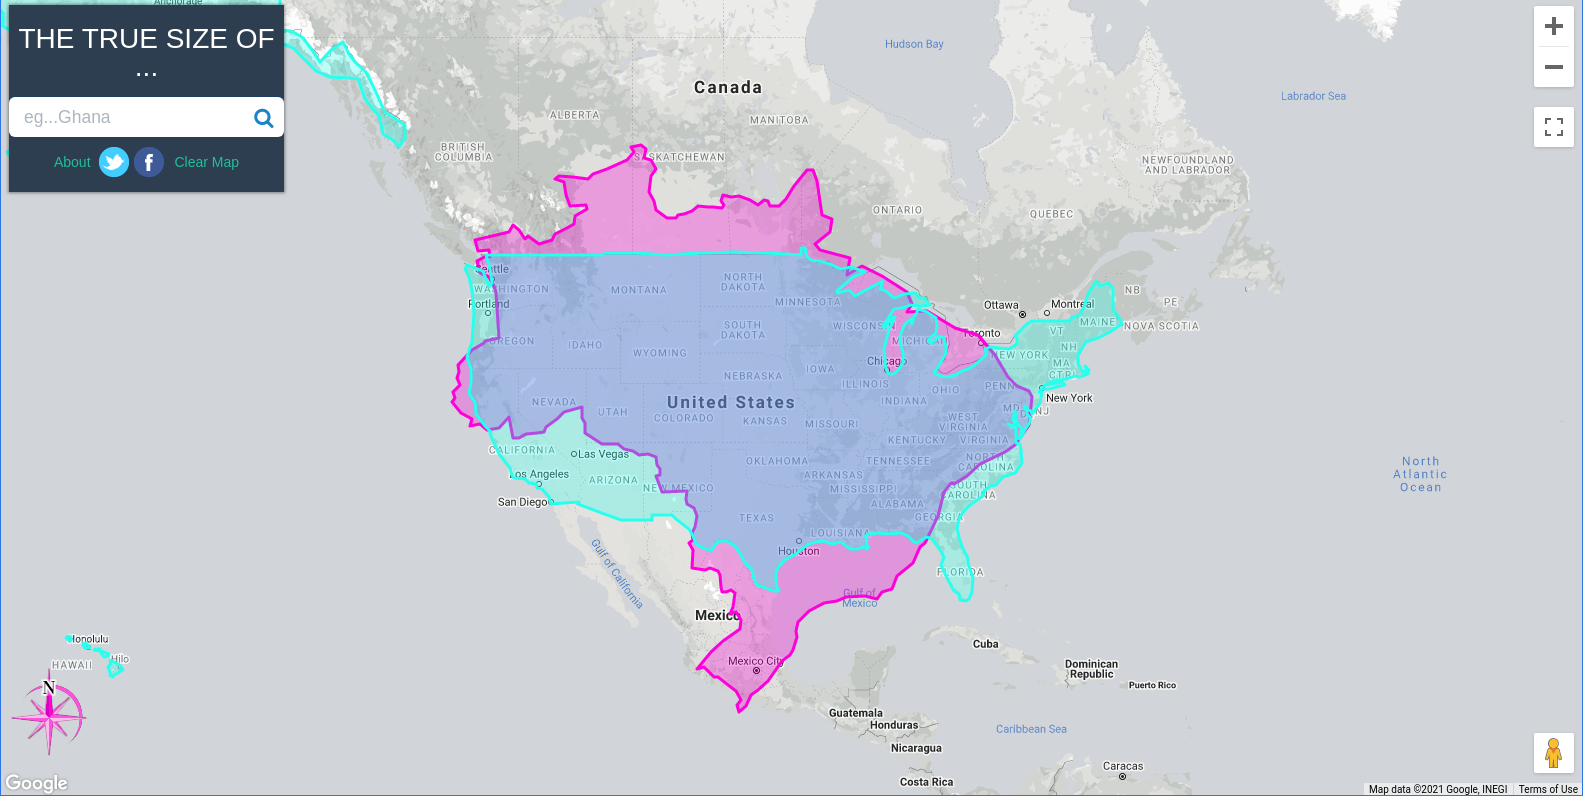
\includegraphics{media/modulo0/true-size-of.png}
\caption{True Size Of}
\end{figure}

\hypertarget{detalhando-os-conceitos}{%
\subsubsection{Detalhando os conceitos}\label{detalhando-os-conceitos}}

Então por que isso acontece? Como você aprenderá neste módulo, é difícil representar a forma tridimensional da Terra em uma folha de papel plana. Para fazer isso, os cartógrafos usam o que é chamado de \textbf{projeção cartográfica}, para projetar os pontos da superfície tridimensional da Terra em uma superfície plana. No entanto, ao fazer isso, eles introduzem alguma \textbf{distorção}. Essa distorção pode ser de forma, tamanho, direção e distâncias dos objetos representados no mapa. Todos os mapas têm pelo menos uma dessas distorções. Por causa dessa distorção, um mapa nunca pode mostrar toda a verdade sobre a Terra.

No mapa online que usamos, o mapa de fundo que não muda de tamanho (em cinza) é um exemplo de \textbf{dados raster}. Os dados raster são representações do mundo baseadas em pixels, semelhantes a como fotografias funcionam. Enquanto isso, a forma dos países que podemos mover são exemplos de \textbf{dados vetor, ou vetoriais}. Os dados vetoriais, ao contrário dos rasters, representam o mundo usando objetos discretos (no sentido matemático da palavra), como pontos, linhas e polígonos.

\hypertarget{conteuxfado-principal}{%
\subsection{Conteúdo principal}\label{conteuxfado-principal}}

\hypertarget{tuxedtulo-da-fase-1-mapas-e-coordenadas}{%
\subsubsection{Título da Fase 1: Mapas e Coordenadas}\label{tuxedtulo-da-fase-1-mapas-e-coordenadas}}

\hypertarget{conteuxfado-tutorial}{%
\paragraph{Conteúdo / Tutorial}\label{conteuxfado-tutorial}}

Quando as pessoas pensam na Terra atualmente, elas geralmente imaginam uma massa esférica azul, verde, branca e marrom flutuando no espaço. É por isso que tradicionalmente usamos globos para representar a Terra.

Figura 1. A Bola de Gude Azul ( https://commons.wikimedia.org/wiki/Earth\#/media/File:The\_Blue\_Marble.jpg)

Figura 2. Globo de l'Isle (1765) ( https://commons.wikimedia.org/wiki/Globe\#/media/File:3quarter\_globe.jpg)

No entanto, embora o globo seja capaz de capturar a maioria das características da Terra, ele possui duas desvantagens principais:

\begin{itemize}
\tightlist
\item
  Os globos são pesados e difíceis de transportar.
\item
  Os globos só podem ser usados em pequenas escalas (por exemplo, encontrar locais de países, as posições relativas de cidades, etc.). Eles são praticamente inúteis para atividades que exigem grandes escalas ou detalhes finos (por exemplo, navegação dentro de uma cidade).
\end{itemize}

É aqui que entram os mapas. Os mapas corrigem essas duas desvantagens dos globos, representando a Terra como uma superfície plana. Ao fazer isso, os mapas se tornam portáteis e adequados para uma infinidade de usos. Dito isso, os mapas também apresentam uma desvantagem própria. Através do processo de conversão de um objeto tridimensional (globo) em um bidimensional (mapa), distorções são geradas, de tal forma que é impossível para um mapa capturar perfeitamente as diferentes características da Terra (ou seja, formas, áreas e direções).

\hypertarget{projeuxe7uxf5es-cartogruxe1ficas}{%
\subparagraph{Projeções cartográficas}\label{projeuxe7uxf5es-cartogruxe1ficas}}

Uma projeção cartográfica é usada para achatar a superfície da Terra (ou de um globo qualquer) em um plano, a fim de criar um mapa. Este processo de transformação gera distorção.

\begin{figure}
\centering
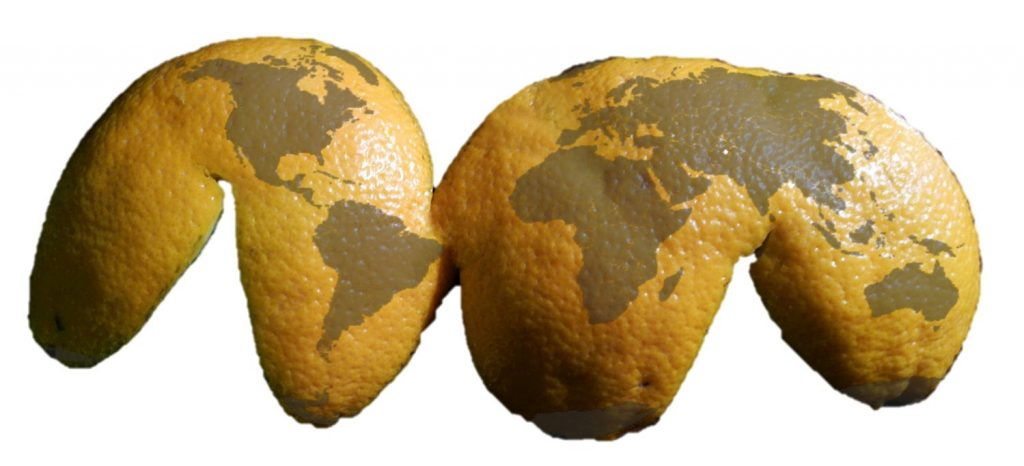
\includegraphics{media/modulo0/dalandan.png}
\caption{A terra como uma laranja}
\end{figure}

Pense na Terra como uma laranja. Se você descascá-la, poderá deixá-la plana, mas nunca poderá torná-la perfeitamente plana. Você sempre encontrará um dos seguintes problemas:

\begin{itemize}
\tightlist
\item
  \textbf{Alongamento} - o alongamento da casca (ou superfície) em uma ou mais direções
\item
  \textbf{Rasgos} - a divisão ou ruptura da casca (ou superfície)
\item
  \textbf{Compressão} - o encurtamento ou encolhimento da casca (ou superfície)
\end{itemize}

Por causa desses problemas, cada mapa contém distorção em uma ou mais das seguintes características:

\begin{itemize}
\tightlist
\item
  \textbf{Forma}
\item
  \textbf{Área}
\item
  \textbf{Distância}
\item
  \textbf{Direção}
\end{itemize}

As projeções cartográficas podem preservar (sem distorção) uma ou mais dessas características, mas nunca todas ao mesmo tempo. Outra opção é balancear e minimizar as distorções para todas as características ao mesmo tempo. Isso se deve à natureza das próprias características.

Características principais como \textbf{Forma} e \textbf{Área} são \textbf{mutuamente excludentes} e não podem ser preservadas simultaneamente. Enquanto isso, as características secundárias \textbf{Distância} e \textbf{Direção} \textbf{não têm como estar corretas em todos os lugares} do mapa.

Ao escolher qual projeção cartográfica usar, é importante que você considere o propósito do mapa. Por exemplo, se deseja realizar análises baseadas em área, é melhor usar uma projeção cartográfica que preserva a área.

Existem várias classificações de projeções cartográficas. A primeira é baseada nas \textbf{características que elas preservam}.

\begin{itemize}
\tightlist
\item
  Projeções de mapa \textbf{conforme} ou \textbf{ortomórficas} são aquelas que preservam a forma ou a conformidade angular. Estes são comumente usados para fins de navegação ou meteorológicos. As formas são preservadas, mas as áreas são distorcidas. Quanto maior a área, maior a distorção.
\item
  Projeções de mapa de \textbf{equivalente} ou \textbf{de igual área} são aquelas que preservam a proporção ou áreas relativas dos objetos no mapa. Nesse tipo de projeção cartográfica, quanto maior a área mapeada, mais precisa ela será.
\item
  As projeções cartográficas \textbf{equidistantes} preservam a distância das linhas que originam em um ou dois pontos no mapa ou têm escala adequada ao longo de uma ou mais linhas.
\item
  As projeções cartográficas \textbf{azimutais} preservam a direção a partir de um ou dois pontos no mapa. São úteis para mapear rotas de aeronaves e embarcações marítimas entre portos.
\end{itemize}

Uma única projeção cartográfica pode preservar mais de uma característica (por exemplo, uma projeção azimutal equidistante que preserva a direção e as distâncias a partir de um ou dois pontos no mapa), mas nem todas delas, como mostrado na tabela abaixo.

Conforme

Equivalente

Equidistante

Azimutal

Conforme

\begin{itemize}
\item
  Não

  Não

  Sim

  Equivalente

  Não

  \begin{itemize}
  \item
    Não

    Sim

    Equidistante

    Não

    Não

    \begin{itemize}
    \item
      Sim

      Azimutal

      Sim

      Sim

      Sim

      \begin{itemize}
      \tightlist
      \item
      \end{itemize}
    \end{itemize}
  \end{itemize}
\end{itemize}

Tabela: Ambas características podem ser preservadas por um mapa ao mesmo tempo?

Existe outra classificação de projeções cartográficas que não preserva nenhuma das características do mapa, mas tenta minimizar todas as distorções no mapa. Estes são chamados de projeções \textbf{Erro Mínimo (Minimum Error, ou Compromise)} (mapas que não preservam a forma nem a área são chamados de \textbf{Afiláticos}).

Uma maneira de visualizar a distorção é usando o que é chamado de \textbf{indicador de Tissot}. Este indicador caracteriza as distorções locais usando círculos e mostrando como esses círculos são transformados ao longo do mapa.

\begin{figure}
\centering
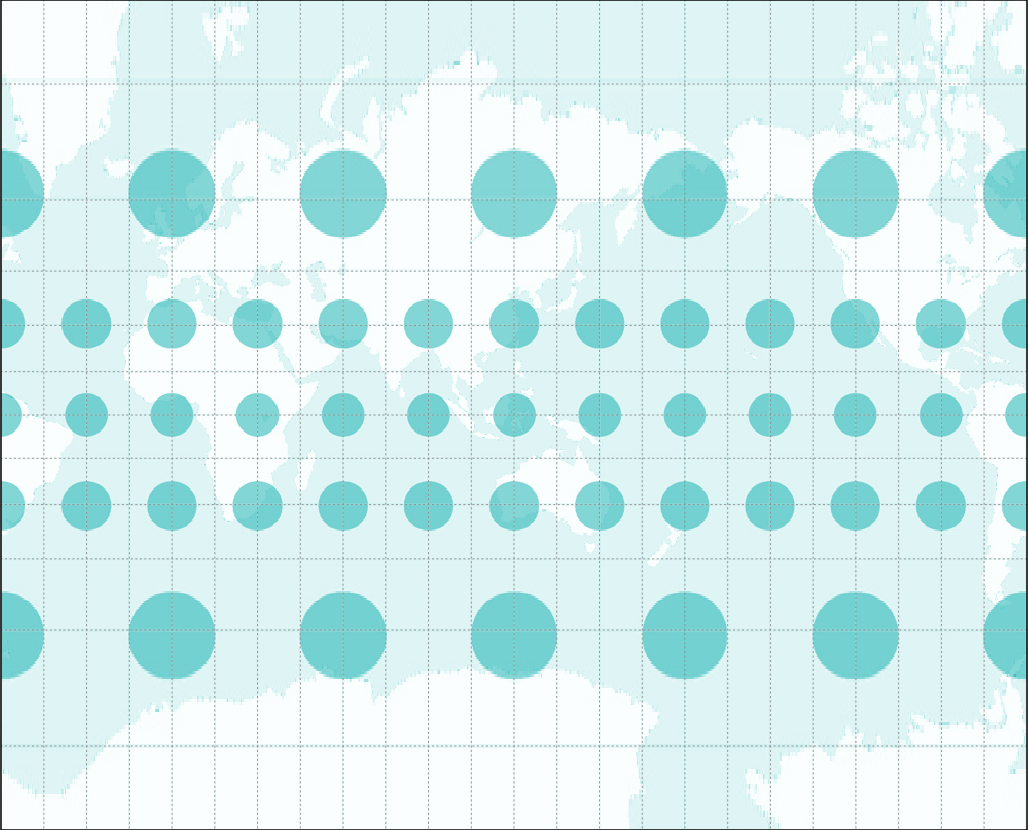
\includegraphics{media/modulo0/conformal.png}
\caption{Projeção conforme}
\end{figure}

Figura 3. Projeção conforme com seu índice de Tissot. Os círculos permanecem como círculos por todo o mapa, mas suas áreas aumentam a medida que os círculos se movem do equador em direção aos pólos.

\begin{figure}
\centering
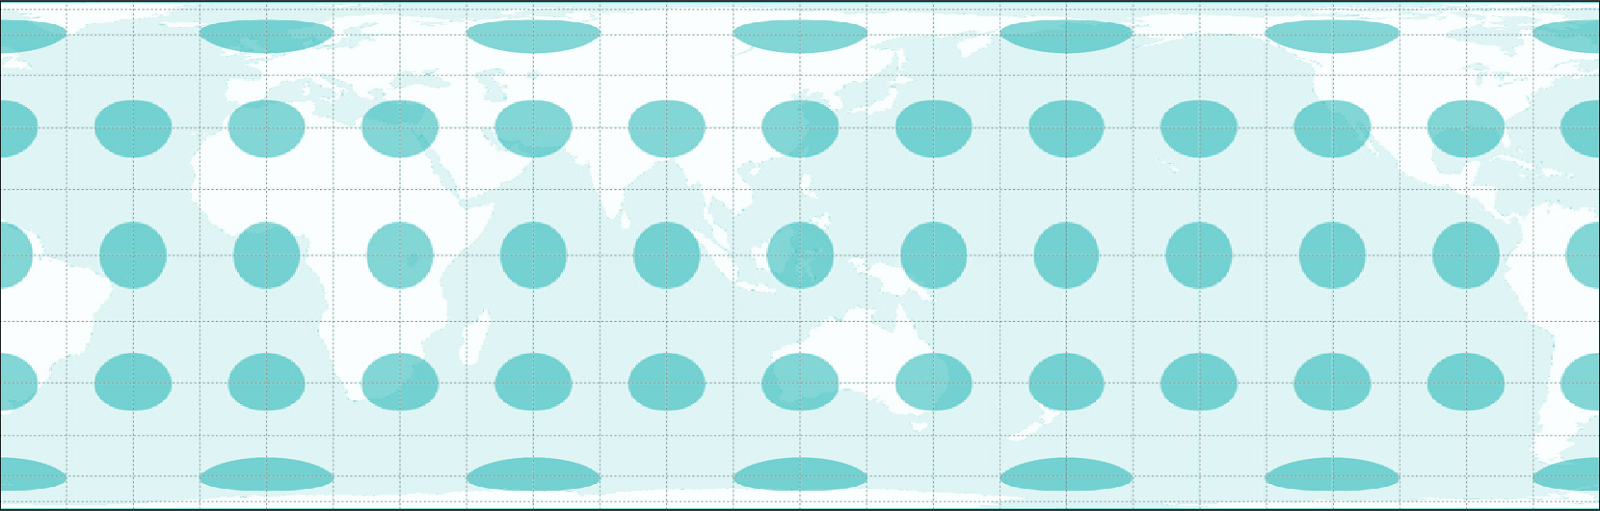
\includegraphics{media/modulo0/authalic.png}
\caption{Projeção equivalente}
\end{figure}

Figura 4. Projeção equivalente com seu índice de Tissot. Os círculos tornam-se elipses, mas suas áreas permanecem as mesmas.

\begin{figure}
\centering
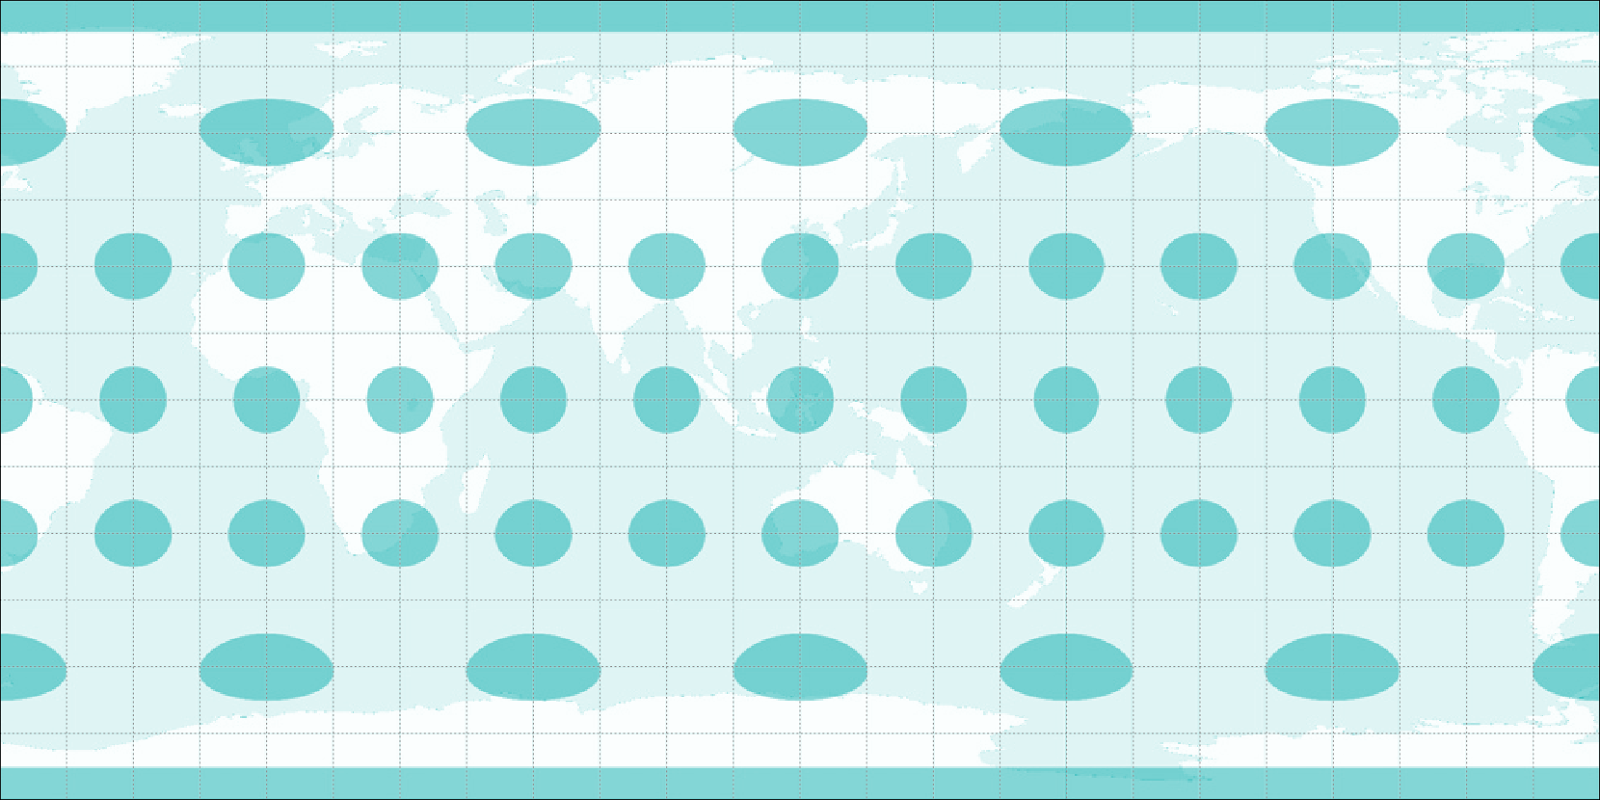
\includegraphics{media/modulo0/equidistant.png}
\caption{Projeção equidistante}
\end{figure}

Figura 5. Projeção equidistante com seu índice de Tissot. Observe que as alturas dos círculos são iguais, o que significa que a escala / distâncias ao longo dos meridianos são preservadas.

\begin{figure}
\centering

\includegraphics{media/modulo0/az-equidistant.png}
\caption{Projeção azimutal equidistante}
\end{figure}

Figura 6. Projeção azimutal equidistante com seu índice de Tissot. Observe que os círculos estão todos apontando para o centro do mapa e as alturas dos círculos são todas iguais.

Outra maneira de classificar as projeções do mapa é pela \textbf{superfície desenvolvível (``developable surface'')} usada para criar o mapa. Uma superfície é desenvolvível se ela puder ser planificada sem introduzir distorções. As superfícies mais comumente usadas são: Cilindros (Figura 7), Cones (Figura 8) e Planos (Figura 9).

\begin{figure}
\centering
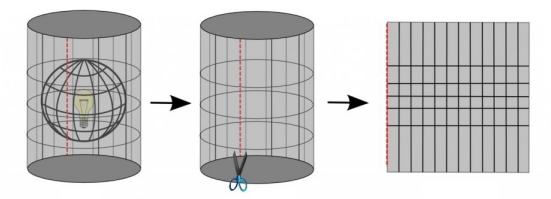
\includegraphics{media/modulo0/cylinder.png}
\caption{Cilindro como uma superfície desenvolvível}
\end{figure}

Figura 7. As projeções cilíndricas têm meridianos (longitude) e paralelos (latitude) encontrando-se em ângulos retos com as distâncias entre os meridianos sendo iguais.

\begin{figure}
\centering
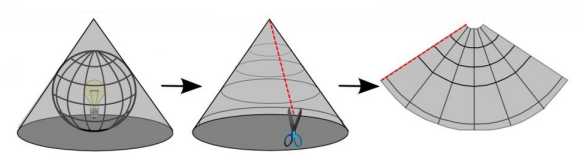
\includegraphics{media/modulo0/cone.png}
\caption{Cone como superfície desenvolvível}
\end{figure}

Figura 8. As projeções cônicas têm meridianos retos indo para um ponto nos pólos. Os paralelos são arcos.

\begin{figure}
\centering
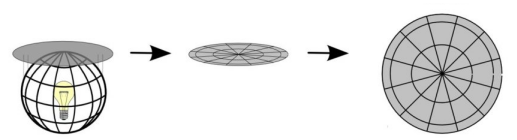
\includegraphics{media/modulo0/plane.png}
\caption{Plano como superfície desenvolvível}
\end{figure}

Figura 9. As projeções planas (comumente usadas em projeções azimutais) têm meridianos retos semelhantes às projeções cônicas, mas seus paralelos são círculos em vez de arcos.

Existem inúmeras outras superfícies desenvolvíveis que podem ser usadas para transformar um globo em um mapa. Eles podem ser uma variação das superfícies comuns, como no caso de projeções pseudo-cilíndricas e pseudo-cônicas ou podem ser superfícies únicas e diferentes, como no mapa Dymaxion, que usa um icosaedro (poliedro com 20 faces), ou a Projeção de Cahill-Keyes que usa um octaedro (poliedro com 8 faces).

A projeção de um mapa também pode ser classificada de acordo com seu \textbf{aspecto} (Figura 10) ou o modo como a superfície desenvolvível está posicionada no globo: Normal, Transversal ou Oblíqua.

\begin{figure}
\centering
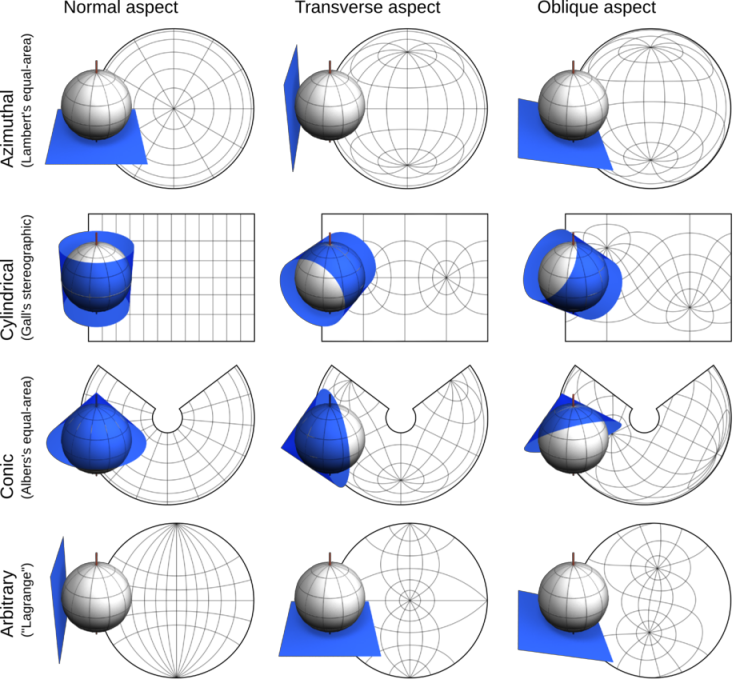
\includegraphics{media/modulo0/aspects.png}
\caption{Aspectos de uma projeção cartográfica}
\end{figure}

Figura 10. Aspectos de uma projeção cartográfica

\hypertarget{sistemas-de-referuxeancia-de-coordenadas}{%
\subparagraph{Sistemas de referência de coordenadas}\label{sistemas-de-referuxeancia-de-coordenadas}}

Um \textbf{Sistema de Referência de Coordenadas (SRC, ou CRS na sigla em inglês)} é usado para especificar a localização de um objeto na superfície da Terra por meio do uso de coordenadas. SRCs podem ser classificados em dois:

\begin{itemize}
\tightlist
\item
  \textbf{Sistemas de referência de coordenadas geográficas} usam graus de latitude e longitude como coordenadas para se referir à posição.
\item
  \textbf{Sistemas de referência de coordenadas projetadas} usam unidades lineares (por exemplo, metros, pés, quilômetros) de leste e norte como coordenadas.
\end{itemize}

O conhecimento dos sistemas de referência de coordenadas é importante porque mesmo que dois mapas (ou camadas) mostrem o mesmo local, as coordenadas das localizações nesses mapas serão diferentes se os SRC que eles usam forem diferentes.

\textbf{Veja este exemplo:} Mapa A e Mapa B mostram a mesma área e extensão. Eles são basicamente o mesmo mapa. A única diferença é o sistema de referência de coordenadas que eles usam. O Mapa A usa SRC X e o Mapa B usa SRC Y. Digamos que obtivemos a coordenada do Ponto 1, que é (10, 10), do Mapa A. Se olharmos para a coordenada (10,10) no Mapa B, é possível que o Ponto 1 não esteja lá, pois o Mapa B usa um SRC diferente. Ou, se você sobrepor os mapas um ao outro usando uma referência comum, os objetos dos dois mapas não coincidirão. Este conhecimento de sistemas de referência de coordenadas é importante para qualquer tipo de GIS.

As versões do QGIS anteriores à versão 3 tinham a opção de ativar o que é chamado de ``OTF'' ou ``Transformação On-The-Fly (em `tempo real')''. Isso permitia que camadas com diferentes SRC fossem projetadas na tela do mapa como se estivessem no mesmo SRC. Com o QGIS 3 em diante, esta opção é ativada automaticamente como comportamento padrão do QGIS. QGIS também executa esta ação automaticamente para tarefas de processamento. Isso é muito importante porque se as camadas não estiverem no mesmo SRC, os resultados das consultas espaciais e do processamento como junções espaciais, clipes, etc. podem ser comprometidos.

Você pode notar que alguns Sistemas de Referência de Coordenadas são referidos por seu Código EPSG. Este código se refere ao código do SRC no conjunto de dados de parâmetros geodésicos EPSG, que é um registro de dados geodésicos, sistemas de referência espacial, elipsóides terrestres, transformações de coordenadas e unidades de medida relacionadas. A maioria dos GIS, incluindo QGIS, referem-se ao código EPSG para identificar sistemas de referência de coordenadas, projeções e realizar transformações entre esses sistemas.

Alguns códigos EPSG comuns incluem:

\begin{itemize}
\tightlist
\item
  \textbf{EPSG: 4326} - WGS 84, sistema de coordenadas de latitude / longitude baseado no Sistema de Posicionamento Global (GPS) entre outros.
\item
  \textbf{EPSG: 3857} - Projeção Web Mercator usada para exibição por muitas ferramentas de mapeamento baseadas na web, como OpenStreetMap e Google Maps
\item
  \textbf{EPSG: 31973 a EPSG: 31974 e EPSG: 31978 a EPSG: 31985} - Universal Transverse Mercator (UTM) Zonas 19N a 20N, e 18S a 25S. Zonas UTM usadas no Brasil
\item
  \textbf{EPSG: 4674} - Sistema de Referência SIRGAS 2000, utilizado nas Américas a partir do ano 2000
\end{itemize}

\hypertarget{quiz}{%
\paragraph{Quiz}\label{quiz}}

\begin{enumerate}
\def\labelenumi{\arabic{enumi}.}
\tightlist
\item
  Que tipo de projeção é melhor para os seguintes casos?

  \begin{enumerate}
  \def\labelenumii{\arabic{enumii}.}
  \tightlist
  \item
    um mapa de uso geral que precisa ter uma aparência agradável
  \item
    um mapa mostrando uma análise de área por unidade entre diferentes locais
  \item
    um mapa que mostra uma comparação de uma zona de 10 km de raio de diferentes locais
  \end{enumerate}
\item
  Que tipo de sistema de referência de coordenadas (geográfico ou projetado) é melhor utilizado para os seguintes casos?

  \begin{enumerate}
  \def\labelenumii{\arabic{enumii}.}
  \setcounter{enumii}{3}
  \tightlist
  \item
    mostrar a localização de pontos usando GPS
  \item
    calcular a distância entre dois pontos
  \end{enumerate}
\item
  Verdadeiro ou falso - É possível preservar as seguintes características do mapa juntas em um único mapa:

  \begin{enumerate}
  \def\labelenumii{\arabic{enumii}.}
  \setcounter{enumii}{5}
  \tightlist
  \item
    Área e forma
  \item
    Distância e direção
  \end{enumerate}
\end{enumerate}

\hypertarget{tuxedtulo-da-fase-2-tipos-de-dados-espaciais}{%
\subsubsection{Título da fase 2: Tipos de dados espaciais}\label{tuxedtulo-da-fase-2-tipos-de-dados-espaciais}}

\hypertarget{conteuxfado-tutorial-1}{%
\paragraph{Conteúdo / Tutorial}\label{conteuxfado-tutorial-1}}

Em sua essência, um Sistema de Informação Geográfica (SIG) deve ser capaz de modelar objetos, informações e fenômenos do mundo real, como limites de lotes, rios, estradas, temperatura, etc. Ele faz isso por meio de modelos de dados espaciais.

Os modelos de dados espaciais são compostos de dois componentes principais que, quando combinados, modelam a realidade. Esses componentes são:

\begin{itemize}
\tightlist
\item
  \textbf{Feições espaciais (ou geometria)}
\item
  \textbf{Atributos}
\end{itemize}

\begin{figure}
\centering
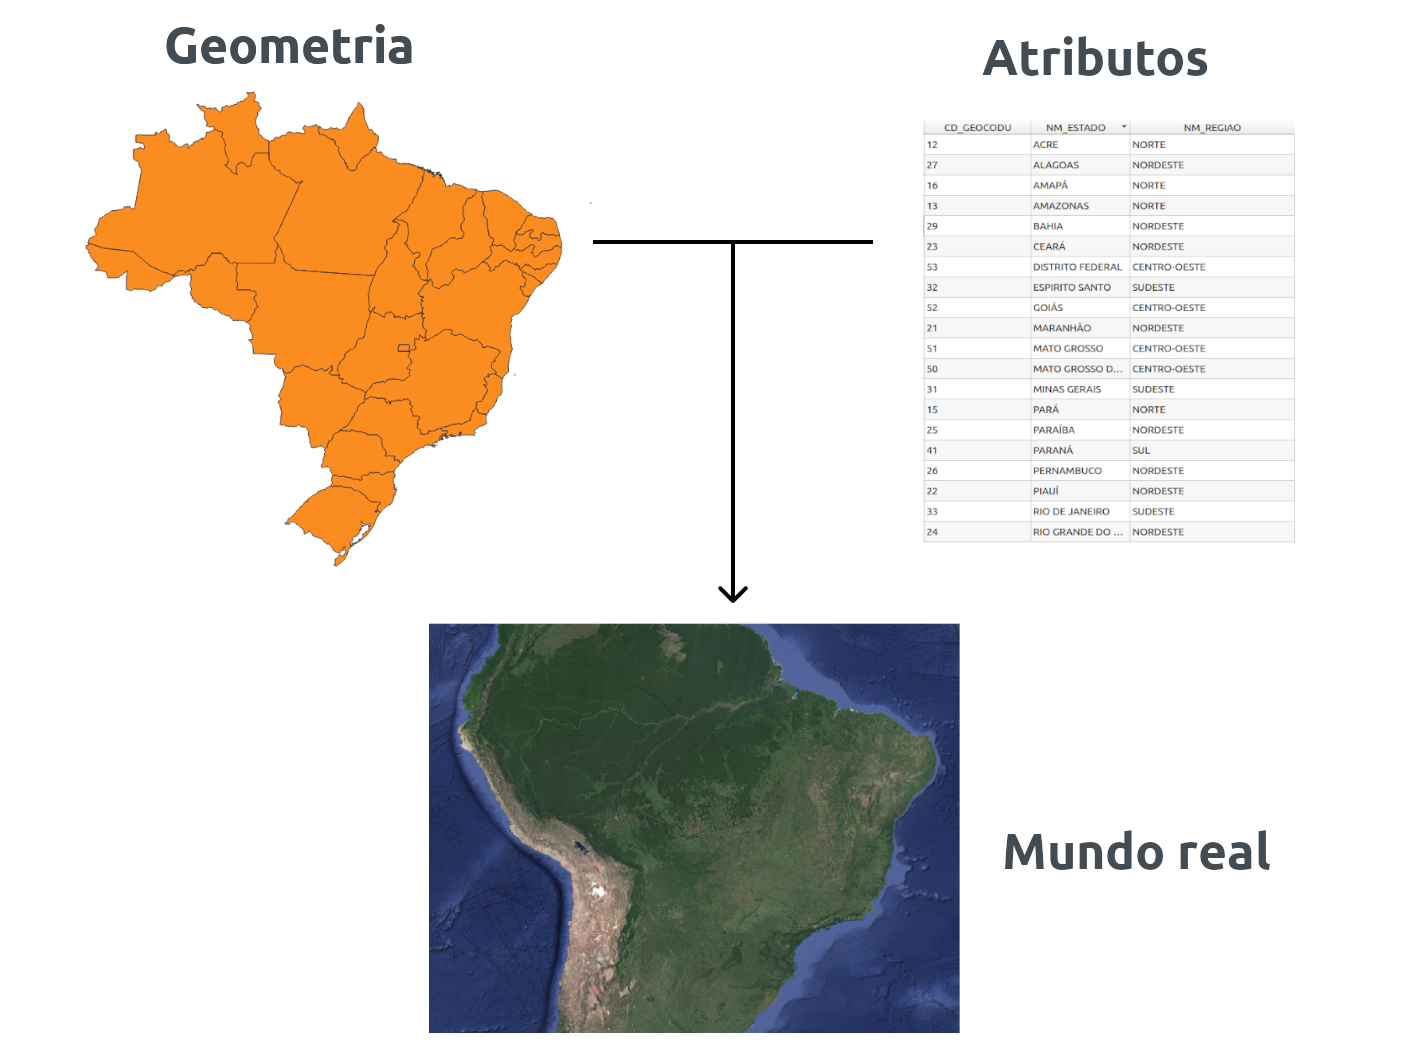
\includegraphics{media/modulo0/spatial-model.png}
\caption{Modelo de dados espaciais}
\end{figure}

Existem dois modelos principais de dados espaciais: \textbf{raster} e \textbf{vetorial}. Embora qualquer objeto do mundo real possa ser representado por qualquer um dos dois modelos de dados, um deles é geralmente melhor para representar certos objetos do mundo real do que o outro.

\hypertarget{dados-raster}{%
\subparagraph{Dados raster}\label{dados-raster}}

Os dados raster são mais utilizados para representar fenômenos contínuos, como elevação ou temperatura.

Um raster é uma representação de objetos do mundo real composta de linhas e colunas de células ou pixels, no qual cada célula ou pixel representa uma área geográfica (pense em uma fotografia ou imagem). O valor da célula representa o valor de um atributo na referida área geográfica. O tamanho da área depende da resolução espacial do raster.

Rasters são bastante úteis para modelagem de adequação de locais (suitability modelling), pois você pode combinar rasters por meio de operações matemáticas (álgebra de raster).

\begin{figure}
\centering
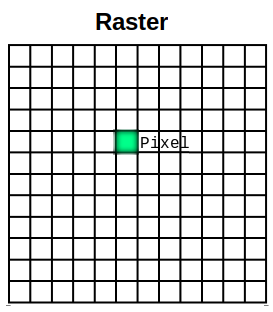
\includegraphics{media/modulo0/raster.png}
\caption{Modelo de dados raster}
\end{figure}

Figura 12. Um raster consiste em pixels de tamanhos iguais em linhas e colunas.

Um pixel raster pode conter apenas um valor de cada vez. Assim, um raster pode modelar apenas um objeto ou fenômeno por vez.

\hypertarget{dados-vetoriais}{%
\subparagraph{Dados vetoriais}\label{dados-vetoriais}}

Os dados vetoriais são mais utilizados para representar objetos discretos.

Os dados vetoriais possuem três formas: ponto, linha e polígono. São mais preciso que rasters porque pontos, linhas e polígonos são modelados usando coordenadas bem definidas, tornando-os melhores na representação de objetos discretos do que rasters.

Os vetores são comumente usados quando necessitamos precisão com comprimentos, áreas e distâncias. Eles também são úteis ao realizar análises de rede (por exemplo, encontrar o caminho mais curto um ponto a outro em uma rede de vias).

\begin{figure}
\centering
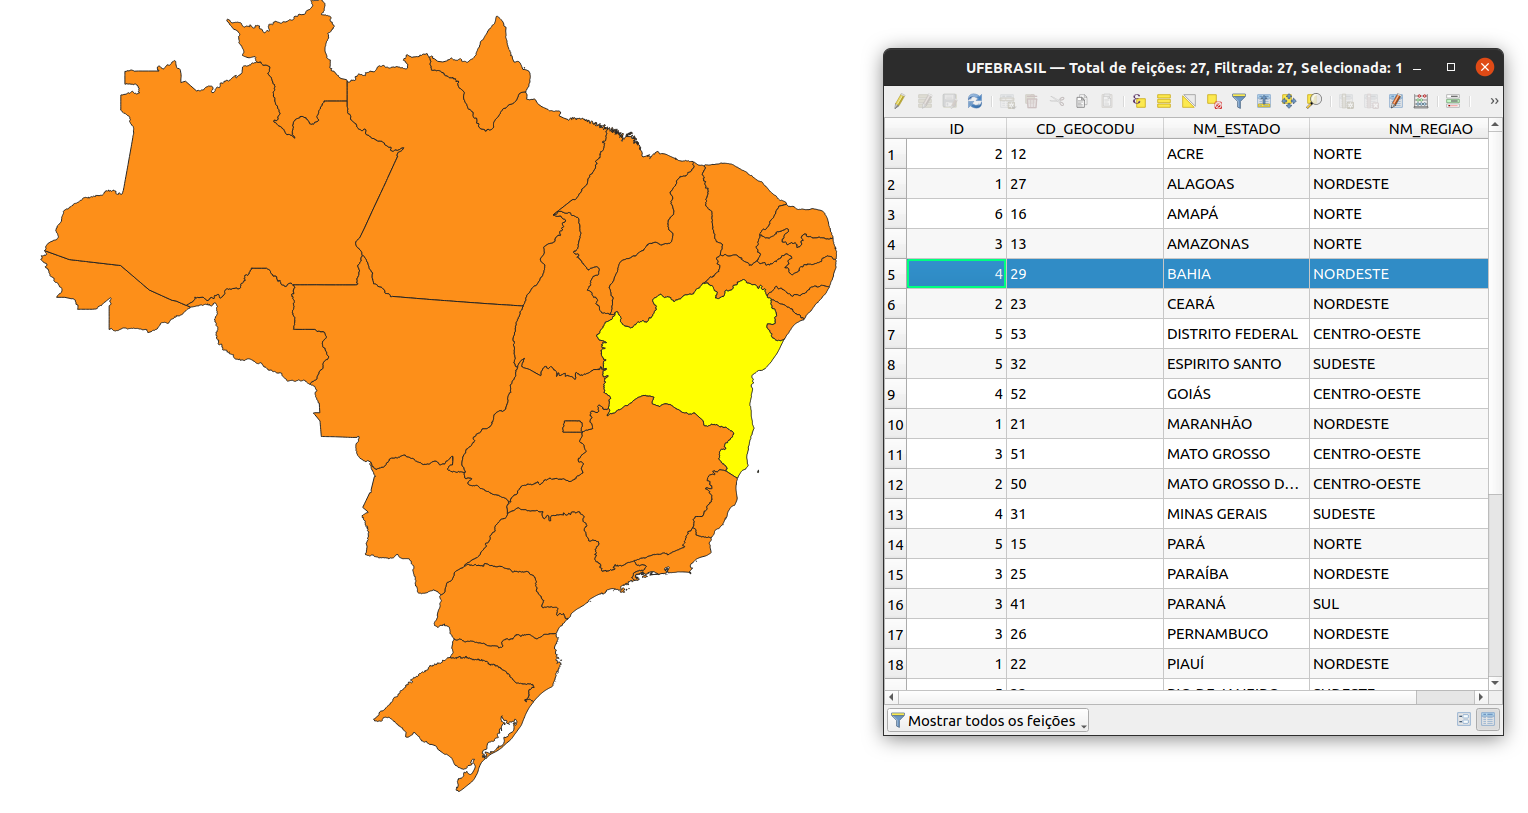
\includegraphics{media/modulo0/vector.png}
\caption{Modelo de dados vetoriais}
\end{figure}

Figura 13. Um vetor consiste em feições com seus atributos correspondentes.

Comparado aos pixels raster, uma feição vetorial pode conter mais de um valor por vez. Esses valores são armazenados como colunas na tabela de atributos. Cada feição é armazenada como uma linha.

\hypertarget{quiz-1}{%
\paragraph{Quiz}\label{quiz-1}}

\begin{enumerate}
\def\labelenumi{\arabic{enumi}.}
\tightlist
\item
  Qual tipo de dado pode representar melhor os seguintes objetos / fenômenos:

  \begin{enumerate}
  \def\labelenumii{\arabic{enumii}.}
  \tightlist
  \item
    estradas
  \item
    casas
  \item
    densidade populacional
  \item
    perigo de inundação
  \end{enumerate}
\end{enumerate}

\hypertarget{tuxedtulo-da-fase-3-sistema-de-informauxe7uxe3o-geogruxe1fica-sig}{%
\subsubsection{Título da Fase 3: Sistema de Informação Geográfica (SIG)}\label{tuxedtulo-da-fase-3-sistema-de-informauxe7uxe3o-geogruxe1fica-sig}}

\hypertarget{conteuxfado-tutorial-2}{%
\paragraph{Conteúdo / Tutorial}\label{conteuxfado-tutorial-2}}

As informações geográficas e de localização tornaram-se onipresentes no século 21 em todos os níveis de granularidade. Temos satélites, aeronaves e até drones comerciais que são capazes de capturar grandes quantidades de dados brutos em grandes áreas por longos períodos de tempo. Existem também sensores que coletam e reúnem informações de localização, como o GPS e outros aplicativos em nossos telefones e dispositivos.

Com todos esses dados à nossa disposição, é fundamental saber gerenciá-los, analisá-los e apresentá-los. É aqui que entram os Sistemas de Informação Geográfica, ou mais comumente conhecidos como SIG, ou GIS.

SIG é uma ferramenta / framework / sistema que nos permite trabalhar com informação geográfica (ou espacial) e sua correspondente informação de atributo (não espacial). Em particular, um GIS deve ser capaz de:

\begin{itemize}
\tightlist
\item
  \textbf{Coletar}, \textbf{armazenar}, \textbf{editar}, \textbf{manipular}, ou em termos mais gerais, \textbf{gerenciar} dados espaciais.
\item
  \textbf{Analizar} os dados usando seu componente espacial (onde os dados estão) ou atributo (o valor dos dados).
\item
  \textbf{Apresentar} os dados e análises como informações significativas por meio de mapas, gráficos, plotagens e outras visualizações.
\end{itemize}

\emph{SIG não é apenas mapeamento}. Embora a elaboração de mapas seja um dos aspectos mais importantes e comumente conhecidos do SIG, ela ainda é apenas uma parte de seus muitos recursos. Podemos ver a estrutura SIG moderna como sendo composta por:

\begin{itemize}
\tightlist
\item
  \textbf{Dados} - referem-se às informações utilizadas pelo SIG que podem ou não conter informações de localização (por exemplo, nomes de lojas, localizações de lojas).
\item
  \textbf{Tecnologia} - inclui os componentes de hardware e software de um SIG - as máquinas, instrumentos e computadores com os aplicativos de software usados para fazer o trabalho geoespacial.
\item
  \textbf{Métodos e análises} - referem-se à ciência e matemática em SIG, que permitem realizar consultas e cálculos espaciais e não espaciais (de atributos).
\item
  \textbf{Visualização} - embora semelhante aos métodos e análises, a visualização pode ser considerada como um componente separado, pois se refere especificamente aos meios pelos quais um SIG representa os dados graficamente. Isso inclui não apenas mapas, embora seja o caso mais comum, mas também tabelas, gráficos, etc.
\item
  \textbf{Pessoas} - são as pessoas e / ou grupos de pessoas que estão envolvidas no uso, desenvolvimento, ensino e manutenção de SIG.
\end{itemize}

Todas as partes da estrutura SIG moderna - dos dados às pessoas - são essenciais para garantir seu sucesso.

\hypertarget{perguntas-do-questionuxe1rio}{%
\paragraph{Perguntas do questionário}\label{perguntas-do-questionuxe1rio}}

\begin{enumerate}
\def\labelenumi{\arabic{enumi}.}
\tightlist
\item
  Verdadeiro ou falso:

  \begin{enumerate}
  \def\labelenumii{\arabic{enumii}.}
  \tightlist
  \item
    Um SIG só pode ser usado com dados geoespaciais.
  \item
    Um mapa é sempre o resultado ao se usar um SIG.
  \item
    Aprender SIG é difícil e caro.
  \end{enumerate}
\end{enumerate}

\hypertarget{tuxedtulo-da-fase-4-adicional-software-livre-e-de-cuxf3digo-aberto-para-uso-geoespacial-foss4g}{%
\subsubsection{Título da Fase 4 (adicional): Software Livre e de Código Aberto para uso Geoespacial (FOSS4G)}\label{tuxedtulo-da-fase-4-adicional-software-livre-e-de-cuxf3digo-aberto-para-uso-geoespacial-foss4g}}

\hypertarget{conteuxfado-tutorial-3}{%
\paragraph{Conteúdo / Tutorial}\label{conteuxfado-tutorial-3}}

QGIS é apenas um exemplo de software livre e de código aberto para uso geoespacial (FOSS4G). Outros exemplos de FOSS4G são GRASS, PostGIS, GeoServer, GeoNode, etc. Esses aplicativos FOSS4G são ótimas ferramentas para trabalhar não só porque são confiáveis, mas também porque, sendo gratuitos e de código aberto, têm uma barreira de entrada menor e são altamente personalizáveis para qualquer necessidade. Você pode encontrar uma variedade de softwares geoespaciais gratuitos e de código aberto para cada necessidade e para cada parte do ``stack'' geoespacial.

\begin{figure}
\centering
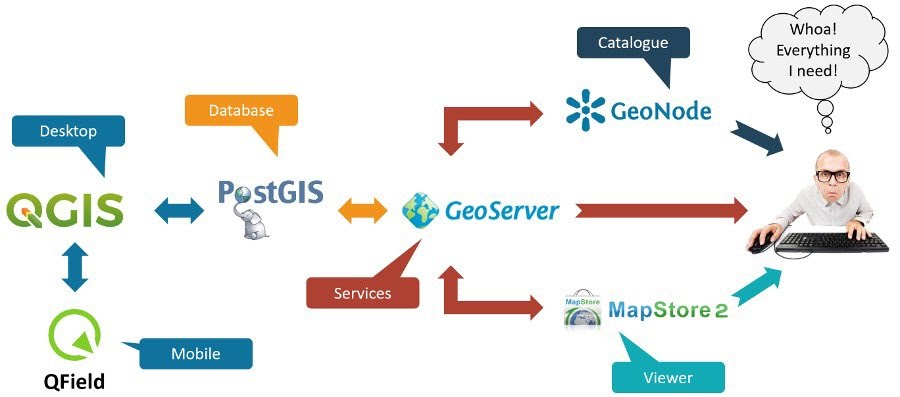
\includegraphics{media/modulo0/foss4g-stack.jpeg}
\caption{Stack de aplicativos de software livre e de código aberto para geoespaciais (FOSS4G)}
\end{figure}

Figura 14. Uma amostra de stack geoespacial de código aberto (ou FOSS4G) (de Simon Nitz (\url{https://twitter.com/si_nitz?lang=en}))

\hypertarget{software-gruxe1tis}{%
\subparagraph{Software grátis}\label{software-gruxe1tis}}

\textbf{Livre como em liberdade e não apenas grátis.}

Software livre é o software que adere às Quatro Liberdades Essenciais do Software Livre, que são:

\begin{enumerate}
\def\labelenumi{\arabic{enumi}.}
\tightlist
\item
  A liberdade de executar o programa como desejar, para qualquer propósito (liberdade 0).
\item
  A liberdade de estudar como o programa funciona e alterá-lo para que ele faça o que você deseja (liberdade 1). O acesso ao código-fonte é uma pré-condição para isso.
\item
  A liberdade de redistribuir cópias para que você possa ajudar outras pessoas (liberdade 2).
\item
  A liberdade de distribuir cópias de suas versões modificadas para outros (liberdade 3). Ao fazer isso, você pode dar a toda a comunidade a chance de se beneficiar com suas mudanças. O acesso ao código-fonte é uma pré-condição para isso.
\end{enumerate}

\hypertarget{cuxf3digo-aberto}{%
\subparagraph{Código aberto}\label{cuxf3digo-aberto}}

Softwares de código aberto são aqueles que possuem licenças que permitem uso sem precisar pagar royalties e que permitem a reutilização do software, juntamente com acesso livre ao código-fonte. Por convenção, essas licenças de código aberto são aquelas que estão em conformidade com a definição de código aberto prevista pela Open Source Initiative. O código-fonte aberto não só garante acesso gratuito ao software e código-fonte, mas também a capacidade de redistribuir o software sem custos adicionais.

Por causa da natureza aberta do software de código aberto, ele também é um ótimo modelo de desenvolvimento de software, no qual todos são livres para atualizar, melhorar, modificar e compartilhar suas modificações com a comunidade.

\hypertarget{osgeo}{%
\subparagraph{OSGeo}\label{osgeo}}

Existem muitos softwares geoespaciais de código aberto e, às vezes, a parte mais difícil é saber onde e como começar a trabalhar com esses softwares. Felizmente, a Open Source Geospatial Foundation (OSGeo) (\url{https://www.osgeo.org/}) existe para ajudar a promover a adoção global de tecnologia geoespacial aberta e apoiar o desenvolvimento dessas tecnologias.

\hypertarget{perguntas-do-questionuxe1rio-1}{%
\paragraph{Perguntas do questionário}\label{perguntas-do-questionuxe1rio-1}}

N/D

\hypertarget{se-vocuxea-quiser-ir-mais-longe}{%
\subsubsection{Se você quiser ir mais longe}\label{se-vocuxea-quiser-ir-mais-longe}}

Se você quiser testar usar aplicativos FOSS4G facilmente, experimente o OSGeoLive (\url{https://live.osgeo.org/en/index.html}) que é uma distribuição Linux (sistema operacional) que vem pré-instalado com QGIS, GRASS e outros aplicativos FOSS4G.

\hypertarget{para-praticar-suas-novas-habilidades-tente}{%
\subsubsection{Para praticar suas novas habilidades, tente\ldots{}}\label{para-praticar-suas-novas-habilidades-tente}}

N/D

\hypertarget{dicas}{%
\subsubsection{Dicas}\label{dicas}}

N/D

\hypertarget{introduuxe7uxe3o-ao-qgis}{%
\chapter{Introdução ao QGIS}\label{introduuxe7uxe3o-ao-qgis}}

\textbf{Autor}: Ben Hur

\hypertarget{introduuxe7uxe3o-pedaguxf3gica-1}{%
\section{Introdução Pedagógica}\label{introduuxe7uxe3o-pedaguxf3gica-1}}

Este módulo serve como uma introdução ao QGIS. No final deste módulo, os alunos devem estar familiarizados com:

\begin{itemize}
\tightlist
\item
  O que é o QGIS
\item
  Interface do QGIS
\item
  Configurações do QGIS
\item
  Complementos do QGIS
\end{itemize}

Eles também devem aprender:

\begin{itemize}
\tightlist
\item
  Como instalar e abrir o QGIS
\item
  As diferentes partes e recursos da interface do QGIS
\item
  Como editar o layout e o tema da interface
\item
  As diferentes configurações do QGIS, como alterá-las e como elas afetam o QGIS
\item
  O que são perfis de usuário e como usá-los
\item
  O que são complementos e como instalá-los
\end{itemize}

O módulo também irá discutir algumas nuances do QGIS e o que o torna único ou diferente de outros softwares GIS, como formatos de arquivo QGIS.

\hypertarget{ferramentas-e-recursos-necessuxe1rios-1}{%
\section{Ferramentas e recursos necessários}\label{ferramentas-e-recursos-necessuxe1rios-1}}

As ferramentas e recursos necessários para este módulo são:

\begin{itemize}
\tightlist
\item
  Computador
\item
  Conexão de internet
\item
  QGIS 3.16 instalado no computador (\url{https://qgis.org/en/site/forusers/download.html})
\end{itemize}

\hypertarget{pruxe9-requisitos-1}{%
\section{Pré-requisitos}\label{pruxe9-requisitos-1}}

\begin{itemize}
\tightlist
\item
  Conhecimento básico de informática
\end{itemize}

\hypertarget{recursos-adicionais-1}{%
\section{Recursos adicionais}\label{recursos-adicionais-1}}

\begin{itemize}
\tightlist
\item
  Manual do usuário QGIS - \url{https://docs.qgis.org/3.16/en/docs/user_manual/}
\item
  Manual de treinamento QGIS - \url{https://docs.qgis.org/3.16/en/docs/training_manual/index.html}
\end{itemize}

\hypertarget{introduuxe7uxe3o-temuxe1tica-1}{%
\section{Introdução temática}\label{introduuxe7uxe3o-temuxe1tica-1}}

O mapa abaixo (\url{https://flic.kr/p/2jFfGJP}), de Andrés Felipe Lancheros Sánchez, mostra partes da cidade de Bogotá na Colômbia feitas no estilo da pintura ``Noite estrelada'' de Vincent van Gogh.

\begin{figure}
\centering
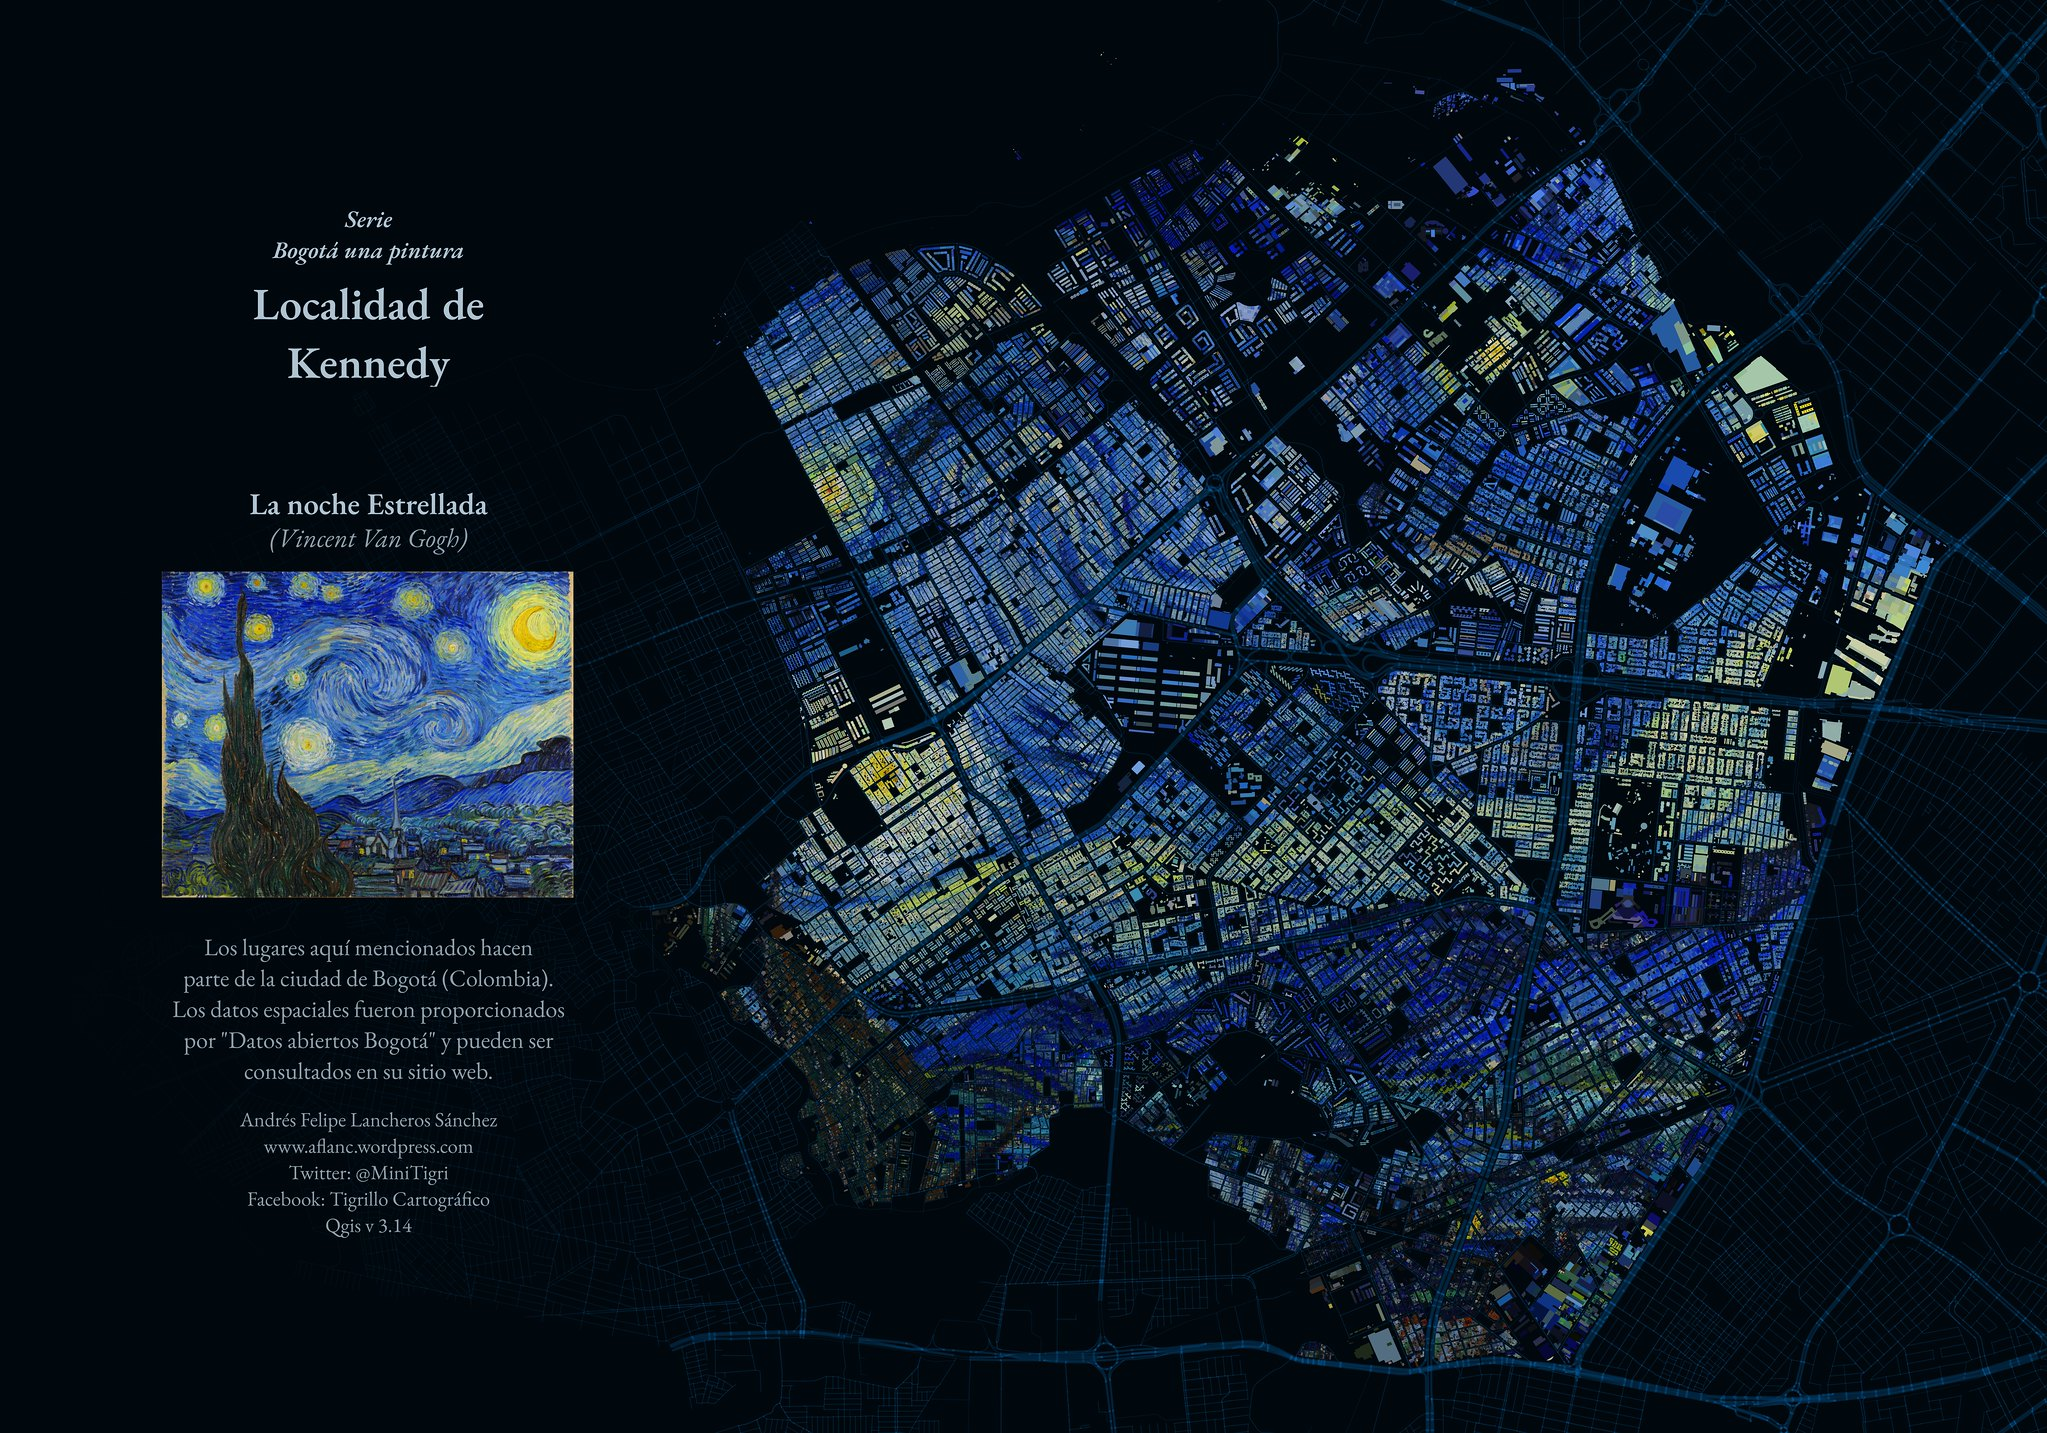
\includegraphics{media/modulo1/sample-1.jpg}
\caption{Mapa de Bogotá, Colômbia no estilo Noite Estrelada}
\end{figure}

Este próximo mapa (\url{https://flic.kr/p/2jAsphv}) mostra dados de rastreamento de tempestade da NOAA (o órgão de metereologia do governo dos EUA) entre 1851 e 2020 feitos por Fajr Alim.

\begin{figure}
\centering
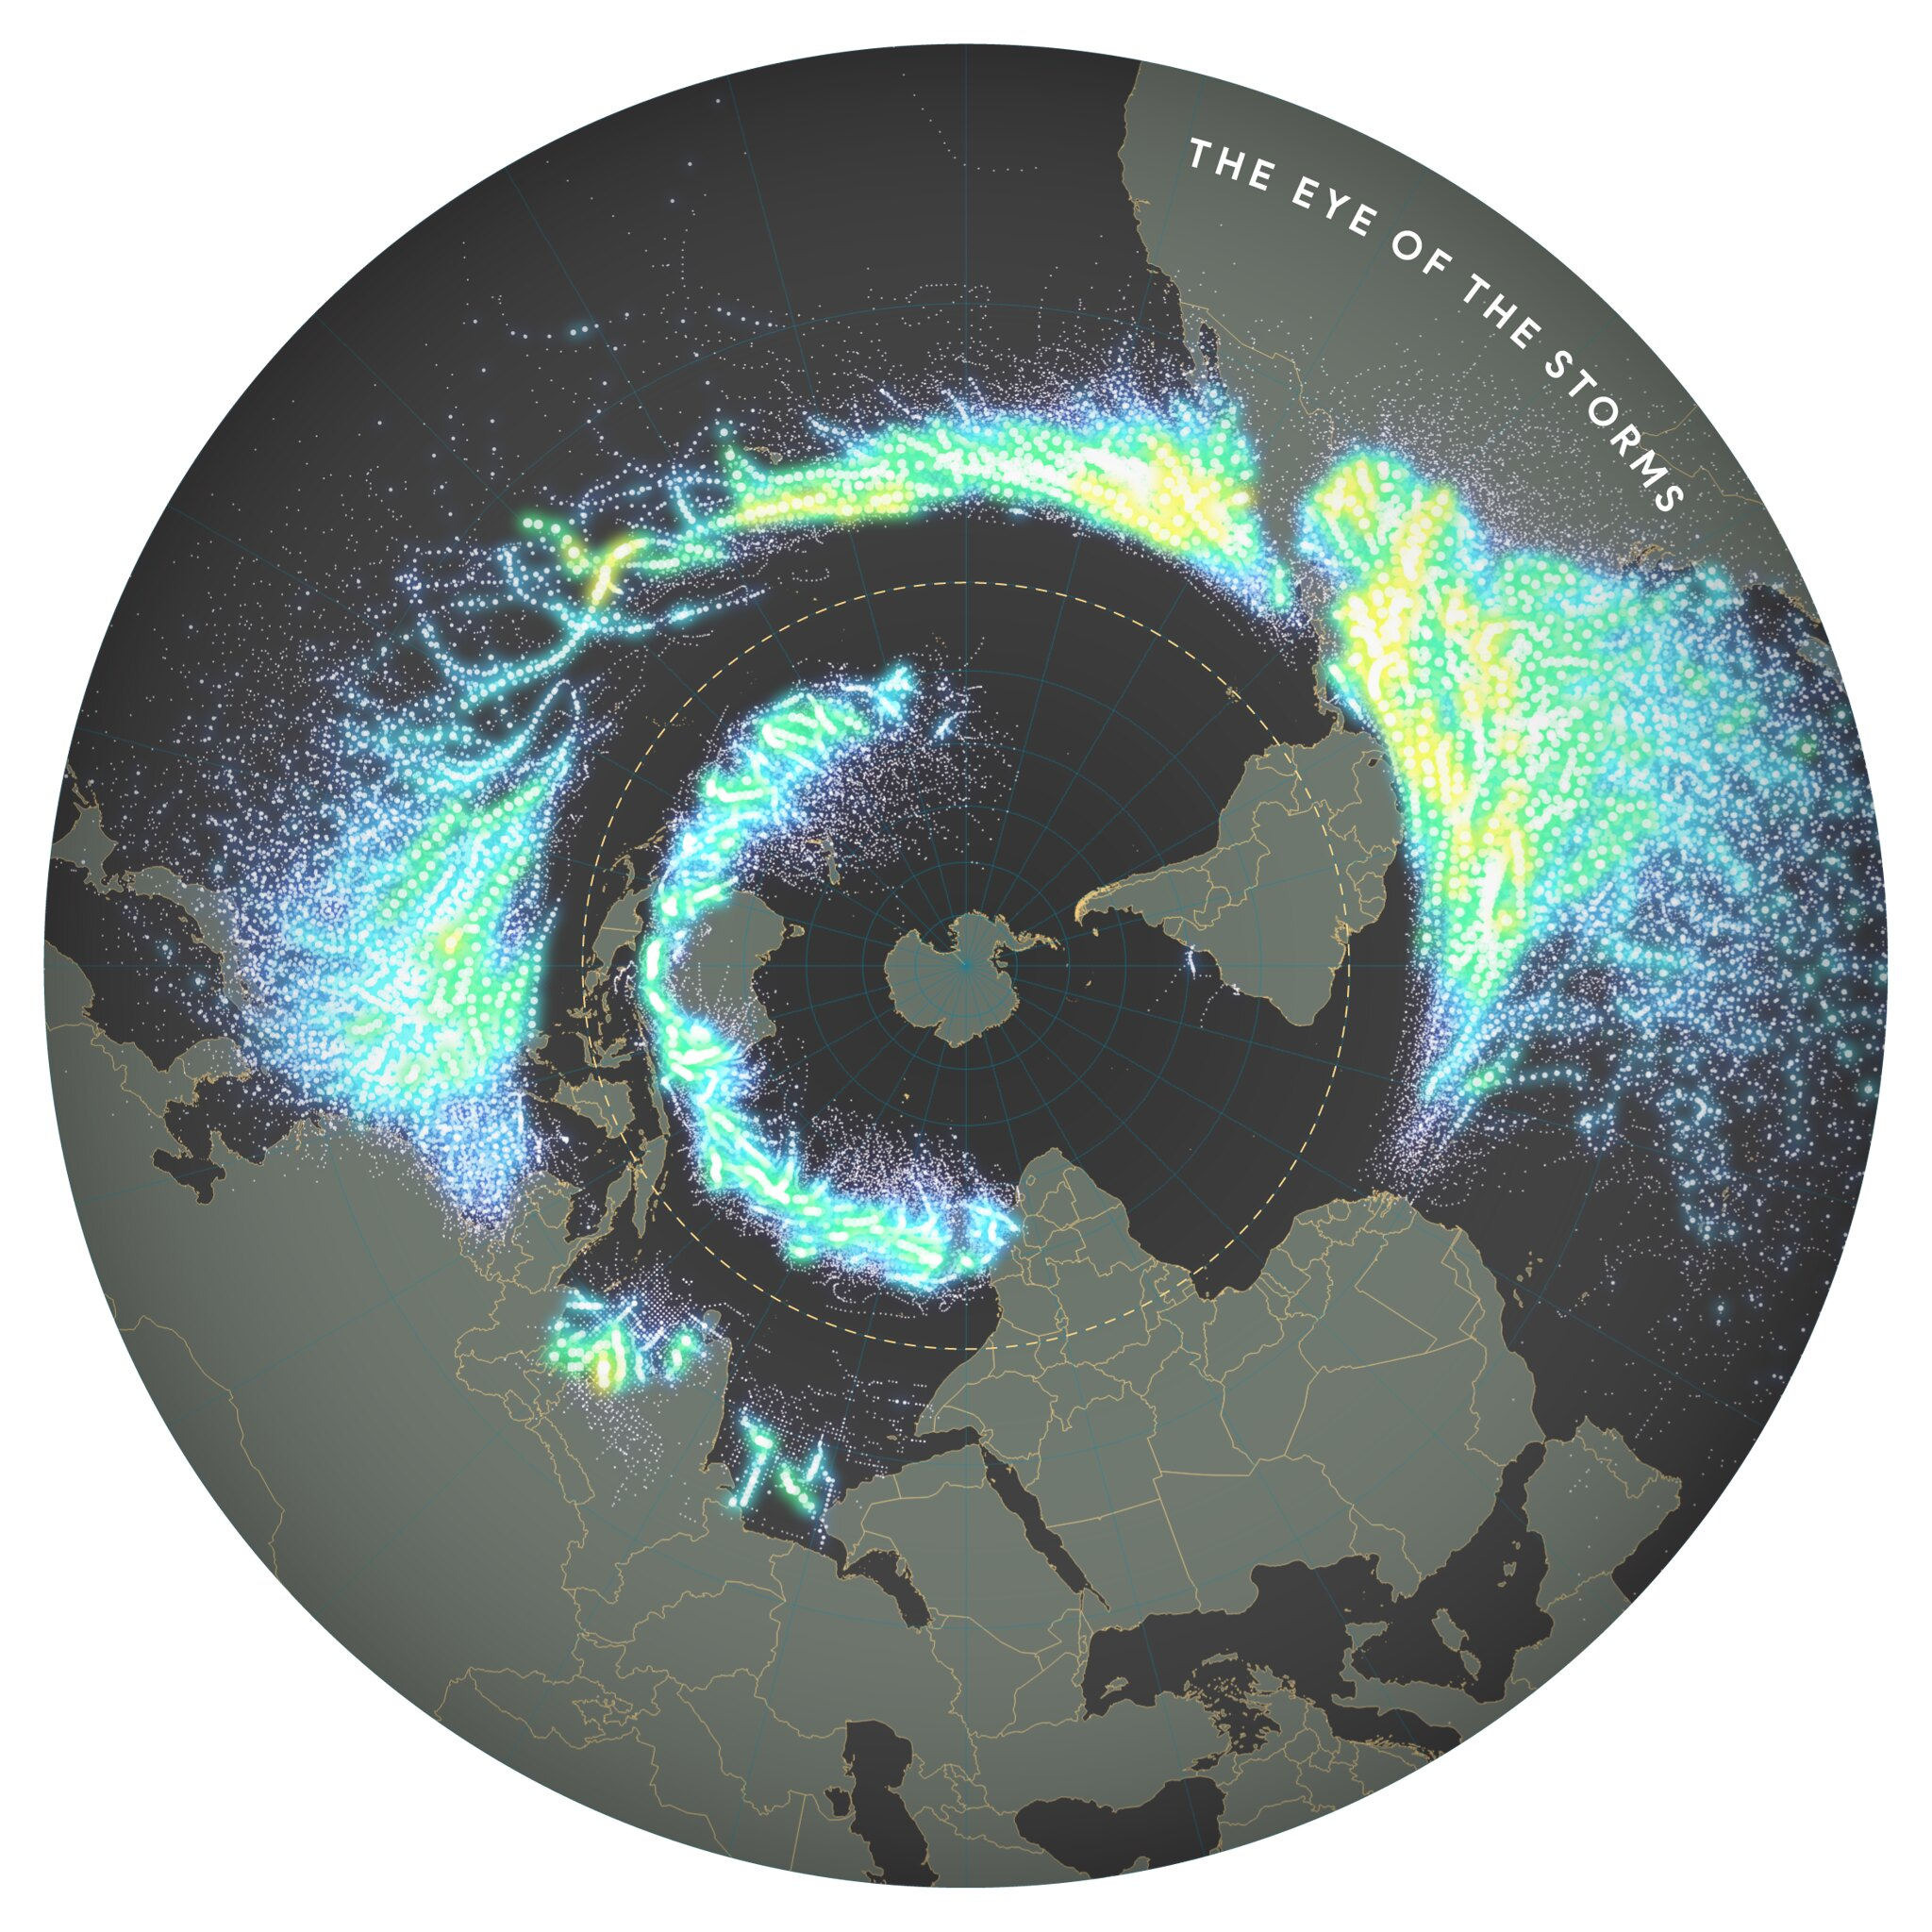
\includegraphics{media/modulo1/sample-2.jpg}
\caption{Dados de rastreamento de tempestade entre 1851 a 2020}
\end{figure}

Este próximo (\url{https://flic.kr/p/FA9TiR}) é um mapa da Ilha Kerguelen, feito por Heinrich Lingnau Schneider.

\begin{figure}
\centering
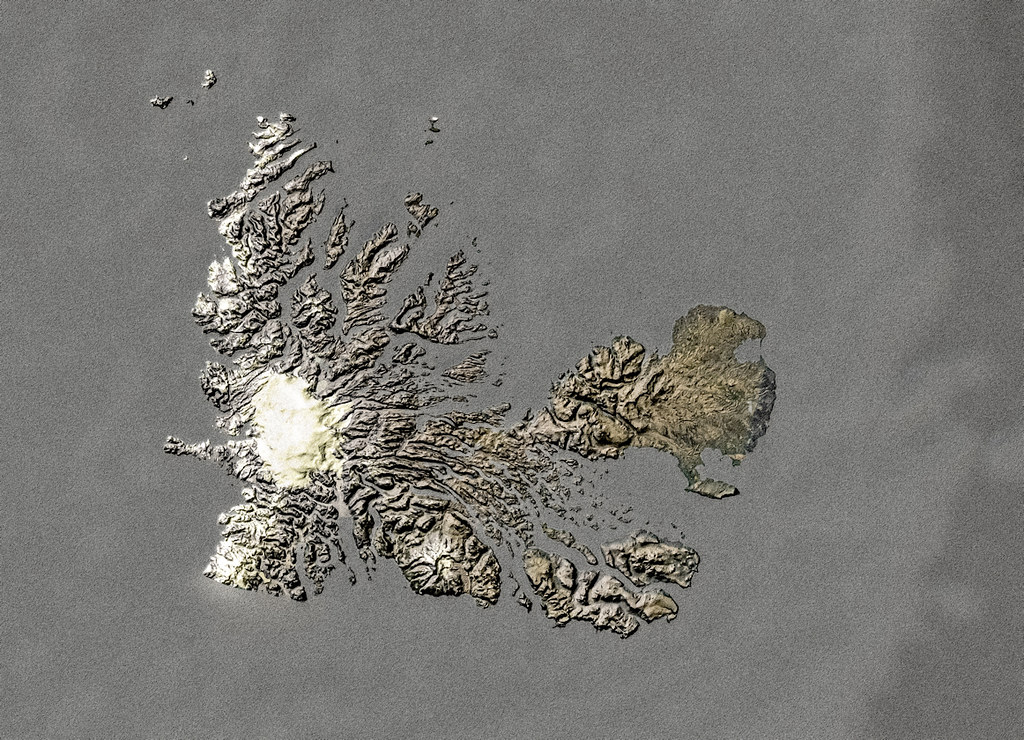
\includegraphics{media/modulo1/sample-3.jpg}
\caption{Mapa da Ilha Kerguelen}
\end{figure}

Este último (\href{https://flic.kr/p/v2kqVzsg}{https://flic.kr/p/2kqVzsg}) é de tentativas de arremessos de quadra e pontos marcados por tentativa durante a temporada 81 do Torneio de Basquete Masculino UAAP em as Filipinas por Ben Hur Pintor.

\begin{figure}
\centering
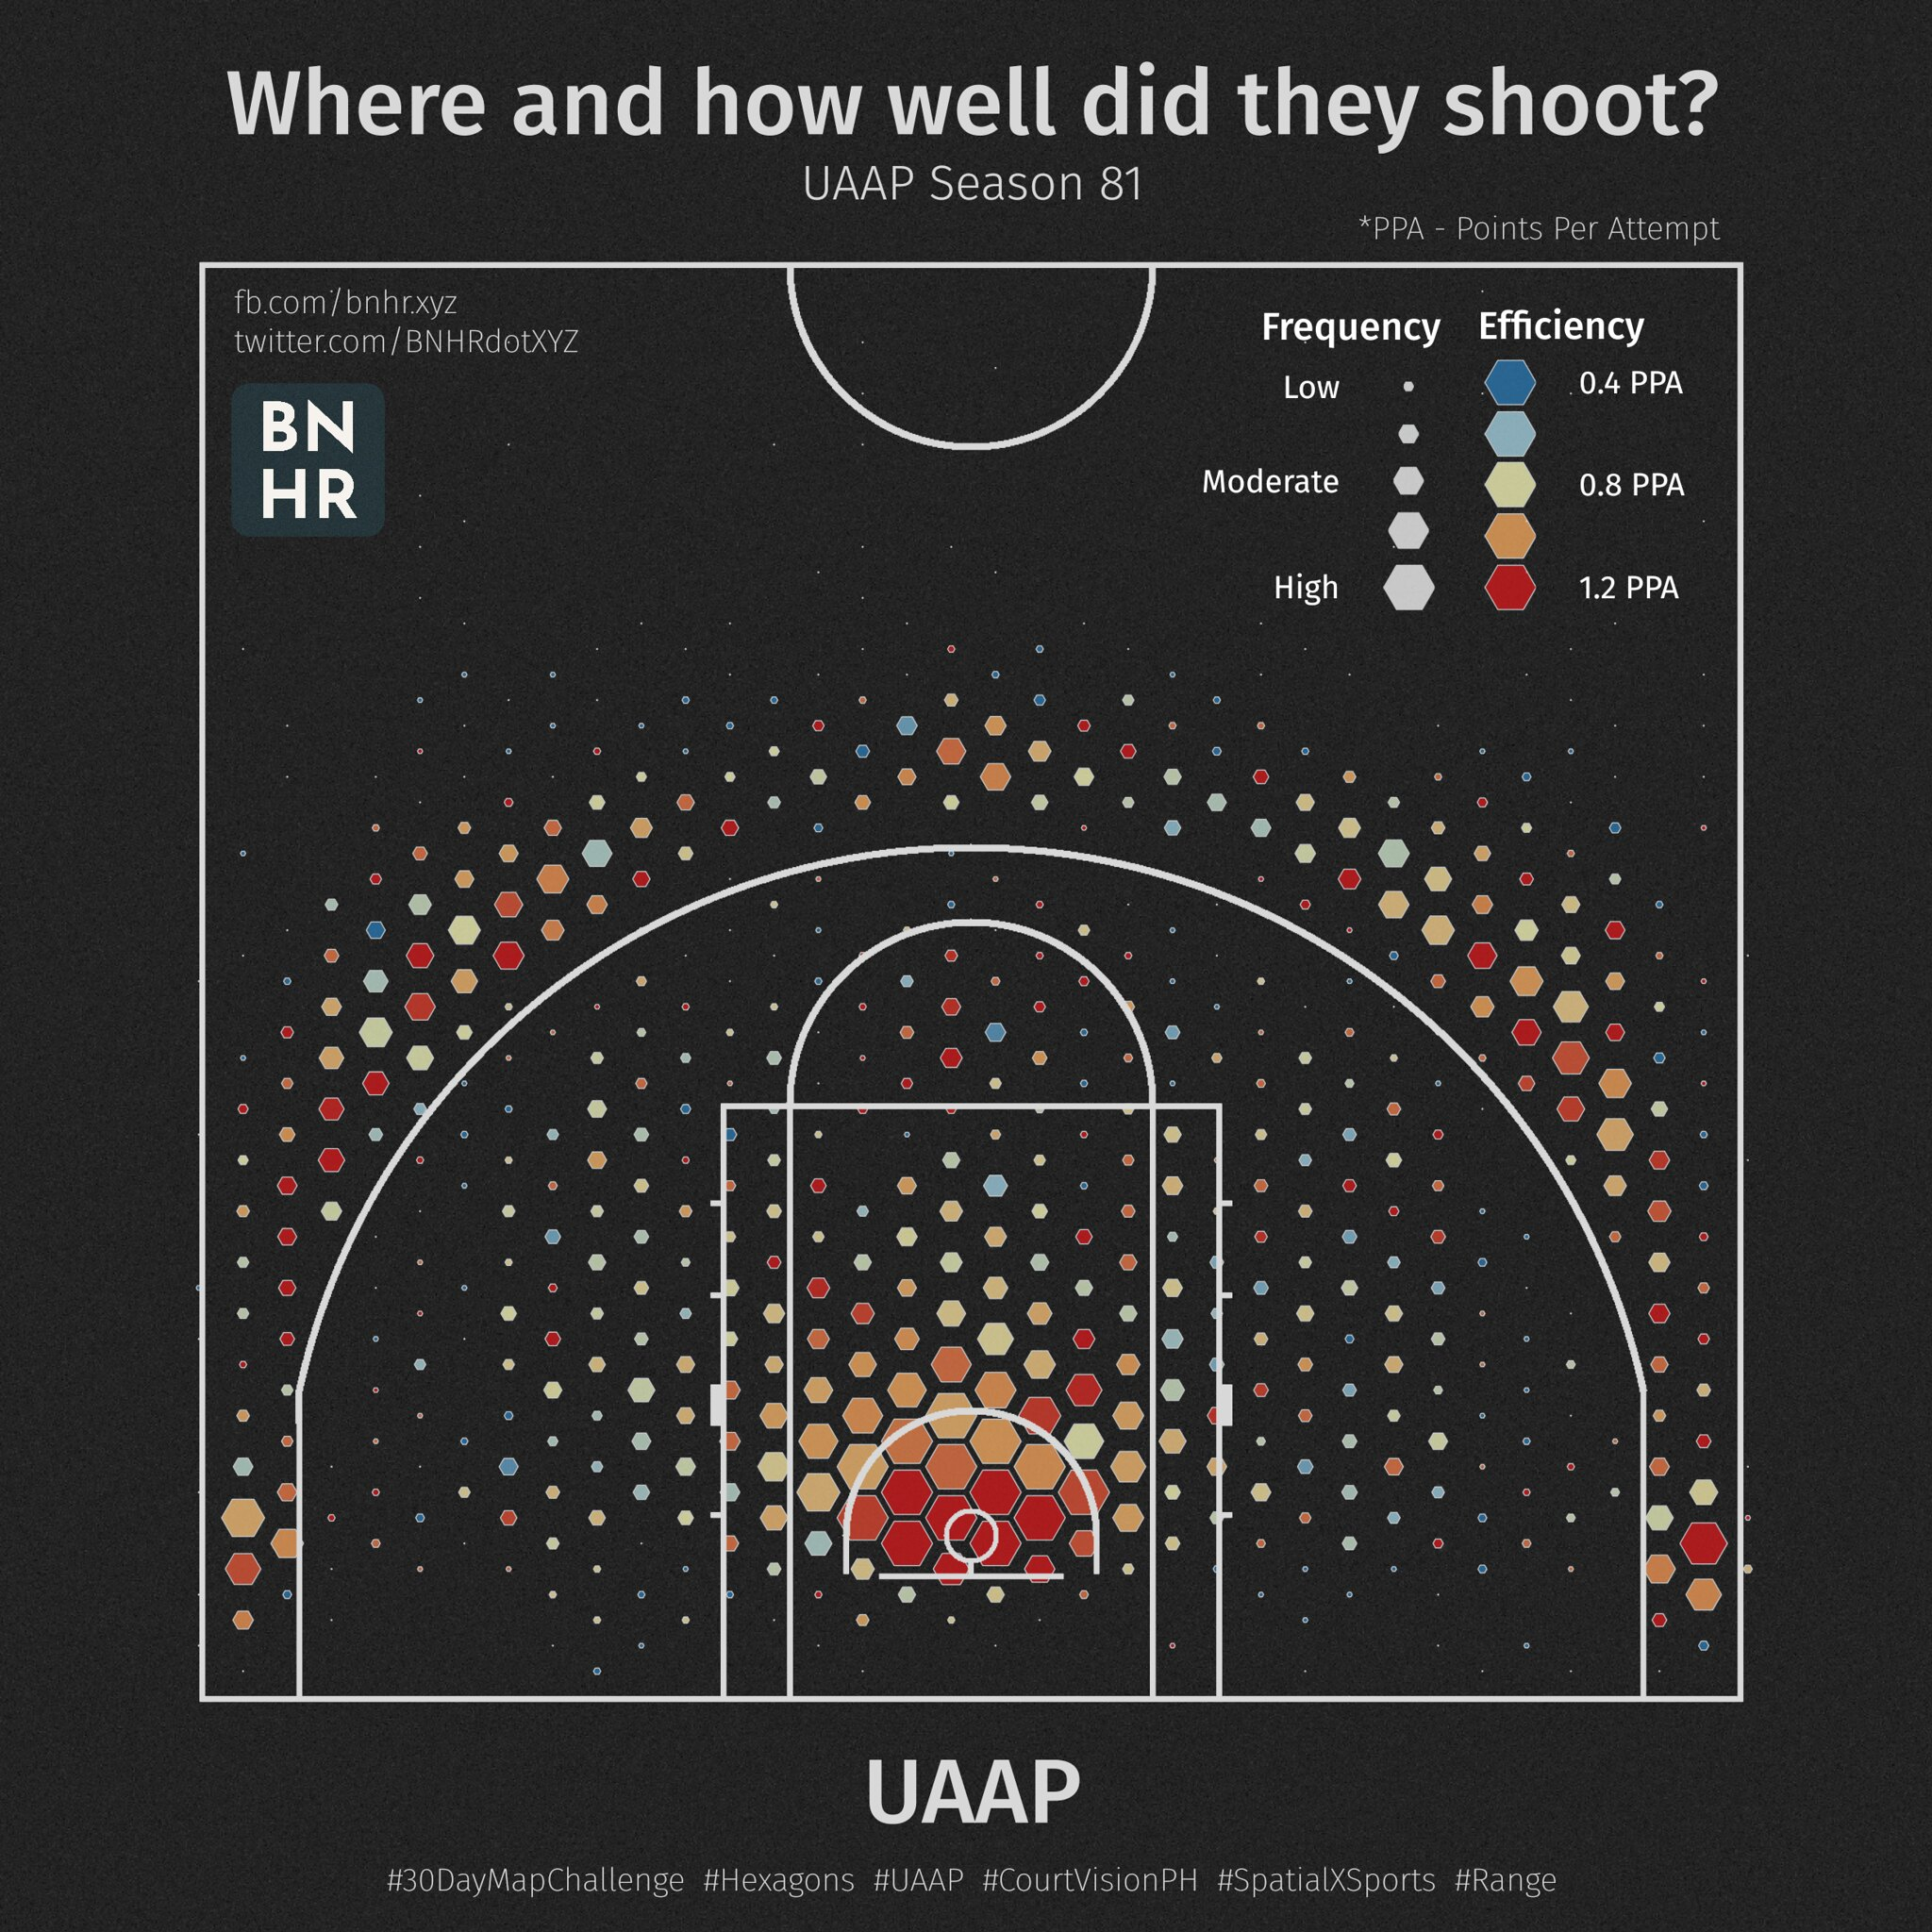
\includegraphics{media/modulo1/sample-4.jpg}
\caption{Tentativas de arremessos de quadra e pontos marcados na temporada 81 do UAAP}
\end{figure}

O que todos esses mapas têm em comum? Todos eles foram feitos usando o QGIS.

\hypertarget{detalhamento-dos-conceitos}{%
\section{Detalhamento dos conceitos}\label{detalhamento-dos-conceitos}}

Os mapas mostrados acima foram todos criados no QGIS (\url{https://qgis.org/en/site/}), um Sistema de Informação Geográfica (SIG, ou GIS) gratuito e de código aberto. O QGIS pode ser usado com todos os tipos de dados espaciais (como dados de basquete no último exemplo) e não apenas com dados geoespaciais relacionados à Terra.

As pessoas são capazes de criar mapas maravilhosos e surpreendentes, como os exemplos acima, porque o QGIS é gratuito, de código aberto e possui recursos poderosos de gerenciamento de dados, análise e apresentação.

\hypertarget{conteuxfado-principal-1}{%
\section{Conteúdo principal}\label{conteuxfado-principal-1}}

\hypertarget{tuxedtulo-da-fase-1-introduuxe7uxe3o-ao-qgis-e-uxe0-interface-do-qgis}{%
\subsection{Título da fase 1: Introdução ao QGIS e à interface do QGIS}\label{tuxedtulo-da-fase-1-introduuxe7uxe3o-ao-qgis-e-uxe0-interface-do-qgis}}

\hypertarget{o-que-uxe9-o-qgis}{%
\subsubsection{\texorpdfstring{\textbf{O que é o QGIS}}{O que é o QGIS}}\label{o-que-uxe9-o-qgis}}

\textbf{QGIS}, conhecido como Quantum GIS antes de seu lançamento 2.X, é um Sistema de Informação Geoespacial (GIS) maduro, multiplataforma, gratuito e de código aberto.

É um GIS de nível enterprise que possui recursos para coletar, armazenar, analisar, apresentar e gerenciar dados espaciais e não espaciais. Ele também se integra bem com outras tecnologias geoespaciais existentes e serve como parte integrante de qualquer pilha (stack) FOSS4G (Software Livre e de Código Aberto para Geoespacial).

Por ser multiplataforma, o QGIS pode ser executado em GNU / Linux, macOS, Windows e até mesmo Android.

\hypertarget{ciclo-de-lanuxe7amento-e-versuxf5es}{%
\subsubsection{\texorpdfstring{\textbf{Ciclo de lançamento e versões}}{Ciclo de lançamento e versões}}\label{ciclo-de-lanuxe7amento-e-versuxf5es}}

Os lançamentos e o desenvolvimento do QGIS seguem um cronograma / roteiro baseado no tempo (\href{https://www.qgis.org/en/site/\%20getinvolved\%20/\%20development\%20/\%20roadmap.html}{https://www.qgis.org/en/site/getinvolved/development/roadmap.html}).

Uma versão do QGIS é especificada por três números (X.Y.Z). Por exemplo, QGIS 3.16.4.

\begin{itemize}
\tightlist
\item
  X refere-se à versão principal. Neste caso, QGIS 3.
\item
  Y refere-se à versão de lançamento. Neste caso, a versão 16. As versões de lançamento são sempre números pares, pois os números ímpares são reservados para versões de desenvolvimento.
\item
  Z refere-se ao Point Release (PR) dessa versão. Para 3.16.4, isso significa que é o quarto ponto de lançamento da versão 3.16.
\end{itemize}

Existem três ramificações (ou branches) principais do QGIS que os usuários podem instalar. Estas são a ramificação \textbf{Long Term Release (LTR)}, a ramificação \textbf{Latest Release (LR)} e a ramificação \textbf{Development (Nightly)}.

\begin{itemize}
\tightlist
\item
  \textbf{Long Term Release (LTR)} tem esse nome porque é mantido e recebe correções de bug até o próximo LTR ser lançado. Atualmente, isso significa um (1) ano. Em fevereiro de 2021, o LTR atual é 3.16.4. Está programado para ser substituído pelo QGIS 3.22.4 em fevereiro de 2022.
\item
  \textbf{Última versão (LR)} refere-se a versão de lançamento do QGIS que contém os recursos mais recentes ou mais recentes. Um novo LR é lançado a cada quatro (4) meses. Por exemplo, um novo LR 3,18 foi lançado em fevereiro de 2021. O próximo LR (3.20) será lançado 4 meses a partir de agora, ou seja, em junho de 2021. Atualmente, cada terceiro LR se torna o próximo LTR. Por exemplo, o LTR de fevereiro de 2021 é a versão 3.16. O terceiro LR de 3.16 é 3.22, portanto, o próximo LTR será baseado na versão de lançamento 3.22.
\item
  \textbf{Development / Nightly} é baseado na versão mais recente do código-fonte QGIS, mas é útil se você deseja testar, depurar ou ajudar no desenvolvimento do QGIS.
\end{itemize}

Então, qual versão você deve usar? Depende. Se você precisa de uma versão que é mantida por mais tempo e não precisa necessariamente de novos recursos à medida que são lançados, a versão LTR pode ser a versão para você. Se você precisa dos recursos mais recentes e não se importa em fazer uma atualização a cada poucos meses, a versão LR pode ser ideal para você. Às vezes, também é bom dar uma olhada nas versões de desenvolvimento ou noturnas, especialmente se você estiver curioso ou animado com os próximos recursos do QGIS.

Para obter mais informações, visite: \href{https://bnhr.xyz/2020/10/26/\%20about-qgis-versions-release-cycle-english.html}{https://bnhr.xyz/2020/10/26/about-qgis-versions-release-cycle-english.html}

\hypertarget{exemplos-de-mapas-qgis}{%
\subsubsection{\texorpdfstring{\textbf{Exemplos de mapas QGIS}}{Exemplos de mapas QGIS}}\label{exemplos-de-mapas-qgis}}

\begin{figure}
\centering
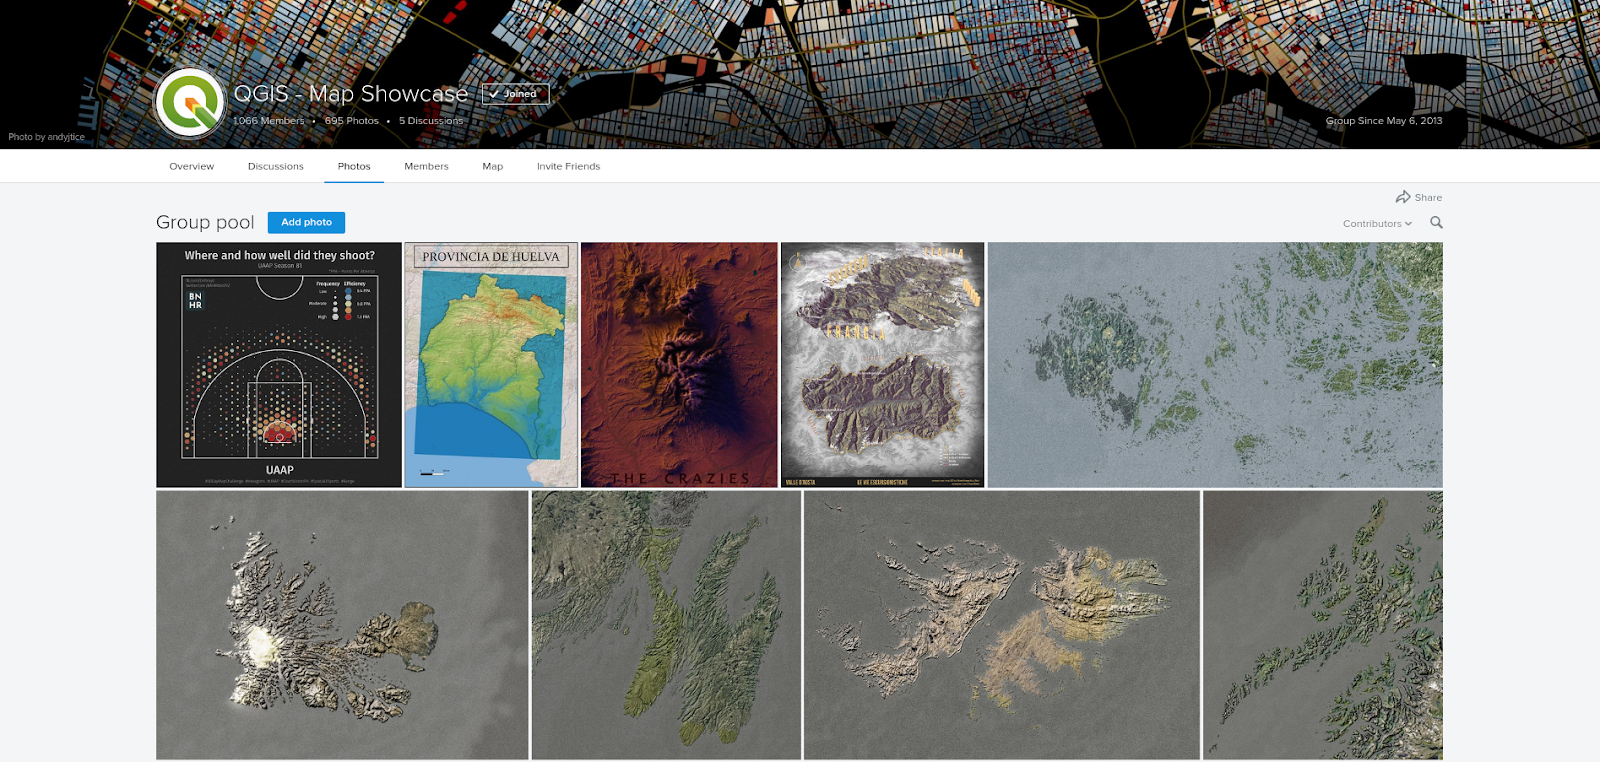
\includegraphics{media/modulo1/qgis-map-showcase.png}
\caption{QGIS Map Showcase}
\end{figure}

Figura 1.1. Demonstração do mapa QGIS

Para mais mapas criados com o QGIS, visite: \href{https://www.flickr.com/groups/2244553@N22/\%20piscina/com/50355460063/}{https://www.flickr.com/groups/2244553@N22/pool/with/50355460063/}

\hypertarget{instalando-o-qgis}{%
\subsubsection{\texorpdfstring{\textbf{Instalando o QGIS}}{Instalando o QGIS}}\label{instalando-o-qgis}}

QGIS é multiplataforma e funciona em Linux, Windows e macOS. Sendo de código aberto, você pode construir e instalar o QGIS a partir de seu código-fonte, disponível em \url{https://github.com/qgis/QGIS/}.

Instaladores e instruções de instalação também estão disponíveis em \url{https://qgis.org/en/site/forusers/download.html} ou \href{https://qgis.org/en/site/forusers/alldownloads.html}{https: //qgis.org/en/site/forusers/alldownloads.html}.

Para \textbf{Linux (ou GNU / Linux)}, o QGIS geralmente está disponível no gerenciador de pacotes de sua distribuição. Para usuários Debian / Ubuntu, o QGIS tem repositórios para os ramos LR, LTR e Desenvolvimento (Development), bem como versões do QGIS com dependências do PPA ubuntugis-unstable. O QGIS também está disponível como pacote Flatpak ou no Conda.

Para \textbf{Windows}, os usuários podem escolher entre o instalador de rede OSGeo4W ou os instaladores independentes. Há um instalador independente para a versão LTR e LR.

Os instaladores autônomos são os mais fáceis de instalar e são recomendados para iniciantes. Várias versões do QGIS podem ser instaladas em seu computador ao mesmo tempo. Isso significa que você pode ter ambas as versões QGIS 3.16 e 3.18 instaladas.

O OSGeo4W Network Installer é um pouco mais avançado e complexo do que os instaladores autônomos, mas também oferece a capacidade de atualizar e atualizar sua versão do QGIS no local, o que significa que você não precisará desinstalar uma versão mais antiga se quiser instalar um mais novo.

Em alguns casos, você precisará de direitos de administrador para instalar o QGIS, portanto, se estiver instalando em um computador onde o seu usuário não possui direitos de administrador, pode ser necessário pedir ao seu administrador de TI ou escritório para instalar o QGIS para você.

A instalação no Windows também vem com QGIS com GRASS (outro GIS Livre e de Código Aberto).

Observe que o QGIS está \href{https://blog.qgis.org/2020/10/15/phasing-out-32-bit-support-in-qgis/}{removendo lentamente o suporte de 32 bits para Windows}, então é melhor para instalar o QGIS em um computador que executa um sistema operacional de 64 bits.

Para o \textbf{macOS}, existem instaladores oficiais ``All-in-one'' assinados para macOS High Sierra (10.13) e mais recentes. O QGIS ainda não foi autenticado conforme exigido pelas regras de segurança do macOS Catalina (10.15). Na primeira inicialização, clique com o botão direito no ícone do aplicativo QGIS, segure a tecla Option e escolha Abrir.

\hypertarget{partes-da-interface-do-qgis}{%
\subsubsection{\texorpdfstring{\textbf{Partes da interface do QGIS}}{Partes da interface do QGIS}}\label{partes-da-interface-do-qgis}}

Depois de instalar o QGIS, você pode executá-lo ou abri-lo como faria com qualquer programa em seu computador. Ao abrir o QGIS, você será saudado com a Interface do Usuário (IU, ou UI em inglês) padrão que se parecerá com a abaixo.

\begin{figure}
\centering
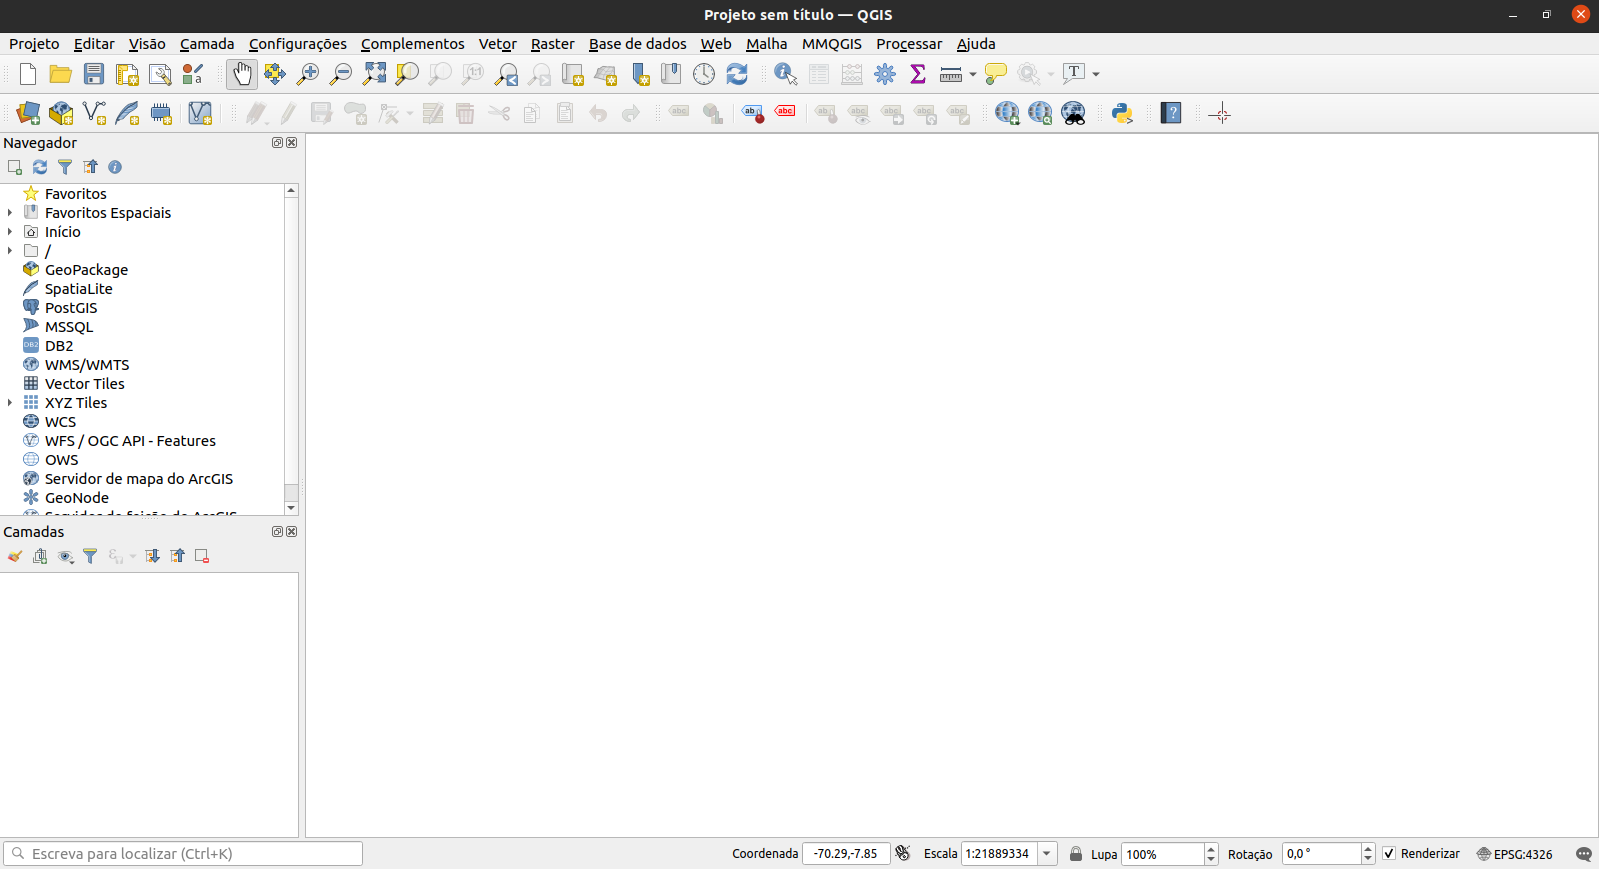
\includegraphics{media/modulo1/qgis-interface.png}
\caption{A interface QGIS}
\end{figure}

Figura 1.2. A interface QGIS em uma nova instalação

Existem seis partes principais da interface de usuário do QGIS - barra de menu, tela do mapa, barra de ferramentas, painéis, barra de status e localizador.

No centro da interface está uma tela de mapa. Painéis e barras de ferramentas podem ser posicionados em torno dessa tela. Os painéis também podem ser acoplados para criar um painel com várias abas. Existem também outras partes da interface, como a interface Python, janelas de complemento, etc.

\textbf{Barra de menus} - a barra de menus é um menu hierárquico simples que fornece acesso às funções e comandos do QGIS. Geralmente está localizado na parte superior da interface.

\textbf{Tela do mapa} - a tela do mapa é onde as camadas carregadas no QGIS são mostradas. Este é também o local onde os filtros, seleções, e simbologias criadas pelo usuário são refletidas. Mais de uma tela de mapa pode estar presente a qualquer momento. Um usuário pode aplicar zoom, panorâmica e até mesmo girar a tela do mapa. Uma tela de mapa também pode mostrar dados 3D.

\textbf{Barras de ferramentas} - as barras de ferramentas mostram botões de acesso fácil aos comandos, recursos, complementos do QGIS. Eles podem ser movidos e encaixados na tela do mapa. A lista de barras de ferramentas pode ser encontrada, ativada e desativada na barra de menus em \textbf{Exibir ‣ Barras de ferramentas}. Exemplos de barras de ferramentas são a barra de ferramentas de atributos e a barra de ferramentas de digitalização.

\textbf{Painéis} - os painéis são semelhantes às barras de ferramentas, mas, em vez de botões, fornecem uma interface para funções e recursos mais complexos. O painel de camadas e o painel do navegador são dois exemplos. Semelhante às barras de ferramentas, eles podem ser movidos e encaixados na tela do mapa. A lista de painéis pode ser encontrada, ativada e desativada na barra de menus em \textbf{Exibir ‣ Painéis}.

\textbf{Barra de status} - a barra de status é comumente encontrada na parte inferior da interface e mostra informações relevantes, como CRS, escala, notificações, etc.

\textbf{Barra Localizadora} - a barra Localizadora é encontrada no canto inferior esquerdo da interface do QGIS. Ele permite que o usuário acesse facilmente camadas, campos, algoritmos de processamento e outras funcionalidades no QGIS. Este é um dos recursos mais poderosos do QGIS.

\begin{figure}
\centering
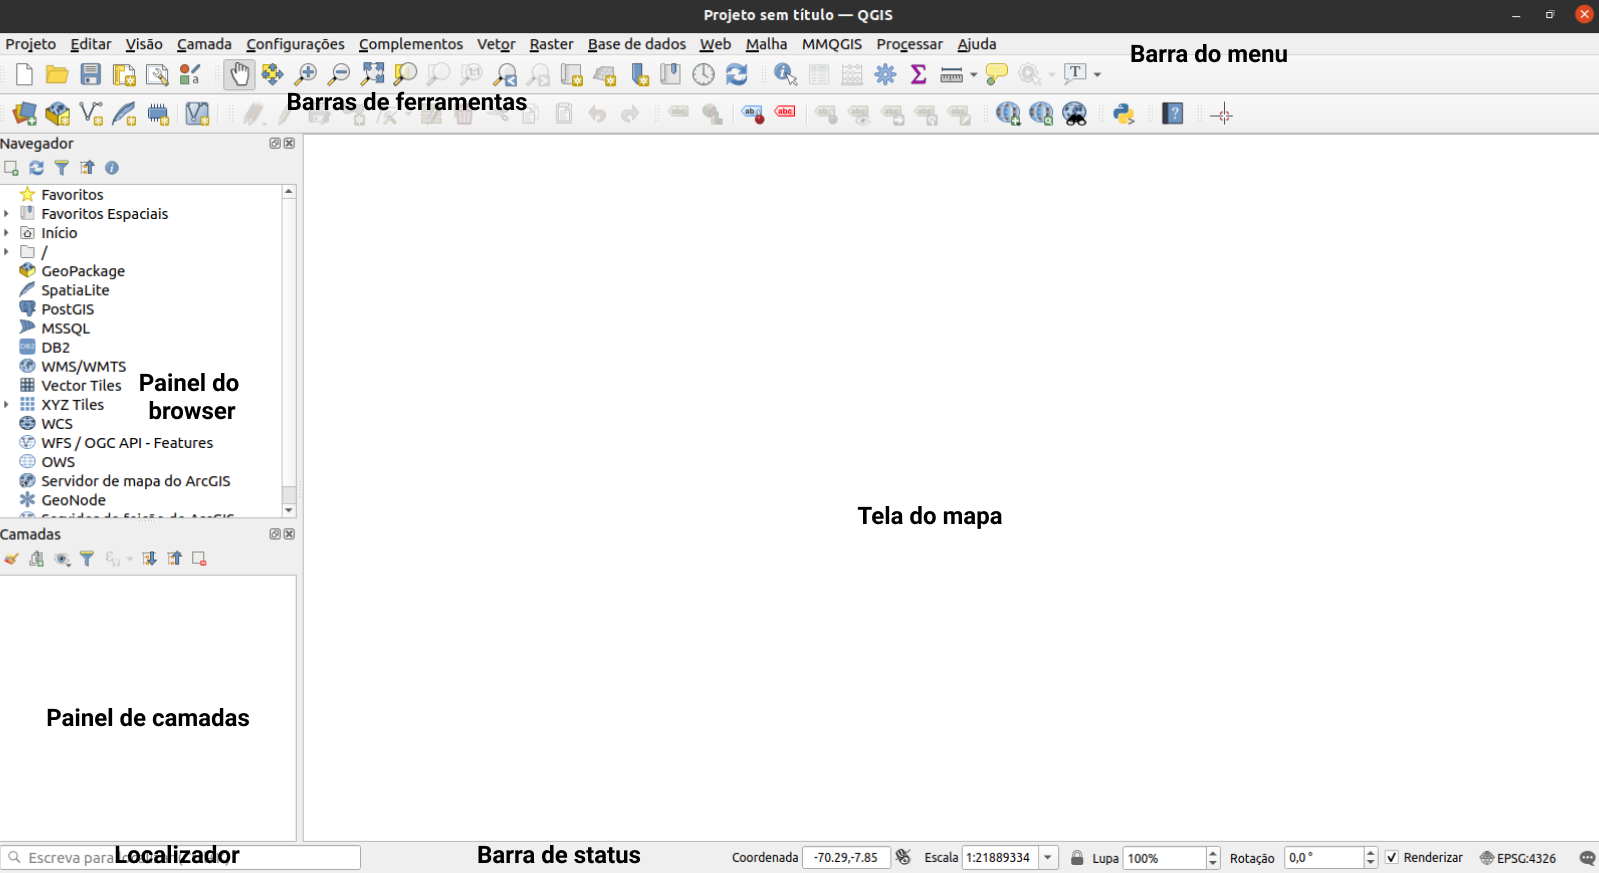
\includegraphics{media/modulo1/qgis-interface-parts.png}
\caption{Partes da interface QGIS}
\end{figure}

Figura 1.3. Partes da interface QGIS

Uma das belezas do QGIS é a personalização ele que oferece aos seus usuários. Essa personalização começa com a interface do usuário. Ao editar algumas configurações e mover algumas partes da interface, você pode ter um QGIS semelhante a este abaixo:

\begin{figure}
\centering
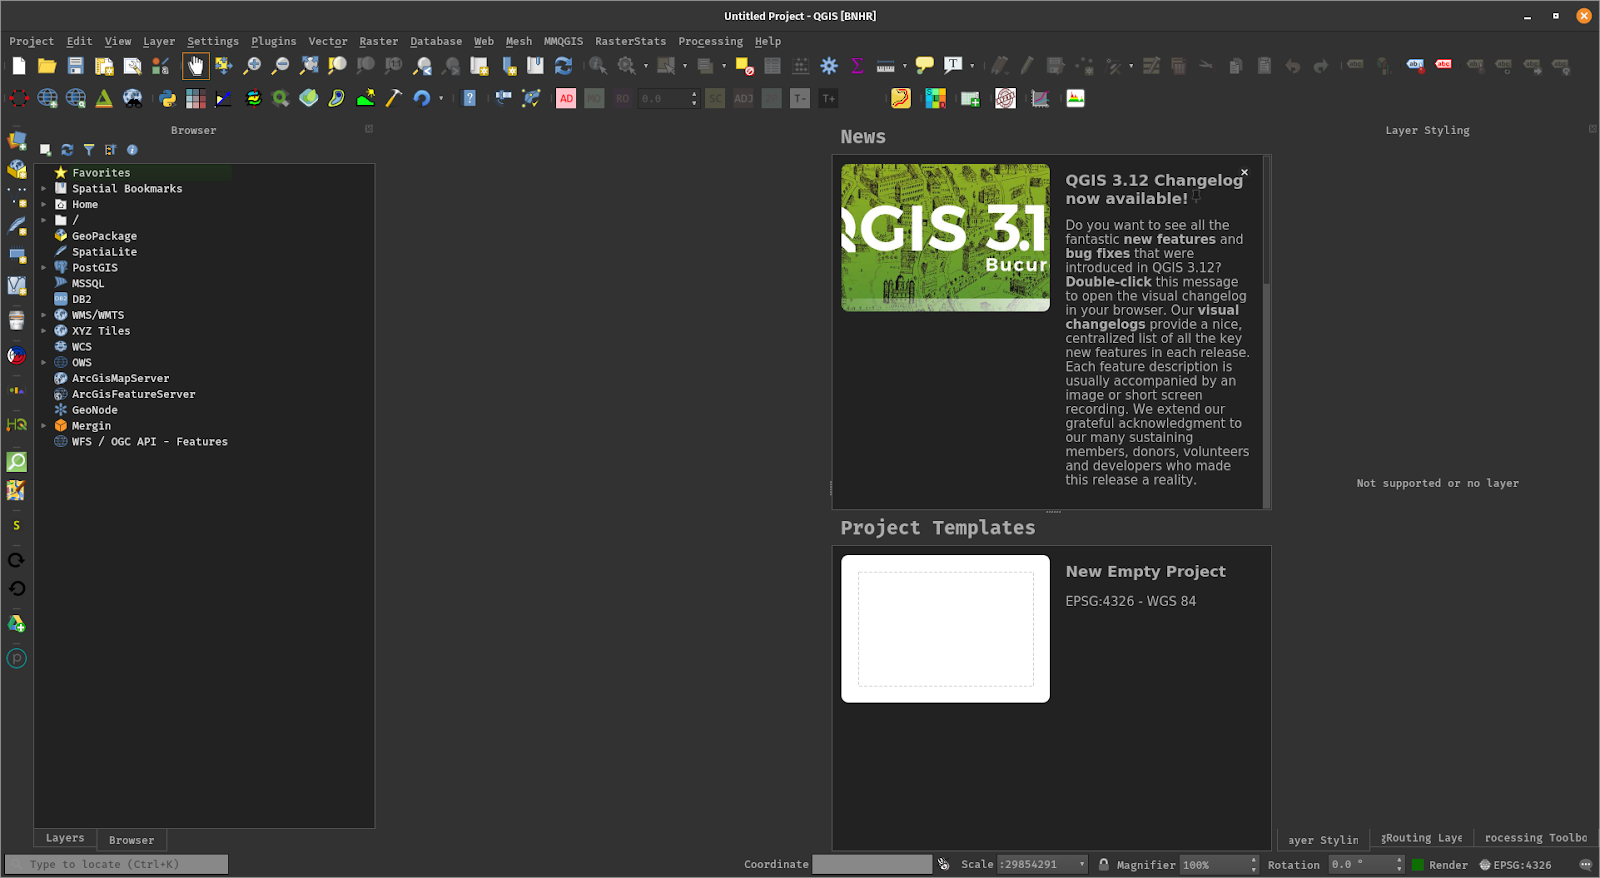
\includegraphics{media/modulo1/qgis-interface-custom.png}
\caption{Interface QGIS com algumas personalizações}
\end{figure}

Figura 1.4. A interface QGIS com algumas personalizações

\hypertarget{tutorial-exercuxedcio-1-mudando-a-aparuxeancia-e-layout-da-interface-qgis}{%
\subsubsection{\texorpdfstring{\textbf{Tutorial / Exercício 1: Mudando a aparência e layout da interface QGIS}}{Tutorial / Exercício 1: Mudando a aparência e layout da interface QGIS}}\label{tutorial-exercuxedcio-1-mudando-a-aparuxeancia-e-layout-da-interface-qgis}}

\begin{enumerate}
\def\labelenumi{\arabic{enumi}.}
\tightlist
\item
  Abra o \textbf{QGIS}
\item
  Clique no menu \textbf{Visão}
\end{enumerate}

\begin{figure}
\centering
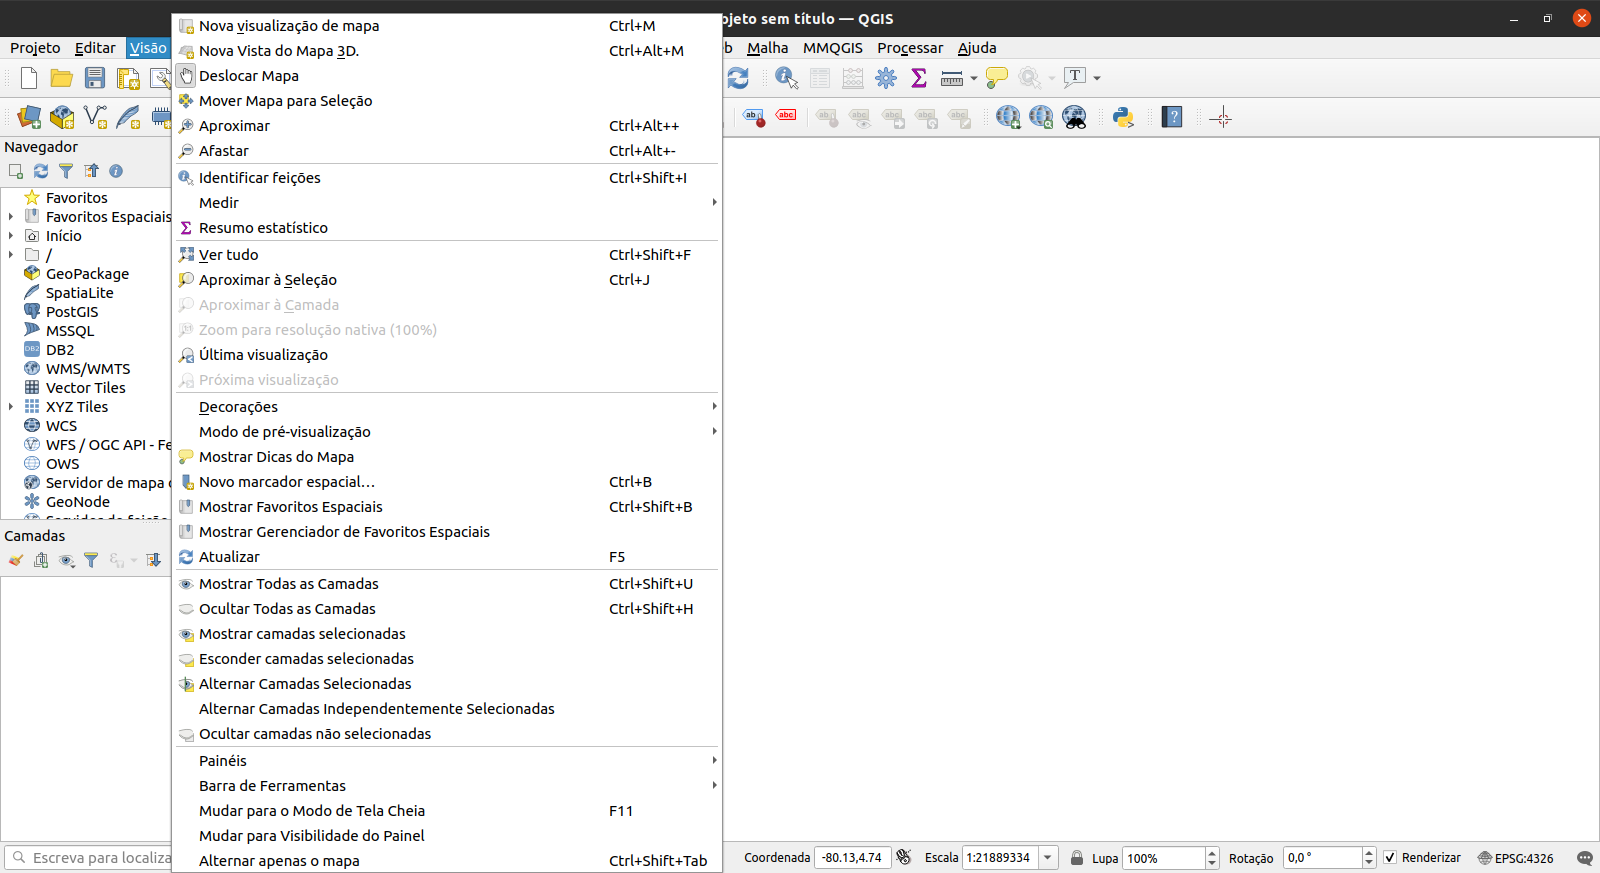
\includegraphics{media/modulo1/ex01-01.png}
\caption{Abra o QGIS e clique no menu Exibir}
\end{figure}

\begin{enumerate}
\def\labelenumi{\arabic{enumi}.}
\setcounter{enumi}{2}
\tightlist
\item
  Observe o menu \textbf{Painéis}
\end{enumerate}

\begin{figure}
\centering
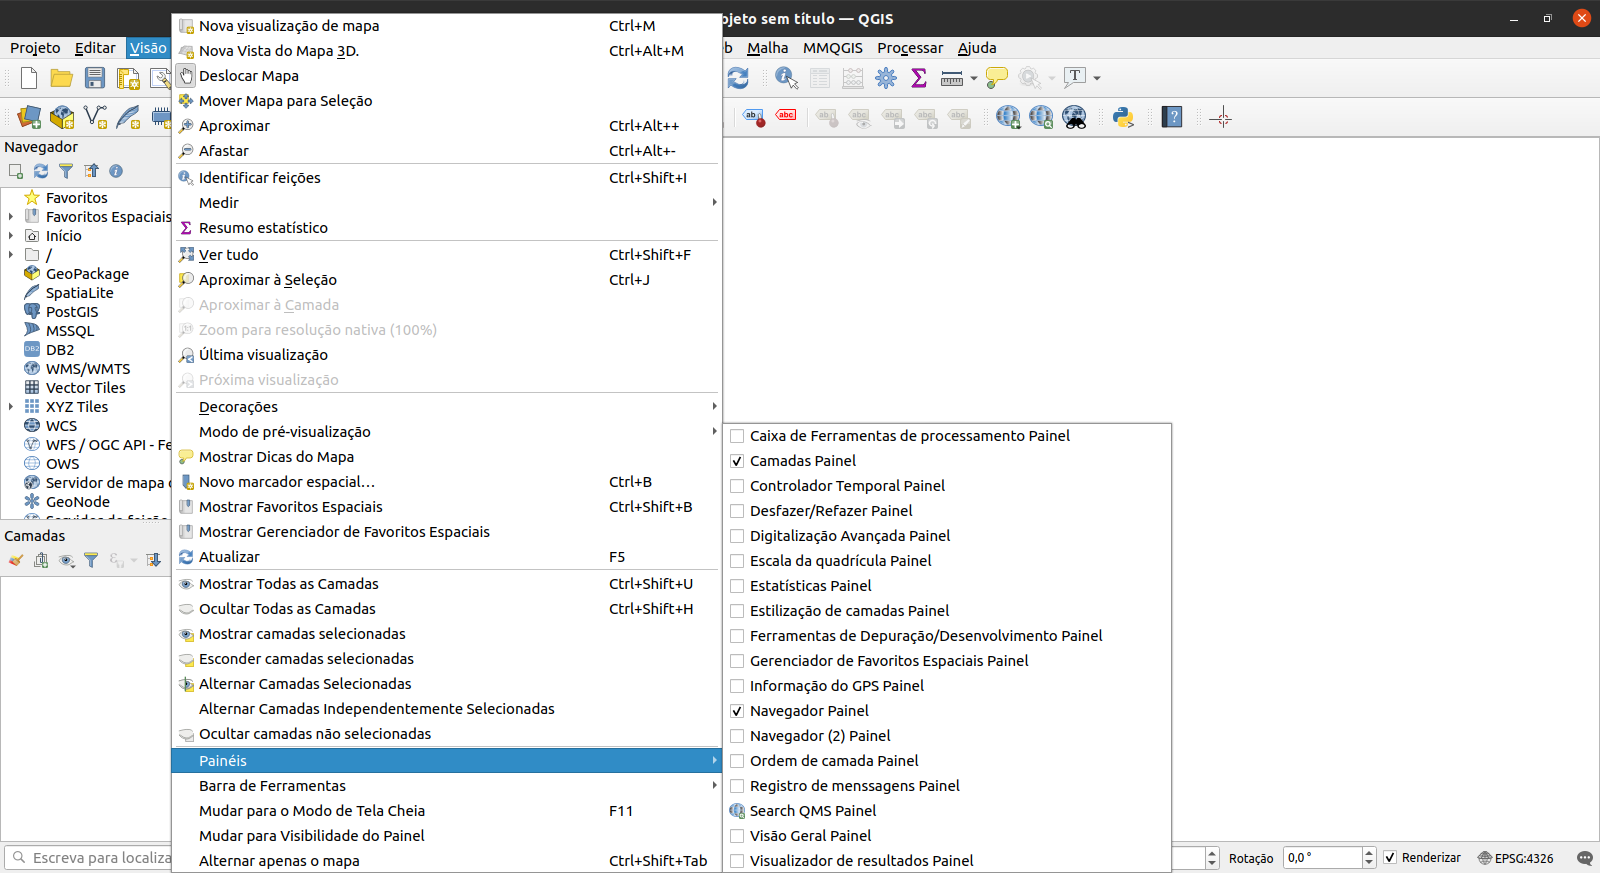
\includegraphics{media/modulo1/ex01-02.png}
\caption{Observe o menu Painéis}
\end{figure}

\begin{enumerate}
\def\labelenumi{\arabic{enumi}.}
\setcounter{enumi}{3}
\tightlist
\item
  Observe o menu \textbf{Barras de ferramentas}
\end{enumerate}

\begin{figure}
\centering
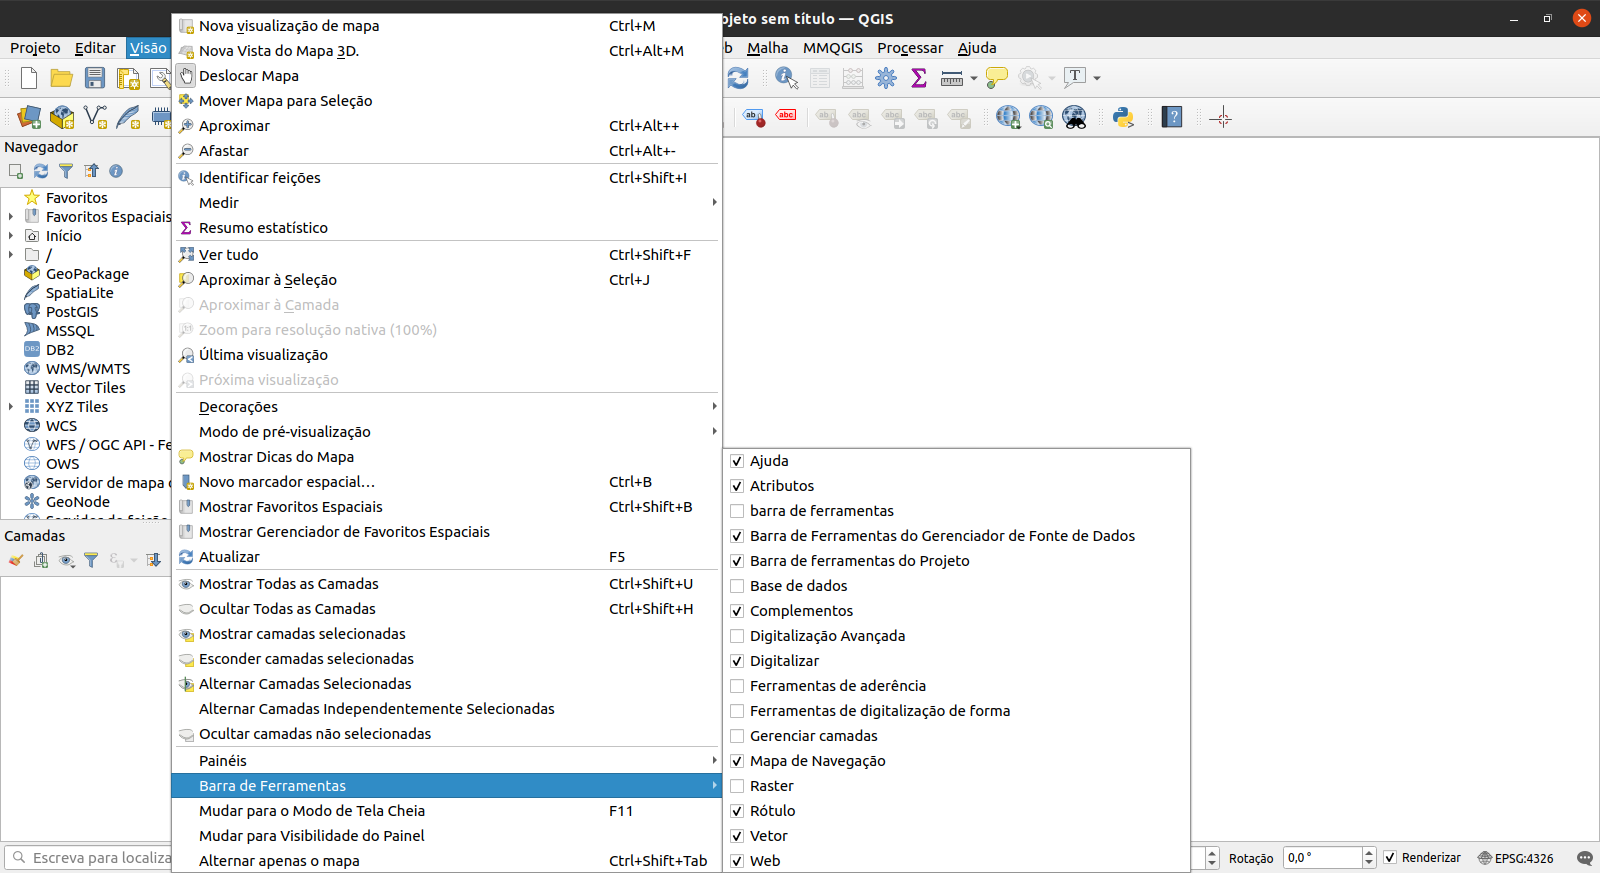
\includegraphics{media/modulo1/ex01-03.png}
\caption{Observe o menu Barras de ferramentas}
\end{figure}

\begin{enumerate}
\def\labelenumi{\arabic{enumi}.}
\setcounter{enumi}{4}
\tightlist
\item
  Selecione as \textbf{Barras de ferramentas} e \textbf{Painéis} que você deseja mostrar na interface do usuário. Alguns dos painéis úteis incluem \textbf{Estilização de camadas} e \textbf{Caixa de Ferramentas de Processamento}.
\item
  Mova as \textbf{Barras de Ferramentas} e \textbf{Painéis} para as posições que fizerem mais sentido para você
\end{enumerate}

\textbf{Resetando a interface QGIS}

Para redefinir sua tela para as configurações padrão, vá para \textbf{Configurações ‣ Opções ‣ Guia Sistema ‣ Configurações ‣ Botão Redefinir} e reinicie o QGIS.

\hypertarget{perguntas-do-questionuxe1rio-2}{%
\subsubsection{\texorpdfstring{\textbf{Perguntas do questionário}}{Perguntas do questionário}}\label{perguntas-do-questionuxe1rio-2}}

\begin{enumerate}
\def\labelenumi{\arabic{enumi}.}
\tightlist
\item
  Verdadeiro ou falso:

  \begin{enumerate}
  \def\labelenumii{\arabic{enumii}.}
  \tightlist
  \item
    Você pode ter várias telas de mapa - \textbf{\emph{Verdadeiro}}
  \item
    Você pode mostrar ou ocultar painéis e barras de ferramentas - \textbf{\emph{Verdadeiro}}
  \item
    Você só pode colocar painéis no lado esquerdo ou direito da tela do mapa - \textbf{\emph{Falso (você também pode colocar painéis acima ou abaixo da tela do mapa)}}
  \end{enumerate}
\end{enumerate}

\hypertarget{tuxedtulo-da-fase-2-complementos-complementos-qgis}{%
\subsection{Título da fase 2: Complementos (Complementos) QGIS}\label{tuxedtulo-da-fase-2-complementos-complementos-qgis}}

A capacidade de adicionar, criar e estender a funcionalidade do QGIS por meio de complementos (ou plug-ins) é um de seus recursos mais poderosos.

A partir do QGIS 3.16.3, existem mais de 700 complementos disponíveis para o usuário baixar e melhorar. Esses complementos variam do complexo ao simples.

Os complementos QGIS podem ser classificados como:

\begin{itemize}
\tightlist
\item
  \textbf{Complementos core} - integrado à sua versão do QGIS, não pode ser desinstalado
\item
  \textbf{Complementos externos} - manualmente instalados por meio de busca em um repositório externo (ou seja, QGIS Official Plugin Repository) ou através do código-fonte.
\end{itemize}

Os complementos podem ser instalados de três (3) maneiras:

\begin{enumerate}
\def\labelenumi{\arabic{enumi}.}
\tightlist
\item
  Através da caixa de diálogo Gerenciar e instalar complementos (\textbf{Complementos ‣ Gerenciar e instalar complementos})
\item
  Instalando do ZIP, que pode ser acessado na guia \textbf{Instalar do ZIP} na caixa de diálogo Gerenciar e instalar complementos.
\item
  Adicionando manualmente o código-fonte na pasta de complementos do seu perfil QGIS. Essa pasta geralmente pode ser encontrada em:

  \begin{enumerate}
  \def\labelenumii{\arabic{enumii}.}
  \tightlist
  \item
    \textbf{Linux}: .local/share/QGIS/QGIS3/profiles/default/python/plugins
  \item
    \textbf{Mac OS X}: Biblioteca/Aplicativo/Suporte/QGIS/QGIS3/profiles/default/python/plugins
  \item
    \textbf{Windows:} \texttt{C:\textbackslash{}Usuário\textbackslash{}\textless{}Nome\textgreater{}\textbackslash{}AppData\textbackslash{}Roaming\textbackslash{}QGIS\textbackslash{}QGIS3\textbackslash{}profiles\textbackslash{}default\textbackslash{}python\textbackslash{}plugins}
  \end{enumerate}
\end{enumerate}

\begin{figure}
\centering
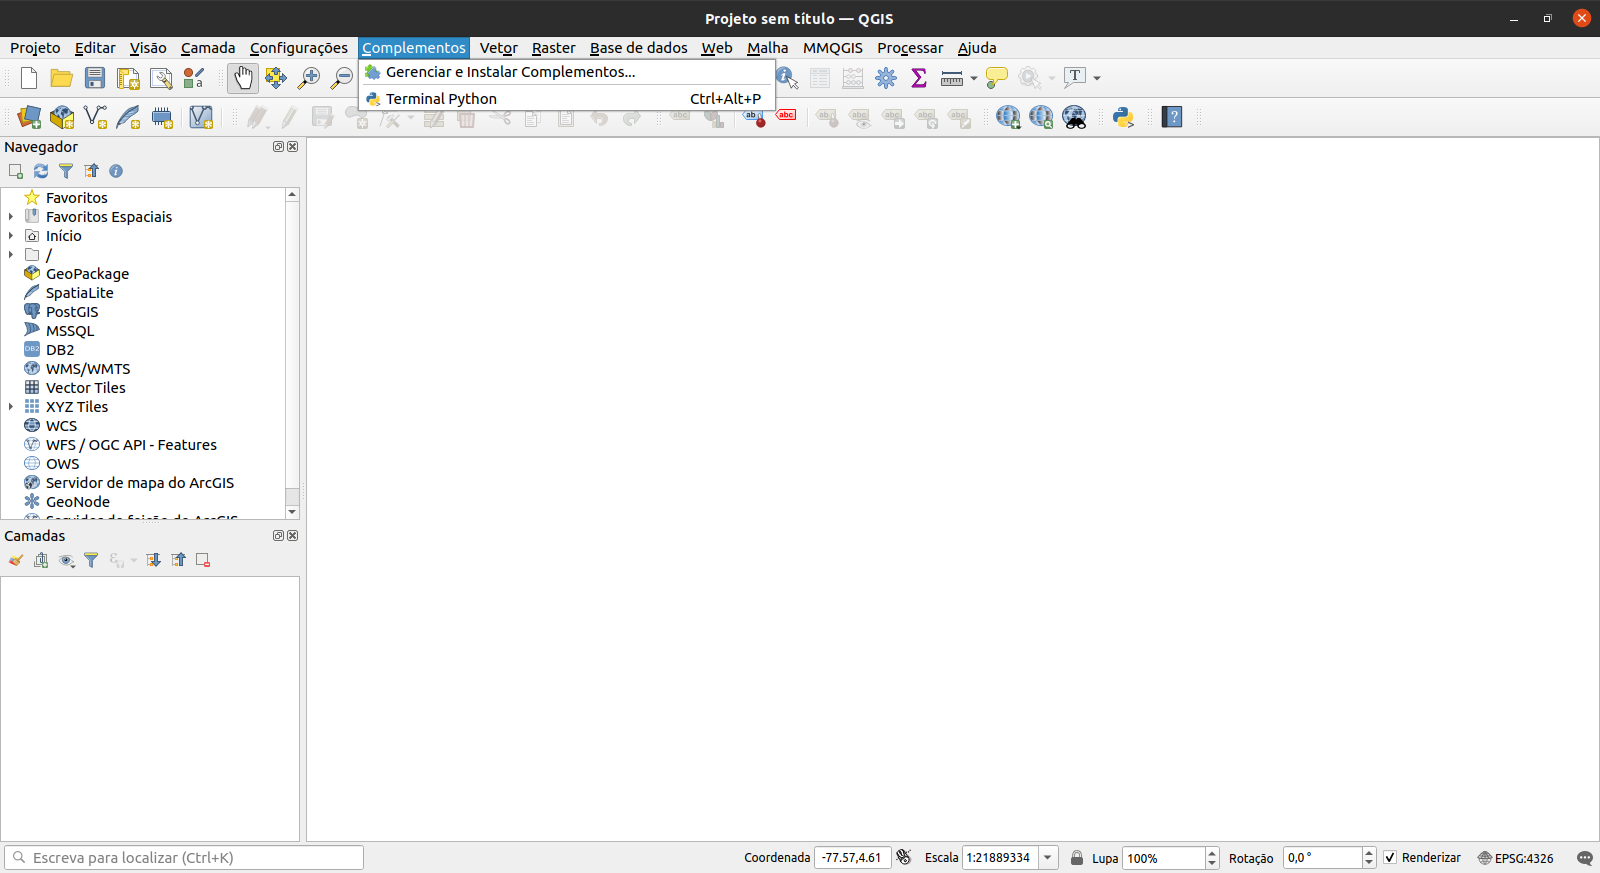
\includegraphics{media/modulo1/plugins-menu.png}
\caption{Menu Gerenciar e Instalar Complementos}
\end{figure}

Figura 1.5. Acessando a caixa de diálogo Gerenciar e instalar complementos

\textbf{Diálogo Gerenciar e Instalar Complementos}

A caixa de diálogo Gerenciar e instalar complementos se conecta ao repositório de complementos oficiais do QGIS (ou qualquer repositório que você indicar na guia Configurações) para buscar complementos disponíveis para sua versão do QGIS. Possui cinco (5) abas:

\begin{itemize}
\tightlist
\item
  \textbf{Aba Tudo} - mostra TODOS os complementos disponíveis para sua versão QGIS, incluindo aqueles que já estão instalados em sua máquina
\item
  \textbf{Aba Instalados} - mostra apenas os complementos instalados em sua máquina
\item
  \textbf{Aba não instalado} - mostra os complementos que não estão instalados em sua máquina
\item
  \textbf{Aba Instalar a partir do do ZIP} - permite que você instale complementos de um arquivo ZIP
\item
  \textbf{Aba Opções} - oferece opções sobre quando verificar se há atualizações de complementos, incluir ou não complementos experimentais e obsoletos ou adicionar / alterar o repositório para buscar complementos
\end{itemize}

Se o complemento que você está procurando está marcado como experimental ou obsoleto, você precisa marcar \textbf{Mostrar complementos experimentais} e \textbf{Mostrar complementos obsoletos} na guia Opções.

A \textbf{Barra de Pesquisa} permite que você pesquise complementos encontrados no(s) repositório(s) de complementos aos quais você está conectado.

\begin{figure}
\centering
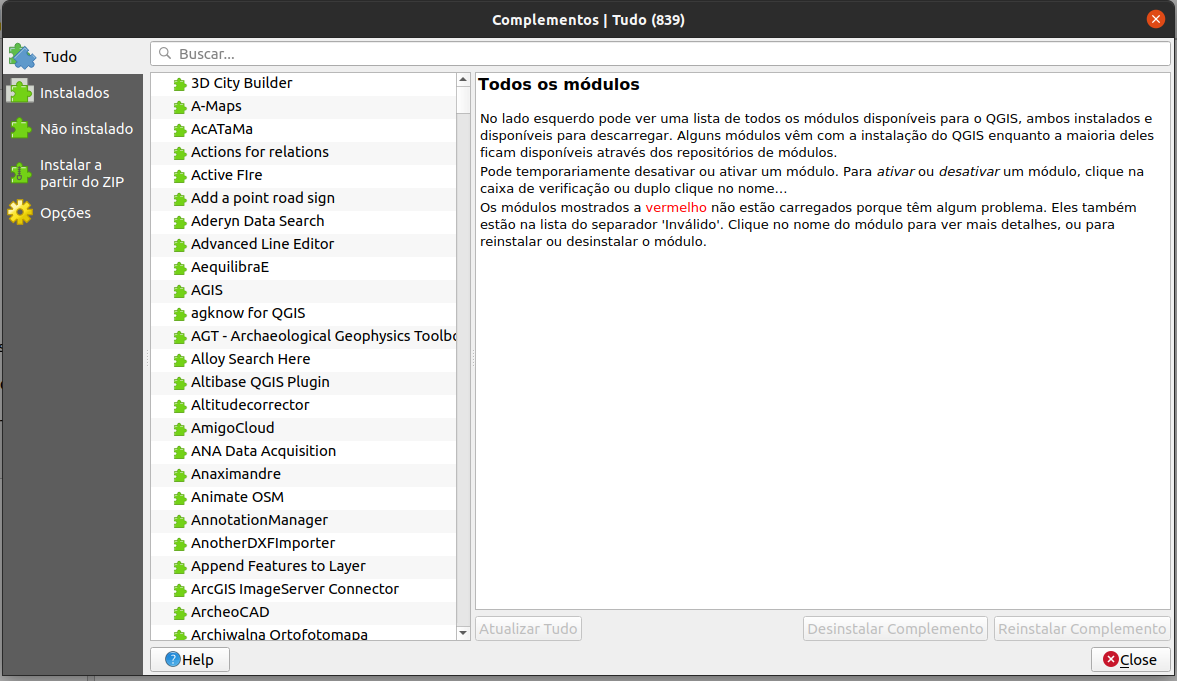
\includegraphics{media/modulo1/manage-and-install-plugins-dialog.png}
\caption{Caixa de diálogo Gerenciar e instalar complementos}
\end{figure}

Figura 1.6. A caixa de diálogo Gerenciar e instalar complementos

\hypertarget{tutorial-exercuxedcio-2-instalando-um-complemento-qgis}{%
\subsubsection{\texorpdfstring{\textbf{Tutorial / Exercício 2: Instalando um complemento QGIS}}{Tutorial / Exercício 2: Instalando um complemento QGIS}}\label{tutorial-exercuxedcio-2-instalando-um-complemento-qgis}}

\begin{enumerate}
\def\labelenumi{\arabic{enumi}.}
\tightlist
\item
  Abra a caixa de diálogo \textbf{Gerenciar e instalar complementos} em \textbf{Complementos ‣ Gerenciar e instalar complementos} na barra de menus. Isso abrirá a caixa de diálogo Gerenciar e instalar complementos.
\end{enumerate}

\begin{figure}
\centering
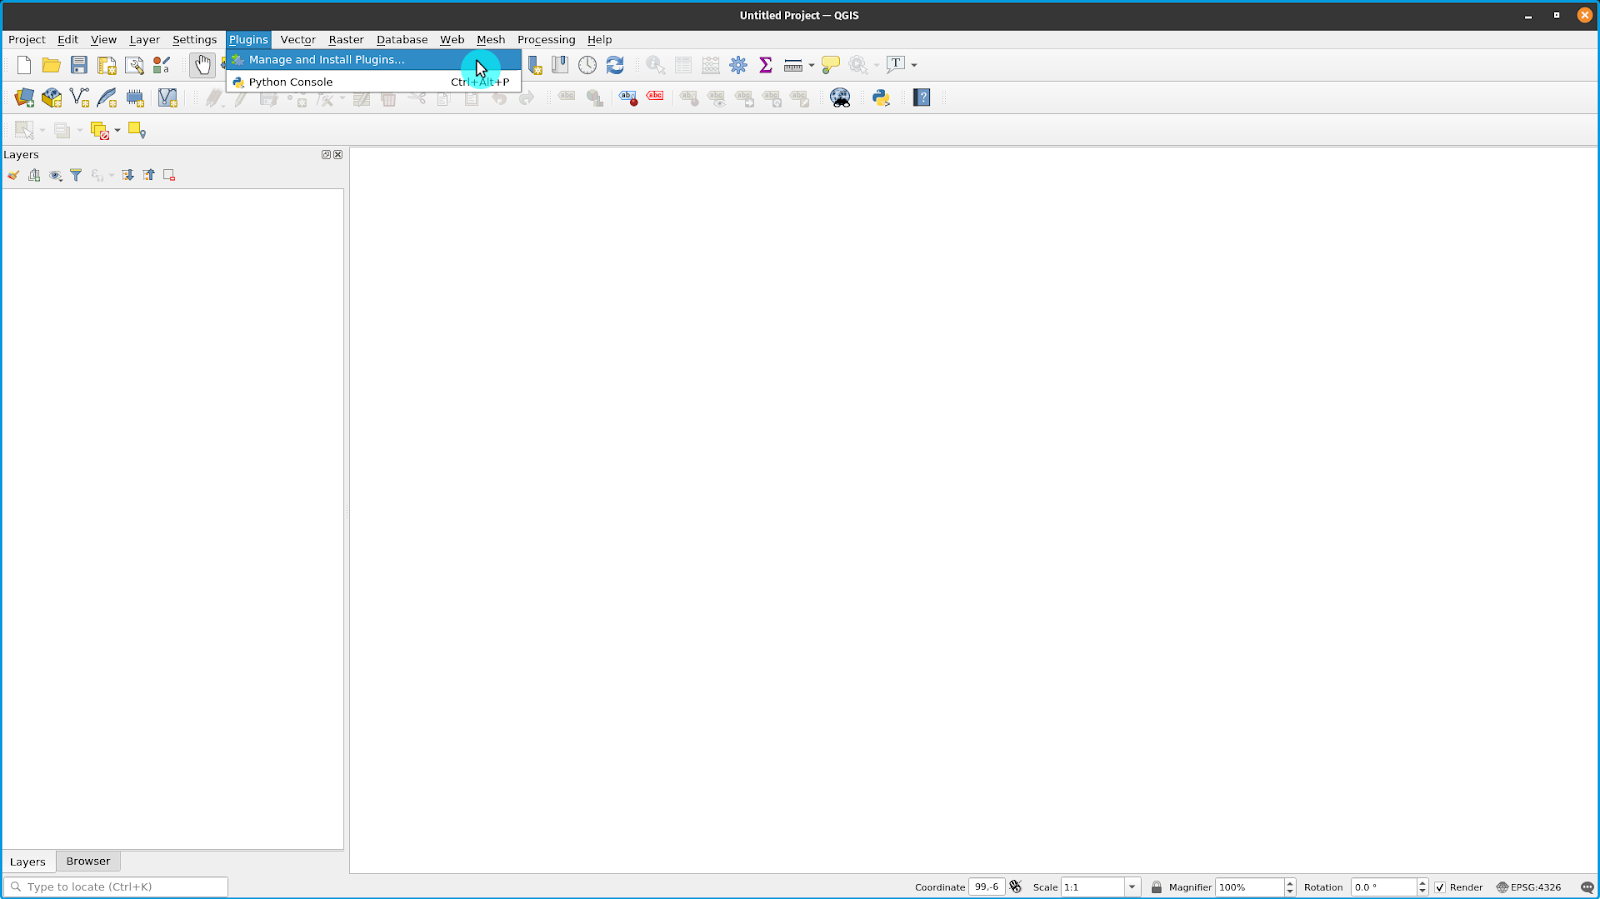
\includegraphics{media/modulo1/plugins-menu-2.png}
\caption{Abrir caixa de diálogo Gerenciar e instalar complementos}
\end{figure}

\begin{figure}
\centering
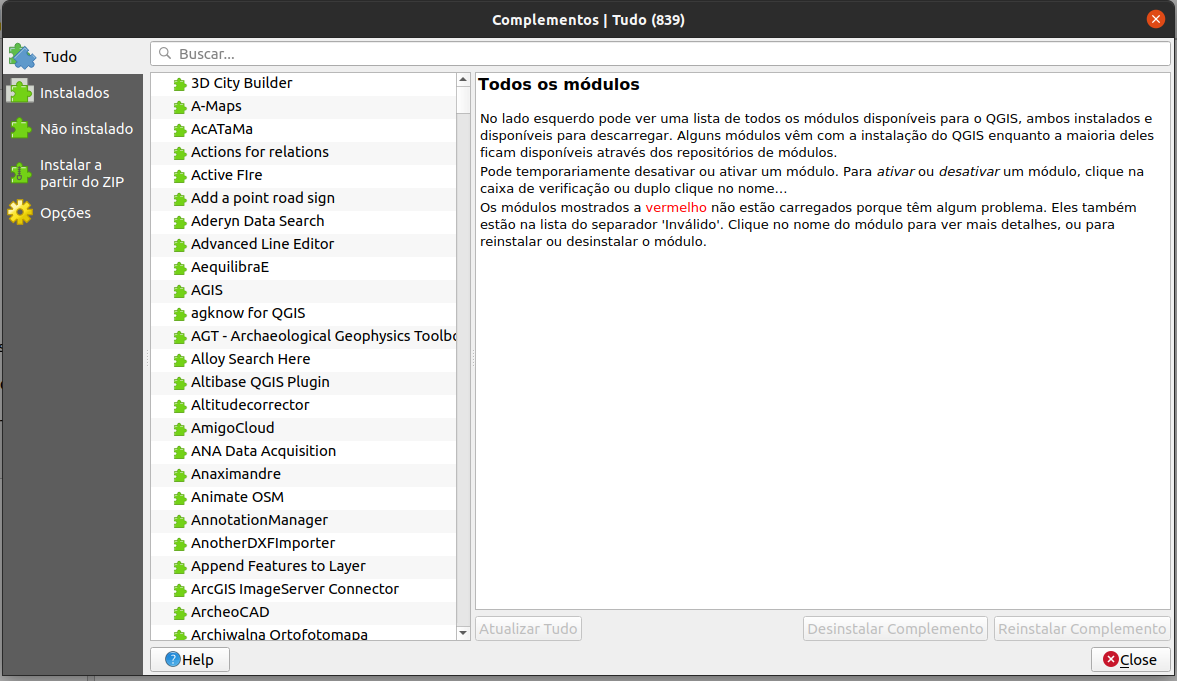
\includegraphics{media/modulo1/manage-and-install-plugins-dialog.png}
\caption{Caixa de diálogo Gerenciar e instalar complementos}
\end{figure}

\begin{enumerate}
\def\labelenumi{\arabic{enumi}.}
\setcounter{enumi}{1}
\tightlist
\item
  Instale os complementos a seguir procurando por eles na guia \textbf{Todos} e clicando em \textbf{Instalar complemento} no canto inferior direito da caixa de diálogo Gerenciar e instalar complementos.

  \begin{itemize}
  \tightlist
  \item
    Memory Layer Saver
  \end{itemize}
\end{enumerate}

\begin{figure}
\centering
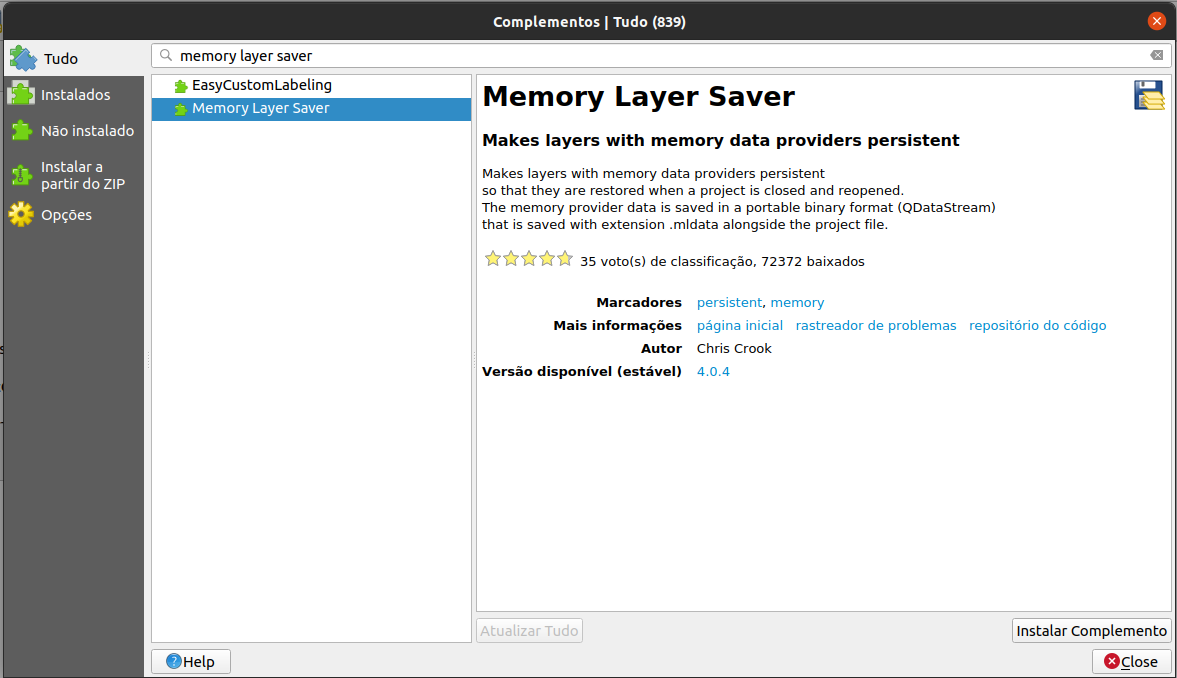
\includegraphics{media/modulo1/memory-layer-saver-plugin.png}
\caption{Instalar o plugin Memory Layer Saver}
\end{figure}

\begin{itemize}
\tightlist
\item
  QuickOSM
\end{itemize}

\begin{figure}
\centering
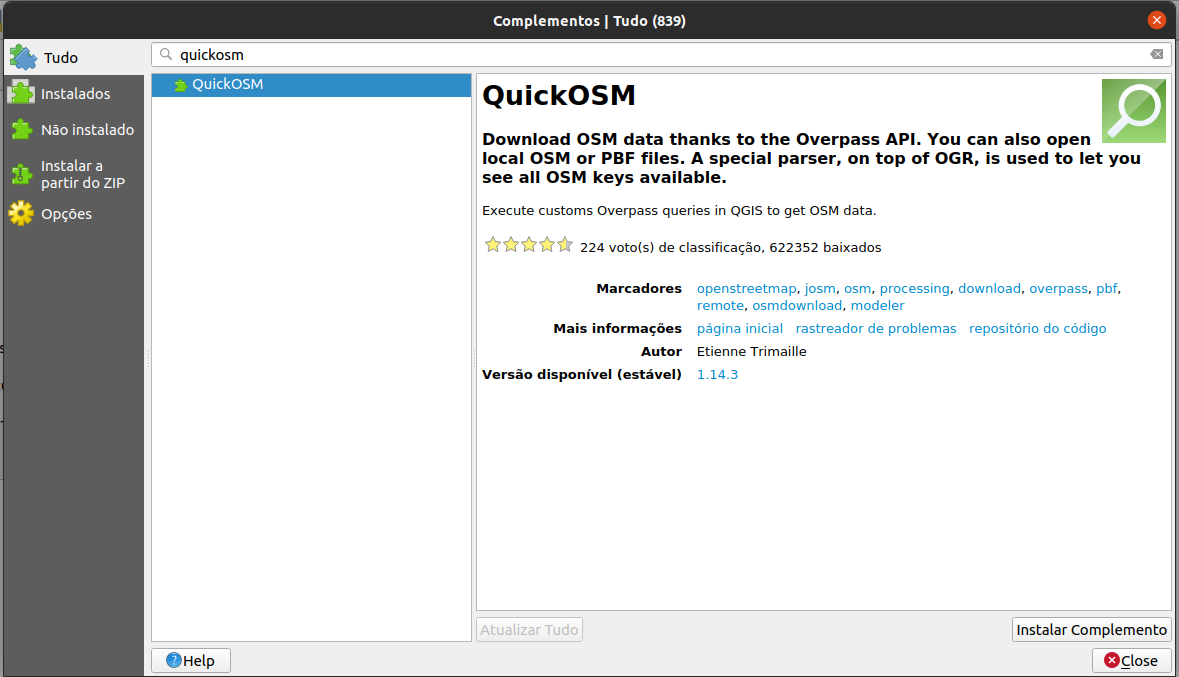
\includegraphics{media/modulo1/quickosm-plugin.png}
\caption{Instalar plugin QuickOSM}
\end{figure}

\begin{enumerate}
\def\labelenumi{\arabic{enumi}.}
\setcounter{enumi}{2}
\tightlist
\item
  Verifique se os complementos foram instalados com sucesso. O plugin Memory Layer Saver deve estar disponível em \textbf{Complementos ‣ Memory Layer Saver} na barra de menus, enquanto o plugin QuickOSM deve estar disponível em \textbf{Vetor ‣ QuickOSM} na barra de menus.
\end{enumerate}

\hypertarget{perguntas-do-questionuxe1rio-3}{%
\subsubsection{\texorpdfstring{\textbf{Perguntas do questionário}}{Perguntas do questionário}}\label{perguntas-do-questionuxe1rio-3}}

\begin{enumerate}
\def\labelenumi{\arabic{enumi}.}
\tightlist
\item
  Verdadeiro ou falso

  \begin{enumerate}
  \def\labelenumii{\arabic{enumii}.}
  \tightlist
  \item
    Você pode remover ou desinstalar os complementos do Core - \textbf{\emph{Falso}}
  \item
    Você pode adicionar complementos que não são encontrados no repositório oficial de complementos do QGIS - \textbf{\emph{Verdadeiro}}
  \end{enumerate}
\end{enumerate}

\hypertarget{tuxedtulo-da-fase-3-configurauxe7uxf5es-qgis}{%
\subsection{Título da Fase 3: Configurações QGIS}\label{tuxedtulo-da-fase-3-configurauxe7uxf5es-qgis}}

\textbf{Configurações do sistema e do projeto}

As configurações do QGIS permitem que você edite e gerencie coisas diferentes sobre o QGIS, como perfis de usuário, estilos, sistemas de referência de coordenadas, atalhos de teclado, a interface do usuário, cores padrão, etc. As configurações do sistema podem ser encontradas no menu \textbf{Configurações} e são as configurações padrão usadas pelo QGIS, a menos que sejam substituídas pelas configurações de um projeto. As configurações do projeto podem ser encontradas em \textbf{Projeto ‣ Propriedades} e referem-se às configurações ou propriedades do projeto atual. Esses valores substituem os padrões do sistema.

\begin{figure}
\centering
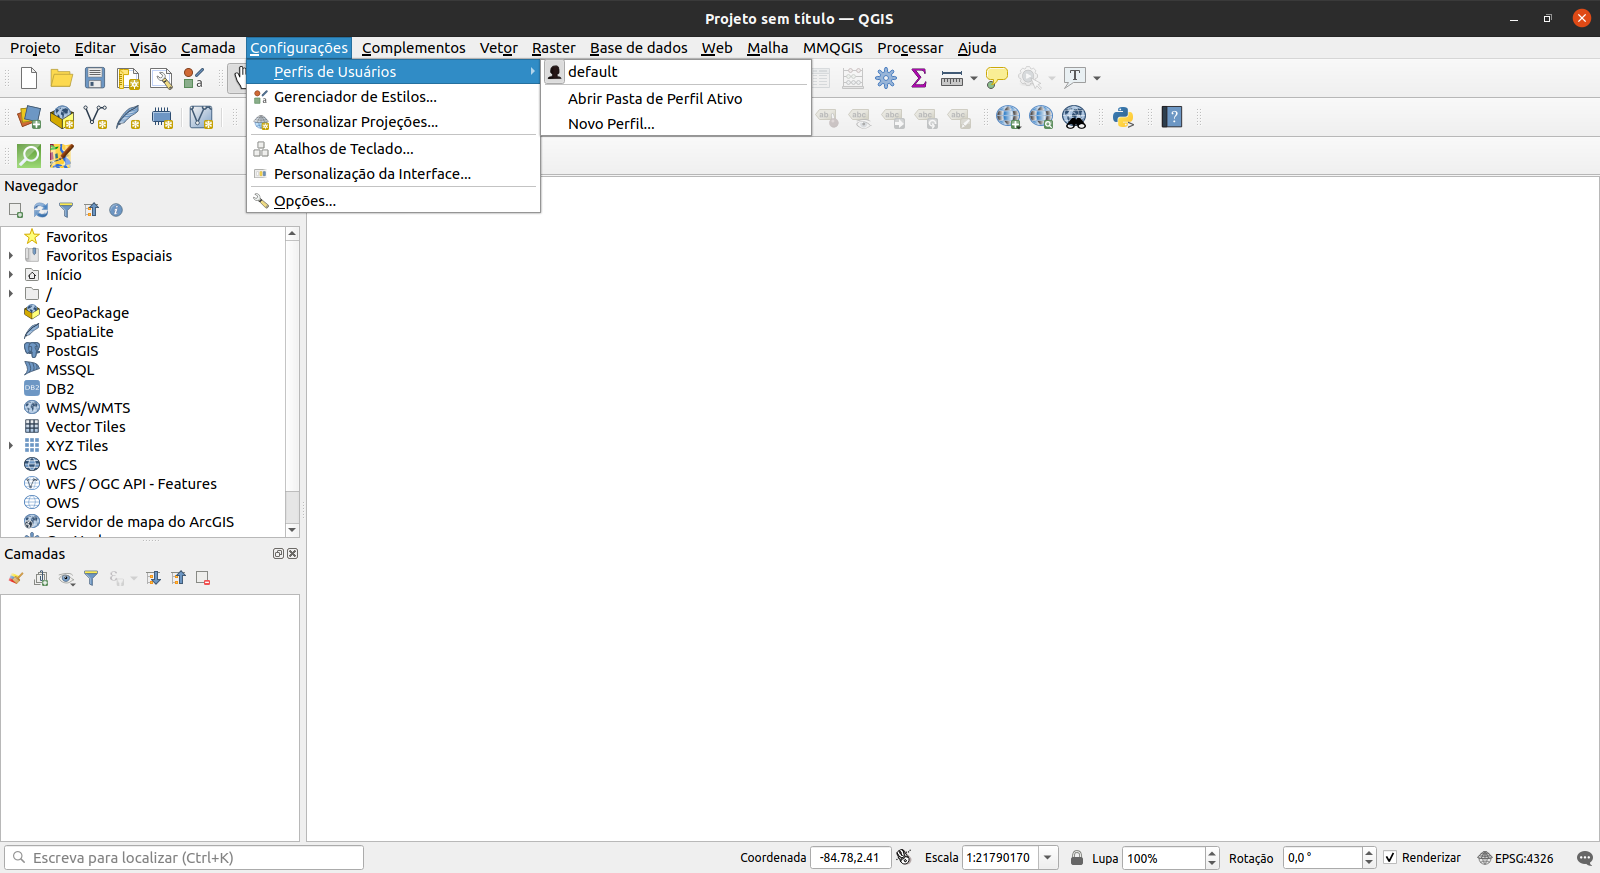
\includegraphics{media/modulo1/settings-1.png}
\caption{As Configurações do Sistema}
\end{figure}

Figura 1.7. As configurações do sistema

\begin{figure}
\centering
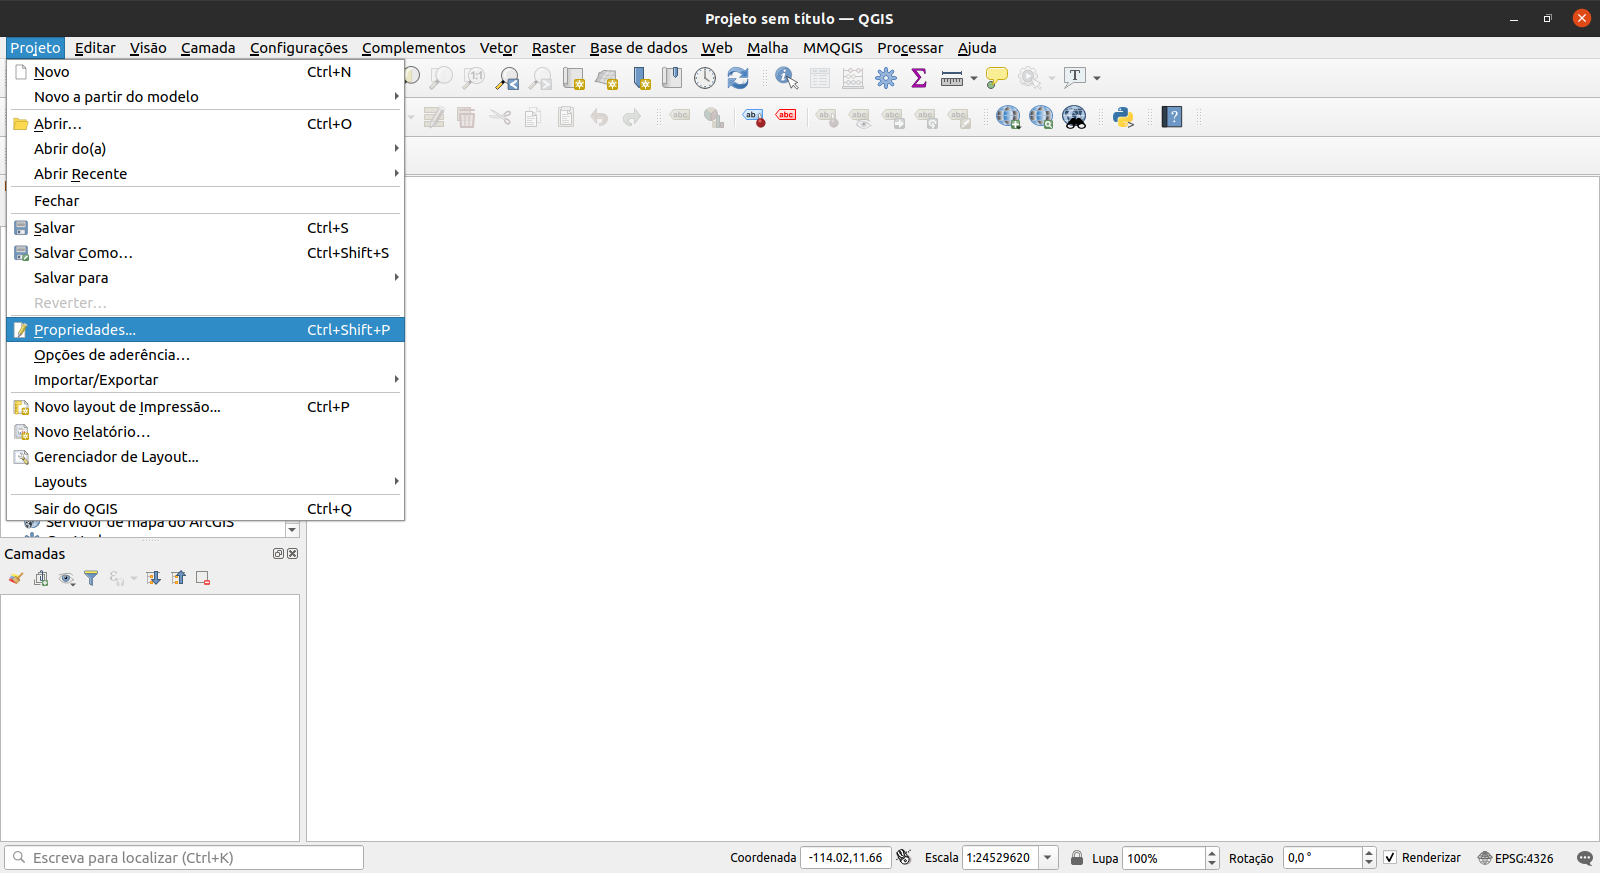
\includegraphics{media/modulo1/settings-2.png}
\caption{Configurações do projeto}
\end{figure}

Figura 1.8. Configurações do projeto

\textbf{Mudando o tema QGIS}

Você pode alterar a aparência do QGIS em \textbf{Configurações ‣ Opções ‣ Aba Geral}.

Você pode escolher entre três temas - padrão (default), Blend of Grey e Night Mapping. Você também pode alterar o tamanho dos ícones, a fonte usada pelo QGIS e outros padrões do sistema.

\begin{figure}
\centering
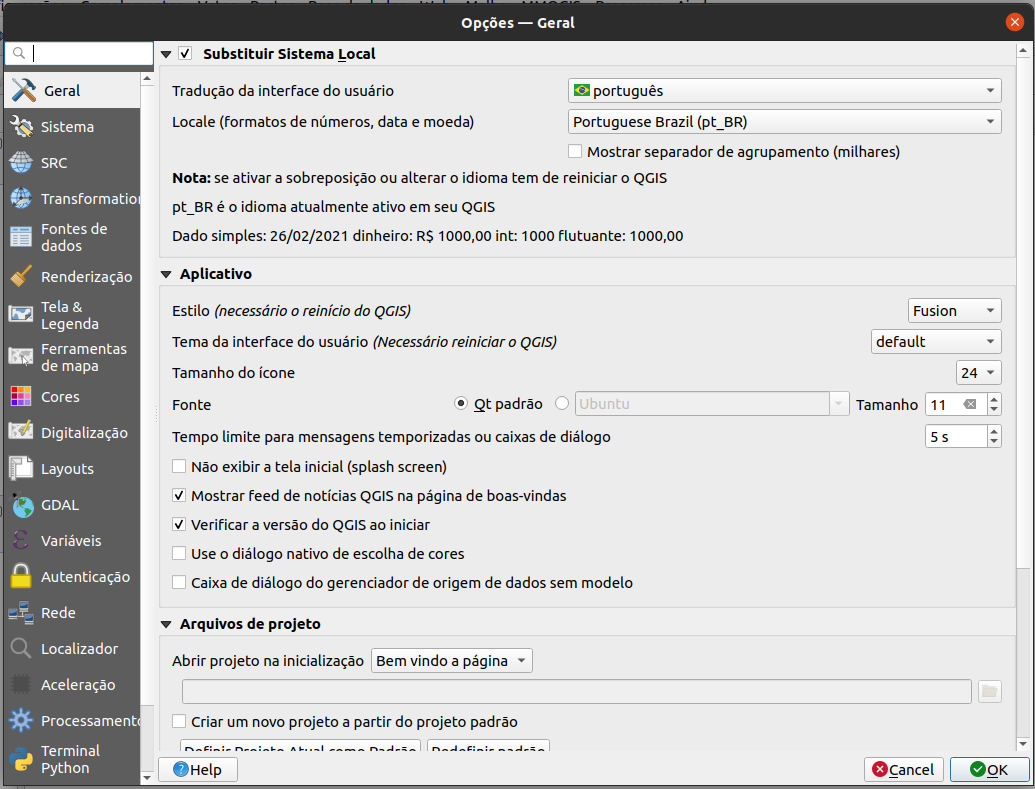
\includegraphics{media/modulo1/change-theme.png}
\caption{Configurações gerais do QGIS}
\end{figure}

Figura 1.9. Configurações gerais do QGIS

Para algumas configurações no QGIS, pode ser necessário reiniciar o aplicativo para que tenham efeito.

\textbf{Perfis de usuário}

QGIS 3.X introduziu o conceito de Perfis de Usuário QGIS.

Um perfil de usuário é uma coleção de configurações para complementos instalados, barras de ferramentas habilitadas, organização da interface do usuário e outras configurações. QGIS vem com um Perfil de Usuário padrão chamado default. Perfis de usuário permitem que o usuário crie configurações diferentes para análises específicas (por exemplo, um perfil de usuário específico para gestão de recursos hídricos, digitalização de dados, cartografia, etc.), projetos particulares ou mesmo clientes.

Perfis de usuário podem ser criados e acessados na barra de menus em: \textbf{Configurações ‣ Perfis de usuário}.

O perfil de usuário ativo é mostrado com {[}Perfil do usuário{]} na barra de título.

\begin{figure}
\centering
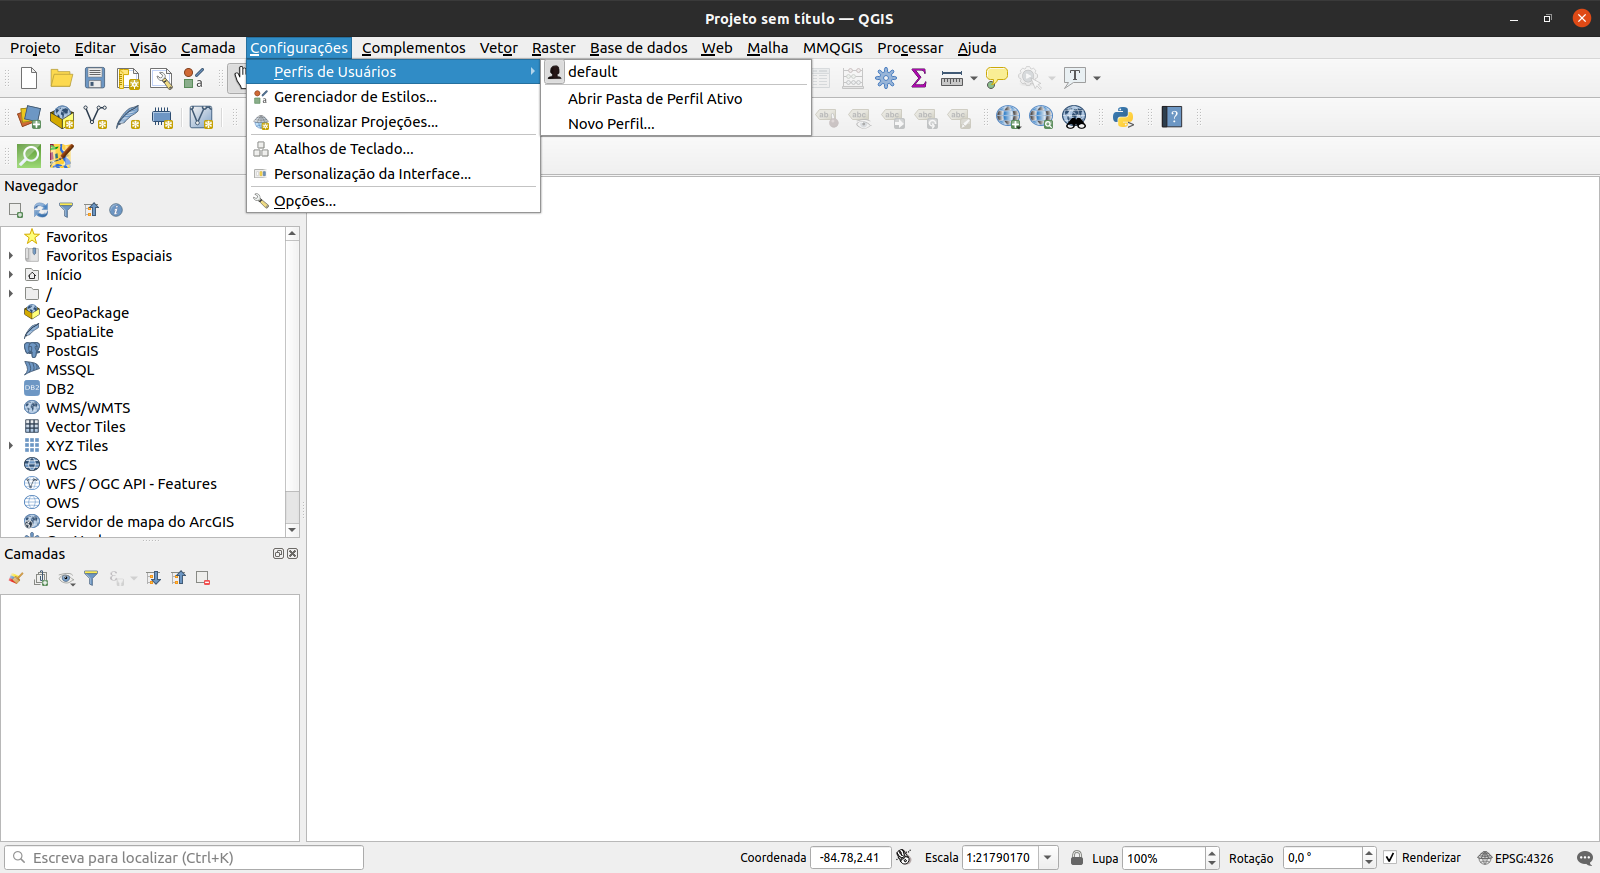
\includegraphics{media/modulo1/user-profiles-1.png}
\caption{Acessando perfis de usuário}
\end{figure}

Figura 1.10. Acessando perfis de usuário

Os perfis de usuário são salvos em um diretório em seu computador que pode ser acessado clicando em \textbf{Configurações ‣ Perfis de usuário ‣ Abrir pasta de perfil ativo}.

\hypertarget{tutorial-exercuxedcio-03-criando-um-perfil-de-usuuxe1rio}{%
\subsubsection{\texorpdfstring{\textbf{Tutorial / Exercício 03: Criando um Perfil de Usuário}}{Tutorial / Exercício 03: Criando um Perfil de Usuário}}\label{tutorial-exercuxedcio-03-criando-um-perfil-de-usuuxe1rio}}

\begin{enumerate}
\def\labelenumi{\arabic{enumi}.}
\tightlist
\item
  Vá para \textbf{Configurações ‣ Perfis de usuário ‣ Novo perfil \ldots{}}
\end{enumerate}

\begin{figure}
\centering
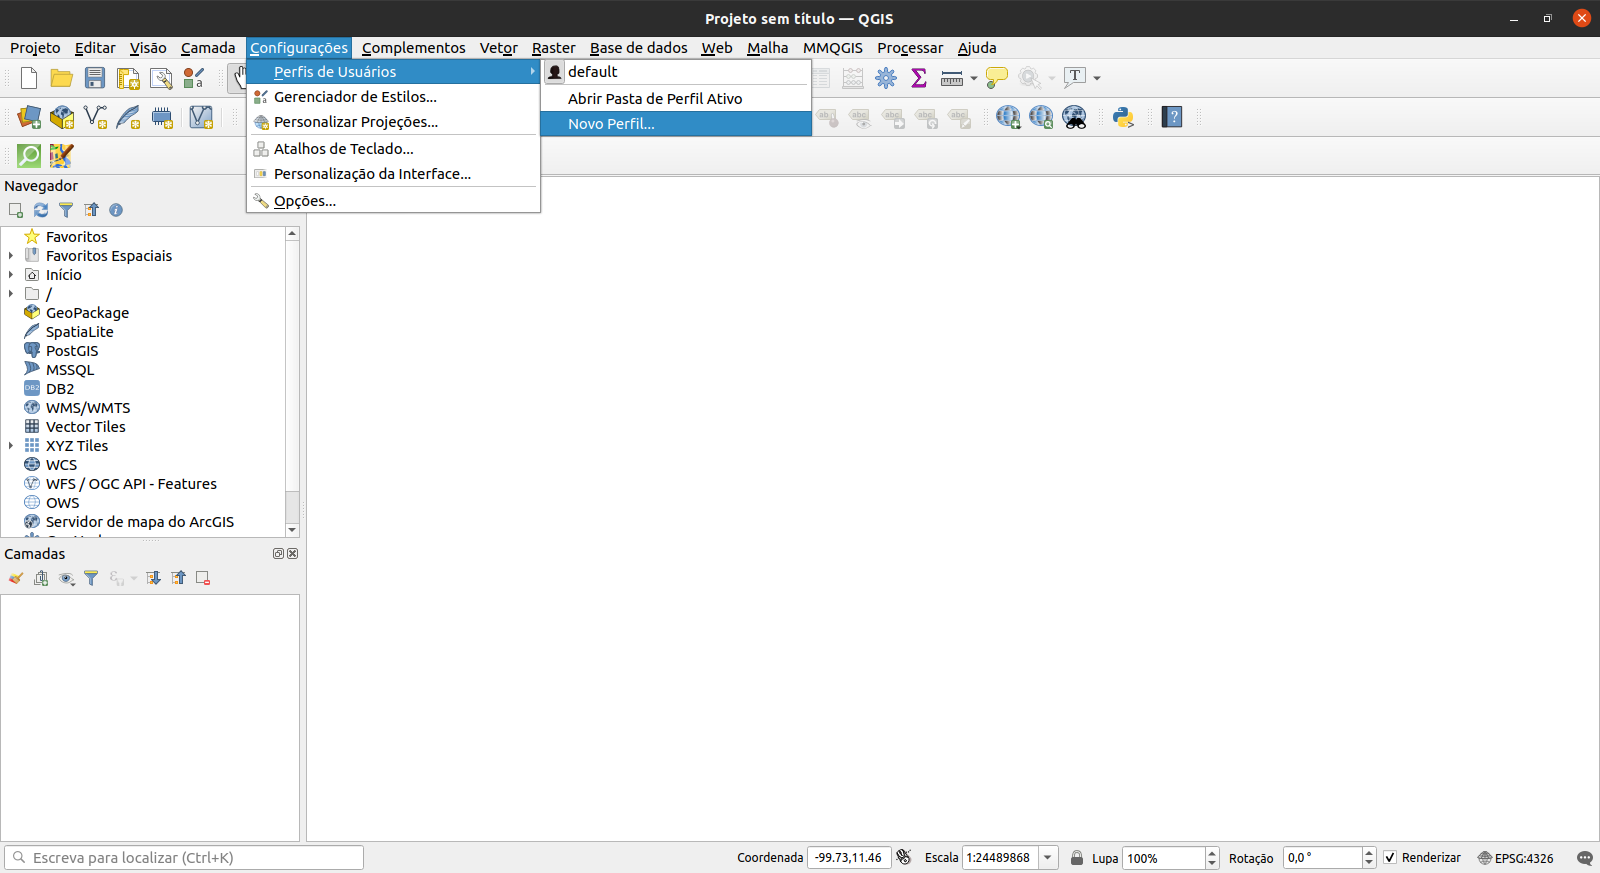
\includegraphics{media/modulo1/user-profiles-2.png}
\caption{alt\_text}
\end{figure}

\begin{enumerate}
\def\labelenumi{\arabic{enumi}.}
\setcounter{enumi}{1}
\tightlist
\item
  Dê um nome ao seu novo perfil de usuário.
\end{enumerate}

\begin{figure}
\centering
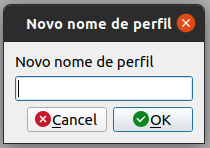
\includegraphics{media/modulo1/user-profiles-3.png}
\caption{alt\_text}
\end{figure}

\begin{enumerate}
\def\labelenumi{\arabic{enumi}.}
\setcounter{enumi}{2}
\item
  Uma nova janela QGIS deve abrir com seu novo perfil de usuário. Observe que o nome do seu perfil é mostrado na barra de título do QGIS.
\item
  Você percebe alguma diferença no novo perfil do usuário? Verifique a interface do usuário, os complementos e as configurações do perfil antigo e do novo perfil que você criou.
\end{enumerate}

\hypertarget{perguntas-do-questionuxe1rio-4}{%
\subsubsection{\texorpdfstring{\textbf{Perguntas do questionário}}{Perguntas do questionário}}\label{perguntas-do-questionuxe1rio-4}}

\begin{enumerate}
\def\labelenumi{\arabic{enumi}.}
\tightlist
\item
  Verdadeiro ou falso

  \begin{enumerate}
  \def\labelenumii{\arabic{enumii}.}
  \tightlist
  \item
    Você só pode ter um perfil de usuário no QGIS. - \textbf{\emph{Falso (você pode ter vários perfis de usuário)}}
  \item
    Você não pode substituir as configurações e propriedades do sistema. - \textbf{\emph{Falso}}
  \end{enumerate}
\end{enumerate}

\hypertarget{tuxedtulo-da-fase-4-adicional-formatos-de-arquivo-do-qgis}{%
\subsection{Título da Fase 4 (adicional): Formatos de arquivo do QGIS}\label{tuxedtulo-da-fase-4-adicional-formatos-de-arquivo-do-qgis}}

\hypertarget{arquivo-de-projeto-qgis-qgs-qgz}{%
\subsubsection{\texorpdfstring{\textbf{Arquivo de projeto QGIS (QGS / QGZ)}}{Arquivo de projeto QGIS (QGS / QGZ)}}\label{arquivo-de-projeto-qgis-qgs-qgz}}

Projetos QGIS estão para QGIS como arquivos .mxd são para ArcMap. Esses arquivos vêm como \textbf{QGS (\emph{.qgs)\textbf{ ou }QGZ (}.qgz)}. A principal diferença entre os dois é que o formato QGZ é um arquivo compactado (zip) contendo um arquivo QGS e um arquivo QGD. O formato QGS é um formato XML para armazenar projetos QGIS. O arquivo QGD é o banco de dados sqlite associado do projeto QGIS que contém dados auxiliares para o projeto. Se não houver dados auxiliares, o arquivo QGD ficará vazio.

Um arquivo de projeto QGIS contém tudo o que é necessário para armazenar um projeto QGIS, incluindo:

\begin{itemize}
\tightlist
\item
  título do projeto
\item
  CRS do projeto
\item
  a árvore de camadas
\item
  configurações de ajuste
\item
  relações
\item
  a extensão da tela do mapa
\item
  modelos de projeto
\item
  legend
\item
  docas mapview (2D e 3D)
\item
  as camadas com links para os conjuntos de dados subjacentes (fontes de dados) e outras propriedades da camada, incluindo extensão, CRS, junções, estilos, renderizador, modo de mesclagem, opacidade e muito mais
\item
  propriedades do projeto
\end{itemize}

Os arquivos do projeto QGIS podem ser salvos em um banco de dados GeoPackage ou PostGIS. Salvar o arquivo do projeto junto com o arquivo de estilo e as camadas correspondentes em um único GeoPackage facilita o compartilhamento de projetos QGIS.

\hypertarget{definiuxe7uxe3o-da-camada-qgis-qlr}{%
\subsubsection{\texorpdfstring{\textbf{Definição da camada QGIS (QLR)}}{Definição da camada QGIS (QLR)}}\label{definiuxe7uxe3o-da-camada-qgis-qlr}}

Um arquivo de definição de camada QGIS (\textbf{QLR}) é um arquivo XML que contém um ponteiro para a fonte de dados da camada, além das informações de estilo QGIS para a camada. Atualmente, um arquivo QLR corresponde a uma única camada apenas.

O caso de uso para este arquivo é simples: ter um único arquivo para abrir uma fonte de dados e trazer todas as informações de estilo relacionadas. Os arquivos QLR também permitem definir a fonte de dados subjacente em um arquivo fácil de abrir.

Um exemplo de uso de QLR é para abrir uma camada de um banco de dados PostGIS. Em vez de se conectar ao banco de dados, encontrar a camada e aplicar um filtro, você pode apenas abrir um arquivo .qlr que aponta para a camada PostGIS correta com seu estilo e filtro correspondentes.

\hypertarget{arquivo-de-estilo-qgis-qml}{%
\subsubsection{\texorpdfstring{\textbf{Arquivo de estilo QGIS (QML)}}{Arquivo de estilo QGIS (QML)}}\label{arquivo-de-estilo-qgis-qml}}

\textbf{QML} é um formato XML para armazenar estilos de camadas. Um arquivo QML (.qml) contém todas as informações que dizem ao QGIS como renderizar geometrias de feições que incluem definições de símbolos, tamanhos e rotações, rótulos, opacidade, modo de mesclagem e muito mais.

Um arquivo .qml deve ter o mesmo nome da fonte de dados a que ele corresponde. Quando ele for encontrado no mesmo diretório ou pasta da fonte de dados, carregar a fonte de dados também carregará automaticamente seu estilo, conforme definido no arquivo .qml.

Por exemplo, se você tiver um GeoJSON chamado \texttt{regioes.geojson} e um arquivo QML chamado \texttt{regioes.qml}, carregar as \texttt{regioes.geojson} no QGIS aplicará os estilos definidos em \texttt{regioes.qml} na camada carregada.

Ao usar GeoPackages (.gpkg), um arquivo .qml muitas vezes não é necessário, pois você pode salvar o estilo de uma camada diretamente no geopacote.

\hypertarget{se-vocuxea-quiser-ir-mais-longe-1}{%
\subsection{Se você quiser ir mais longe:}\label{se-vocuxea-quiser-ir-mais-longe-1}}

Você pode tentar criar seu próprio plugin QGIS. Se não houver um complemento que faça o que você deseja, você pode criar um você mesmo.

O \textbf{Plugin Builder} é um plugin que cria um modelo que pode servir como ponto de partida para o desenvolvimento do plugin QGIS para que você não precise criar um desde o início. Você pode instalá-lo na caixa de diálogo Gerenciar e instalar complementos.

Claro, você sempre pode criar um plugin do zero. Se você estiver interessado em criar seu próprio plugin, pode verificar a documentação oficial do QGIS (\url{https://documentation.qgis.org/}). Para complementos Python, é uma boa ideia verificar o PyQGIS Developer Cookbook (\href{https://docs.qgis.org/3.16/en/docs/pyqgis_developer_cookbook\%20/}{https://docs.qgis.org/3.16/en/docs/pyqgis\_developer\_cookbook/}).

Para obter mais informações, consulte: \href{https://bnhr.xyz/2018/10/08/qgis-plugins-3.0.\%20html}{https://bnhr.xyz/2018/10/08/qgis-plugins-3.0.html}

\hypertarget{para-praticar-suas-novas-habilidades-tente-1}{%
\subsection{Para praticar suas novas habilidades, tente \ldots{}}\label{para-praticar-suas-novas-habilidades-tente-1}}

\begin{itemize}
\tightlist
\item
  Altere o tema e a aparência da interface do usuário QGIS de acordo com sua preferência.
\item
  Instale outros complementos QGIS.
\item
  Altere outras configurações do QGIS.

  \begin{itemize}
  \tightlist
  \item
    Crie um sistema de referência de coordenadas personalizado
  \item
    Adicione uma tela inicial personalizada (\href{https://bnhr.xyz/2020/09/05/custom-splash\%20-screen-qgis.html}{https://bnhr.xyz/2020/09/05/custom-splash-screen-qgis.html})
  \end{itemize}
\end{itemize}

\hypertarget{dicas-1}{%
\subsection{Dicas}\label{dicas-1}}

N/D

\hypertarget{camadas-no-qgis}{%
\chapter{Camadas no QGIS}\label{camadas-no-qgis}}

\textbf{Autor}: Ben Hur

\hypertarget{introduuxe7uxe3o-pedaguxf3gica-2}{%
\section{Introdução Pedagógica}\label{introduuxe7uxe3o-pedaguxf3gica-2}}

Este módulo irá ensinar-lhe os conceitos básicos das camadas no QGIS e como carregá-las. No final deste módulo, os alunos devem estar familiarizados com:

\begin{itemize}
\tightlist
\item
  as diferentes fontes de dados e formatos de arquivo que podem ser carregados no QGIS
\item
  as diferentes maneiras que os dados podem ser carregados no QGIS
\item
  alguns formatos de arquivo de dados comuns
\end{itemize}

Eles também devem ser capazes de:

\begin{itemize}
\tightlist
\item
  carregar camadas (vetores e rasters) usando o painel do navegador e o gerenciador de fonte de dados
\item
  conectar o QGIS a serviços remotos
\item
  trabalhar com camadas temporárias e virtuais
\item
  instalar alguns plug-ins que carregarão outros conjuntos de dados no QGIS
\item
  mostrar propriedades da camada, como metadados informações
\item
  salvar e exportar camadas
\end{itemize}

\hypertarget{ferramentas-e-recursos-necessuxe1rios-2}{%
\section{Ferramentas e recursos necessários}\label{ferramentas-e-recursos-necessuxe1rios-2}}

As ferramentas e recursos necessários para este módulo são:

\begin{itemize}
\tightlist
\item
  computador
\item
  conexão à Internet
\item
  QGIS 3.16 instalado no computador (\href{https://qgis.org/en/site/forusers/download.html}{https://qgis.org/en/site/forusers /download.html})
\end{itemize}

\hypertarget{pruxe9-requisitos-2}{%
\section{Pré-requisitos}\label{pruxe9-requisitos-2}}

\begin{itemize}
\tightlist
\item
  conhecimento básico de operação de um computador
\item
  familiaridade com formatos de dados espaciais e a interface QGIS (conclusão dos Módulos 0 e 1)
\end{itemize}

\hypertarget{recursos-adicionais-2}{%
\section{Recursos adicionais}\label{recursos-adicionais-2}}

\begin{itemize}
\tightlist
\item
  QGIS User Guide - \url{https://docs.qgis.org/3.16/en/docs/user_manual/}
\item
  Manual de treinamento QGIS - \url{https://docs.qgis.org/3.16/en/docs/training_manual/index.html}
\item
  Basemaps no QGIS - \url{https://bnhr.xyz/2018/10/07/basemaps-in-qgis.html}
\item
  Conectando o QGIS ao Serviços remotos - {[}\url{https://bnhr.xyz/2018/10/12/connecting-qgis-to-remote-services.html}{]} (\url{https://bnhr.xyz/2018/10/12/connecting-qgis-to} -remote-services.html)
\item
  Spreadsheet Layers Plugin - \href{https://bnhr.xyz/2018/\%2027/07\%20/\%20plugin-fridays-spreadsheet-layers-plugin.html}{https://bnhr.xyz/2018/07/27/plugin-fridays-spreadsheet-layers-plugin.html}
\end{itemize}

\hypertarget{introduuxe7uxe3o-temuxe1tica-2}{%
\section{Introdução temática}\label{introduuxe7uxe3o-temuxe1tica-2}}

\begin{figure}
\centering
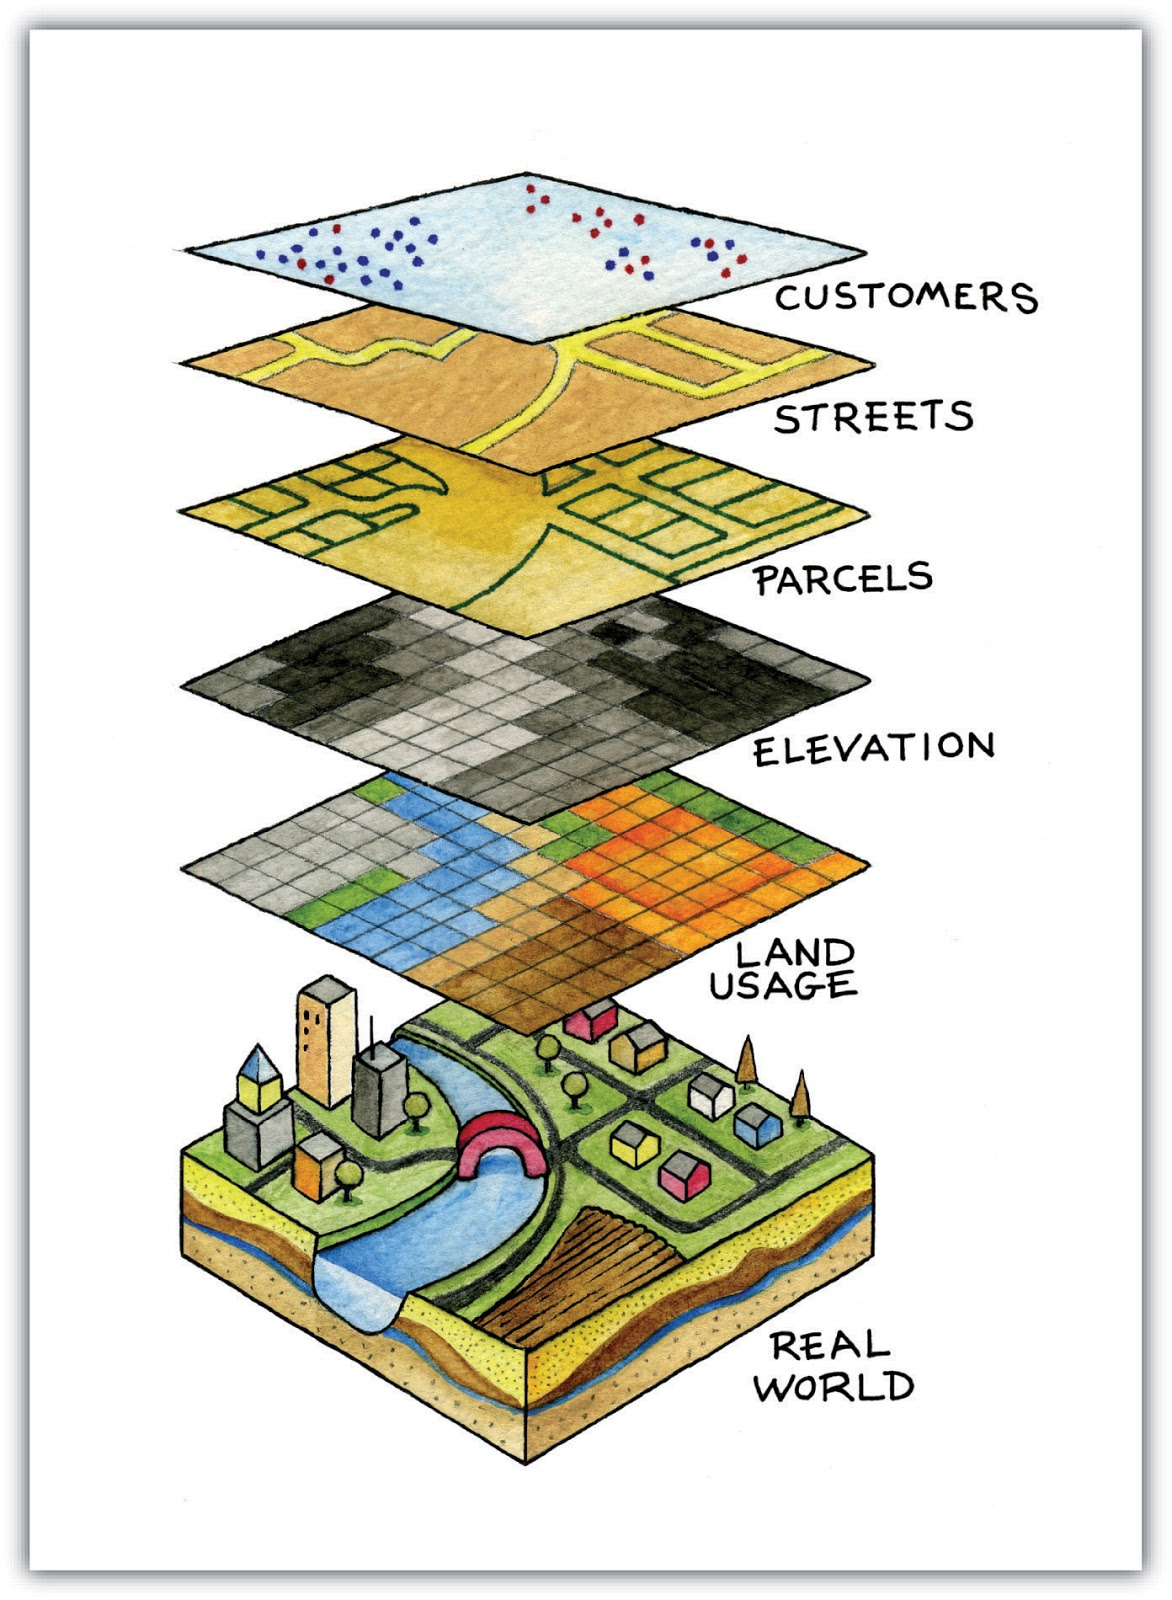
\includegraphics{media/modulo2/spatial-layers.jpg}
\caption{Análise de múltiplas camadas em GIS}
\end{figure}

Figura 2.1. Uma sobreposição de mapa contendo diferentes camadas e tipos de dados (\href{https://saylordotorg.\%20github.io/text_essentials-of-geographic-information-systems/s11-02-multiple-layer-analysis.html}{https://saylordotorg.github.io/text\_essentials-of-geographic-information-systems/s11-02-multiple-layer-analysis.html})

Aprendemos nos módulos anteriores que modelos de dados espaciais, como vetores e rasters, são modelos de objetos do mundo real e fenômenos e, embora seja perfeitamente normal ter uma única camada que modele uma única coisa (por exemplo, elevação, temperatura, localização de residências, zoneamento, etc.), na prática, se quisermos realizar análises úteis ou criar um modelo que reflita o mundo real melhor, então, precisaríamos usar vários dados e camadas juntos. Sobrepor vários mapas temáticos da mesma área, colocando-os uns sobre os outros, é uma das técnicas de análise geográfica mais antigas e comuns.

\hypertarget{detalhamento-dos-conceitos-1}{%
\section{Detalhamento dos conceitos}\label{detalhamento-dos-conceitos-1}}

A imagem acima nos dá um exemplo simples e concreto disso. Imagine que você é um consultor GIS encarregado de encontrar a melhor localização para uma nova escola. Para fazer isso, você precisaria reunir as informações relevantes que o ajudariam a decidir. Isso pode incluir informações sobre as ruas da cidade, lotes de terreno, localização e distribuição de possíveis estudantes, a topografia da área, uso do solo, etc.

Esses conjuntos de dados podem vir em diferentes tipos e formatos. Alguns podem ser arquivos vetoriais, enquanto outros podem ser raster. Alguns podem estar no mesmo sistema de referência de coordenadas, enquanto outros podem estar em sistemas de referência de coordenadas diferentes. Alguns podem ser arquivos locais encontrados em seu computador, enquanto outros só podem ser carregados pela Internet. Por causa das muitas possibilidades do tipo de dados que você precisaria para sua análise espacial, um bom GIS deve ser capaz de manipular e gerenciar uma variedade de fontes de dados.

\hypertarget{conteuxfado-principal-2}{%
\section{Conteúdo principal}\label{conteuxfado-principal-2}}

\hypertarget{tuxedtulo-da-fase-1-tipos-de-dados-formatos-de-arquivo-o-painel-do-navegador-e-o-painel-de-camadas}{%
\subsection{Título da fase 1: Tipos de dados, formatos de arquivo, o painel do navegador e o painel de camadas}\label{tuxedtulo-da-fase-1-tipos-de-dados-formatos-de-arquivo-o-painel-do-navegador-e-o-painel-de-camadas}}

\hypertarget{tipos-de-dados-e-formatos-de-arquivo-comuns}{%
\subsubsection{\texorpdfstring{\textbf{Tipos de dados e formatos de arquivo comuns}}{Tipos de dados e formatos de arquivo comuns}}\label{tipos-de-dados-e-formatos-de-arquivo-comuns}}

Além dos modelos de dados espaciais (rasters e vetores) discutidos no primeiro módulo, a familiaridade com formatos de arquivo geoespaciais e seus prós e contras também é importante para qualquer pessoa que faça análise espacial.

A maioria das pessoas que são novas em GIS geralmente são apresentadas aos dados espaciais por meio de shapefiles. A maioria das pessoas nunca supera esse formato e usa shapefiles para todos os tipos e formas de dados vetoriais. Isso é semelhante a como uma marca específica como a Coca Cola começa a ser usada como o termo geral para refrigerantes. Isso não é necessariamente errado, mas é lamentável, pois os shapefiles são apenas um dos muitos tipos de formato de dados vetoriais. Na verdade, há muitos outros formatos de vetor como geopackage, geojson, topojson e flatgeobuf. O formato do shapefile, embora onipresente, tem algumas limitações significativas, como:

\begin{itemize}
\tightlist
\item
  Não é apenas um arquivo único. Na verdade, um shapefile consiste em vários arquivos, 3 dos quais são obrigatórios: .shp, .shx, .dbf. Todos os outros arquivos são chamados de arquivos secundários (sidecar).
\item
  Tem um limite de tamanho de 2 GB para cada arquivo individual.
\item
  Os nomes dos campos são limitados a 10 caracteres.
\item
  Colunas de atributos são limitadas a 255 colunas.
\item
  Não há suporte para alguns tipos de dados, como tempo.
\item
  Não armazena explicitamente topologia.
\end{itemize}

Outros formatos de dados, como GeoPackage, GeoJSON, TopoJSON e flatgeobuf, corrigem essas limitações dos shapefiles. Na verdade, QGIS e GRASS GIS mudaram para GeoPackage como o formato de arquivo vetorial padrão ao importar ou exportar camadas e, embora GeoPackage também tenha algumas limitações, é um formato completamente aberto e permite que a comunidade ajude a moldar o futuro do formato.

Então, se não shapefiles, o que você deve usar?

Não há nada de errado em usar shapefiles, especialmente se for adequado ao seu caso de uso. Se você não precisa de um conjunto de dados que vai além de 2 GB; se não houver problema em ter um limite de 10 caracteres para os nomes dos campos; ou se você estiver trabalhando com um pequeno número de arquivos localmente, um shapefile é totalmente adequado.

No entanto, se você deseja empacotar seu projeto QGIS junto com todas as camadas (vetores, rasters), estilos e modelos; ou você deseja compartilhar vários tipos de camadas e dados espaciais em um único arquivo, vale a pena dar uma olhada em um GeoPackage. GeoPackages e GeoJSONs também são compatíveis com a web e podem ser usados diretamente por bibliotecas de mapeamento da web, como Mapbox e Leaflet.

Você pode ler mais no link abaixo: \href{https://bnhr.xyz/2018/12/12/i-choose\%20-geopackage.html}{https://bnhr.xyz/2018/12/12/i-choose-geopackage.html}

Enquanto isso, qualquer formato que pode ser representado como uma grade de pixels ou células pode ser lido pelo QGIS como dados raster. Isso inclui formatos de imagem como PNG (.png) e JPEG (.jpg). É importante notar que embora todos os formatos de arquivo de imagem possam ser lidos como rasters, nem todos são georreferenciados ou contêm informações geoespaciais que nos permitem localizá-los corretamente na Terra. Para instâncias como essa, podemos usar o que é conhecido como um arquivo mundial (ou world) (\url{https://en.wikipedia.org/wiki/World_file}). Um arquivo world é um arquivo de dados de texto simples separado, cujo nome é o mesmo do arquivo raster ao qual pertence e cuja extensão de arquivo tem a letra w adicionada ao final. Por exemplo, o arquivo world para \textbf{world.png} será nomeado \textbf{world.pngw} ou \textbf{world.pgw}.

Alguns formatos de arquivo de imagem contêm georreferenciamento e informações explícitas e não precisam de um arquivo word. Alguns exemplos são GeoTIFFs (.tif ou tiff) e formato de arquivo ERDAS Imagine (.img).

Para obter mais informações sobre formatos de arquivo, você também pode acessar: \href{https://saylordotorg.\%20github.io/text_essentials-of-geographic-information-systems/s09-03-file-formats.html}{https://saylordotorg.github.io/text\_essentials-of-geographic-information-systems/s09-03-file-formats.html} Os

Dados geoespaciais também podem vir no formato de bancos de dados geoespaciais. Eles podem ser bancos de dados de nível empresarial, como o Postgres, gratuito e de código aberto, com extensão PostGIS (\url{https://postgis.net/}) ou ArcSDE, proprietário da ESRI. Existem também bancos de dados geográficos de arquivos que podem armazenar diferentes tipos de dados (por exemplo, vetores e rasters) dentro deles. Alguns exemplos são o OGC GeoPackage, gratuito e aberto (.gpkg) (\url{https://www.geopackage.org/}) e o formato patenteado File Geodatabase da ESRI (.gdb).

\hypertarget{tipos-de-fontes-de-dados}{%
\subsubsection{\texorpdfstring{\textbf{Tipos de fontes de dados}}{Tipos de fontes de dados}}\label{tipos-de-fontes-de-dados}}

Um dos recursos mais poderosos do QGIS é sua capacidade de conectar, carregar e usar diferentes dados espaciais e não espaciais de uma variedade de fontes. O QGIS pode abrir:

\begin{itemize}
\tightlist
\item
  arquivos raster e vetoriais
\item
  bancos de dados locais
\item
  arquivos e bancos de dados na Internet por meio de seu identificador de recurso uniforme (URI) ou localizador de recurso uniforme (URL),
\item
  serviços da web (serviços da web OSGeo e serviços da web ArcGIS), tile services e portais de dados como GeoNode
\item
  e muitos mais\ldots{}
\end{itemize}

O QGIS também pode conectar e carregar dados de serviços como dados SRTM da NASA, imagens do planeta, SentinelHub, Google Earth Engine e OpenStreetMap através de plug-ins.

Isso torna o QGIS um componente integral para qualquer infraestrutura ou fluxo de trabalho de dados espaciais.

\hypertarget{carregando-camadas-no-qgis}{%
\subsubsection{\texorpdfstring{\textbf{Carregando camadas no QGIS}}{Carregando camadas no QGIS}}\label{carregando-camadas-no-qgis}}

Existem várias maneiras de carregar camadas no QGIS. Estes incluem:

\begin{enumerate}
\def\labelenumi{\arabic{enumi}.}
\tightlist
\item
  \textbf{Arraste e solte} a camada na Tela do Mapa QGIS ou no Painel de Camadas. Esta pode ser a maneira mais fácil de carregar uma camada no QGIS, mas não é a abordagem recomendada, pois há várias coisas que podem dar errado ao usar esta abordagem, como ao carregar dados tabulares não espaciais, por exemplo CSVs.
\item
  Usando o \textbf{Painel do navegador}.
\item
  Usando o \textbf{Gerenciador de fonte de dados}.
\item
  Usando a \textbf{barra de ferramentas do Gerenciador de fonte de dados} e a \textbf{barra de ferramentas Gerenciar camadas}.
\end{enumerate}

** NOTA: ** \emph{Ao carregar camadas, as cores padrão de suas camadas podem ser diferentes das cores padrão mostradas neste módulo.}

\hypertarget{o-painel-do-navegador}{%
\subsubsection{\texorpdfstring{\textbf{O painel do navegador}}{O painel do navegador}}\label{o-painel-do-navegador}}

O \textbf{Painel do navegador} exibe uma árvore de arquivos que mostra os arquivos e pastas do seu computador, bem como as conexões com bancos de dados e servidores web. Por padrão, ele é encaixado no lado esquerdo da interface do usuário QGIS junto com o Painel de Camadas.

O painel do navegador expõe muitas funcionalidades para conectar, carregar e mostrar informações sobre camadas. Você também pode criar conexões para diretórios favoritos e marcadores espaciais no painel do navegador.

Para saber mais sobre o painel do navegador, acesse: \href{https://docs.qgis.org/3.16/en\%20/docs/user_manual/introduction/browser.html}{https://docs.qgis.org/3.16/en/docs/user\_manual/introduction/browser.html}

\hypertarget{exercuxedcio-01.1-o-painel-do-navegador}{%
\subsubsection{\texorpdfstring{\textbf{Exercício 01.1: O painel do navegador}}{Exercício 01.1: O painel do navegador}}\label{exercuxedcio-01.1-o-painel-do-navegador}}

\begin{enumerate}
\def\labelenumi{\arabic{enumi}.}
\tightlist
\item
  Abra o QGIS.
\item
  Verifique o painel do navegador (Figura 2.2). Se você não conseguir encontrar o painel do navegador, pode torná-lo visível em \textbf{Exibir ‣ Painéis ‣ Painel do navegador} na barra de menus.
\end{enumerate}

\begin{figure}
\centering
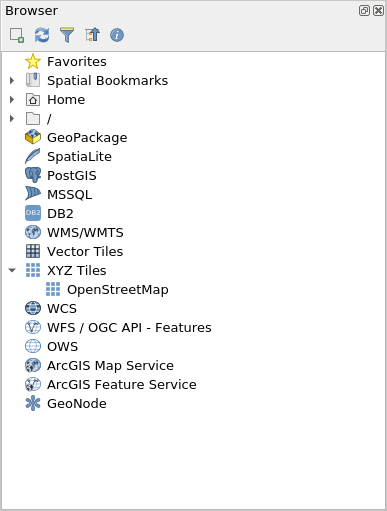
\includegraphics{media/modulo2/qgis-browser-1.png}
\caption{O painel do navegador QGIS}
\end{figure}

Figura 2.2. O painel do navegador

\begin{enumerate}
\def\labelenumi{\arabic{enumi}.}
\setcounter{enumi}{2}
\tightlist
\item
  Observe como os drives e pastas podem ser expandidas para mostrar as subpastas dentro delas.
\item
  Localize a pasta \textbf{Módulo 2 - Camadas no QGIS} (Figura 2.3) na árvore de arquivos (observe onde você salvou ou baixou o arquivo). Você deve ser capaz de ver os dados necessários para esta pasta de trabalho. No meu exemplo à direita, vinculei a pasta mencionada a um dos meus Favoritos para acessá-la facilmente no painel do navegador. Você pode adicionar um diretório favorito ao Painel do navegador clicando com o botão direito em Favoritos e adicionando o diretório.
\item
  Verifique os arquivos dentro da pasta (Figura 2.3). Existem vários deles. A partir da própria árvore de arquivos, já podemos ter uma ideia dos arquivos e camadas que podemos carregar no QGIS. Os ícones à esquerda dos nomes indicam se os dados são um vetor 
\includegraphics{media/modulo2/symbol-vector.png}, um raster 
\includegraphics{media/modulo2/symbol-raster.png}, um banco de dados 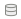
\includegraphics{media/modulo2/symbol-db.png} ou dados tabulares simples 
\includegraphics{media/modulo2/symbol-table.png}.
\end{enumerate}

\begin{figure}
\centering
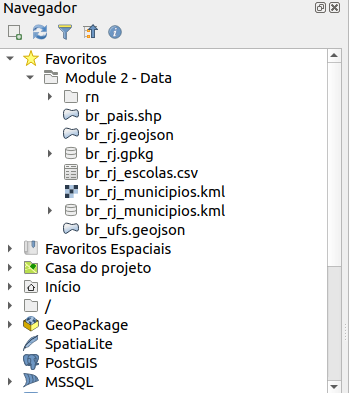
\includegraphics{media/modulo2/qgis-browser-2.png}
\caption{Arquivos do módulo 2 no painel do navegador}
\end{figure}

Figura 2.3. Os arquivos do módulo no painel do navegador

\begin{enumerate}
\def\labelenumi{\arabic{enumi}.}
\setcounter{enumi}{5}
\item
  Existem 5 arquivos na pasta de dados:

  \begin{enumerate}
  \def\labelenumii{\arabic{enumii}.}
  \tightlist
  \item
    um GeoPackage (br\_rj.gpkg) que contém um arquivo vetorial (br\_rj\_hospitais) e raster (br\_rj\_srtm\_dem);
  \item
    um GeoJSON (br\_ufs.geojson);
  \item
    um arquivo kml (br\_rj\_municipios.kml);
  \item
    um arquivo de forma (br\_pais.shp); e
  \item
    um arquivo de valores separados por vírgula (CSV) (br\_rj\_escolas.csv).
  \end{enumerate}
\item
  Clique com o botão direito em br\_pais.shp e clique em Propriedades da camada (Figura 2.4). Isso abre a janela de propriedades da camada (Figura 2.5). Observe as informações fornecidas na janela. Qual é a geometria da camada? Qual CRS é usado? Quantos recursos existem na camada?
\end{enumerate}

\begin{figure}
\centering
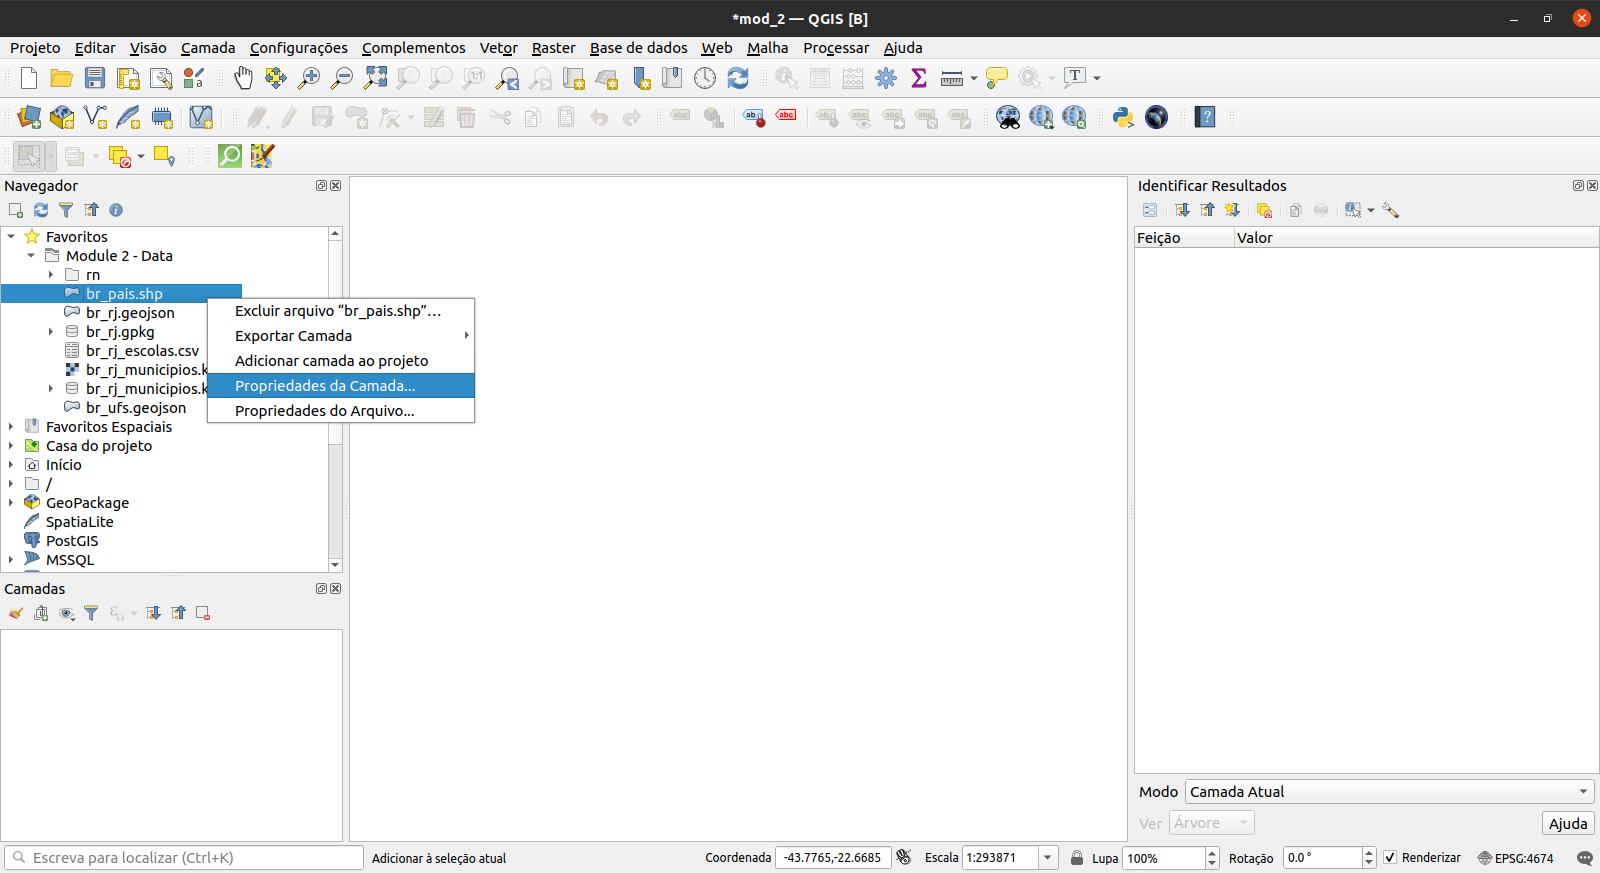
\includegraphics{media/modulo2/qgis-browser-3.png}
\caption{Verificando as propriedades da camada}
\end{figure}

Figura 2.4 Verificando as propriedades da camada

\begin{figure}
\centering
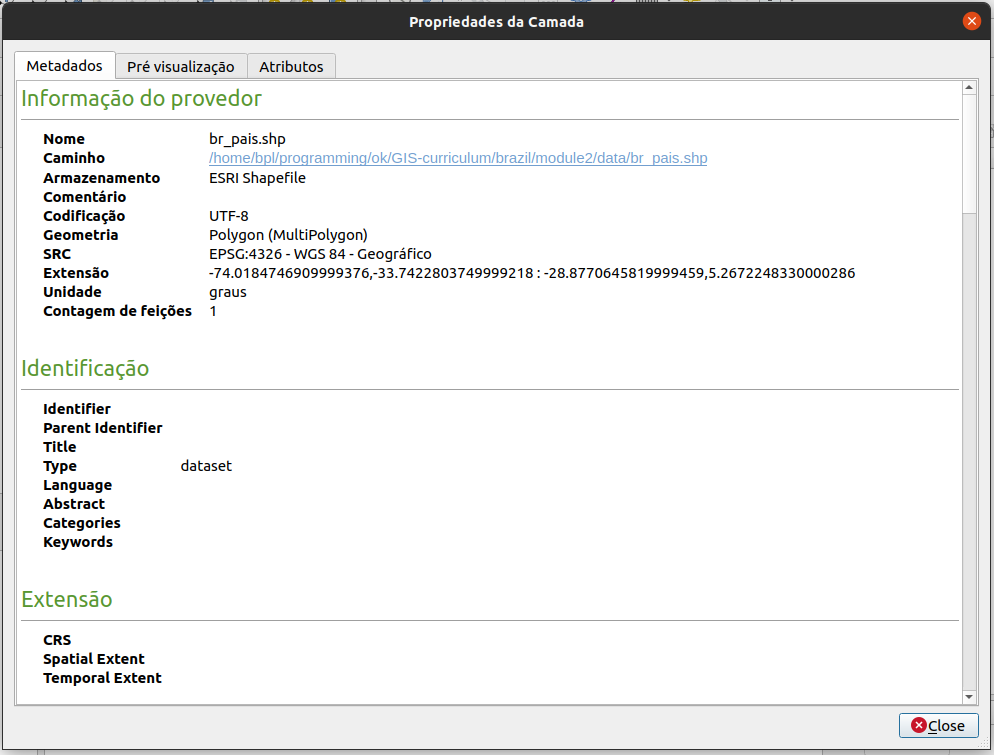
\includegraphics{media/modulo2/qgis-browser-layer-properties.png}
\caption{Propriedades da camada no painel do navegador}
\end{figure}

Figura 2.5. Propriedades da camada no painel do navegador

\begin{enumerate}
\def\labelenumi{\arabic{enumi}.}
\setcounter{enumi}{7}
\item
  Além de fornecer metadados nas camadas, você também pode visualizar a geometria e os atributos da camada na janela de propriedades da camada.
\item
  Você pode carregar uma camada do painel do navegador:

  \begin{enumerate}
  \def\labelenumii{\arabic{enumii}.}
  \tightlist
  \item
    \textbf{clicando duas vezes na camada}
  \item
    \textbf{clicando com o botão direito na camada ‣ Adicionar camada ao projeto}
  \item
    \textbf{arrastando a camada para a área do mapa}
  \end{enumerate}
\item
  Tente carregar as camadas \textbf{br\_pais}, \textbf{br\_ufs} e \textbf{br\_rj\_municipios} usando qualquer um dos métodos acima.
\end{enumerate}

\begin{figure}
\centering
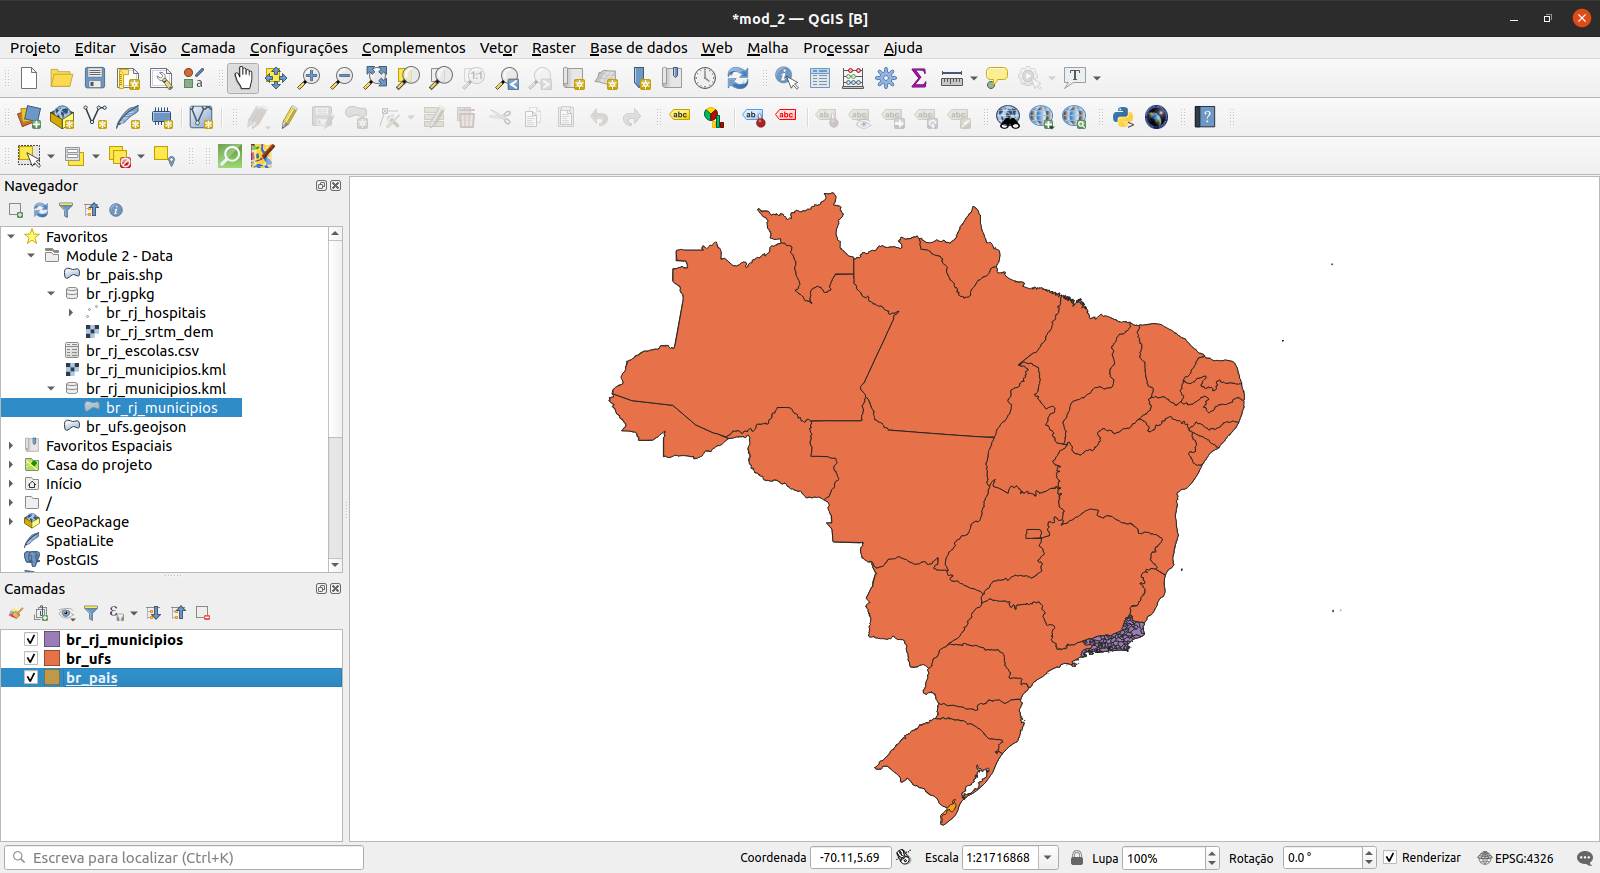
\includegraphics{media/modulo2/vector-layers-loaded-1.png}
\caption{As camadas vetoriais carregadas no QGIS}
\end{figure}

Figura 2.6. As camadas vetoriais carregadas no QGIS

\hypertarget{o-painel-de-camadas}{%
\subsubsection{\texorpdfstring{\textbf{O painel de camadas}}{O painel de camadas}}\label{o-painel-de-camadas}}

O painel de camadas lista todas as camadas atuais no projeto. Ele ajuda a gerenciar sua visibilidade e ordem e pode ser usado para mostrar as propriedades da camada. O painel de camadas pode ser ativado em \textbf{Exibir ‣ Painéis ‣ Painel de camadas} ou usando o atalho \textbf{CTRL + 1}. Ele também é chamado de legenda do mapa. Se você carregou todos os vetores do exercício anterior, seu painel de camadas deve aparecer como abaixo:

\begin{figure}
\centering
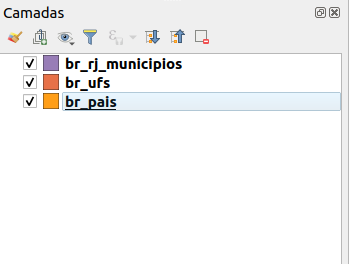
\includegraphics{media/modulo2/layers-panel-1.png}
\caption{Painel de camadas}
\end{figure}

Figura 2.7. O painel de camadas

A visibilidade de uma camada pode ser controlada marcando ou desmarcando a caixa à esquerda do nome da camada. Ao arrastar as camadas para cima ou para baixo no painel Camadas, sua ordem pode ser alterada. Semelhante ao software de manipulação de imagem como GIMP ou Photoshop, as camadas listadas perto do topo são desenhadas sobre as camadas listadas abaixo. Portanto, se duas camadas mostrarem a mesma área, a camada mais alta no painel camadas será desenhada no topo da camada inferior e pode ocultar a camada inferior na tela do mapa. É importante notar esse ponto porque pode haver casos em que pensamos que uma camada não aparece no QGIS quando na realidade está sendo coberta ou escondida por uma camada em cima dela.

\textbf{NOTA:} A ordem Z das camadas no Painel de camadas pode ser substituída pelo \textbf{Painel de ordem das camadas}.

O painel de camadas também permite ao usuário renomear e remover camadas, filtrar a visibilidade da camada, criar e gerenciar grupos de camadas e visualizações de mapas.

A tabela de atributos de uma camada vetorial também pode ser aberta no painel Camadas \textbf{clicando com o botão direito do mouse na camada ‣ Abrir tabela de atributos}.

Para saber mais sobre o painel de camadas, acesse: \href{https://docs.qgis.org\%20/3.16/en/docs/user_manual/introduction/general_tools.html\#layers-panel}{https://docs.qgis.org/3.16/en/docs/user\_manual/introduction/general\_tools.html\#layers-panel}

\hypertarget{propriedades-da-camada}{%
\subsubsection{\texorpdfstring{\textbf{Propriedades da camada}}{Propriedades da camada}}\label{propriedades-da-camada}}

Clicar com o botão direito em uma camada no painel Camadas e selecionar Propriedades da camada abrirá a caixa de diálogo Propriedades da camada.

\begin{figure}
\centering
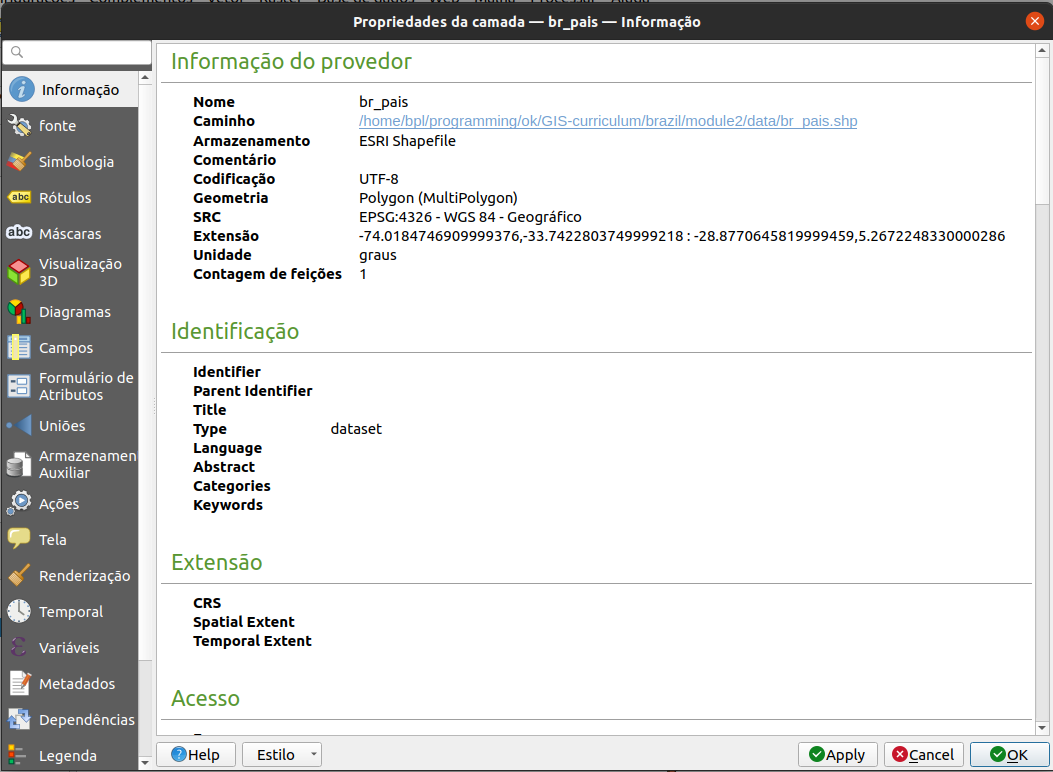
\includegraphics{media/modulo2/layer-properties.png}
\caption{A caixa de diálogo Propriedades da camada}
\end{figure}

Figura 2.8. A caixa de diálogo Propriedades da camada

Existem várias guias na caixa de diálogo Propriedades da camada que permitem ao usuário ver informações e até mesmo editar / modificar propriedades relacionadas à camada.

A guia Informações mostra uma representação somente leitura de informações resumidas e metadados da camada atual, incluindo:

\begin{itemize}
\tightlist
\item
  o provedor de dados
\item
  metadados
\item
  geometria ou informações de campo
\end{itemize}

A guia Fonte mostra as configurações gerais para uma camada vetorial.

Abas como Simbologia, Rótulos, Máscaras e Visualização 3D permitem que o usuário modifique a simbologia e o estilo da camada.

Outras guias permitem que os usuários realizem junções com a Camada (Junção), obtenham informações sobre os campos de atributos (Campos), adicionem Formulários personalizados para adicionar novos dados (Formulários de Atributo) e muito mais.

Outra guia que vale a pena mencionar é a guia Metadados, que fornece ao usuário a capacidade de criar e editar um relatório de metadados na camada. Isso inclui informações sobre:

\begin{itemize}
\tightlist
\item
  Identificação de dados: atribuição básica do conjunto de dados (dado pai, identificador, título, resumo, idioma \ldots);
\item
  Categorias às quais os dados pertencem, como categorias ISO e personalizadas;
\item
  Palavras-chave para recuperar os dados e conceitos associados seguindo um vocabulário padrão;
\item
  Acesso ao conjunto de dados (licenças, direitos, taxas e restrições);
\item
  Extensão do conjunto de dados, seja espacial (CRS, extensão do mapa, altitudes) ou temporal;
\item
  Contato do(s) proprietário(s) do conjunto de dados;
\item
  Links para recursos auxiliares e informações relacionadas; e
\item
  História do conjunto de dados.
\end{itemize}

Um resumo das informações preenchidas é fornecido na guia Validação e ajuda a identificar possíveis problemas relacionados ao formulário de metadados. Atualmente, os metadados são salvos no arquivo de projeto, mas também podem ser salvos em um arquivo .qmd separado ao lado das camadas baseadas em arquivo ou em um banco de dados .sqlite local para camadas remotas.

Para saber mais sobre as propriedades da camada vetorial, acesse: \href{https://docs.qgis.org/3.16/en\%20/docs/user_manual/working_with_vector/vector_properties.html}{https://docs.qgis.org/3.16/en/docs/user\_manual/working\_with\_vector/vector\_properties.html}

Para saber mais sobre as propriedades da camada raster, vá para: \href{https:\%20//docs.qgis.org/3.16/en/docs/user_manual/working_with_raster/raster_properties.html}{https://docs.qgis.org/3.16/en/docs/user\_manual/working\_with\_raster/raster\_properties.html}

\hypertarget{metadados-geoespaciais}{%
\subsubsection{\texorpdfstring{\textbf{Metadados geoespaciais}}{Metadados geoespaciais}}\label{metadados-geoespaciais}}

Metadados são simplesmente dados sobre os dados. Eles responde, o ``quem, o que, quando, onde e como'' dos dados e vem em todas as formas e tamanhos. Para fins de GIS, geralmente estamos preocupados com metadados geoespaciais. Os metadados geoespaciais são descritos pelo US Federal Geographic Data Committee (FGDC) como:

\emph{``um arquivo de informações, geralmente apresentado como um documento XML, que captura as características básicas de um recurso de dados ou informações. Representa quem, o quê, quando, onde, por que e como do recurso. Metadados geoespaciais comumente documentam dados digitais geográficos, como arquivos de Sistema de Informação Geográfica (GIS), bancos de dados geoespaciais e imagens da Terra, mas também podem ser usados para documentar recursos geoespaciais, incluindo catálogos de dados, aplicativos de mapeamento, modelos de dados e sites relacionados. Os registros de metadados incluem os principais elementos do catálogo da biblioteca, como Título, Resumo e Dados de Publicação; elementos geográficos, como extensão geográfica e informações de projeção; e elementos de banco de dados, como Definições de Rótulo de Atributo e Valores de Domínio de Atributo.''}

A importância dos metadados é que eles não apenas promovem a transparência, mas também facilitam o compartilhamento de dados e informações. É por isso que é importante sempre adicionar metadados aos nossos conjuntos de dados. Ao adicionar metadados, é igualmente importante seguir padrões - regras e práticas amplamente promovidas, aceitas e seguidas - para que os metadados que criamos sejam interoperáveis. Um desses padrões é a ISO 19115: 2014 ``Informação Geográfica - Metadados'' da ISO / TC 211 ({[}\url{https://www.iso.org/obp/ui/\#iso:std:iso:19115:-1:ed-1:v1:en}{]} (\url{https://www.iso.org/obp/ui/\#iso:std:iso:19115:-1:ed-1:v1:en}))

\hypertarget{exercuxedcio-01.2-adicionando-metadados}{%
\subsubsection{\texorpdfstring{\textbf{Exercício 01.2: Adicionando metadados}}{Exercício 01.2: Adicionando metadados}}\label{exercuxedcio-01.2-adicionando-metadados}}

\begin{enumerate}
\def\labelenumi{\arabic{enumi}.}
\tightlist
\item
  Abra as Propriedades da camada da camada br\_pais.
\item
  Verifique as informações mostradas na guia Informações e observe as informações mostradas. Está completo? Podemos adicionar mais informações?
\end{enumerate}

\begin{figure}
\centering
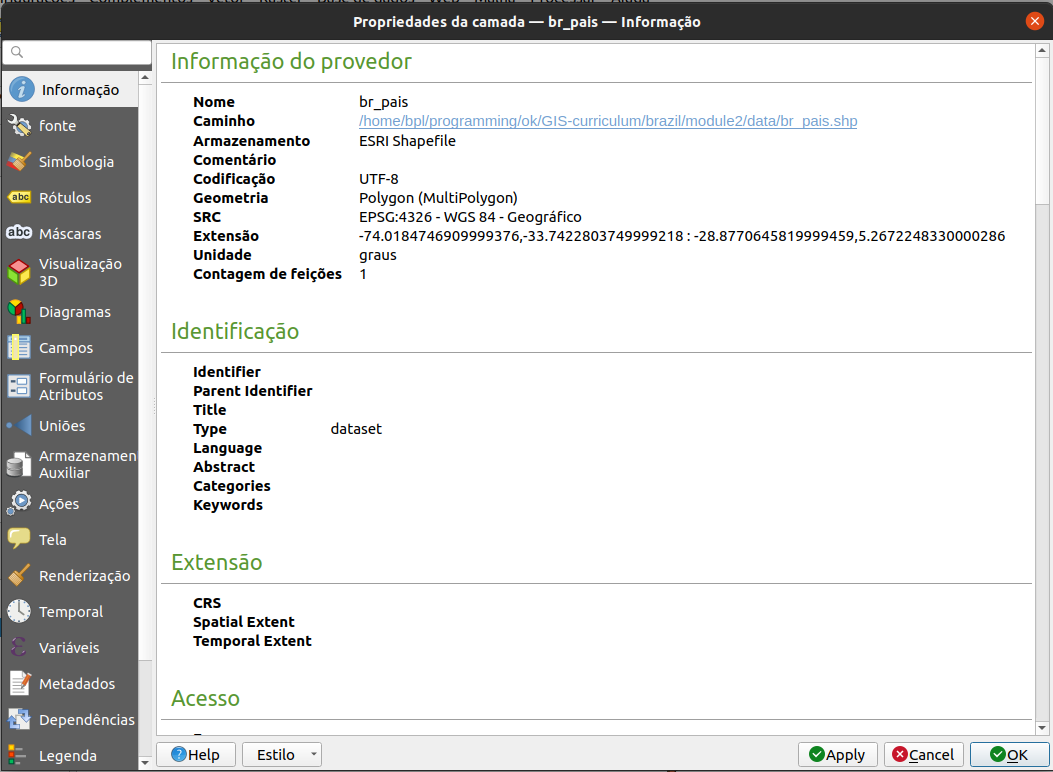
\includegraphics{media/modulo2/metadata-1.png}
\caption{Propriedades de informações da camada br\_pais}
\end{figure}

Figura 2.9. Propriedades de informações da camada br\_pais

\begin{enumerate}
\def\labelenumi{\arabic{enumi}.}
\setcounter{enumi}{2}
\tightlist
\item
  Vá para a guia Metadados e tente adicionar mais informações sobre a camada, como extensão, categoria de dados, licença, etc. Clique em OK quando terminar.
\end{enumerate}

\begin{figure}
\centering
\includegraphics{media/modulo2/metadata-2.png}
\caption{Editando alguns metadados}
\end{figure}

Figura 2.10. Editando alguns metadados

\begin{enumerate}
\def\labelenumi{\arabic{enumi}.}
\setcounter{enumi}{3}
\tightlist
\item
  Vá para a guia Informações novamente e veja se algo mudou.
\end{enumerate}

\begin{figure}
\centering
\includegraphics{media/modulo2/metadata-3.png}
\caption{A guia Informações após a edição de alguns metadados}
\end{figure}

Figura 2.11. A guia Informações depois de editar alguns metadados

\hypertarget{perguntas-do-questionuxe1rio-5}{%
\subsubsection{Perguntas do questionário}\label{perguntas-do-questionuxe1rio-5}}

\begin{enumerate}
\def\labelenumi{\arabic{enumi}.}
\item
  Verdadeiro ou falso:

  \begin{enumerate}
  \def\labelenumii{\arabic{enumii}.}
  \tightlist
  \item
    Todos os arquivos vetoriais são shapefiles. - *** Falso (um shapefile é um formato de arquivo de um arquivo vetorial. Outros formatos de arquivo de dados vetoriais incluem geopackage, geojson e flatgeobuf) ***
  \item
    Quando renderizado no mapa, uma camada que é superior no painel de camadas sempre cobrirá ou aparecerá no topo de uma camada que está abaixo no painel de camadas. - *** Falso (quando ativado, a ordem no painel de ordem de camadas substituirá a ordem no painel de camadas) ***
  \item
    Você pode verificar as informações de metadados sobre uma camada no painel Camadas e no painel do navegador. - *** Verdadeiro ***
  \end{enumerate}
\end{enumerate}

\hypertarget{tuxedtulo-da-fase-2-o-gerenciador-de-fonte-de-dados-e-conexuxe3o-com-serviuxe7os-remotos}{%
\subsection{Título da fase 2: O gerenciador de fonte de dados e conexão com serviços remotos}\label{tuxedtulo-da-fase-2-o-gerenciador-de-fonte-de-dados-e-conexuxe3o-com-serviuxe7os-remotos}}

\hypertarget{o-gerenciador-de-fonte-de-dados}{%
\subsubsection{\texorpdfstring{\textbf{O Gerenciador de fonte de dados}}{O Gerenciador de fonte de dados}}\label{o-gerenciador-de-fonte-de-dados}}

Se você não quiser usar o painel do navegador para carregar camadas, você sempre pode usar o \textbf{Gerenciador de fonte de dados}.

O \textbf{Gerenciador de fonte de dados} foi introduzido com o lançamento do QGIS 3. É um local único para adicionar e carregar camadas de diferentes fontes de dados no QGIS. Antes de sua introdução, havia janelas separadas para carregar diferentes fontes de dados (ou seja, uma para rasters, outra para vetores, etc.). Ele pode ser acessado via \textbf{Camadas ‣ Gerenciador de fonte de dados} ou \textbf{CTRL + L}.

\begin{figure}
\centering
\includegraphics{media/modulo2/data-source-manager-1.png}
\caption{Gerenciador de fonte de dados}
\end{figure}

Figura 2.12. O Gerenciador de fonte de dados

\hypertarget{exercuxedcio-02.1-o-gerenciador-de-fonte-de-dados}{%
\subsubsection{\texorpdfstring{\textbf{Exercício 02.1: O Gerenciador de fonte de dados}}{Exercício 02.1: O Gerenciador de fonte de dados}}\label{exercuxedcio-02.1-o-gerenciador-de-fonte-de-dados}}

\begin{enumerate}
\def\labelenumi{\arabic{enumi}.}
\item
  Abra o \textbf{Gerenciador de fonte de dados}. Ele contém guias no lado direito que pertencem ao tipo de fonte de dados que você deseja carregar ou conectar. Semelhante ao navegador, você pode carregar e conectar vários tipos de dados do Gerenciador de fonte de dados.
\item
  \textbf{Carregando vetores}

  \begin{enumerate}
  \def\labelenumii{\arabic{enumii}.}
  \item
    Para carregar vetores, vá para a guia Vetor. Podem ser carregados arquivos, arquivos dentro de um diretório, um banco de dados e até mesmo arquivos remotos por meio de um protocolo como HTTP, nuvem, etc.
  \item
    Vamos carregar o arquivo vetorial (br\_rj\_hospitais) encontrado dentro do geopackage br\_rj. Esta camada é uma camada de pontos das localizações dos hospitais na cidade do Rio de Janeiro.

    \begin{enumerate}
    \def\labelenumiii{\arabic{enumiii}.}
    \tightlist
    \item
      Tipo de fonte: Arquivo
    \item
      Fonte: Selecione o geopackage br\_rj usando o botão \includegraphics{media/modulo2/data-source-manager-search.png}
    \item
      Clique em Adicionar
    \item
      Se houver mais de 1 arquivo vetorial dentro do geopackage, o QGIS pedirá que você selecione quais carregar.
    \end{enumerate}
  \end{enumerate}
\end{enumerate}

\begin{figure}
\centering
\includegraphics{media/modulo2/data-source-manager-vector.png}
\caption{Carregando um vetor dentro de um GeoPackage}
\end{figure}

Figura 2.13. Carregando um vetor dentro de um GeoPackage

\begin{enumerate}
\def\labelenumi{\arabic{enumi}.}
\setcounter{enumi}{2}
\item
  \textbf{Carregando Rasters}

  \begin{enumerate}
  \def\labelenumii{\arabic{enumii}.}
  \item
    Para carregar um raster, vá para a aba Raster. Arquivos e arquivos remotos podem ser carregados por meio de um protocolo como HTTP, nuvem, etc. Há um raster (br\_rj\_srtm\_dem) dentro do geopackage br\_rj. Este raster é um modelo digital de elevação da região da cidade do Rio de Janeiro. Para carregá-lo:

    \begin{enumerate}
    \def\labelenumiii{\arabic{enumiii}.}
    \tightlist
    \item
      Tipo de fonte: Arquivo
    \item
      Fonte: Selecione o geopackage br\_rj usando o botão pesquisar \includegraphics{media/modulo2/data-source-manager-search.png}
    \item
      Clique em Adicionar
    \item
      Se há mais de 1 arquivo raster dentro do geopackage, o QGIS irá pedir para você selecionar quais carregar
    \end{enumerate}
  \end{enumerate}
\end{enumerate}

\begin{figure}
\centering
\includegraphics{media/modulo2/data-source-manager-raster.png}
\caption{Carregando um raster dentro de um GeoPackage}
\end{figure}

Figura 2.14. Carregando um raster dentro de um GeoPackage

\begin{enumerate}
\def\labelenumi{\arabic{enumi}.}
\setcounter{enumi}{3}
\item
  \textbf{Carregando CSV e outros arquivos de texto delimitado}

  \begin{enumerate}
  \def\labelenumii{\arabic{enumii}.}
  \item
    Além de vetores e rasters, outro arquivo comum em GIS são CSVs e planilhas. Felizmente, é relativamente fácil carregar esses arquivos no QGIS.
  \item
    CSVs e outros arquivos de texto delimitados podem ser carregados por meio da guia Texto Delimitado no Gerenciador de Fonte de Dados, adicionando-os do Painel do Navegador e até mesmo arrastando-os para a Tela do Mapa. No entanto, algumas coisas devem ser consideradas se o CSV que você possui contém informações de geometria (por exemplo, localizações de pontos). A regra geral é:

    \begin{enumerate}
    \def\labelenumiii{\arabic{enumiii}.}
    \tightlist
    \item
      Use o Gerenciador de fonte de dados para carregar CSVs, quer eles contenham ou não informações de geometria.
    \item
      Se os CSVs forem carregados por meio do painel do navegador ou arrastando-os, certifique-se de que haja um arquivo CSVT correspondente para preservar os tipos de dados do campo.
    \item
      Se você encontrar problemas ao preservar os tipos de dados para seus textos delimitados (especificamente CSVs), você pode usar o que é chamado de arquivo CSVT. Você pode ler mais sobre como carregar CSVs no QGIS no seguinte link: \href{https:\%20//bnhr.xyz/2018/08/07/specifying-csv-data-types-using-a-csvt-file.html}{https://bnhr.xyz/2018/08/07/specifying-csv-data-types-using-a-csvt-file.html}
    \end{enumerate}
  \item
    CSVs e planilhas podem ser carregados no QGIS com ou sem informações espaciais ou geométricas. Quando carregados com informações espaciais, são tratados como dados vetoriais. Quando são carregados sem, são tratados como dados tabulares normais.
  \item
    Há um arquivo CSV na pasta de dados denominado br\_rj\_escolas.csv que contém as localizações das escolas no Rio de Janeiro. Para carregá-lo:

    \begin{enumerate}
    \def\labelenumiii{\arabic{enumiii}.}
    \item
      Vá para a guia Texto delimitado
    \item
      Nome do arquivo: Selecione o br\_rj\_escolas CSV usando o botão pesquisar \includegraphics{media/modulo2/data-source-manager-search.png}
    \item
      Formato de arquivo: CSV
    \item
      Opções de registro e campos: mantenha o padrão
    \item
      Definição de geometria:

      \begin{itemize}
      \tightlist
      \item
        Coordenadas de ponto
      \item
        Campo X: longitude
      \item
        Campo Y: latitude
      \item
        Geometria CRS: EPSG: 4326 - WGS 84
      \end{itemize}
    \item
      Configurações de camada: Marque Olhar arquivo e Usar índice espacial

      \begin{itemize}
      \tightlist
      \item
        Quando Olhar arquivo é marcado, as atualizações para o CSV local são refletidas automaticamente na camada carregada no QGIS.
      \item
        Usar índice espacial adicione um índice espacial à camada carregada, o que torna o processamento vetorial mais rápido.
      \end{itemize}
    \end{enumerate}
  \end{enumerate}
\end{enumerate}

\begin{figure}
\centering
\includegraphics{media/modulo2/data-source-manager-csv.png}
\caption{Carregando um arquivo CSV}
\end{figure}

Figura 2.15. Carregando um arquivo CSV

Assim que todas as camadas dos exercícios anteriores forem carregadas, o Painel de camadas deve ser semelhante à imagem abaixo:

\begin{figure}
\centering
\includegraphics{media/modulo2/layers-panel-2.png}
\caption{Painel de camadas com todas as camadas carregadas}
\end{figure}

Figura 2.16. Painel de camadas com todas as camadas carregadas

A tela do mapa deve ser semelhante a:

\begin{figure}
\centering
\includegraphics{media/modulo2/map-canvas-1.png}
\caption{Interface QGIS com todas as camadas carregadas}
\end{figure}

Figura 2.17. Interface QGIS com todas as camadas carregadas

Sinta-se à vontade para reorganizar as camadas no painel de camadas.

\hypertarget{conectando-qgis-a-serviuxe7os-remotos}{%
\subsubsection{\texorpdfstring{\textbf{Conectando QGIS a Serviços Remotos}}{Conectando QGIS a Serviços Remotos}}\label{conectando-qgis-a-serviuxe7os-remotos}}

Além de arquivos vetoriais e raster, QGIS também pode se conectar a serviços remotos, como serviços de tiles, OGC Web Services (WMS, WFS), e até ESRI ArcGIS Web Services. Esta conexão pode ser criada a partir do painel do navegador ou do gerenciador de fonte de dados.

\hypertarget{exercuxedcio-02.2-conectando-se-a-tiles-xyz}{%
\subsubsection{\texorpdfstring{\textbf{Exercício 02.2: Conectando-se a tiles XYZ}}{Exercício 02.2: Conectando-se a tiles XYZ}}\label{exercuxedcio-02.2-conectando-se-a-tiles-xyz}}

Os tiles XYZ geralmente são usados como mapas base e não são utilizados apenas em aplicativos de desktop, mas, mais comumente, em aplicativos da web.

Para conectar a um servidor de tiles:

\begin{enumerate}
\def\labelenumi{\arabic{enumi}.}
\tightlist
\item
  Vá para \textbf{Painel do navegador}
\item
  \textbf{Clique com o botão direito do mouse em XYZ Tiles ‣ Nova conexão}
\item
  Adicione o seguinte:
\end{enumerate}

\begin{verbatim}
    Nome: ESRI World Imagery
    URL: https://server.arcgisonline.com/ArcGIS/rest/services/World_Imagery/MapServer/tile/{z}/{y}/{x}
\end{verbatim}

\begin{enumerate}
\def\labelenumi{\arabic{enumi}.}
\setcounter{enumi}{3}
\tightlist
\item
  Clique em OK.
\end{enumerate}

\begin{figure}
\centering
\includegraphics{media/modulo2/xyz-1.png}
\caption{Adicionando uma conexão XYZ no QGIS}
\end{figure}

Figura 2.18. Adicionando uma conexão XYZ no QGIS

\begin{enumerate}
\def\labelenumi{\arabic{enumi}.}
\setcounter{enumi}{4}
\tightlist
\item
  Isso deve adicionar um item ESRI World Imagery em XYZ Tiles no painel do navegador.
\end{enumerate}

\begin{figure}
\centering
\includegraphics{media/modulo2/xyz-2.png}
\caption{Servidor ESRI World Imagery Tile adicionado ao Painel do Navegador}
\end{figure}

Figura 2.19. Servidor ESRI World Imagery Tile adicionado ao Painel do Navegador

\begin{enumerate}
\def\labelenumi{\arabic{enumi}.}
\setcounter{enumi}{5}
\tightlist
\item
  Você pode carregar a camada de mosaico XYZ como qualquer outra camada do Painel do Navegador.
\end{enumerate}

\begin{figure}
\centering
\includegraphics{media/modulo2/xyz-3.png}
\caption{Camada do mapa base OpenStreetMap carregada no QGIS}
\end{figure}

Figura 2.20. Camada OpenStreetMap carregada no QGIS

\textbf{BÔNUS:} Se você deseja adicionar vários mapas de base em tiles XYZ no painel do navegador, siga as instruções nesta postagem: \url{https://bnhr.xyz/2018/10/07/basemaps-in-qgis.html}

\textbf{BÔNUS 2:} Você pode adicionar os URLs dos tileservers encontrados no site Leaflet Providers (\href{https://leaflet-\%20extras.github.io/leaflet-providers/preview/}{https://leaflet-extras.github.io/leaflet-providers/preview/}) como tiles XYZ no painel do navegador.

\hypertarget{exercuxedcio-02.3-conectando-se-a-wms-wmts-e-wfs}{%
\subsubsection{\texorpdfstring{\textbf{Exercício 02.3: Conectando-se a WMS / WMTS e WFS}}{Exercício 02.3: Conectando-se a WMS / WMTS e WFS}}\label{exercuxedcio-02.3-conectando-se-a-wms-wmts-e-wfs}}

WMS ou Web Map Service é um Open Geospatial Consortium (OGC) (\href{https://www\%20.ogc.org\%20/}{https://www.ogc.org/}) padrão de serviço da web de reclamação para exibição de imagens (tiles raster) pela Internet. Quando os dados são fornecidos via WMS, o usuário não pode editar diretamente as informações contidas neles nem alterar seu estilo.

Enquanto isso, o WFS ou Web Feature Services é outro serviço da Web compatível com OGC para servir recursos (vetores) pela Internet. Quando os dados são fornecidos via WFS, o usuário tem acesso aos atributos subjacentes e à geometria, permitindo alterar estilos, editar e usar a camada para análise vetorial.

Para conectar-se a um WMS:

\begin{enumerate}
\def\labelenumi{\arabic{enumi}.}
\tightlist
\item
  Vá para \textbf{Painel do navegador}
\item
  \textbf{Clique com o botão direito em WMS / WMTS ‣ Nova conexão}
\item
  Adicione o seguinte:
\end{enumerate}

\begin{verbatim}
Nome: Risco de inundação LiPAD 100 anos
URL de: https://api.mapbox.com/styles/v1/osmph/cjqrynb300m522sper0emmgs6/wmts?access_token=sk.eyJ1Ijoib3NtcGgiLCJhIjoiY2pxbjF6czN2MGllbTQy4bXVUOW44ZDlMS
\end{verbatim}

Clique em adicionar

\begin{figure}
\centering
\includegraphics{media/modulo2/wms-1.png}
\caption{Criando uma nova conexão WMS/WMTS}
\end{figure}

Figura 2.21. Criação de uma nova conexão WMS / WMTS

\begin{enumerate}
\def\labelenumi{\arabic{enumi}.}
\setcounter{enumi}{4}
\tightlist
\item
  Isso deve adicionar um item de Risco de inundação LiPAD 100 anos nas conexões WMS / WMTS e OWS no painel do navegador.
\end{enumerate}

\begin{figure}
\centering
\includegraphics{media/modulo2/wms-2.png}
\caption{O LiPAD 100-year Flood Hazard WMS adicionado ao painel do navegador}
\end{figure}

Figura 2.22. O LiPAD 100-year Flood Hazard WMS adicionado ao painel do navegador

\begin{enumerate}
\def\labelenumi{\arabic{enumi}.}
\setcounter{enumi}{5}
\tightlist
\item
  Você pode carregar as camadas WMS como qualquer outra camada do painel do navegador.
\end{enumerate}

\begin{figure}
\centering
\includegraphics{media/modulo2/wms-3.png}
\caption{Mapa de risco de inundação do WMS carregado no QGIS}
\end{figure}

Figura 2.23. Mapa de risco de inundação do WMS carregado no QGIS

\begin{enumerate}
\def\labelenumi{\arabic{enumi}.}
\setcounter{enumi}{6}
\tightlist
\item
  A conexão com o WFS segue o mesmo procedimento.
\end{enumerate}

\hypertarget{perguntas-do-questionuxe1rio-6}{%
\subsubsection{\texorpdfstring{\textbf{Perguntas do questionário}}{Perguntas do questionário}}\label{perguntas-do-questionuxe1rio-6}}

\begin{enumerate}
\def\labelenumi{\arabic{enumi}.}
\item
  Verdadeiro ou falso:

  \begin{enumerate}
  \def\labelenumii{\arabic{enumii}.}
  \tightlist
  \item
    Você só pode carregar arquivos locais no QGIS - *** Falso (você também pode carregar arquivos remotos, como aqueles armazenados online ou servidos por serviços da web) ***
  \end{enumerate}
\end{enumerate}

\hypertarget{tuxedtulo-da-fase-3-exportando-camadas-camadas-na-memuxf3ria-temporuxe1rias-e-camadas-virtuais}{%
\subsection{Título da Fase 3: Exportando Camadas, Camadas na Memória (Temporárias) e Camadas Virtuais}\label{tuxedtulo-da-fase-3-exportando-camadas-camadas-na-memuxf3ria-temporuxe1rias-e-camadas-virtuais}}

\hypertarget{exportando-camadas-do-qgis}{%
\subsubsection{\texorpdfstring{\textbf{Exportando Camadas do QGIS}}{Exportando Camadas do QGIS}}\label{exportando-camadas-do-qgis}}

Exportar camadas (ou salvar camadas em arquivos) é simples no QGIS. Simplesmente \textbf{clique com o botão direito do mouse na camada ‣ Exportar} para visualizar as opções de exportação da camada.

\begin{figure}
\centering
\includegraphics{media/modulo2/exporting-layers.png}
\caption{Exportando uma camada do QGIS}
\end{figure}

Figura 2.24. Exportar uma camada do QGIS

\begin{itemize}
\item
  \textbf{Salvar recursos como \ldots{}} permite que você salve a camada raster ou vetorial.

  \begin{itemize}
  \item
    Quando um \textbf{filtro} está ativo na camada vetorial, apenas os recursos filtrados (aqueles que aparecem na tela do mapa) são exportados.
  \item
    \textbf{Salvar recursos selecionados como \ldots{}} é uma opção para camadas vetoriais que permite salvar apenas os recursos selecionados atualmente.
  \item
    \textbf{Salvar como arquivo de definição de camada \ldots{}} cria um arquivo QLR (consulte Módulo 1, Formatos de arquivo QGIS) para a camada
  \item
    \textbf{Salvar como arquivo de estilo de camada QGIS \ldots{}} salva um arquivo QML (consulte Módulo 1, Formatos de arquivo QGIS) para a camada
  \end{itemize}
\end{itemize}

Ao exportar uma camada, o QGIS oferece a opção de selecionar o formato do arquivo de saída, os campos a serem incluídos (se for um arquivo vetorial), o sistema de referência de coordenadas de saída e outras opções. Isso significa que você pode realizar a projeção de coordenadas exportando uma camada.

\begin{figure}
\centering
\includegraphics{media/modulo2/save-vector.png}
\caption{Caixa de diálogo Salvar camada vetorial}
\end{figure}

Figura 2.25. Caixa de diálogo Salvar Camada de Vetor

Para obter mais informações sobre como salvar uma camada de um arquivo existente, vá para: {[}\url{https://docs.qgis.org/3.16/en/docs/user_manual/managing_data_source/create_layers.html\#save-layer-from-an-} arquivo existente{]} (\url{https://docs.qgis.org/3.16/en/docs/user_manual/managing_data_source/create_layers.html\#save-layer-from-an-existing-file})

\hypertarget{camadas-na-memuxf3ria}{%
\subsubsection{\texorpdfstring{\textbf{Camadas na memória}}{Camadas na memória}}\label{camadas-na-memuxf3ria}}

Às vezes, não precisamos ou não queremos salvar fisicamente as camadas que usamos em nossa análise em nossos computadores, especialmente se forem apenas temporárias.

QGIS entende isso e permite que os usuários criem camadas \textbf{temporárias / rascunho (scratch)}. Essas camadas podem ser usadas de forma semelhante às camadas vetoriais regulares, mas não precisam ser permanentemente salvas em um arquivo em nossas unidades de armazenamento porque o QGIS as armazena na memória ou RAM. Camadas temporárias são mostradas no Painel de camadas com este ícone \includegraphics{media/modulo2/symbol-temp.png}.

Os resultados dos algoritmos de processamento são armazenadas como camadas temporárias por padrão.

A desvantagem das camadas temporárias é que o QGIS ``\textbf{esquece}'' essas ``\textbf{camadas na memória}'' quando é fechado. Para remediar isso, podemos usar o \textbf{plugin Memory Layer Saver} para permitir que nossas camadas temporárias sejam persistentes. Ao salvar um projeto QGIS que usa camadas temporárias, é uma boa prática executar / ativar o plugin Memory Layer Saver primeiro. Para usar o plugin Memory Layer Saver, simplesmente vá para \textbf{Plugins ‣ Memory Layer Saver} antes de salvar e fechar seu projeto QGIS. Na próxima vez que você abrir seu projeto QGIS, as camadas temporárias (ou camadas na memória) ainda devem estar presentes.

É claro que você também pode tornar a camada temporária permanente, exportando a camada para um arquivo. Ao clicar no ícone \includegraphics{media/modulo2/symbol-temp.png} você abrirá automaticamente uma caixa de diálogo de exportação de camada.

\hypertarget{camadas-virtuais}{%
\subsubsection{\texorpdfstring{\textbf{Camadas virtuais}}{Camadas virtuais}}\label{camadas-virtuais}}

Uma camada virtual é um tipo especial de camada vetorial que é criada ``instantaneamente'' como resultado de uma consulta de dados de outra camada.

Por exemplo, podemos criar uma camada virtual que cria um buffer em torno de outra camada. Sempre que uma nova feição for adicionada à camada fonte, a camada virtual será atualizada automaticamente.

Atualmente, as camadas virtuais não parecem funcionar com as camadas fonte na memória.

As camadas virtuais são dinâmicas. Isso significa que quando a camada de base / origem é atualizada, a camada virtual também é atualizada. Isso pode economizar espaço e reduzir a duplicação de dados, já que os dados da camada virtual simplesmente obterão dados da camada base sem a necessidade de salvar nada no disco, embora possa haver alguma sobrecarga de desempenho se consultas ou operações complexas forem usadas para definir a camada virtual.

Códigos semelhantes a SQL são usadas para definir a camada virtual.

As camadas virtuais dependem de outras camadas, portanto, é importante que as camadas de base não sejam movidas ou renomeadas.

Quando a camada de base é atualizada, você precisa atualizar a exibição do mapa fazendo uma movendo ou ampliando o mapa para mostrar a atualização da camada virtual.

\hypertarget{perguntas-do-questionuxe1rio-7}{%
\subsubsection{\texorpdfstring{\textbf{Perguntas do questionário}}{Perguntas do questionário}}\label{perguntas-do-questionuxe1rio-7}}

\begin{enumerate}
\def\labelenumi{\arabic{enumi}.}
\item
  Verdadeiro ou falso:

  \begin{enumerate}
  \def\labelenumii{\arabic{enumii}.}
  \tightlist
  \item
    Ao exportar uma camada vetorial, você pode selecionar o formato para salvá-la. -- \textbf{\emph{Verdadeiro}}
  \item
    Camadas temporárias (ou scratch) são sempre esquecidas pelo QGIS quando ele é fechado. - *** Falso (elas podem se tornar persistentes usando o plug-in Memroy Layer Saver)***
  \item
    Quando a camada de base para uma camada virtual é atualizada, a camada virtual é automaticamente atualizada na tela do mapa sem a necessidade de entrada do usuário. - \textbf{\emph{Falso (o usuário precisa atualizar a tela do mapa, movimentando ou ampliando antes que a atualização da camada virtual seja refletida na tela)}}
  \end{enumerate}
\end{enumerate}

\hypertarget{se-vocuxea-quiser-ir-mais-longe-2}{%
\subsection{Se você quiser ir mais longe:}\label{se-vocuxea-quiser-ir-mais-longe-2}}

\hypertarget{instale-alguns-plug-ins-que-servem-como-fontes-de-dados}{%
\subsubsection{\texorpdfstring{\textbf{Instale alguns plug-ins que servem como fontes de dados}}{Instale alguns plug-ins que servem como fontes de dados}}\label{instale-alguns-plug-ins-que-servem-como-fontes-de-dados}}

Alguns plug-ins fornecem a funcionalidade de carregar dados no QGIS. Estes incluem dados vetoriais, imagens de satélite, arquivos raster, mapas de base, etc. Tente instalar os seguintes plug-ins e descubra que tipo de dados eles carregam no QGIS:

\begin{itemize}
\tightlist
\item
  QuickOSM (\url{https://plugins.qgis.org/plugins/QuickOSM/})
\item
  SRTM-Downloader (\url{https://plugins.qgis.org/plugins/SRTM-Downloader/})
\item
  QuickMapServices (\url{https://plugins.qgis.org/plugins/quick_map_services/})
\end{itemize}

PS Alguns desses plug-ins exigem que você se inscreva para uma conta com o provedor de dados.

\hypertarget{conecte-se-a-instuxe2ncias-geonode}{%
\subsubsection{\texorpdfstring{\textbf{Conecte-se a instâncias GeoNode}}{Conecte-se a instâncias GeoNode}}\label{conecte-se-a-instuxe2ncias-geonode}}

GeoNode (\url{https://geonode.org/}) é um sistema de gerenciamento de conteúdo geoespacial de código aberto construído com uma pilha FOSS4G madura que inclui PostGIS, GeoServer, MapStore, etc. Você pode pensar no GeoNode como um portal de dados geoespaciais. Você pode conectar facilmente o QGIS a uma instância GeoNode através do conector GeoNode no Painel do Navegador ou no Gerenciador de Fonte de Dados.

\begin{enumerate}
\def\labelenumi{\arabic{enumi}.}
\tightlist
\item
  Vá para o \textbf{Painel do navegador}
\item
  Clique com o botão direito em \textbf{GeoNode ‣ Nova conexão}
\item
  Adicione o seguinte:
\end{enumerate}

\begin{verbatim}
Nome: UNESCO IHP-WINS
URL: [http://ihp-wins.unesco.org/](http://ihp-wins.unesco.org/)
\end{verbatim}

\begin{figure}
\centering
\includegraphics{media/modulo2/connect-geonode.png}
\caption{Conectar ao GeoNode}
\end{figure}

Você pode saber mais sobre como conectar o QGIS a serviços remotos em: \href{https://bnhr.xyz/2018/\%2012/10\%20/\%20Connecting-qgis-to-remote-services.html}{https://bnhr.xyz/2018/10/12/connecting-qgis-to-remote-services.html}

\hypertarget{exercuxedcio-tutorial-sobre-camadas-virtuais}{%
\subsubsection{\texorpdfstring{\textbf{Exercício / Tutorial sobre Camadas Virtuais}}{Exercício / Tutorial sobre Camadas Virtuais}}\label{exercuxedcio-tutorial-sobre-camadas-virtuais}}

\begin{enumerate}
\def\labelenumi{\arabic{enumi}.}
\tightlist
\item
  Abra o QGIS.
\item
  Carregue uma imagem de satélite ou mapa base de satélite via tiles XYZ ou plugin QuickMapServices (por exemplo, Google Satellite).
\item
  Crie uma nova camada de geopackage com \includegraphics{media/modulo2/symbol-gpkg.png} na barra de ferramentas do Gerenciador de fonte de dados. Nomeie-o como \texttt{arvores}, adicione campos de raio (número inteiro) e espécies (texto) e use um CRS projetado (por exemplo, EPSG: 3857)
\end{enumerate}

\begin{figure}
\centering
\includegraphics{media/modulo2/virtual-1.png}
\caption{Nova camada GeoPackage}
\end{figure}

Quando for avisado de que o arquivo já existe, selecione Adicionar nova camada.

\begin{figure}
\centering
\includegraphics{media/modulo2/virtual-2.png}
\caption{GeoPackage Layer já existe}
\end{figure}

\begin{enumerate}
\def\labelenumi{\arabic{enumi}.}
\setcounter{enumi}{3}
\tightlist
\item
  Ative a edição na camada \texttt{arvores} clicando com o botão direito nela ‣ Alterne a edição ou clique \includegraphics{media/modulo2/symbol-edit.png} na barra de ferramentas de digitalização.
\item
  Selecione uma área na imagem de satélite que contenha árvores.
\item
  Com a edição ativada, habilite a adição de pontos à camada Árvores clicando em \includegraphics{media/modulo2/symbol-add-point.png} (CTRL +.).
\item
  Digitalize árvores individuais clicando em sua localização e adicionando as informações de atributo. Faça isso para 4 árvores. Para este exercício, você pode apenas adivinhar as informações.
\end{enumerate}

\begin{figure}
\centering
\includegraphics{media/modulo2/virtual-3.png}
\caption{Adicionar novas árvores}
\end{figure}

\begin{enumerate}
\def\labelenumi{\arabic{enumi}.}
\setcounter{enumi}{7}
\tightlist
\item
  Depois de adicionar os pontos, não se esqueça de salvar suas edições clicando em \includegraphics{media/modulo2/symbol-save-edits.png} na barra de ferramentas Digitalização antes de desligar a Edição.
\end{enumerate}

\begin{figure}
\centering
\includegraphics{media/modulo2/virtual-4.png}
\caption{Novos pontos (árvores) adicionados}
\end{figure}

\begin{enumerate}
\def\labelenumi{\arabic{enumi}.}
\setcounter{enumi}{8}
\tightlist
\item
  Adicione uma camada virtual clicando em \includegraphics{media/modulo2/symbol-virtual.png}
  na barra de ferramentas do Gerenciador de fonte de dados.
\item
  Defina o nome da camada para \texttt{cobertura\_de\_arvores}. Importe as árvores. Adicione a seguinte consulta:
\end{enumerate}

\begin{verbatim}
select fid, buffer(geometry, radius), species from arvores
\end{verbatim}

\begin{figure}
\centering
\includegraphics{media/modulo2/virtual-5.png}
\caption{Criar camada virtual}
\end{figure}

\begin{figure}
\centering
\includegraphics{media/modulo2/virtual-6.png}
\caption{Camada virtual no QGIS}
\end{figure}

Adicione um novo ponto e, em seguida, atualize a exibição do mapa (aplicando zoom ou panorâmica na tela do mapa) para ver a atualização na camada virtual. O que você notou?

\hypertarget{para-praticar-suas-novas-habilidades-tente-2}{%
\subsection{Para praticar suas novas habilidades, tente \ldots{}}\label{para-praticar-suas-novas-habilidades-tente-2}}

\hypertarget{carregar-rasters-e-vetores-encontrados-na-internet}{%
\subsubsection{\texorpdfstring{\textbf{Carregar rasters e vetores encontrados na internet}}{Carregar rasters e vetores encontrados na internet}}\label{carregar-rasters-e-vetores-encontrados-na-internet}}

Além de arquivos binários locais (vetores, rasters), o QGIS também pode carregar vetores e rasters encontrados na Internet. Use o Gerenciador de fonte de dados para carregar os dados do seguinte URL:

\url{https://raw.githubusercontent.com/benhur07b/stomp-covid19-data/master/spatial/stompcovidph_regions.geojson}

\hypertarget{carregar-uma-planilha-no-qgis-usando-o-plugin-spreadsheet-layers}{%
\subsubsection{\texorpdfstring{\textbf{Carregar uma planilha no QGIS usando o plugin Spreadsheet Layers}}{Carregar uma planilha no QGIS usando o plugin Spreadsheet Layers}}\label{carregar-uma-planilha-no-qgis-usando-o-plugin-spreadsheet-layers}}

Instale o plugin Spreadsheet Layers e tente carregar uma planilha no QGIS. O plugin aceita formatos Open Document Standard (.ods) e arquivos Microsoft Excel (.xls, .xlsx).

Leia aqui: \href{https://bnhr.xyz/2018/07/27/plugin-fridays-spreadsheet\%20-layers-plugin.html}{https://bnhr.xyz/2018/07/27/plugin-fridays-spreadsheet-layers-plugin.html}

\hypertarget{dicas-2}{%
\subsection{Dicas}\label{dicas-2}}

\begin{enumerate}
\def\labelenumi{\arabic{enumi}.}
\tightlist
\item
  Se você precisar de uma camada de mapa mundial, tente digitar \textbf{world} na barra de Coordenadas da barra de Status. O que acontece? Este é apenas um dos ``óvos de páscoa'' (easter eggs), ou surpresas encontradas no QGIS quando você digita certas palavras na barra de Coordenadas.
\end{enumerate}

\hypertarget{openstreetmap-e-a-camada-de-assentamentos-de-alta-resoluuxe7uxe3o}{%
\chapter{OpenStreetMap e a camada de assentamentos de alta resolução}\label{openstreetmap-e-a-camada-de-assentamentos-de-alta-resoluuxe7uxe3o}}

\textbf{Autor}: Ben Hur

\hypertarget{introduuxe7uxe3o-pedaguxf3gica-3}{%
\section{Introdução pedagógica}\label{introduuxe7uxe3o-pedaguxf3gica-3}}

Este módulo apresentará o OpenStreetMap (OSM) e a camada de assentamentos de alta resolução (High Resolution Settlement Layer - HRSL). No final deste módulo, os alunos estarão familiarizados com:

\begin{itemize}
\tightlist
\item
  Princípios do OpenStreetMap
\item
  Dados e casos de uso do OpenStreetMap
\item
  Dados e casos de uso da camada de assentamentos de alta resolução
\end{itemize}

Eles também devem ser capazes de:

\begin{itemize}
\tightlist
\item
  carregar dados OSM como vetores e tiles no QGIS
\item
  carregar o raster HRSL no QGIS
\end{itemize}

\hypertarget{ferramentas-e-recursos-necessuxe1rios-3}{%
\section{Ferramentas e recursos necessários}\label{ferramentas-e-recursos-necessuxe1rios-3}}

As ferramentas e recursos necessários para este módulo são:

\begin{itemize}
\tightlist
\item
  computador
\item
  conexão com a internet
\item
  QGIS 3.16 instalado no computador (\url{https://qgis.org/en/site/forusers/download.html})
\item
  Camadas vetoriais \texttt{br\_rj\_capital} e \texttt{br\_rj\_centro} (dentro de \url{module3.gpkg}).
\end{itemize}

\hypertarget{pruxe9-requisitos-3}{%
\section{Pré-requisitos}\label{pruxe9-requisitos-3}}

\begin{itemize}
\tightlist
\item
  conhecimento básico de operação de um computador
\item
  familiaridade com formatos de dados espaciais, a interface QGIS e como carregar camadas no QGIS (conclusão dos Módulos 0, 1 e 2)
\end{itemize}

\hypertarget{recursos-adicionais-3}{%
\section{Recursos adicionais}\label{recursos-adicionais-3}}

\begin{itemize}
\tightlist
\item
  OpenStreetMap - \href{https://www.openstreetmap.org/}{https: / /www.openstreetmap.org/}
\item
  OpenStreetMap Wiki - \url{https://wiki.openstreetmap.org/}
\item
  Manual do usuário da API OVerpass - \url{https://dev.overpass-api.de/overpass-doc/en/}
\item
  Facebook - AHigh Resolution Settlement Layer - \url{https://research.fb.com/downloads/high-resolution-settlement-layer-hrsl/}
\item
  CEISIN - High Resolution Settlement Layer - \url{https://ciesin.columbia.edu/data/hrsl/}
\item
  HDX HRSL - \href{https://dados.humdata.org/search?organization=facebook\&q=\%22High\%20Resolution\%20Population\%20Density\%20Maps\%20\%2B\%20Demographic\%20Estimates\%22}{https://data.humdata.org/search?organization=facebook\&q=\%22High\%20Resolution\%20Population\%20Density\%20Maps\%20\%2B\%20Demographic\%20Estimates\%22}
\end{itemize}

\hypertarget{introduuxe7uxe3o-temuxe1tica-3}{%
\section{Introdução temática}\label{introduuxe7uxe3o-temuxe1tica-3}}

Os mapas se tornaram onipresentes em nossas vidas diárias. Podemos simplesmente acessar nossos telefones e abrir aplicativos que utilizam mapas e dados de localização. Existem aplicativos que usamos para nos orientar e nos localizar, para navegar e ir de um lugar para outro; mapas são mostrados quando pedimos comida em nosso serviço de entrega favorito, etc. Os mapas se tornaram tão essenciais para o nosso dia a dia que nós tendemos a esquecer que existem lugares no mundo que ainda não estão mapeados ou não foram encontrados nos mapas digitais que usamos.

\hypertarget{anuxe1lise-dos-conceitos}{%
\section{Análise dos conceitos}\label{anuxe1lise-dos-conceitos}}

A onipresença dos mapas em nossas vidas é um subproduto da grande quantidade de dados de localização e dados espaciais que estamos coletando. As oportunidades e o potencial para criar algo bom a partir dos dados geoespaciais disponíveis para nós são excelentes, mas isso só será possível se esses conjuntos de dados geoespaciais forem gratuitos e abertos.

\hypertarget{conteuxfado-principal-3}{%
\section{Conteúdo principal}\label{conteuxfado-principal-3}}

\hypertarget{tuxedtulo-da-fase-1-dados-do-openstreetmap-osm}{%
\subsection{Título da fase 1: Dados do OpenStreetMap (OSM)}\label{tuxedtulo-da-fase-1-dados-do-openstreetmap-osm}}

\hypertarget{o-que-uxe9-openstreetmap-osm}{%
\subsubsection{\texorpdfstring{\textbf{O que é OpenStreetMap (OSM)?}}{O que é OpenStreetMap (OSM)?}}\label{o-que-uxe9-openstreetmap-osm}}

OpenStreetMap (OSM) (\url{https://www.openstreetmap.org/}) é um mapa editável gratuito de todo o mundo, construído por voluntários de todo o mundo e lançado com uma licença de conteúdo aberto. É um projeto que cria e distribui dados geográficos gratuitos para o mundo - um mapa do mundo feito pelas pessoas e para as pessoas. Se algo estiver faltando no OSM, você pode adicioná-lo. Se algo estiver errado no OSM, você pode corrigi-lo. OSM é um bem digital comum que amplia muito o valor das informações adicionadas a ele.

\begin{figure}
\centering
\includegraphics{media/modulo3/osm.png}
\caption{Site do OpenStreetMap}
\end{figure}

Figura 3.1. OpenStreetMap

Para obter mais informações sobre por que o OpenStreetMap existe e sua importância, veja: \href{https://wiki.openstreetmap.org/wiki/FAQ\#Why_OpenStreetMap\%20.3F}{https://wiki.openstreetmap.org/wiki/FAQ\#Why\_OpenStreetMap.3F}

Você também pode ler: \url{https://wiki.openstreetmap.org/wiki/About_OpenStreetMap}

De acordo com o OpenStreetMap, ele possui ``dados abertos, licenciados sob a Open Data Commons Open Database License (ODbL)'' (\url{https://opendatacommons.org/licenses/odbl/}) pela OpenStreetMap Foundation (OSMF) (\url{https://osmfoundation.org/}) e você é livre para ``copiar, distribuir, transmitir e adaptar nossos dados, desde que dê crédito ao OpenStreetMap e seus contribuidores. Se você alterar ou ampliar nossos dados, poderá distribuir o resultado apenas sob a mesma licença.'' Ao criar um mapa que usa dados OSM, é necessário dar crédito a ``contribuidores do © OpenStreetMap''. Você pode ler mais sobre os direitos autorais e a licença do OpenStreetMap aqui: \url{https://www.openstreetmap.org/copyright}

\hypertarget{onde-o-openstreetmap-uxe9-usado}{%
\subsubsection{\texorpdfstring{\textbf{Onde o OpenStreetMap é usado?}}{Onde o OpenStreetMap é usado?}}\label{onde-o-openstreetmap-uxe9-usado}}

Um dos principais valores do OpenStreetMap é a capacidade de coletar, editar e compartilhar dados de mapas que podem ser usados para muitos propósitos diferentes. Essa é a liberdade proporcionada pelo ObDL. Como o OpenStreetMap permite que os usuários utilizem seus dados com pouquíssimas restrições, há uma grande variedade de aplicativos, serviços e casos de uso que são construídos, estão sendo construídos ou podem ser construídos com o OpenStreetMap. O OpenStreetMap é usado para criar mapas, serviços de roteamento, educação e até mesmo para fins humanitários e de advocacy.

Na verdade, existe o HOT (Humanitarian OpenStreetMap Team) ou a Equipe Humanitária OpenStreetMap (\url{https://www.hotosm.org/}), que é uma equipe internacional dedicada à ação humanitária e ao desenvolvimento da comunidade através do mapeamento aberto.

O OpenStreetMap também é uma parte crucial de algumas comunidades de mapeamento de advocacy, como MapBeks (\url{https://wiki.openstreetmap.org/wiki/MapBeks}) - uma comunidade online de mapeamento LGBT, sediada nas Filipinas, que defende a inclusão e representação da diversidade voltada especificamente para lésbicas, gays, bissexuais, transgêneros, queer, intersexuais, etc. (LGBTQI +) no OpenStreetMap; e Mental Health AWHEREness (\url{https://mentalhealthawhereness.com/}) - uma plataforma e mapa on-line que mostram a localização de instalações e serviços de saúde mental que oferecem ajuda para pessoas nas Filipinas, organizada por voluntários.

Uma lista de serviços baseados em OpenStreetMap pode ser encontrada em \url{https://wiki.openstreetmap.org/wiki/List_of_OSM-based_services}.

\hypertarget{como-o-openstreetmap-pode-ser-usado-no-qgis}{%
\subsubsection{\texorpdfstring{\textbf{Como o OpenStreetMap pode ser usado no QGIS?}}{Como o OpenStreetMap pode ser usado no QGIS?}}\label{como-o-openstreetmap-pode-ser-usado-no-qgis}}

Os dados OSM podem ser usados no QGIS de várias maneiras. O primeiro é usando camadas de tiles derivadas de OSM como mapas base. Na verdade, o QGIS vem com uma conexão a uma camada de tiles do OpenStreetMap por padrão. Você pode encontrar essa camada chamada ``OpenStreetMap'' na lista de tiles XYZ no painel do navegador.

Você pode adicionar outros tiles derivados do OSM no QGIS, como aqueles encontrados na lista de fornecedores do Leaflet (\href{https://leaflet-extras.github\%20.io\%20/\%20leaflet-owners\%20/\%20preview\%20/}{https://leaflet-extras.github.io/leaflet-providers/preview/}). Os tiles derivados do OSM fornecem aos usuários acesso livre e aberto a um mapa de base atualizado, uma vez que esses tiles são normalmente atualizados para corresponder ao estado atual do OSM.

Você também pode carregar os recursos do OSM como dados vetoriais no QGIS. Isso pode ser feito baixando dados OSM de sites como GEOFABRIK (\url{https://www.geofabrik.de/data/download.html}).

Os dados de feições OSM também podem ser carregados diretamente no QGIS usando o plugin QuickOSM. Este plugin utiliza a API Overpass (\url{https://wiki.openstreetmap.org/wiki/Overpass_API}) que permite aos usuários selecionar rapidamente um subconjunto de OSM dados usando consultas. Isso é possível porque as feições no OSM (\url{https://wiki.openstreetmap.org/wiki/Mapfeatures}) são marcados (``tagueados'') usando um sistema de tags livre (\url{https://wiki.openstreetmap.org/wiki/Tags}) que permite ao mapa incluir um número ilimitado de atributos que descrevem cada característica. Essas tags podem então ser usadas para consultar certas feições com base em seus atributos / tags.

Normalmente, a comunidade OSM e as comunidades locais concordam com certas combinações de chave e valor adequadas para as tags mais comumente usadas, que funcionam como um padrão informal. Isso garante que os usuários de dados possam esperar consistência na marcação de características comuns, como estradas, edifícios, etc. No entanto, usuários sempre podem criar novas tags para melhorar o estilo do mapa ou análises de suporte que dependem de atributos ou tags dos recursos previamente não mapeados.

\hypertarget{exercuxedcio-1-carregando-dados-osm-no-qgis-usando-o-plugin-quickosm}{%
\subsubsection{\texorpdfstring{\textbf{Exercício 1: Carregando dados OSM no QGIS usando o plugin QuickOSM}}{Exercício 1: Carregando dados OSM no QGIS usando o plugin QuickOSM}}\label{exercuxedcio-1-carregando-dados-osm-no-qgis-usando-o-plugin-quickosm}}

Neste exercício, vamos carregar dados da rede rodoviária e localizações de cadeias de fast food do OSM que podem ser encontradas no Rio de Janeiro, capital usando o QuickOSM plugar.

QuickOSM funciona consultando as tags (chaves e valores) dos recursos do OSM. Para obter mais informações sobre como usar a chave / valor no QuickOSM, vá para: \href{https://wiki.openstreetmap.org/wiki/Mapfeatures.}{https://wiki.openstreetmap.org/wiki/Mapfeatures}.

\begin{enumerate}
\def\labelenumi{\arabic{enumi}.}
\tightlist
\item
  Carregue as camadas vetoriais \texttt{br\_rj\_capital} e \texttt{br\_rj\_centro} encontradas dentro do geopackage module3. Certifique-se de que a camada \texttt{br\_rj\_capital} está sobre a camada \texttt{br\_rj\_centro}, para que ela seja visível.
\end{enumerate}

\begin{figure}
\centering
\includegraphics{media/modulo3/quickosm-1.png}
\caption{Camadas do Rio de Janeiro carregadas no QGIS}
\end{figure}

Figura 3.2. Camadas do Rio de Janeiro (capital e centro da cidade) carregadas no QGIS

\begin{enumerate}
\def\labelenumi{\arabic{enumi}.}
\setcounter{enumi}{1}
\item
  Certifique-se de que o plugin QuickOSM está instalado e ativado. Ele deve aparecer em \textbf{Vetor ‣ QuickOSM} na barra de menus. Caso contrário, instale e ative o plug-in primeiro usando a caixa de diálogo Gerenciar e instalar plug-ins.
\item
  Abra o plugin QuickOSM (\textbf{Vetor ‣ QuickOSM ‣ QuickOSM}). Uma caixa de diálogo deve abrir com cinco guias:

  \begin{enumerate}
  \def\labelenumii{\arabic{enumii}.}
  \tightlist
  \item
    Consulta rápida

    \begin{itemize}
    \tightlist
    \item
      Permite ao usuário criar e executar uma consulta simples com uma combinação de valor-chave para carregar um subconjunto de dados de recursos OSM que atenda aos requisitos da consulta.
    \end{itemize}
  \item
    Consulta

    \begin{itemize}
    \tightlist
    \item
      Permite ao usuário executar consultas complexas usando a API Overpass.
    \item
      Possui um link para o aplicativo da web Overpass Turbo.
    \end{itemize}
  \item
    Arquivo OSM:

    \begin{itemize}
    \tightlist
    \item
      Permite ao usuário carregar dados de arquivos OSM brutos (por exemplo .pbf).
    \end{itemize}
  \item
    Parâmetros:

    \begin{itemize}
    \tightlist
    \item
      Permite ao usuário selecionar a API Overpass a ser usada.
    \end{itemize}
  \item
    Sobre:

    \begin{itemize}
    \tightlist
    \item
      Mostra informações sobre o plugin.
    \end{itemize}
  \end{enumerate}
\end{enumerate}

\begin{figure}
\centering
\includegraphics{media/modulo3/quickosm-2.png}
\caption{Plugin QuickOSM}
\end{figure}

Figura 3.3. Plugin QuickOSM

\begin{enumerate}
\def\labelenumi{\arabic{enumi}.}
\setcounter{enumi}{3}
\item
  Carregue todas as rodovias dentro da extensão da camada \texttt{br\_rj\_centro}.

  \begin{itemize}
  \tightlist
  \item
    Chave: highway
  \item
    Valor: (em branco significa TODOS)
  \item
    Extensão da camada: \texttt{br\_rj\_centro}
  \item
    Avançado:

    \begin{itemize}
    \tightlist
    \item
      Marque Nó, Caminho, Relação, Linhas, Multilinhas
    \end{itemize}
  \end{itemize}
\end{enumerate}

\begin{figure}
\centering
\includegraphics{media/modulo3/quickosm-3.png}
\caption{Carregar todas as estradas na extensão da camada br\_rj\_centro}
\end{figure}

Figura 3.4. Carregue todas as rodovias na extensão da camada \texttt{br\_rj\_centro}

\begin{enumerate}
\def\labelenumi{\arabic{enumi}.}
\setcounter{enumi}{4}
\tightlist
\item
  Clique em Executar consulta. Basicamente, o que estamos dizendo ao QuickOSM é obter todos os recursos de linha ou multilinha marcados com uma chave (tag) de estrada e carregá-los no QGIS. Quando o plugin terminar de carregar a camada, seu mapa deverá ficar assim:
\end{enumerate}

\begin{figure}
\centering
\includegraphics{media/modulo3/quickosm-4.png}
\caption{Dados de estradas carregados do OSM}
\end{figure}

Figura 3.5. Dados da rodovia carregados do OSM

\begin{enumerate}
\def\labelenumi{\arabic{enumi}.}
\setcounter{enumi}{5}
\tightlist
\item
  Observe que as camadas carregadas pelo QuickOSM são camadas temporárias. Você deve salvá-los como arquivos ou torná-los persistentes se precisar usá-los posteriormente.
\item
  Se quiser ver a versão de consulta Overpass de sua Consulta Rápida, clique em Mostrar consulta e a consulta será aberta na guia Consulta. Você pode então editar sua consulta para torná-la mais complexa.
\end{enumerate}

\begin{figure}
\centering
\includegraphics{media/modulo3/quickosm-5.png}
\caption{A versão de consulta Overpass da consulta rápida para carregar rodovias}
\end{figure}

Figura 3.6. A versão de consulta Overpass da consulta rápida para carregar rodovias

\begin{enumerate}
\def\labelenumi{\arabic{enumi}.}
\setcounter{enumi}{7}
\item
  Em seguida, vamos carregar todos os locais de restaurantes fast food na extensão da camada \texttt{br\_rj\_capital}. Abra o plug-in QuickOSM e coloque os seguintes parâmetros na guia Consulta rápida:

  \begin{itemize}
  \tightlist
  \item
    Chave: amenity
  \item
    Valor: fast\_food
  \item
    Extensão da camada: \texttt{br\_rj\_capital}
  \item
    Avançado:

    \begin{itemize}
    \tightlist
    \item
      Marque Nó, Caminho, Relação, Pontos
    \end{itemize}
  \end{itemize}
\end{enumerate}

\begin{figure}
\centering
\includegraphics{media/modulo3/quickosm-6.png}
\caption{Carregar amenidades (pontos) marcados como fast\_food na extensão da camada \texttt{br\_rj\_capital}}
\end{figure}

Figura 3.7: Carregar amenidades (pontos) marcados como fast\_food na extensão da camada \texttt{br\_rj\_capital}

\begin{enumerate}
\def\labelenumi{\arabic{enumi}.}
\setcounter{enumi}{8}
\tightlist
\item
  O resultado deve ser semelhante a abaixo:
\end{enumerate}

\begin{figure}
\centering
\includegraphics{media/modulo3/quickosm-7.png}
\caption{Locais de fast food carregados do OSM}
\end{figure}

Figura 3.8: Locais de fast food carregados do OSM

\begin{enumerate}
\def\labelenumi{\arabic{enumi}.}
\setcounter{enumi}{9}
\tightlist
\item
  Observe que até mesmo dados fora dos polígonos são carregados. Isso ocorre porque estamos usando a extensão da camada como nossa caixa delimitadora. Se precisarmos apenas dos recursos dentro do polígono, podemos selecionar ou recortar esses recursos. O processo de como fazer isso será discutido em módulos futuros.
\end{enumerate}

\hypertarget{perguntas-do-questionuxe1rio-8}{%
\subsubsection{\texorpdfstring{\textbf{Perguntas do questionário}}{Perguntas do questionário}}\label{perguntas-do-questionuxe1rio-8}}

\begin{enumerate}
\def\labelenumi{\arabic{enumi}.}
\item
  Verdadeiro ou falso:

  \begin{enumerate}
  \def\labelenumii{\arabic{enumii}.}
  \tightlist
  \item
    Um recurso no OpenStreetMap só pode ter uma tag ou atributo. - *** Falso ***
  \item
    Você só pode adicionar pontos no OpenStreetMap. - *** Falso (você também pode adicionar outros recursos, como linhas e polígonos) ***
  \item
    O OpenStreetMap só pode ser usado como um mapa online. - *** Falso (você também pode baixar e usar os dados vetoriais criados pelo OpenStreetMap, como ao usá-los com o plugin QuickOSM) ***
  \end{enumerate}
\end{enumerate}

\hypertarget{tuxedtulo-da-fase-2-os-dados-da-camada-de-assentamentos-de-alta-resoluuxe7uxe3o-hrsl}{%
\subsection{Título da fase 2: Os dados da camada de assentamentos de alta resolução (HRSL)}\label{tuxedtulo-da-fase-2-os-dados-da-camada-de-assentamentos-de-alta-resoluuxe7uxe3o-hrsl}}

\hypertarget{o-que-uxe9-high-resolution-settlement-layer-hrsl-ou-camada-de-assentamentos-de-alta-resoluuxe7uxe3o}{%
\subsubsection{\texorpdfstring{\textbf{O que é High Resolution Settlement Layer (HRSL), ou camada de assentamentos de alta resolução?}}{O que é High Resolution Settlement Layer (HRSL), ou camada de assentamentos de alta resolução?}}\label{o-que-uxe9-high-resolution-settlement-layer-hrsl-ou-camada-de-assentamentos-de-alta-resoluuxe7uxe3o}}

De acordo com o Facebook e o Center for International Earth Science Information Network (CIESIN) da Universidade de Columbia, EUA, o ``High Resolution Settlement Layer (HRSL) fornece estimativas da população humana distribuição a uma resolução de 1 segundo de arco (aproximadamente 30 metros)''.

Grades populacionais foram desenvolvidas para 140 países e podem ser acessadas no Humanitarian Data Exchange (\href{https://data.humdata.org/search?organization=facebook\&q=\%22High\%20Resolution\%20Population\%20Density\%20Maps\%20\%2B\%20Demographic\%20Estimates\%22}{https://data.humdata.org/search?organization=facebook\&q=\%22High\%20Resolution\%20Population\%20Density\%20Maps\%20\%2B\% 20Demographic\% 20Estimates\% 22}).

As estimativas da população são baseadas em dados do censo e imagens de satélite de alta resolução (0,5) da DigitalGlobe. Assentamentos e estruturas construídas pelo homem são identificados nas imagens pela aplicação de técnicas de visão computacional. Esses locais são então usados como um proxy para locais onde as pessoas vivem. Posteriormente, o CIESIN usou a alocação proporcional para distribuir os dados populacionais dos censos para as extensões de assentamento.

Para a iteração atual do HRSL, sete mapas / conjuntos de dados para a distribuição de várias populações estão disponíveis:

\begin{enumerate}
\def\labelenumi{\arabic{enumi}.}
\tightlist
\item
  Densidade populacional geral
\item
  Mulheres
\item
  Homens
\item
  Crianças (idades 0-5)
\item
  Jovens (idades 15-24)
\item
  Idosos (idades 60+)
\item
  Mulheres em idade reprodutiva (idades 15-49)
\end{enumerate}

\begin{figure}
\centering
\includegraphics{media/modulo3/hdx.png}
\caption{Dados HRSL em HDX}
\end{figure}

Figura 3.9: Dados HRSL em HDX

\hypertarget{casos-de-uso-do-hrsl}{%
\subsubsection{\texorpdfstring{\textbf{Casos de uso do HRSL}}{Casos de uso do HRSL}}\label{casos-de-uso-do-hrsl}}

As grades populacionais fornecem informações precisas e de alta resolução tanto sobre o delineamento dos assentamentos em áreas urbanas e rurais quanto sobre o número de pessoas que vivem nelas. Essas informações são úteis para muitas áreas de pesquisa, como resposta a desastres e humanitária, planejamento e desenvolvimento de infraestrutura.

Para ler mais sobre o HSRL, você pode ir para:

Como trabalhar com dados de densidade populacional do Facebook - {[}\url{http://www.statsmapsnpix.com/2021/01/how-to-work-with-facebook-population.html}{]} (\url{http://www.statsmapsnpix.com/2021/01/how-to-work-with-facebook-population.html})

População aberta e desafios abertos - \href{https://engineering.fb.com/2016/11/15/core-data/open-population-datasets-and-open-desafios/}{https://engineering.fb.com/2016/11/15/core-data/open-popul-datasets-and-open-challenge/}

Conectando o mundo com mapas melhores - \href{https://engineering.fb.com/2016/02/21/core-data/Connecting-the-world-with-better-maps/}{https://engineering.fb.com/2016/02/21/core-data/connecting-the-world-with-better-maps/}

Mapeando a população mundial, um prédio por vez - \url{https://arxiv.org/abs/1712.05839}

\hypertarget{exercuxedcio-2-carregando-os-dados-hrsl-no-qgis}{%
\subsubsection{\texorpdfstring{\textbf{Exercício 2: Carregando os dados HRSL no QGIS}}{Exercício 2: Carregando os dados HRSL no QGIS}}\label{exercuxedcio-2-carregando-os-dados-hrsl-no-qgis}}

Os dados HRSL encontrados no HDX vêm em formato GeoTIFF (raster) e CSV (vetor). Os CSV são localizações de pontos com valores de população correspondentes. Para este exercício, um subconjunto de dados para seu país já foi preparado, mas você sempre pode baixar o conjunto de dados inteiro ou mesmo outros conjuntos de dados para experimentar.

\begin{enumerate}
\def\labelenumi{\arabic{enumi}.}
\tightlist
\item
  Carregue o arquivo raster \textbf{hrsl\_rj\_capital\_populacao} no QGIS.
\end{enumerate}

\begin{figure}
\centering
\includegraphics{media/modulo3/hrsl-1.png}
\caption{O HRSL para Rio de Janeiro, capital}
\end{figure}

Figura 3.10: O HRSL para Rio de Janeiro, capital

\begin{enumerate}
\def\labelenumi{\arabic{enumi}.}
\setcounter{enumi}{1}
\tightlist
\item
  Verifique as Propriedades da camada.
\item
  Você também pode editar a Simbologia e o Estilo do raster (será discutido em um módulo futuro)
\end{enumerate}

\hypertarget{questuxf5es-do-questionuxe1rio}{%
\subsubsection{\texorpdfstring{\textbf{Questões do questionário}}{Questões do questionário}}\label{questuxf5es-do-questionuxe1rio}}

\begin{enumerate}
\def\labelenumi{\arabic{enumi}.}
\tightlist
\item
  Quais conjuntos de dados foram usados para obter a localização dos assentamentos e alocar a população para estes assentamentos?
\item
  Como o HRSL conseguiu os locais dos assentamentos?
\item
  Como a população de uma área foi alocada para os assentamentos?
\end{enumerate}

\hypertarget{se-vocuxea-quiser-ir-aluxe9m}{%
\subsection{Se você quiser ir além:}\label{se-vocuxea-quiser-ir-aluxe9m}}

\hypertarget{use-a-api-overpass-para-criar-uma-consulta-no-osm}{%
\subsubsection{\texorpdfstring{\textbf{Use a API Overpass para criar uma consulta no OSM}}{Use a API Overpass para criar uma consulta no OSM}}\label{use-a-api-overpass-para-criar-uma-consulta-no-osm}}

A API Overpass (\href{https:/\%20/wiki.openstreetmap.org/wiki/Overpass_API}{https://wiki.openstreetmap.org/wiki/Overpass\_API}), anteriormente conhecido como OSM Server Side Scripting, ou OSM3S antes de 2011, é uma API somente leitura que fornece partes personalizadas selecionadas dos dados do mapa OSM. Ao contrário da API principal, que é otimizada para edição, a API Overpass é otimizada para consumidores de dados para obter um pequeno subconjunto dos cerca de 10 milhões de elementos no OpenStreetMap. Esses subconjuntos podem ser selecionados por critérios de pesquisa, como localização, tipo de objetos, propriedades de tag, proximidade ou combinações deles. A API Overpass serve como back-end para outros serviços baseados em OSM, como o plugin QuickOSM.

O uso de uma consulta Overpass permite criar uma seleção de recursos mais complexa no QuickOSM. Por exemplo, vamos carregar todos os fast foods novamente dentro da extensão de \texttt{br\_rj\_capital}, mas desta vez vamos apenas pegar as franquias do Subway. Se você observar a tabela de atributos da camada de fast food, notará que ela possui um campo \textbf{name}. Os campos na tabela de atributos de dados carregados do OSM correspondem às chaves de tag, portanto, se quisermos apenas selecionar todos os ramos do Subway fast food, precisamos adicionar um filtro que seleciona um recurso se ele tiver um \textbf{chave:valor} de \textbf{name:Subway}. Este filtro pode ser facilmente adicionado na API Overpass.

\begin{enumerate}
\def\labelenumi{\arabic{enumi}.}
\tightlist
\item
  Abra o plugin QuickOSM e insira os parâmetros que usamos para consultar todos os fast foods.
\end{enumerate}

\begin{figure}
\centering
\includegraphics{media/modulo3/quickosm-6.png}
\caption{Parâmetros QuickOSM para carregar fast food no Rio de Janeiro}
\end{figure}

Consulta rápida para carregar todas as comodidades marcadas como fast food

\begin{enumerate}
\def\labelenumi{\arabic{enumi}.}
\setcounter{enumi}{1}
\tightlist
\item
  Clique em Mostrar consulta.
\end{enumerate}

\begin{figure}
\centering
\includegraphics{media/modulo3/overpass-1.png}
\caption{Versão Overpass da consulta}
\end{figure}

Consulta Overpass para carregar todas as comodidades marcadas como fast food

\begin{enumerate}
\def\labelenumi{\arabic{enumi}.}
\setcounter{enumi}{2}
\tightlist
\item
  Edite a consulta e adicione a linha \textbf{\textless has-kv k=``name'' v=``Subway''/\textgreater{}} após cada linha \textless has-kv k=``amenity'' v=``fast\_food''/\textgreater.
\end{enumerate}

\begin{figure}
\centering
\includegraphics{media/modulo3/overpass-2.png}
\caption{Consulta Overpass para carregar fast foods Subway}
\end{figure}

Consulta Overpass para carregar fast foods Subway

\begin{enumerate}
\def\labelenumi{\arabic{enumi}.}
\setcounter{enumi}{3}
\tightlist
\item
  Clique em Executar consulta. Isso deve carregar apenas as amenidades marcadas como fast\_food com o nome Subway. O nome da camada será OsmQuery.
\end{enumerate}

\begin{figure}
\centering
\includegraphics{media/modulo3/overpass-3.png}
\caption{Amenidades marcadas como fast food cujo nome é Subway carregado do OSM}
\end{figure}

Amenidades marcadas como fast food cujo nome é Subway carregado do OSM

\begin{enumerate}
\def\labelenumi{\arabic{enumi}.}
\setcounter{enumi}{4}
\tightlist
\item
  Experimente com outras redes de fast food.
\end{enumerate}

Você também pode testar e criar consultas Overpass no Overpass turbo (\url{https://wiki.openstreetmap.org/wiki/Overpass_turbo}) que é uma ferramenta web de mineração de dados para OpenStreetMap.

\hypertarget{para-praticar-suas-novas-habilidades-tente-3}{%
\subsection{Para praticar suas novas habilidades, tente\ldots{}}\label{para-praticar-suas-novas-habilidades-tente-3}}

\hypertarget{carregar-mais-recursos-do-osm-usando-o-plug-in-quickosm}{%
\subsubsection{\texorpdfstring{\textbf{Carregar mais recursos do OSM usando o plug-in QuickOSM}}{Carregar mais recursos do OSM usando o plug-in QuickOSM}}\label{carregar-mais-recursos-do-osm-usando-o-plug-in-quickosm}}

\begin{enumerate}
\def\labelenumi{\arabic{enumi}.}
\tightlist
\item
  Tente carregar outros recursos (pontos, linhas, polígonos) como hospitais, escolas, etc. usando o plugin QuickOSM.
\end{enumerate}

\hypertarget{dicas-3}{%
\subsection{Dicas}\label{dicas-3}}

Se você não conseguir encontrar a feição que deseja ou precisa no OpenStreetMap, você pode adicionar ou editar feições no próprio mapa. Inscreva-se em \url{https://www.openstreetmap.org/} e comece a contribuir!

\hypertarget{camadas-de-estilo}{%
\chapter{Camadas de estilo}\label{camadas-de-estilo}}

\textbf{Autor}: Ketty

\hypertarget{introduuxe7uxe3o-pedaguxf3gica-4}{%
\section{Introdução pedagógica}\label{introduuxe7uxe3o-pedaguxf3gica-4}}

Este módulo foi desenvolvido para te ensinar como mudar a aparência visual de um mapa selecionando símbolos apropriados, cores de mapa e aplicando efeitos apropriados. Ao final do módulo, você deverá conhecer conceitos como simbologia e estilos de mapas. Além disso, você aprenderá as seguintes habilidades;

\begin{itemize}
\tightlist
\item
  camadas de estilo
\item
  simbologia básica de raster e vetor e como aplicá-los a uma camada
\item
  modos de mesclagem (blending) e efeitos de desenho
\item
  usando expressões para executar uma operação espacial
\end{itemize}

\hypertarget{ferramentas-e-recursos-necessuxe1rios-4}{%
\section{Ferramentas e recursos necessários}\label{ferramentas-e-recursos-necessuxe1rios-4}}

\begin{itemize}
\tightlist
\item
  Computador
\item
  Conexão com a Internet
\item
  QGIS 3.16 ou posterior
\item
  Camada do limite administrativo do Rio de Janeiro (dentro de \href{data/module4.gpkg}{module4.gpkg})
\item
  Clínicas do Rio de Janeiro (dentro de \href{data/module4.gpkg}{module4.gpkg})
\item
  \href{data/hrsl_rj_capital_populacao.tif}{Camada de assentamentos de alta resolução do Rio de Janeiro}
\end{itemize}

\hypertarget{pruxe9-requisitos-4}{%
\section{Pré-requisitos}\label{pruxe9-requisitos-4}}

\begin{itemize}
\tightlist
\item
  Conhecimento básico de operação de um computador
\item
  Compreensão razoável de todos os módulos anteriores
\end{itemize}

\hypertarget{recursos-adicionais-4}{%
\section{Recursos adicionais}\label{recursos-adicionais-4}}

\begin{itemize}
\tightlist
\item
  Simbologia QGIS - {[}\url{https://docs.qgis.org/3.16/en/docs/training_manual/basic_map/symbology.html} {]} (\url{https://docs.qgis.org/3.16/en/docs/training_manual/basic_map/symbology.html})
\item
  Repositório de compartilhamento de estilo - {[}\url{https://www.gislounge.com/qgis-style-sharing-repository/} {]} (\url{https://www.gislounge.com/qgis-style-sharing-repository/})
\item
  Estilos - \href{https://plugins.qg\%20is.org/styles/}{https://plugins.qgis.org/styles/}
\item
  Style Hub - \url{https://style-hub.github.io/}
\item
  Hillshade no QGIS - {[}\url{https://bnhr.xyz/2019/02/08/mapping-icebergs-in-qgis.html}{]} (\url{https://bnhr.xyz/2019/02/08/mapping-icebergs-in-qgis.html})
\item
  Mapeando icebergs no QGIS - \url{https://bnhr.xyz/2019/02/08/mapping-icebergs-in-qgis.html}
\end{itemize}

\hypertarget{introduuxe7uxe3o-temuxe1tica-4}{%
\section{Introdução temática}\label{introduuxe7uxe3o-temuxe1tica-4}}

Vamos começar com um exemplo:

Vamos imaginar que você está em uma nova cidade, talvez como turista, a lazer ou a negócios. A cidade tem uma gama de locais que você precisa ver, incluindo museus, cafés, praias, monumentos, lojas culturais e mercados. Em seguida, você recebe um mapa de papel da cidade que mostra a localização dos pontos de todos os lugares imperdíveis da cidade. Os pontos turísticos estão todos marcados com pontos vermelhos. Em sua opinião, este mapa facilitaria seu passeio pela nova cidade? Eu imaginaria que não.

Por isso é sempre importante fazer um ``Mapa com diferentes símbolos e cores''. O que você vê em seu mapa depois de aplicar conceitos de estilo é uma representação visual dinâmica dos dados com os quais você está trabalhando.

\hypertarget{painuxe9is-guias-e-tipos-de-renderizauxe7uxe3o-principais}{%
\subsection{Painéis, guias e tipos de renderização principais}\label{painuxe9is-guias-e-tipos-de-renderizauxe7uxe3o-principais}}

\hypertarget{painel-de-estilo-da-camada}{%
\subsubsection{\texorpdfstring{\textbf{Painel de estilo da camada}}{Painel de estilo da camada}}\label{painel-de-estilo-da-camada}}

Este painel é um atalho para alguns dos recursos da caixa de diálogo de propriedades da camada. Na verdade, ele oferece uma maneira rápida e prática de definir a renderização e o comportamento de uma camada e de visualizar seus efeitos sem abrir a caixa de diálogo de propriedades da camada.

Além de evitar que você tenha que lidar com o janela das propriedades da camada, ele também evita que você congestione a tela com diálogos de recursos, visto que incorpora a maioria deles (seletor de cores, propriedades de efeitos, edição de regras, substituição de rótulos\ldots): por exemplo, clicar nos botões de cores dentro do painel de estilo da camada faz com que a caixa de diálogo do seletor de cores seja aberta dentro do próprio painel de estilo da camada, e não como uma caixa de diálogo separada.

Em uma lista suspensa de camadas atuais no painel de camadas, selecione um item e:

\begin{itemize}
\tightlist
\item
  defina sua simbologia, transparência e histograma no caso de uma camada raster. Essas opções são as mesmas disponíveis na caixa de diálogo Propriedades do raster (\url{https://docs.qgis.org/3.16/en/docs/user_manual/working_with_raster/raster_properties.html\#raster-properties-dialog}).

  \begin{itemize}
  \tightlist
  \item
    Acesse o Diálogo de Propriedades Raster clicando duas vezes em Camada Raster-\textgreater{} Geral
  \end{itemize}
\item
  defina sua simbologia e rótulos. Essas opções são as mesmas disponíveis na caixa de diálogo Propriedades do vetor (\href{https://docs.\%20qgis.org/3.16/en/docs/user_manual/working_with_vector/vector_properties.html\#vector-properties-dialog}{https://docs.qgis.org/3.16/en/docs/user\_manual/working\_with\_vector/vector\_properties.html\#vector-properties-dialog}).

  \begin{itemize}
  \tightlist
  \item
    Acesse a caixa de diálogo Propriedades do vetor clicando duas vezes em Camada do vetor-\textgreater{} Geral
  \end{itemize}
\item
  siga todo o histórico de alterações que você aplicou ao estilo da camada no projeto atual; você pode, portanto, cancelar ou restaurar qualquer estado selecionando-o na lista e clicando em Aplicar.
\end{itemize}

Outro recurso poderoso deste painel é a caixa de seleção Atualização ao vivo. Marque-o e suas alterações serão automaticamente renderizadas na tela do mapa conforme você avança. Assim, você não precisa mais clicar no botão Aplicar.

Para ativar o painel, clique em Visão -\textgreater{} Painéis e, a seguir, marque Estilização de camadas.

\begin{figure}
\centering
\includegraphics{media/modulo4/layer-styling.png}
\caption{alt\_text}
\end{figure}

Figura 4.1: Painel de estilo da camada

\hypertarget{guia-simbologia-nas-propriedades-das-camadas}{%
\subsubsection{\texorpdfstring{\textbf{Guia Simbologia nas Propriedades das camadas}}{Guia Simbologia nas Propriedades das camadas}}\label{guia-simbologia-nas-propriedades-das-camadas}}

Para acessar a guia Simbologia, clique duas vezes na camada para abrir as Propriedades de Camada -\textgreater{} Clique em Simbologia

Aqui, você pode especificar as configurações como o tipo de renderização, banda, valores mínimos e máximos, renderização de cores e reamostragem (resampling). Nas capturas de tela abaixo, você pode ver as guias de simbologia para conjuntos de dados vetoriais e raster, respectivamente;

\begin{figure}
\centering
\includegraphics{media/modulo4/style-vector.png}
\caption{alt\_text}
\end{figure}

\begin{figure}
\centering
\includegraphics{media/modulo4/style-raster.png}
\caption{alt\_text}
\end{figure}

Figura 4.2: Guia de simbologia para dados vetoriais e raster, respectivamente

\hypertarget{renderizauxe7uxe3o-raster-renderizauxe7uxe3o-de-banda}{%
\subsubsection{\texorpdfstring{\textbf{Renderização raster: renderização de banda}}{Renderização raster: renderização de banda}}\label{renderizauxe7uxe3o-raster-renderizauxe7uxe3o-de-banda}}

QGIS oferece quatro tipos diferentes de renderização. A escolha do renderizador depende do tipo de dados. O tipo de renderização padrão é a cor cinza de banda única. Você terá que alterá-lo para o tipo apropriado com base no tipo de dados.

\begin{itemize}
\tightlist
\item
  Cores multibanda (\url{https://docs.qgis.org/3.16/en/docs/user_manual/working_with_raster/raster_properties.html\#multiband-color}) - se o arquivo vier com várias bandas (por exemplo, uma imagem de satélite com várias bandas).
\item
  Valores paletados / únicos (\href{}{https://docs.qgis.org/3.16/en/docs/user\_manual/working\_with\_raster/raster\_properties.html\#paletted}) - para arquivos de banda única que vêm com uma paleta indexada (por exemplo, um mapa topográfico digital), ou para uso geral de paletas para renderizar camadas raster.
\item
  Faixa única de cinzas (\href{https://docs.qgis.org/3.16/en/docs/\%20user_manual\%20/\%20working_with_raster\%20/\%20raster_properties.html\%20\#\%20singleband-grey}{https://docs.qgis.org/3.16/en/docs/user\_manual/working\_with\_raster/raster\_properties.html\#singleband-gray}) - a imagem será renderizada como cinza (uma banda só dela). O QGIS escolherá este renderizador se o arquivo não for multibanda nem paletizado (por exemplo, um mapa de relevo sombreado).
\item
  Banda simples falsa-cor (\href{https://docs.qgis.org/3.16/en/docs/\%20user_manual\%20/\%20working_with_raster\%20/\%20raster_properties.html\%20\#\%20label-colormaptab}{https://docs.qgis.org/3.16/en/docs/user\_manual/working\_with\_raster/raster\_properties.html\#label-colormaptab}) - este renderizador pode ser usado para arquivos com uma paleta contínua ou mapa de cores (por exemplo, um mapa de elevação).
\item
  Hillshade (\href{https://docs.qgis.org/3.16/en/docs/\%20user_manual\%20/\%20working_with_raster\%20/\%20raster_properties.html\%20\#\%20hillshade-renderer}{(https://docs.qgis.org/3.16/en/docs/user\_manual/working\_with\_raster/raster\_properties.html\#hillshade-renderer}) - Cria hillshade (sombras de colina) a partir de uma banda.
\end{itemize}

\hypertarget{renderizauxe7uxe3o-de-vetor}{%
\subsubsection{\texorpdfstring{\textbf{Renderização de vetor}}{Renderização de vetor}}\label{renderizauxe7uxe3o-de-vetor}}

Quando você carrega camadas de dados espaciais no QGIS Desktop, elas são estilizadas com uma renderização de símbolo único aleatória. Para alterar isso, clique em Camada-\textgreater{} Propriedades-\textgreater{} Estilo.

Existem várias opções de renderização disponíveis no menu no canto superior esquerdo:

\begin{itemize}
\tightlist
\item
  Símbolo único - esta é a renderização padrão em que um único símbolo é aplicado a todas feições em uma camada.
\item
  Categorizado - permite que você escolha um campo de atributo categórico para estilizar a camada. Escolha o campo e clique em Classificar e o QGIS aplicará um símbolo diferente a cada valor único no campo. Você também pode usar o botão Definir expressão de coluna para aprimorar o estilo com uma expressão SQL.
\item
  Graduado - permite que você classifique os dados por um atributo de campo numérico em categorias discretas. Você pode especificar os parâmetros da classificação (tipo de classificação e número de classes) e pode usar o botão Definir expressão de coluna para aprimorar o estilo com uma expressão SQL.
\item
  Com base em regras - use para criar estilos baseados em regras personalizadas. As regras serão baseadas em expressões SQL.
\item
  Deslocamento de pontos - se você tiver uma camada de pontos com pontos empilhados, esta opção pode ser usada para deslocar os pontos para que fiquem todos visíveis.
\item
  Polígonos invertidos - este é um novo renderizador que permite que uma camada de polígonos seja convertida em uma máscara. Por exemplo, um polígono de limite de cidade usado com este renderizador se tornaria uma máscara ao redor da cidade. Também permite o uso de renderizadores categorizados, graduados e baseados em regras e expressões SQL.
\end{itemize}

\hypertarget{conteuxfado-principal-4}{%
\section{Conteúdo principal}\label{conteuxfado-principal-4}}

\hypertarget{fase-1-raster-buxe1sico-e-simbologia-vetorial}{%
\subsection{Fase 1: Raster básico e simbologia vetorial}\label{fase-1-raster-buxe1sico-e-simbologia-vetorial}}

A simbologia de dados vetoriais pode variar de acordo com a transparência, cor, rotação e tamanho.

\hypertarget{conteuxfado}{%
\subsubsection{\texorpdfstring{\textbf{Conteúdo}}{Conteúdo}}\label{conteuxfado}}

\begin{itemize}
\tightlist
\item
  Propriedades da camada e menu de simbologia
\item
  Tipos de renderização vetorial
\item
  Tipos de renderização raster (renderização de banda)
\end{itemize}

\hypertarget{exemplo-1-renderizauxe7uxe3o-vetorial}{%
\subsubsection{\texorpdfstring{\textbf{Exemplo 1: Renderização vetorial}}{Exemplo 1: Renderização vetorial}}\label{exemplo-1-renderizauxe7uxe3o-vetorial}}

\begin{enumerate}
\def\labelenumi{\arabic{enumi}.}
\tightlist
\item
  Para demonstrar este exemplo, nós usaremos dois conjuntos de dados de exemplo; 1. Clínicas (equipamentos de saúde, identificados no OpenStreetMap com a tag ``clinics'') e 2. Limite administrativo da cidade do Rio de Janeiro
\item
  Adicione as duas camadas vetoriais ao QGIS; Clique no botão Adicionar camada vetorial \includegraphics{media/modulo4/add-vector.png} ou use o painel do navegador.
\item
  É assim que eles são renderizados por padrão. Você notará que temos uma camada de polígono e uma camada de pontos. O próximo passo é mudar a simbologia de cada um deles. As cores de preenchimento podem não ser as mesmas do que as você está vendo aqui, mas isso não é um problema porque o QGIS seleciona cores aleatoriamente quando você adiciona uma camada.
\end{enumerate}

\includegraphics{media/modulo4/default-vector-render.png}Renderização padrão

Figura 4.3:

\begin{enumerate}
\def\labelenumi{\arabic{enumi}.}
\setcounter{enumi}{3}
\tightlist
\item
  Clique duas vezes na camada vetorial de polígono, que também é a camada de limite administrativo da cidade do Rio de Janeiro
\item
  Selecione a \textbf{Aba Simbologia} no menu que aparece
\item
  Altere a \textbf{Cor do preenchimento} para \textbf{Preenchimento transparente}. Dica: Clique na seta suspensa em Cor do preenchimento
\item
  O resultado deve ser o seguinte. Você pode notar que a opção sem preenchimento não tem cor
\end{enumerate}

\begin{figure}
\centering
\includegraphics{media/modulo4/no-fill-render.png}
\caption{Sem renderização de preenchimento para o polígono}
\end{figure}

Figura 4.4: Polígono sem preenchimento

\begin{enumerate}
\def\labelenumi{\arabic{enumi}.}
\setcounter{enumi}{7}
\tightlist
\item
  A próxima etapa é simbolizar a camada de ponto que também é a camada \texttt{rj\_clinics}
\item
  Clique duas vezes na \textbf{camada \texttt{rj\_clinics}} para abrir o diálogo \textbf{Propriedades da camada}. Altere o tipo de renderização de Símbolo Único para \textbf{Categorizado}, selecione \textbf{Valor} como \texttt{amenity}. O valor representa o campo de interesse. Especifique o símbolo e a escala de cor. Em seguida, clique em classificar.
\end{enumerate}

\begin{figure}
\centering
\includegraphics{media/modulo4/vector-style.png}
\caption{Diálogo de Propriedades da Camada}
\end{figure}

Figura 4.5: Diálogo de Propriedades da Camada

\begin{enumerate}
\def\labelenumi{\arabic{enumi}.}
\setcounter{enumi}{9}
\tightlist
\item
  O mapa resultante deve ser o seguinte
\end{enumerate}

\begin{figure}
\centering
\includegraphics{media/modulo4/final-vector-render.png}
\caption{Renderização vetorial final}
\end{figure}

Figura 4.6: Renderização vetorial final

\begin{enumerate}
\def\labelenumi{\arabic{enumi}.}
\setcounter{enumi}{10}
\tightlist
\item
  Lembre-se de organizar as camadas no \textbf{Painel de camadas} de forma que a camada poligonal fique abaixo da camada de pontos. Isso torna a camada de pontos visível.
\end{enumerate}

\hypertarget{exemplo-2-renderizauxe7uxe3o-raster}{%
\subsubsection{\texorpdfstring{\textbf{Exemplo 2: Renderização raster}}{Exemplo 2: Renderização raster}}\label{exemplo-2-renderizauxe7uxe3o-raster}}

\begin{enumerate}
\def\labelenumi{\arabic{enumi}.}
\tightlist
\item
  Clique duas vezes na camada raster, que também é a camada de densidade populacional. Isso também significa que ela é um conjunto de dados normalizado e, portanto, pode ser visualizado como um mapa coroplético.
\item
  Selecione a guia de simbologia no menu que aparece
\item
  Altere o modo de estilo para `Banda simples falsa-cor'
\end{enumerate}

\begin{figure}
\centering
\includegraphics{media/modulo4/qgis9.png}
\caption{Menu de simbologia}
\end{figure}

Figura 4.7: Menu de simbologia

\begin{enumerate}
\def\labelenumi{\arabic{enumi}.}
\setcounter{enumi}{3}
\tightlist
\item
  Especifique a interpolação, escala de cor e modo. Clique em classificar. O resultado é um mapa coroplético mostrando a densidade populacional na cidade do Rio de Janeiro.
\end{enumerate}

\begin{figure}
\centering
\includegraphics{media/modulo4/hrsl-style.png}
\caption{Densidade populacional da cidade do Rio de Janeiro}
\end{figure}

Figura 4.8: Densidade populacional da cidade do Rio de Janeiro

\begin{enumerate}
\def\labelenumi{\arabic{enumi}.}
\setcounter{enumi}{4}
\tightlist
\item
  Amplie para ver o novo mapa em maior detalhe
\end{enumerate}

\begin{figure}
\centering
\includegraphics{media/modulo4/zoom-in.png}
\caption{Mapa ampliado}
\end{figure}

Figura 4.9: Mapa ampliado

\begin{enumerate}
\def\labelenumi{\arabic{enumi}.}
\setcounter{enumi}{5}
\tightlist
\item
  Como alternativa, use o \textbf{painel Estilização de camadas}.
\end{enumerate}

\hypertarget{perguntas-do-questionuxe1rio-9}{%
\subsubsection{\texorpdfstring{\textbf{Perguntas do questionário}}{Perguntas do questionário}}\label{perguntas-do-questionuxe1rio-9}}

\begin{enumerate}
\def\labelenumi{\arabic{enumi}.}
\tightlist
\item
  O que é simbologia de camada?
\item
  Quais dos tipos de renderização abaixo são aplicáveis para dados vetoriais?
\item
  Quais são os tipos de renderização raster?
\end{enumerate}

\hypertarget{respostas-do-questionuxe1rio}{%
\subsubsection{\texorpdfstring{\textbf{Respostas do questionário}}{Respostas do questionário}}\label{respostas-do-questionuxe1rio}}

\begin{enumerate}
\def\labelenumi{\arabic{enumi}.}
\item
  \begin{enumerate}
  \def\labelenumii{\alph{enumii}.}
  \tightlist
  \item
    elemento gráfico representado como um marcador, traço ou preenchimento
  \item
    um ponteiro para os dados originais
  \item
    um repositório de diferentes esquemas de cores
  \end{enumerate}
\item
  \begin{enumerate}
  \def\labelenumii{\alph{enumii}.}
  \tightlist
  \item
    renderizador de símbolo único
  \item
    renderizador sem símbolos
  \item
    renderizador categorizado
  \item
    renderizador graduado
  \item
    símbolo proporcional
  \item
    renderizador de cluster de ponto
  \end{enumerate}
\item
  \begin{enumerate}
  \def\labelenumii{\alph{enumii}.}
  \tightlist
  \item
    pseudocolor de banda única
  \item
    cinza de banda única
  \item
    paletted
  \end{enumerate}
\item
  \begin{enumerate}
  \def\labelenumii{\alph{enumii}.}
  \setcounter{enumii}{3}
  \tightlist
  \item
    cor multibanda
  \end{enumerate}
\end{enumerate}

\hypertarget{fase-2-modos-de-mesclagem-e-efeitos-de-desenho}{%
\subsection{Fase 2: modos de mesclagem e efeitos de desenho}\label{fase-2-modos-de-mesclagem-e-efeitos-de-desenho}}

\hypertarget{conteuxfado-1}{%
\subsubsection{\texorpdfstring{\textbf{Conteúdo}}{Conteúdo}}\label{conteuxfado-1}}

\begin{itemize}
\tightlist
\item
  Alterando estruturas de símbolos
\item
  Alterando efeitos de desenho e modos de mesclagem (blending)
\item
  Visualização impactante de dados
\end{itemize}

\hypertarget{tutorial}{%
\subsubsection{\texorpdfstring{\textbf{Tutorial}}{Tutorial}}\label{tutorial}}

\begin{enumerate}
\def\labelenumi{\arabic{enumi}.}
\tightlist
\item
  Depois de carregar ambas as camadas no QGIS, a tela terá a aparência abaixo. Você notará que ambas as camadas têm um estilo simples. Este tutorial explicará como alterar efeitos de desenho e modos de mesclagem para uma melhor visualização.
\end{enumerate}

\begin{figure}
\centering
\includegraphics{media/modulo4/initial-workspace.png}
\caption{A área de trabalho inicial esperada}
\end{figure}

Figura 4.10: A área de trabalho inicial esperada

\begin{enumerate}
\def\labelenumi{\arabic{enumi}.}
\setcounter{enumi}{1}
\tightlist
\item
  Abra a janela Propriedades da camada e clique no item de menu Simbologia para a camada de limites administrativos. Dica: faça isso clicando duas vezes na camada ou use o painel de estilo da camada. Ative o painel de estilo da camada clicando em: Visão -\textgreater{} Painéis -\textgreater{} Estilo da camada.
\end{enumerate}

Na parte inferior do menu Simbologia, há uma caixa de seleção para efeitos do Desenho. Vamos habilitar isso e, em seguida, clicar no botão personalizar efeitos \includegraphics{media/modulo4/customise-effects-button.png} à sua direita:

\begin{figure}
\centering
\includegraphics{media/modulo4/draw-effects.png}
\caption{Janela Propriedades da camada e menu de simbologia}
\end{figure}

Figura 4.11: Janela Propriedades da camada e menu Simbologia

\begin{enumerate}
\def\labelenumi{\arabic{enumi}.}
\setcounter{enumi}{2}
\tightlist
\item
  Uma nova caixa de diálogo Propriedades de efeitos é aberta
\end{enumerate}

\begin{figure}
\centering
\includegraphics{media/modulo4/new-effects-dialog.png}
\caption{Caixa de diálogo Propriedades de efeitos}
\end{figure}

Figura 4.12: Diálogo de propriedades de efeitos

\begin{enumerate}
\def\labelenumi{\arabic{enumi}.}
\setcounter{enumi}{3}
\tightlist
\item
  Você pode ver que atualmente o único efeito listado é um efeito Fonte (Source). Os efeitos Fonte não são particularmente interessantes - tudo o que fazem é desenhar a camada original inalterada. Mude para um efeito de Desfoque \textbf{clicando na caixa de combinação Tipo de efeito e selecionando Desfoque}. Você pode então experimentar com os parâmetros de desfoque.
\end{enumerate}

\begin{figure}
\centering
\includegraphics{media/modulo4/blur-effect.png}
\caption{Selecione o tipo de efeito como desfoque}
\end{figure}

Figura 4.13: Selecione o tipo de efeito como desfoque

\begin{enumerate}
\def\labelenumi{\arabic{enumi}.}
\setcounter{enumi}{4}
\tightlist
\item
  Aplique as configurações e você verá que a camada de polígono agora está desfocada. Agora estamos chegando a algum lugar!
\end{enumerate}

\begin{figure}
\centering
\includegraphics{media/modulo4/blurry-result.png}
\caption{Camada desfocada}
\end{figure}

Figura 4.14: Camada desfocada

\begin{enumerate}
\def\labelenumi{\arabic{enumi}.}
\setcounter{enumi}{5}
\tightlist
\item
  Vamos usar a caixa de diálogo \textbf{Propriedades dos efeitos} novamente. Agora vamos tentar algo um pouco mais avançado. Em vez de apenas um único efeito, é possível encadear vários efeitos para criar resultados diferentes. Vamos fazer uma sombra projetada tradicional adicionando um efeito de \textbf{Sombra projetada} sob o efeito \textbf{Fonte}.
\end{enumerate}

\begin{figure}
\centering
\includegraphics{media/modulo4/drop-shadow.png}
\caption{Diálogo de propriedades de efeitos}
\end{figure}

Figura 4.15: Diálogo de propriedades de efeitos

\begin{enumerate}
\def\labelenumi{\arabic{enumi}.}
\setcounter{enumi}{6}
\tightlist
\item
  Os efeitos são desenhados de cima para baixo, então a sombra aparecerá abaixo dos polígonos de origem
\end{enumerate}

\begin{figure}
\centering
\includegraphics{media/modulo4/drop-shadow-result.png}
\caption{Efeito de sombra projetada}
\end{figure}

Figura 4.16: Efeito de sombra projetada

\begin{enumerate}
\def\labelenumi{\arabic{enumi}.}
\setcounter{enumi}{7}
\tightlist
\item
  Você pode empilhar quantos efeitos desejar. Por exemplo, um \textbf{brilho interno} sobre um \textbf{efeito fonte} com uma \textbf{sombra projetada} por baixo de tudo. Experimente!
\end{enumerate}

Em geral, lembre-se de que os efeitos podem ser aplicados a uma camada inteira ou às camadas de símbolo individuais para feições dentro de uma camada. Basicamente, as possibilidades são quase infinitas! Os plug-ins Python também podem estender isso ainda mais implementando efeitos adicionais.

Para mais exemplos sobre o que você pode fazer com Modos de mescla e Efeitos de desenho no QGIS, você pode verificar:
* Hillshade no QGIS - {[}\url{https://bnhr.xyz/2019/02/08/mapping-icebergs-in-qgis}. html{]} (\url{https://bnhr.xyz/2019/02/08/mapping-icebergs-in-qgis.html})
* Mapeando icebergs no QGIS - {[}\url{https://bnhr.xyz/2019/02/08/mapping-} icebergs-in-qgis.html{]} (\url{https://bnhr.xyz/2019/02/08/mapping-icebergs-in-qgis.html})

\hypertarget{fase-3-substituiuxe7uxf5es-definidas-por-dados-e-geradores-de-geometria}{%
\subsection{Fase 3: Substituições definidas por dados e geradores de geometria}\label{fase-3-substituiuxe7uxf5es-definidas-por-dados-e-geradores-de-geometria}}

\hypertarget{conteuxfado-2}{%
\subsubsection{\texorpdfstring{\textbf{Conteúdo}}{Conteúdo}}\label{conteuxfado-2}}

\begin{itemize}
\tightlist
\item
  Executar uma operação espacial dentro da simbologia da camada
\end{itemize}

\hypertarget{tutorial-1}{%
\subsubsection{\texorpdfstring{\textbf{Tutorial}}{Tutorial}}\label{tutorial-1}}

Um gerador de geometria é um tipo de camada símbolo que permite usar código para criar novas geometrias a partir de feições existentes e usar as novas geometrias `geradas' como símbolos que podem, por sua vez, ter estilos aplicados. Este é um recurso poderoso e é melhor explicado com um exemplo.

Você pode usar a simbologia do gerador de geometria com todos os tipos de camadas (pontos, linhas e polígonos). O símbolo resultante depende diretamente do tipo de camada.

Muito resumidamente, a simbologia do gerador de geometria permite que você execute algumas operações espaciais dentro da própria simbologia. Por exemplo, você pode executar uma operação espacial de centróide em uma camada de polígonos sem criar uma outras camada de pontos.

Além disso, você ainda tem todas as opções de estilo para alterar a aparência do símbolo resultante. Aqui está um tutorial de exemplo:

\begin{enumerate}
\def\labelenumi{\arabic{enumi}.}
\tightlist
\item
  Clique duas vezes na camada de limite administrativo
\item
  Clique em Preenchimento simples e altere o tipo de camada de símbolo para Gerador de geometria. Antes de começar a escrever a consulta espacial, escolha o Tipo de geometria na saída. Neste exemplo, vamos criar centróides para cada recurso, então altere o Tipo de geometria para Ponto / Multiponto.
\end{enumerate}

\begin{figure}
\centering
\includegraphics{media/modulo4/centroid.png}
\caption{Operação centróide na camada limite administrativa}
\end{figure}

Figura 4.17: Operação centróide na camada limite administrativa

\begin{enumerate}
\def\labelenumi{\arabic{enumi}.}
\setcounter{enumi}{2}
\tightlist
\item
  Ao clicar em OK, você verá que o limite da camada administrativa é renderizado como uma camada de ponto. Acabamos de executar uma operação espacial dentro da própria simbologia da camada.
\end{enumerate}

\begin{figure}
\centering
\includegraphics{media/modulo4/centroid-result.png}
\caption{Camada de pontos}
\end{figure}

Figura 4.18: Camada de pontos

\begin{enumerate}
\def\labelenumi{\arabic{enumi}.}
\setcounter{enumi}{3}
\tightlist
\item
  Observe que uma maneira alternativa e mais fácil de escrever consultas espaciais é usando o `diálogo Expressões'. Clique no \includegraphics{media/modulo4/expression.png} botão de expressões para abrir a caixa de diálogo de expressão. Aqui você terá acesso a uma extensa referência de funções. Você pode pesquisar uma função pelo nome. Por exemplo, digite ``centróide'' na barra de pesquisa.
\item
  Com a simbologia do gerador de geometria, você pode realmente ir além da simbologia normal.
\item
  Se você quiser ir mais longe, escreva uma consulta espacial para calcular um buffer em torno da camada de pontos, linhas ou polígonos.
\end{enumerate}

\hypertarget{perguntas-do-questionuxe1rio-10}{%
\subsubsection{** Perguntas do questionário **}\label{perguntas-do-questionuxe1rio-10}}

1.N / A

\hypertarget{respostas-do-questionuxe1rio-1}{%
\subsubsection{** Respostas do questionário **}\label{respostas-do-questionuxe1rio-1}}

1.N / A

\hypertarget{fazendo-mapas}{%
\chapter{Fazendo Mapas}\label{fazendo-mapas}}

\textbf{Autor}: Ketty

\hypertarget{introduuxe7uxe3o-pedaguxf3gica-5}{%
\section{Introdução Pedagógica}\label{introduuxe7uxe3o-pedaguxf3gica-5}}

Este módulo irá fornecer a você uma visão geral das etapas frequentemente necessárias para elaborar um mapa no QGIS. No final do módulo, os participantes conhecerão os seguintes conceitos:

\begin{itemize}
\tightlist
\item
  Tela do mapa e camadas relacionadas
\item
  O layout de impressão e o layout de impressão
\item
  Elementos e propriedades do mapa
\end{itemize}

Além disso, você terá aprendido as seguintes habilidades;

\begin{itemize}
\tightlist
\item
  Usando o layout de impressão para fazer um mapa
\item
  Adicionando elementos do mapa ao mapa
\item
  Gerenciando layouts de impressão diferentes
\end{itemize}

\hypertarget{ferramentas-e-recursos-necessuxe1rios-5}{%
\section{Ferramentas e recursos necessários}\label{ferramentas-e-recursos-necessuxe1rios-5}}

\begin{itemize}
\tightlist
\item
  Computador
\item
  Acesso à Internet
\item
  QGIS 3.16 ou posterior
\item
  Camada de limite administrativo \texttt{rj\_capital} (dentro de \href{data/module5.gpkg}{module5.gpkg})
\item
  \texttt{rj\_clinics} (dentro de \href{data/module5.gpkg}{module5.gpkg})
\item
  Unidades Federativas do Brasil, \texttt{br\_ufs} (dentro de \href{data/module5.gpkg}{module5.gpkg})
\item
  \href{data/hrsl_rj_capital_populacao.tif}{RJ High Resolution Settlement Layer}
\end{itemize}

\hypertarget{pruxe9-requisitos-5}{%
\section{Pré-requisitos}\label{pruxe9-requisitos-5}}

\begin{itemize}
\tightlist
\item
  Conhecimento básico de como operar um computador
\item
  Uma compreensão de todos os módulos anteriores
\end{itemize}

\hypertarget{recursos-adicionais-5}{%
\section{Recursos adicionais}\label{recursos-adicionais-5}}

\begin{itemize}
\tightlist
\item
  QGIS Map LayOut - \href{https://docs.qgis.org/3.16/en/docs/training_manual/map_layout/map_layout.html}{https://docs.qgis.org/3.16/en/ docs/training\_manual/map\_layout/map\_layout.html}
\item
  Modelos de layout - \url{https://layout-hub.github.io/}
\item
  Gerenciador de estilos - \url{https://docs.qgis.org/3.16/en/docs/user_manual/style_library/style_manager.html}
\item
  Biblioteca de estilos - \url{https://docs.qgis.org/3.16/en/docs/user_manual/style_library/index.html}
\end{itemize}

\hypertarget{introduuxe7uxe3o-temuxe1tica-5}{%
\section{Introdução temática}\label{introduuxe7uxe3o-temuxe1tica-5}}

Vamos começar com um exemplo:

Para fazer um mapa, você precisará de um tópico que gostaria de entender melhor, por exemplo `Distribuição espacial de clínicas (equipamentos de saúde) no Rio de Janeiro'. Você notará que o tópico fornece um tema para explorar e a localização geográfica. Munido com essas informações e os dados relevantes que permitem que você explore mais a questão, você pode prosseguir para elaborar um mapa.

\hypertarget{detalhamento-dos-conceitos-2}{%
\subsection{Detalhamento dos conceitos}\label{detalhamento-dos-conceitos-2}}

Este módulo enfocará os seguintes conceitos-chave de criação de mapas; tela do mapa e camadas relacionadas, o layout de impressão e elementos e propriedades do mapa. Primeiro, aqui estão as definições curtas de cada um:

\begin{itemize}
\tightlist
\item
  a \textbf{tela do mapa e camadas relacionadas}: é provavelmente o widget mais importante no QGIS porque mostra o mapa composto de camadas sobrepostas e permite a interação com o mapa e as camadas. Isso é abordado no Módulo 0: Introdução ao QGIS
\item
  o \textbf{layout de impressão}: O layout de impressão fornece layout e recursos de impressão. Ele permite que você adicione elementos como o mapa, rótulos de texto, imagens, legendas, barras de escala, formas básicas, setas, tabelas de atributos e quadros HTML. Com o layout de impressão, você pode criar belos mapas e atlas que podem ser impressos ou salvos como um arquivo PDF, uma imagem ou um arquivo SVG. Esta é uma maneira poderosa de compartilhar informações geográficas produzidas com QGIS que podem ser incluídas em relatórios ou publicadas. Você pode salvar o layout como um modelo e carregá-lo novamente em outra sessão. Finalmente, a geração de vários mapas com base em um modelo pode ser feita por meio do gerador de atlas. A imagem abaixo mostra o layout de impressão e a interface do layout de impressão. Esta interface é aberta quando você abre um novo layout de impressão.
\end{itemize}

\begin{figure}
\centering
\includegraphics{media/modulo5/print_comp2.png}
\caption{Layout de impressão}
\end{figure}

Figura 5.1: Layout de impressão

\begin{itemize}
\tightlist
\item
  \textbf{elementos e propriedades do mapa}: os mapas contêm muitas informações. A maioria dos mapas terá as cinco seguintes coisas: um título, uma legenda, uma grade, uma rosa dos ventos para indicar a direção e uma escala. O título informa o que está sendo representado no mapa.
\end{itemize}

\hypertarget{conteuxfado-principal-5}{%
\section{Conteúdo principal}\label{conteuxfado-principal-5}}

\hypertarget{tuxedtulo-da-fase-1-exportando-a-tela-do-mapa}{%
\subsection{Título da fase 1: Exportando a tela do mapa}\label{tuxedtulo-da-fase-1-exportando-a-tela-do-mapa}}

Neste tutorial, mostraremos duas maneiras de `Exportar a tela do mapa' para o layout de impressão do QGIS. O primeiro método é direto, enquanto o segundo método explora os recursos mais avançados fornecidos pelo layout de impressão.

\hypertarget{primeiro-muxe9todo-exportar-a-tela-do-mapa-sem-o-layout-de-impressuxe3o}{%
\subsubsection{\texorpdfstring{\textbf{Primeiro método: Exportar a tela do mapa sem o layout de impressão}}{Primeiro método: Exportar a tela do mapa sem o layout de impressão}}\label{primeiro-muxe9todo-exportar-a-tela-do-mapa-sem-o-layout-de-impressuxe3o}}

\begin{enumerate}
\def\labelenumi{\arabic{enumi}.}
\tightlist
\item
  As camadas de dados já devem estar adicionadas à tela do QGIS. As camadas podem então ser estilizadas para comunicar informações em seus dados. Adicione as decorações do mapa clicando em \textbf{Exibir ‣ Decorações}. Selecione sua decoração de mapa preferida. Por exemplo, você pode adicionar o rótulo de título, barra de escala e rótulo de direitos autorais. Para cada decoração, você terá que especificar as configurações em uma caixa de diálogo.
\item
  A etapa final é exportar o mapa para o formato de imagem ou PDF. Para fazer isso, clique em \textbf{Projeto ‣ Importar/Exportar} e selecione o formato de exportação de sua preferência. A caixa de diálogo de exportação abaixo deve aparecer.
\end{enumerate}

\begin{figure}
\centering
\includegraphics{media/modulo5/export-map-canvas-image.png}
\caption{Exportando a tela do mapa como imagem}
\end{figure}

\begin{figure}
\centering
\includegraphics{media/modulo5/export-map-canvas.png}
\caption{Exportando o mapa}
\end{figure}

Figura 5.2: Exportando o mapa

\begin{enumerate}
\def\labelenumi{\arabic{enumi}.}
\setcounter{enumi}{2}
\tightlist
\item
  Clique em \textbf{Salvar}. O mapa na tela do QGIS será salvo como um documento PDF ou imagem. Navegue até o local onde o arquivo foi salvo e agora você pode imprimir ou compartilhar o mapa.
\end{enumerate}

\begin{figure}
\centering
\includegraphics{media/modulo5/exported-map-canvas.png}
\caption{Tela do mapa exportada como imagem}
\end{figure}

Figura 5.3: Tela do mapa exportada como imagem

\hypertarget{segundo-muxe9todo-exportar-a-tela-do-mapa-para-a-impressuxe3o-layout}{%
\subsubsection{\texorpdfstring{\textbf{Segundo método: Exportar a tela do mapa para a impressão layout}}{Segundo método: Exportar a tela do mapa para a impressão layout}}\label{segundo-muxe9todo-exportar-a-tela-do-mapa-para-a-impressuxe3o-layout}}

\begin{enumerate}
\def\labelenumi{\arabic{enumi}.}
\tightlist
\item
  Neste tutorial, faremos um mapa mostrando a 1.) localização dos centros de saúde e 2.) densidade populacional do Rio de Janeiro. As camadas de dados já devem ser adicionadas à tela do QGIS. As camadas podem então ser estilizadas para comunicar as informações dos seus dados.
\end{enumerate}

\begin{figure}
\centering
\includegraphics{media/modulo5/new-print-layout.png}
\caption{Criando novo layout de impressão}
\end{figure}

Figura 5.4: Criando novo layout de impressão

\begin{enumerate}
\def\labelenumi{\arabic{enumi}.}
\setcounter{enumi}{1}
\tightlist
\item
  A tela do mapa agora pode ser exportada para o layout de impressão. Clique no `botão novo layout de impressão' \includegraphics{media/modulo5/newprint_composer.png}. Isso pode ser acessado através da barra de ferramentas. Como alternative, acesse usando a barra de menu `Projetos'. Uma caixa de diálogo de título será aberta, solicitando que você digite o título do Layout de impressão. Digite `Rio de Janeiro' e clique em OK.
\end{enumerate}

\begin{figure}
\centering
\includegraphics{media/modulo5/new-print-layout-name.png}
\caption{Nomeando o layout de impressão}
\end{figure}

Figura 5.5: Nomeando o layout de impressão

\begin{enumerate}
\def\labelenumi{\arabic{enumi}.}
\setcounter{enumi}{2}
\tightlist
\item
  O layout de impressão será aberto
\end{enumerate}

\begin{figure}
\centering
\includegraphics{media/modulo5/new-print-layout-window.png}
\caption{A janela Layout de impressão}
\end{figure}

Figura 5.6: A janela Layout de impressão

\begin{enumerate}
\def\labelenumi{\arabic{enumi}.}
\setcounter{enumi}{3}
\tightlist
\item
  Você notará que a tela do layout de impressão está vazia. Para adicionar o mapa estilizado da tela QGIS, clique no botão `Adicionar novo mapa ao layout'\includegraphics{media/modulo5/add_new_map_to_layout.png}, clique com o botão esquerdo do mouse e desenhe um retângulo no espaço em branco no centro do layout de impressão. O mapa será adicionado. Você acabou de adicionar um mapa para o layout de impressão. Agora é possível adicionar todos os outros elementos do mapa, como título, legenda, grades, etc.
\end{enumerate}

\begin{figure}
\centering
\includegraphics{media/modulo5/print-layout-map.png}
\caption{Adicionar mapa ao layout de impressão}
\end{figure}

Figura 5.7: Adicionar mapa a Layout de impressão

\hypertarget{perguntas-do-questionuxe1rio-11}{%
\subsubsection{\texorpdfstring{\textbf{Perguntas do questionário }}{Perguntas do questionário }}\label{perguntas-do-questionuxe1rio-11}}

\begin{enumerate}
\def\labelenumi{\arabic{enumi}.}
\tightlist
\item
  O que é a tela do mapa QGIS? (caixas de seleção)
\item
  Qual é a utilidade do layout de impressão? (caixas de seleção)
\item
  Qual dos seguintes não é um elemento do mapa? (botão de radio)
\end{enumerate}

\hypertarget{respostas-do-questionuxe1rio-2}{%
\subsubsection{\texorpdfstring{\textbf{Respostas do questionário }}{Respostas do questionário }}\label{respostas-do-questionuxe1rio-2}}

\begin{enumerate}
\def\labelenumi{\arabic{enumi}.}
\item
  \begin{enumerate}
  \def\labelenumii{\alph{enumii}.}
  \tightlist
  \item
    mostra o mapa composto de camadas de mapa sobrepostas
  \item
    permite interação com o mapa e camadas
  \item
    um widget para fazer mapas
  \end{enumerate}
\item
  \begin{enumerate}
  \def\labelenumii{\alph{enumii}.}
  \tightlist
  \item
    fornece layout crescente e recursos de impressão
  \item
    permite adicionar elementos do mapa
  \item
    lidar com a exportação e impressão de mapas
  \end{enumerate}
\item
  \begin{enumerate}
  \def\labelenumii{\alph{enumii}.}
  \tightlist
  \item
    Título
  \item
    Escala
  \item
    Legenda
  \item
    Cores e designs
  \end{enumerate}
\end{enumerate}

\hypertarget{tuxedtulo-da-fase-2-adicionando-e-editando-elementos-do-mapa-ao-layout-de-impressuxe3o}{%
\subsection{Título da fase 2: Adicionando e editando elementos do mapa ao layout de impressão}\label{tuxedtulo-da-fase-2-adicionando-e-editando-elementos-do-mapa-ao-layout-de-impressuxe3o}}

\hypertarget{conteuxfadotutorial}{%
\subsubsection{\texorpdfstring{\textbf{Conteúdo/Tutorial}}{Conteúdo/Tutorial}}\label{conteuxfadotutorial}}

Agora que o mapa estilizado foi adicionado ao layout de impressão, é hora de adicionar elementos importantes como o título, escala, legenda, grade, metadados etc. para o layout de impressão. A maioria dos botões está localizada à esquerda do layout de impressão.

\begin{enumerate}
\def\labelenumi{\arabic{enumi}.}
\tightlist
\item
  Clique no botão `Adicionar rótulo' \includegraphics{media/modulo5/add_title.png}, mantenha pressionado o botão esquerdo do mouse e desenhe um retângulo onde deseja colocar o título do mapa. Digite o título no menu `Propriedades principais' no lado direito do layout de impressão. As propriedades da fonte podem ser alteradas no item de menu `Aparência'.
\end{enumerate}

\begin{figure}
\centering
\includegraphics{media/modulo5/print-layout-with-title.png}
\caption{Adicione o título do mapa}
\end{figure}

Figura 5.8: Adicione o título do mapa

\begin{enumerate}
\def\labelenumi{\arabic{enumi}.}
\setcounter{enumi}{1}
\tightlist
\item
  Em seguida, adicionaremos a legenda e a escala. Uma declaração de atribuição de dados pode ser adicionada usando o botão `Adicionar rótulo'. Clique no botão de Adicionar rótulo na barra da esquerda. Siga as mesmas etapas do item 1. acima para adicionar esse elemento ao layout de impressão. Você pode adicionar outros elementos do mapa, mas tome cuidado para que o mapa não fique muito confuso.
\end{enumerate}

\begin{figure}
\centering
\includegraphics{media/modulo5/scale-bar.png}
\caption{Barra de escala}
\end{figure}

Figura 5.9: Adicionar barra de escala ao mapa

\begin{figure}
\centering
\includegraphics{media/modulo5/legend.png}
\caption{Legenda}
\end{figure}

Figura 5.9: Adicionar legenda ao mapa

\begin{figure}
\centering
\includegraphics{media/modulo5/attribution.png}
\caption{Atribuição}
\end{figure}

Figura 5.10: Adicionar atribuição ao mapa

\begin{enumerate}
\def\labelenumi{\arabic{enumi}.}
\setcounter{enumi}{2}
\item
  Se o layout do mapa estiver satisfatório, você já pode exportar o mapa um PDF, PNG, JPEG ou SVG, pronto para impressão. Lembre-se também de salvar o layout. Todas as funções de salvamento podem ser acessadas através do menu `layout'.
\item
  Salve o mapa como uma imagem usando \textbf{Layout ‣ Exportar como imagem} ou clicando no botão \textbf{Exportar como imagem} \includegraphics{media/modulo5/export-image-btn.png}. O QGIS irá perguntar a você em qual arquivo salvar o mapa, bem como os parâmetros da imagem.
\end{enumerate}

\begin{figure}
\centering
\includegraphics{media/modulo5/img-parameters.png}
\caption{Parâmetros de imagem}
\end{figure}

Figura 5.10: Adicionar atribuição ao mapa

\begin{figure}
\centering
\includegraphics{media/modulo5/exported-map.png}
\caption{Mapa exportado como img.}
\end{figure}

Figura 5.11 : Mapa exportado como imagem

\hypertarget{perguntas-do-questionuxe1rio-12}{%
\subsubsection{\texorpdfstring{\textbf{Perguntas do questionário}}{Perguntas do questionário}}\label{perguntas-do-questionuxe1rio-12}}

\begin{enumerate}
\def\labelenumi{\arabic{enumi}.}
\tightlist
\item
  Em qual das seguintes guias você pode alterar as propriedades dos elementos do mapa? (botão de opção)
\item
  Qual é a diferença entre o layout do mapa e o layout de impressão?
\item
  Como você pode adicionar texto de atribuição ao layout do mapa?
\end{enumerate}

\hypertarget{respostas-do-questionuxe1rio-3}{%
\subsubsection{\texorpdfstring{\textbf{Respostas do questionário }}{Respostas do questionário }}\label{respostas-do-questionuxe1rio-3}}

\begin{enumerate}
\def\labelenumi{\arabic{enumi}.}
\item
  \begin{enumerate}
  \def\labelenumii{\alph{enumii}.}
  \tightlist
  \item
    Composição
  \item
    Propriedades do item
  \item
    Geração de Atlas
  \end{enumerate}
\item
  O layout do mapa permite que você adicione mapas da tela do mapa, enquanto o layout de impressão permite que você componha seu mapa
\item
  Adicione uma caixa de título e digite o texto de atribuição. Observe que a caixa de título permite que você adicione todas as formas de texto ao seu mapa.
\end{enumerate}

\hypertarget{tuxedtulo-da-fase-3-automatizando-a-criauxe7uxe3o-de-mapas-usando-os-recursos-do-atlas}{%
\subsection{Título da Fase 3: Automatizando a criação de mapas usando os recursos do Atlas}\label{tuxedtulo-da-fase-3-automatizando-a-criauxe7uxe3o-de-mapas-usando-os-recursos-do-atlas}}

\hypertarget{conteuxfadotutorial-1}{%
\subsubsection{\texorpdfstring{\textbf{Conteúdo/Tutorial}}{Conteúdo/Tutorial}}\label{conteuxfadotutorial-1}}

Se sua organização publica mapas impressos ou on-line, geralmente você precisa criar muitos mapas com o mesmo modelo - geralmente um para cada unidade administrativa ou região de interesse. Criar esses mapas manualmente pode levar muito tempo e, se você quiser atualizá-los regularmente, isso pode se tornar uma tarefa árdua. O QGIS tem uma ferramenta chamada Atlas que pode ajudá-lo a criar um modelo de mapa e publicar facilmente um grande número de mapas para diferentes regiões geográficas. Vamos tomar as diferentes Unidades Federativas do Brasil como exemplo:

\begin{figure}
\centering
\includegraphics{media/modulo5/atlas-coverage.png}
\caption{Camada de cobertura}
\end{figure}

Figura 5.12: Camada de cobertura

\begin{figure}
\centering
\includegraphics{media/modulo5/atlas-attr.png}
\caption{Tabela de atributos}
\end{figure}

Figura 5.13: Tabela de atributos

\begin{enumerate}
\def\labelenumi{\arabic{enumi}.}
\item
  Esta camada servirá como camada de cobertura externa, o que significa que o Atlas QGIS irá cirar um mapa para cada uma das feições dessa camada de cobertura. Ao todo, serão gerados 27 mapas.
\item
  Abra ou crie um novo Layout de impressão e adicione um mapa.
\end{enumerate}

\begin{figure}
\centering
\includegraphics{media/modulo5/atlas-print-layout.png}
\caption{Layout de impressão do Atlas}
\end{figure}

Figura 5.14: Layout de impressão do Atlas

\begin{enumerate}
\def\labelenumi{\arabic{enumi}.}
\setcounter{enumi}{2}
\tightlist
\item
  No painel direito do Layout de impressão, certifique-se de selecionar o menu \textbf{Atlas} e marque a caixa \textbf{Gerar um atlas}. Você também pode abrir as Configurações do Atlas usando o botão Configurações do Atlas \includegraphics{media/modulo5/atlas-settings-btn.png} na barra de ferramentas do Atlas.
\end{enumerate}

\begin{figure}
\centering
\includegraphics{media/modulo5/generate-atlas.png}
\caption{Geração Atlas}
\end{figure}

Figura 5.15: Geração Atlas

\begin{enumerate}
\def\labelenumi{\arabic{enumi}.}
\setcounter{enumi}{2}
\tightlist
\item
  A próxima etapa é escolher a camada de cobertura; A camada de cobertura é a camada de índice usada para criar cada página. Um mapa/página para o Atlas será gerada para cada feição na camada de cobertura. No nosso caso, usar a camada de cobertura \texttt{br\_ufs} criará um mapa para cada uma das 27 UFs. O QGIS Atlas altera dinamicamente a extensão da visualização para cada recurso na camada de cobertura. Você pode optar por tornar a camada de cobertura oculta nos mapas que você cria (ou seja, a camada de cobertura não será visível no Layout de Impressão) e selecionar como nomear cada página do Atlas. Você também pode realizar alguma filtragem e classificação da camada de cobertura, se necessário. Para a \textbf{Saída}, você pode optar por ter um único arquivo como saída marcando a caixa de seleção \textbf{Exportar arquivo único quando possível}. Se desmarcado, você gerará um arquivo diferente por mapa.
\end{enumerate}

\begin{figure}
\centering
\includegraphics{media/modulo5/coverage-layer.png}
\caption{Selecionar camada de cobertura}
\end{figure}

Figura 5.16: Selecionar camada de cobertura

\begin{enumerate}
\def\labelenumi{\arabic{enumi}.}
\setcounter{enumi}{3}
\tightlist
\item
  Agora que definimos a camada de cobertura, devemos dizer ao Layout de impressão para usar o atlas para controlar a extensão dos mapas (área visível no mapa imprimível) que iremos gerar. Na guia \textbf{Propriedades do item}, marque a caixa para \textbf{Controlado pelo Atlas}
\end{enumerate}

\begin{figure}
\centering
\includegraphics{media/modulo5/atlas-controlled.png}
\caption{Controlado pelo Atlas}
\end{figure}

Figura 5.17: Certifique-se de que a extensão do mapa é controlado pelo Atlas

\begin{enumerate}
\def\labelenumi{\arabic{enumi}.}
\setcounter{enumi}{4}
\tightlist
\item
  Para visualizar seu Atlas, clique no botão Visualizar Atlas \includegraphics{media/modulo5/atlas-preview-btn.png} na barra de ferramentas Atlas. Isso mostrará os 27 mapas que você gerou. Use a barra de ferramentas do Atlas \includegraphics{media/modulo5/atlas-toolbar-nav.png} para navegar pelos mapas do Atlas.
\end{enumerate}

\begin{figure}
\centering
\includegraphics{media/modulo5/atlas-preview.png}
\caption{Atlas Preview}
\end{figure}

Figura 5.18: Atlas Preview

\begin{enumerate}
\def\labelenumi{\arabic{enumi}.}
\setcounter{enumi}{5}
\tightlist
\item
  Você pode exportar os mapas do Atlas através do botão \textbf{Exportar Atlas} \includegraphics{media/modulo5/atlas-export-btn.png} como imagens ou PDFs. Selecione \textbf{Exportar Atlas como imagem}. Você deve gerar 27 mapas, e cada mapa mostrará a extensão de uma das UFs.
\end{enumerate}

\begin{figure}
\centering
\includegraphics{media/modulo5/atlas-outputs.png}
\caption{Resultado do Atlas}
\end{figure}

Figura 5.18: Resultado do Atlas

\begin{enumerate}
\def\labelenumi{\arabic{enumi}.}
\setcounter{enumi}{6}
\item
  \textbf{DICA}: Para este exemplo, mapeamos apenas a camada de cobertura. O poder do Atlas é quando mapeamos várias camadas. Por exemplo, temos as clínicas, rede de estradas e dados de densidade populacional para todo o país carregados como camadas no QGIS. Em seguida, gostaríamos de criar um mapa para cada uma das UFs mostrando essas mesmas camadas. Usar o Atlas exigiria que criássemos apenas um modelo de layout e deixássemos o Atlas lidar com a geração dos outros mapas com base na camada de cobertura que usamos.
\item
  \textbf{DICA}: Você pode usar as expressões QGIS e substituições definidas por dados para definir os outros elementos do mapa em seu Atlas para que eles também mudem dinamicamente, dependendo da feição da camada de cobertura que está sendo mapeado. Por exemplo, você pode usar uma expressão QGIS chamando o valor do campo NAME\_1 em seu rótulo para que ele mude dinamicamente para exibir o valor de NAME\_1 para a feição atual que está sendo mapeada.
\end{enumerate}

Para obter mais informações sobre o Atlas QGIS, consulte: \url{https://www.youtube.com/watch?v=tOnMJBUvEjY}.

\hypertarget{perguntas-do-questionuxe1rio-13}{%
\subsubsection{\texorpdfstring{\textbf{Perguntas do questionário}}{Perguntas do questionário}}\label{perguntas-do-questionuxe1rio-13}}

n/a

\hypertarget{respostas-do-questionuxe1rio-4}{%
\subsubsection{\texorpdfstring{\textbf{Respostas do questionário}}{Respostas do questionário}}\label{respostas-do-questionuxe1rio-4}}

n/a

\hypertarget{atributos-da-camada}{%
\chapter{Atributos da camada}\label{atributos-da-camada}}

\textbf{Autor}: Ketty

\hypertarget{introduuxe7uxe3o-pedaguxf3gica-6}{%
\section{Introdução pedagógica}\label{introduuxe7uxe3o-pedaguxf3gica-6}}

Este módulo fornecerá uma visão geral das etapas comuns necessárias para trabalhar com a tabela de atributos e atributos da camada no QGIS. No final do módulo, você será capaz de entender os seguintes conceitos:

\begin{itemize}
\tightlist
\item
  Trabalhando com a tabela de atributos
\item
  Usando a calculadora de campos
\item
  Gerador de expressões QGIS
\item
  Campos de refatoração
\end{itemize}

Além disso, você aprenderá as seguintes habilidades:

\begin{itemize}
\tightlist
\item
  Entendendo a interface da tabela de atributos
\item
  Interagindo com recursos em uma tabela de atributos
\item
  Salvando recursos selecionados como nova camada
\item
  Editando campos de camada
\end{itemize}

Você usará a calculadora de campo e o gerador de expressão QGIS para executar operações matemáticas e funções no QGIS.

\hypertarget{ferramentas-e-recursos-necessuxe1rios-6}{%
\section{Ferramentas e recursos necessários}\label{ferramentas-e-recursos-necessuxe1rios-6}}

\begin{itemize}
\tightlist
\item
  Computador
\item
  Conexão com a Internet
\item
  QGIS 3.16 e superior
\item
  Camada de limite administrativo do Rio de Janeiro \texttt{rj\_capital} (dentro de \href{data/module6.gpkg}{module6.gpkg})
\item
  Clínicas do Rio de Janeiro \texttt{rj\_clinics} (dentro de \href{data/module6.gpkg}{module6.gpkg})
\item
  UFs do Brasil \texttt{br\_ufs} (dentro de \href{data/module6.gpkg}{module6.gpkg})
\item
  \href{data/hrsl_rj_capital_populacao.tif}{RJ High Resolution Settlement Layer}
\end{itemize}

\hypertarget{pruxe9-requisitos-6}{%
\section{Pré-requisitos}\label{pruxe9-requisitos-6}}

\begin{itemize}
\tightlist
\item
  Um conhecimento razoável de todos os módulos anteriores
\item
  Conhecimento básico de como operar um computador
\end{itemize}

\hypertarget{recursos-adicionais-6}{%
\section{Recursos adicionais}\label{recursos-adicionais-6}}

\begin{itemize}
\tightlist
\item
  Trabalhando com a Tabela de Atributos - \url{https://docs.qgis.org/3.16/en/docs/user_manual/working_with_vector/attribute_table.html?highlight=layer\%20attributes}
\item
  Expressões QGIS - \href{https://docs.qgis.org/3.16/en/docs/pyqgis_developer_cookbook/expressions.html}{https://docs.qgis.org/3.16/en/docs/ pyqgis\_developer\_cookbook/expression.html}
\end{itemize}

\hypertarget{introduuxe7uxe3o-temuxe1tica-6}{%
\section{Introdução temática}\label{introduuxe7uxe3o-temuxe1tica-6}}

Vamos começar com um exemplo:

Em alguns casos, por exemplo, para fins de planejamento de infraestrutura, você pode querer saber a área dos polígonos em uma camada. Se você tiver só um polígono, isso não será um problema. Mas e se você tiver muitos polígonos/áreas na camada? Calcular cada área uma a uma seria quase impossível. A camada de vetor das Unidades Feterativas do Brasil tem muitos polígonos, o que significa que seria um bom conjunto de dados para este tutorial. Vamos calcular a área de cada polígono de forma automatizada. No total, será calculada a área de 27 UFs.

\hypertarget{detalhamento-dos-conceitos-3}{%
\section{Detalhamento dos conceitos}\label{detalhamento-dos-conceitos-3}}

Muito do trabalho que você faz ao elaborar um mapa envolve trabalhar com atributos de camada. Se estiver desenhando a camada, configurando um pop-up, realizando análises ou visualizando, você precisa de algum nível de conhecimento dos campos da camada e dos valores que eles contêm. Se for sua própria camada, você conhecerá e entenderá seus atributos. Mas se não for, como você adquire esse conhecimento? Provavelmente, você inspeciona os nomes dos campos e examina os valores dos campos em busca de algumas pistas. E se você tiver sorte, você encontrará alguma documentação que descreve os atributos da camada.

A tabela de atributos exibe informações sobre os recursos de uma camada selecionada. Cada linha da tabela representa uma feição (com ou sem geometria) e cada coluna contém uma informação específica sobre a feição. As feições da tabela podem ser pesquisadas, selecionadas, movidas ou mesmo editadas. Especificamente, existem duas novas propriedades de campo que descrevem os valores contidos em um campo:

\begin{itemize}
\tightlist
\item
  \textbf{Descrição do campo} - algumas palavras, uma frase ou um parágrafo de texto que descreve os valores no campo.
\item
  \textbf{Tipo de valor do campo} - uma palavra-chave que categoriza o tipo de valores contidos no campo. A palavra-chave ajuda as pessoas a entender como usar os valores e permite que o QGIS e outros aplicativos façam sugestões mais inteligentes para trabalhar com eles, por exemplo, os tipos de valores no campo podem ser inteiros, strings, booleanos (verdadeiro ou falso), duplos ou ponto flutuante.
\end{itemize}

Aqui está um exemplo. Suponha que você tenha uma camada de parcela de terreno com estes campos:

\begin{itemize}
\tightlist
\item
  ID do lote - Número Inteiro
\item
  Proprietário - String (Texto)
\item
  Endereço da rua - String (Texto)
\item
  Descrição da propriedade - String (Texto)
\item
  Edifícios - Número Inteiro
\item
  Área do terreno - Número Duplo (ou decimal)
\item
  Valor avaliado - Número Duplo (ou decimal)
\item
  Data de avaliação - Data
\end{itemize}

Se você fosse descrever esses valores de campo, poderia escrever algo assim:

\begin{itemize}
\tightlist
\item
  ID do lote - o identificador exclusivo do lote
\item
  Proprietário - o nome do proprietário do imóvel
\item
  Endereço - a localização do lote
\item
  Descrição do imóvel - a descrição legal da propriedade
\item
  Edifícios - o número de edifícios no lote
\item
  Área do terreno - o tamanho da parcela em acres
\item
  valor da avaliação - o valor da parcela e edifícios em dólares
\item
  avaliação data - a data da última avaliação
\end{itemize}

Ao observar descrições, algumas palavras se destacam, como: identificador, nome, localização, descrição, número de, tamanho, valor e data. Estas são as \emph{palavras-chave} que descrevem quais são os valores do campo. As palavras-chave do tipo de valor do campo são construídas a partir desses tipos de palavras. Eles são:

\begin{itemize}
\tightlist
\item
  Nome ou Título
\item
  Descrição
\item
  Tipo ou Categoria
\item
  Contagem ou Quantidade
\item
  Porcentagem ou Proporção
\item
  Medição
\item
  Identificador Único
\item
  Ordenado ou Classificado
\item
  Binário
\item
  Local ou Nome do Local
\item
  Coordenada
\item
  Data e Hora
\end{itemize}

No exemplo de camada de pacote acima, o campo ID da parcela é um campo inteiro. Se o tipo de valor do campo indica que os valores do campo representam um identificador único em vez de uma contagem, o QGIS não sugere o desenho deste atributo de campo usando cores graduadas ou símbolos.

Além disso, outros conceitos como a funcionalidade de calculadora de campo na tabela de atributos permitem realizar cálculos com base em valores de atributos existentes ou funções definidas, por exemplo, calcular comprimento, área ou densidade populacional. Observe que os cálculos possíveis são determinados pelos atributos ou compõem seus dados. Por exemplo, só é possível calcular a densidade populacional se houver um campo com contagens de população. Usando o gerador de expressão e a calculadora de campo, você poderia então construir uma expressão ou fórmula para calcular a densidade populacional. Nesse caso, a fórmula seria; população total como um número de pessoas dividida pela área de terra coberta por essa população. Você notará que é importante saber o que cada um dos campos na tabela de atributos da camada representa. Isso significa que você precisa conhecer e compreender seus dados completamente. Isso torna mais fácil aplicar funções e expressões e, portanto, gerar análises, visualizaçõe e produtos de mapa significativos.

\hypertarget{tuxedtulo-da-fase-1-editando-atributos-da-camada}{%
\subsection{Título da fase 1: Editando atributos da camada}\label{tuxedtulo-da-fase-1-editando-atributos-da-camada}}

\hypertarget{conteuxfadotutorial-2}{%
\subsubsection{\texorpdfstring{\textbf{Conteúdo/Tutorial}}{Conteúdo/Tutorial}}\label{conteuxfadotutorial-2}}

A tabela de atributos exibe informações sobre os recursos de uma camada selecionada. Cada linha da tabela representa uma feição (com ou sem geometria) e cada coluna contém uma informação específica sobre a feição. As feições da tabela podem ser pesquisadas, selecionadas, movidas ou mesmo editadas.

\begin{enumerate}
\def\labelenumi{\arabic{enumi}.}
\tightlist
\item
  Carregue a camada vetorial de UFs PHL (encontrada em \href{data/module6.gpkg}{module6.gpkg}) no QGIS. Você pode descobrir quantas feições estão no recurso atual \textbf{clicando com o botão direito do mouse na camada no painel Camadas ‣ Mostrar contagem de feições}. Como você pode ver abaixo, a camada vetorial tem muitas feições. No total, são 27 feições correspondentes a 27 UFs.
\end{enumerate}

\begin{figure}
\centering
\includegraphics{media/modulo6/many-polygons.png}
\caption{Vários polígonos}
\end{figure}

Figura 6.1: Vários polígonos

\begin{enumerate}
\def\labelenumi{\arabic{enumi}.}
\setcounter{enumi}{1}
\tightlist
\item
  O próximo passo é explorar a interface da tabela de atributos. Abra a tabela de atributos \textbf{clicando com o botão direito do mouse na camada no painel Layers ‣ Abrir tabela de atributos}. Você também pode clicar no \textbf{botão Abrir Tabela de Atributos} \includegraphics{media/modulo6/open-attribute-btn.png} na Barra de Ferramentas de Atributos. Esta é a aparência da tabela de atributos. A barra de ferramentas tem vários botões; passe o mouse sobre cada botão para ver sua funcionalidade.
\end{enumerate}

\begin{figure}
\centering
\includegraphics{media/modulo6/attribute-tab.png}
\caption{Abrir tabela de atributos}
\end{figure}

Figura 6.2: Abrir tabela de atributos

Se você não quiser que a tabela de atributos seja uma janela flutuante, mas sim encaixá-la na interface QGIS, você pode clicar no \textbf{botão Tabela de atributos ancorada} \includegraphics{media/modulo6/dock-attr-btn.png}. Quando ancoradas, as tabelas de atributos aparecerão como abas em vez de janelas individuais.

\begin{figure}
\centering
\includegraphics{media/modulo6/docked-attribute-tab.png}
\caption{Tabela de atributos ancorada}
\end{figure}

Figura 6.3: Tabela de atributos ancorada

\begin{enumerate}
\def\labelenumi{\arabic{enumi}.}
\setcounter{enumi}{2}
\item
  Para cálculos de área, o Sistema de Referência de Coordenadas deve ser projetado. Isso permite calcular as distâncias corretamente. Lembre-se, nosso interesse é calcular automaticamente a área para cada uma das 27 UFs. Verifique o Sistema de Referência de Coordenadas da camada vetorial. Se for um sistema de referência de coordenadas geográficas, então reprojete a camada para um sistema de coordenadas projetadas. Verifique as diferentes projeções no site \href{https://epsg.io/?q=Brazil+kind\%3APROJCRS}{EPSG}. No Brasil, usaremos \href{https://epsg.io/5641}{SIRGAS 2000 / Brazil Mercator}, EPSG: 5641. Dos módulos anteriores, onde as projeções de mapas são amplamente discutidas, você já deve saber que as projeções de mapas são aplicadas em relação a um local específico na Terra.
\item
  Verifique as configurações do projeto; Acesse: \textbf{Projeto ‣ Propriedades Propriedades ‣ Geral}.
\end{enumerate}

\begin{figure}
\centering
\includegraphics{media/modulo6/gen-settings.png}
\caption{Planimetric}
\end{figure}

Figura 6.4: Configurações gerais

\begin{enumerate}
\def\labelenumi{\arabic{enumi}.}
\setcounter{enumi}{4}
\tightlist
\item
  Em seguida, clique no botão \textbf{Abrir calculadora de campo} \includegraphics{media/modulo6/field_calculator.png} no botão da barra de ferramentas. A caixa de diálogo da calculadora de campo será aberta; preencha o nome do campo de saída, neste caso será `area\_km2'. Escolha o número decimal (real) no tipo de campo de saída. Altere a precisão para 2 casas decimais. Para calcular a área, use a seguinte expressão:
\end{enumerate}

\begin{verbatim}
$area/1000000
\end{verbatim}

Você pode encontrar esta expressão em \textbf{Geometria}. Clique em OK e irá calcular automaticamente a área de cada polígono. Observe que o cálculo da área depende do sistema de referência de coordenadas usado, portanto, você pode ter resultados diferentes dependendo do CRS usado. Você também pode pesquisar e encontrar informações sobre expressões no lado direito da Calculadora de campo ou Construtor de expressões.

\begin{figure}
\centering
\includegraphics{media/modulo6/fieldcalc.png}
\caption{Diálogo da calculadora de campo}
\end{figure}

Figura 6.5: Diálogo da calculadora de campo

\begin{enumerate}
\def\labelenumi{\arabic{enumi}.}
\setcounter{enumi}{5}
\tightlist
\item
  Abra a tabela de atributos para ver o resultado. Você acabou de editar o conteúdo da tabela de atributos, de forma automatizada, ao invés de digitar os valores em cada célula manualmente, um por um.
\end{enumerate}

\begin{figure}
\centering
\includegraphics{media/modulo6/area.png}
\caption{Nova tabela de atributos com novos campos e atributos}
\end{figure}

Figura 6.6: Nova tabela de atributos com novos campos e atributos

\hypertarget{perguntas-do-questionuxe1rio-14}{%
\subsubsection{\texorpdfstring{\textbf{Perguntas do questionário}}{Perguntas do questionário}}\label{perguntas-do-questionuxe1rio-14}}

\begin{enumerate}
\def\labelenumi{\arabic{enumi}.}
\item
  Uma tabela de atributos é um banco de dados ou arquivo tabular contendo informações sobre um conjunto de características geográficas
\item
  As características geográficas são geralmente organizadas de forma que cada linha represente uma característica e cada coluna represente um atributo de característica
\item
  É necessário reprojetar camadas antes da área cálculos quando a camada tem um sistema de referência de coordenadas geográficas
\end{enumerate}

\hypertarget{respostas-do-questionuxe1rio-5}{%
\subsubsection{\texorpdfstring{\textbf{Respostas do questionário}}{Respostas do questionário}}\label{respostas-do-questionuxe1rio-5}}

\begin{enumerate}
\def\labelenumi{\arabic{enumi}.}
\tightlist
\item
  Verdadeiro
\item
  Verdadeiro
\item
  Verdadeiro
\end{enumerate}

\hypertarget{fase-2-entender-e-trabalhar-com-dados-de-atributos-consultas-e-anuxe1lises}{%
\subsection{Fase 2: Entender e trabalhar com dados de atributos, consultas e análises}\label{fase-2-entender-e-trabalhar-com-dados-de-atributos-consultas-e-anuxe1lises}}

\hypertarget{conteuxfadotutorial-3}{%
\subsubsection{\texorpdfstring{\textbf{Conteúdo/Tutorial}}{Conteúdo/Tutorial}}\label{conteuxfadotutorial-3}}

Neste ponto, você pode notar que a tabela de atributos armazena dados espaciais e não espaciais. Neste tutorial, você descobrirá maneiras de trabalhar com dados da tabela de atributos. Por exemplo, usando expressões, você poderá selecionar Clínicas em no Rio de Janeiro com atendimento de emergência, usando os dados da tabela de atributos.

\begin{enumerate}
\def\labelenumi{\arabic{enumi}.}
\tightlist
\item
  Adicione os seguintes conjuntos de dados à tela do mapa QGIS:
\end{enumerate}

\begin{itemize}
\tightlist
\item
  Camada de limite administrativo do Rio de Janeiro \texttt{rj\_capital} (dentro de \href{data/module6.gpkg}{module6.gpkg})
\item
  Clínicas do Rio de Janeiro \texttt{rj\_clinics} (dentro de \href{data/module6.gpkg}{module6.gpkg})
\item
  \href{data/hrsl_rj_capital_populacao.tif}{RJ High Resolution Settlement Layer}
\end{itemize}

\begin{figure}
\centering
\includegraphics{media/modulo6/add-layers.png}
\caption{Adicionar camadas diferentes}
\end{figure}

Figura 6.7: Adicionar camadas diferentes

\begin{enumerate}
\def\labelenumi{\arabic{enumi}.}
\setcounter{enumi}{1}
\tightlist
\item
  O a seleção será aplicada à camada Clínicas, portanto, abra a tabela de atributos da camada Clínica. Clique no botão selecionar recursos usando a expressão \includegraphics{media/modulo6/select_features_button.png} e digite a seguinte expressão no construtor de expressão;
\end{enumerate}

\begin{verbatim}
"amenity" = 'clinic' AND "emergency" = 'yes'
\end{verbatim}

Você notará que a expressão tem uma série de predicados como o sinal de comparação (=), o predicado lógico (AND) e uma string que é colocada entre aspas simples ('\,'). Existem também dois nomes de atributos (amenity, emergency) e seus valores (clinic, yes).

\begin{figure}
\centering
\includegraphics{media/modulo6/select.png}
\caption{select}
\end{figure}

Figura 6.8: Selecione pelo diálogo Construtor de Expressão

\begin{enumerate}
\def\labelenumi{\arabic{enumi}.}
\setcounter{enumi}{2}
\tightlist
\item
  11 clínicas são selecionadas. Você pode ver a seleção destacada em amarelo. As clínicas selecionadas também são destacada na tabela de atributos. Agora sabemos que há 11 clínicas com serviço de emergência no Rio de Janeiro (no dados do OpenStreetMap, pelo menos).
\end{enumerate}

\begin{figure}
\centering
\includegraphics{media/modulo6/selected-canvas.png}
\caption{alt\_text}
\end{figure}

Figura 6.9: Clínica/recurso selecionado está destacado (amarelo)

\begin{figure}
\centering
\includegraphics{media/modulo6/selected-attr.png}
\caption{alt\_text}
\end{figure}

Figura 6.10: Clínica/o recurso está destacado (azul)

Também é possível fazer seleções clicando em uma feição na tela do mapa.

O desenvolvimento de uma expressão funcional começa com a compreensão de seus dados; por exemplo, os atributos e os valores que eles possuem. Em seguida, precisamos fazer as perguntas certas e, finalmente, desenvolver a expressão correta, levando em consideração todas as regras matemáticas que tornam uma expressão livre de erros.

\hypertarget{perguntas-do-questionuxe1rio-15}{%
\subsubsection{\texorpdfstring{\textbf{Perguntas do questionário}}{Perguntas do questionário}}\label{perguntas-do-questionuxe1rio-15}}

\begin{enumerate}
\def\labelenumi{\arabic{enumi}.}
\tightlist
\item
  Esses operadores são fornecidos pelo construtor de expressões. \{+, -, *\}
\item
  As aspas simples devem incluir uma string.
\item
  A tabela de atributos armazena apenas dados não espaciais.
\end{enumerate}

\hypertarget{respostas-do-questionuxe1rio-6}{%
\subsubsection{\texorpdfstring{\textbf{Respostas do questionário}}{Respostas do questionário}}\label{respostas-do-questionuxe1rio-6}}

\begin{enumerate}
\def\labelenumi{\arabic{enumi}.}
\tightlist
\item
  Verdadeiro
\item
  Verdadeiro
\item
  Falso
\end{enumerate}

\hypertarget{tuxedtulo-da-fase-3-expressuxf5es-de-qgis-avanuxe7adas}{%
\subsection{Título da Fase 3: Expressões de QGIS avançadas}\label{tuxedtulo-da-fase-3-expressuxf5es-de-qgis-avanuxe7adas}}

A caixa de diálogo Construtor de expressões oferece acesso à:

\begin{itemize}
\tightlist
\item
  Aba Expressão (\href{https://docs.qgis.org/2.18/en/docs/user_manual/working_with_vector/expression.html\#functions-list}{https: //docs.qgis .org/2.18/en/docs/user\_manual/working\_with\_vector/expression.html \# functions-list} ) que, graças a uma lista de funções predefinidas, ajuda a escrever e verificar a expressão a usar;
\item
  Aba Editor de funções (\href{https://docs.qgis.org/2.18/en/docs\%20/user_manual/working_with_vector/expression.html\#function-editor}{https://docs.qgis.org/2.18/en/docs/user\_manual/working\_with\_vector/expression.html\#function-editor}) que ajuda a estender a lista de funções criando funções personalizadas.
\end{itemize}

\hypertarget{conteuxfadotutorial-4}{%
\subsubsection{\texorpdfstring{\textbf{Conteúdo/Tutorial}}{Conteúdo/Tutorial}}\label{conteuxfadotutorial-4}}

Existem muitos casos de uso para expressões, e aqui apresentaremos alguns exemplos. Observe como as expressões são desenvolvidas e quais operadores ou predicados são usados. Também é importante o fato de que todas essas expressões são desenvolvidas com base no conteúdo do conjunto de dados. Você pode adaptar isso ao conjunto de dados de sua escolha.

\begin{enumerate}
\def\labelenumi{\arabic{enumi}.}
\tightlist
\item
  Na Calculadora de campo, calcule um campo ``pop\_density'' usando os campos ``total\_pop'' e ``area\_km2'' existentes:
\end{enumerate}

\begin{verbatim}
"total_pop" / "area_km2"
\end{verbatim}

\begin{enumerate}
\def\labelenumi{\arabic{enumi}.}
\setcounter{enumi}{1}
\tightlist
\item
  Atualize o campo ``density\_level'' com categorias de acordo com os valores ``pop\_density'':
\end{enumerate}

\begin{verbatim}
CASE WHEN "pop_density" < 50 THEN 'Low population density'
     WHEN "pop_density" >= 50 AND  "pop_density" < 150 THEN 'Medium population density'
     WHEN "pop_density" > 150 THEN 'High population density'
END
\end{verbatim}

\begin{enumerate}
\def\labelenumi{\arabic{enumi}.}
\setcounter{enumi}{2}
\tightlist
\item
  Aplique um estilo categorizado a todos as feições de acordo com se o preço médio de sua casa é menor ou superior a 10.000 pesos por metro quadrado:
\end{enumerate}

\begin{verbatim}
"price_m2" > 10000
\end{verbatim}

\begin{enumerate}
\def\labelenumi{\arabic{enumi}.}
\setcounter{enumi}{3}
\tightlist
\item
  Usando a ferramenta ``Selecionar por expressão \ldots{}'', Selecione todas as características que representam áreas de ``alta densidade populacional'' e cujo preço médio da casa seja superior a 10.000 pesos por metro quadrado:
\end{enumerate}

\begin{verbatim}
"density level" = 'High population density' and "price_m2" > 10000
\end{verbatim}

\begin{enumerate}
\def\labelenumi{\arabic{enumi}.}
\setcounter{enumi}{4}
\tightlist
\item
  Da mesma forma, a expressão anterior também pode ser usada para definir quais características devem ser rotuladas ou mostradas no mapa.
\end{enumerate}

\hypertarget{perguntas-do-questionuxe1rio-16}{%
\subsubsection{\texorpdfstring{\textbf{Perguntas do questionário}}{Perguntas do questionário}}\label{perguntas-do-questionuxe1rio-16}}

\begin{enumerate}
\def\labelenumi{\arabic{enumi}.}
\tightlist
\item
  Tanto a calculadora de campo quanto o diálogo Selecionar por expressão podem ser usados para desenvolver expressões - \textbf{\emph{Verdadeiro}}
\item
  As expressões podem ser usadas para atualizar um novo campo - \textbf{\emph{Verdadeiro}}
\item
  As expressões podem ser usadas para aplicar um estilo - \textbf{\emph{Verdadeiro}}
\end{enumerate}

\hypertarget{criando-e-editando-camadas}{%
\chapter{Criando e editando camadas}\label{criando-e-editando-camadas}}

\textbf{Autor}: Ketty

\hypertarget{introduuxe7uxe3o-pedaguxf3gica-7}{%
\section{Introdução pedagógica}\label{introduuxe7uxe3o-pedaguxf3gica-7}}

Este módulo foi desenvolvido para te ensinar como usar as ferramentas QGIS para criar uma nova camada GIS. Nele, você aprenderá conceitos como digitalização e georreferenciamento.

\hypertarget{pruxe9-requisitos-7}{%
\section{Pré-requisitos}\label{pruxe9-requisitos-7}}

\begin{itemize}
\tightlist
\item
  Um bom conhecimento de todos os módulos anteriores
\item
  Conhecimento básico de operação de um computador
\end{itemize}

\hypertarget{recursos-adicionais-7}{%
\section{Recursos adicionais}\label{recursos-adicionais-7}}

\begin{itemize}
\tightlist
\item
  Criação de camadas - \url{https://docs.qgis.org/3.16/en/docs/user_manual/managing_data_source/create_layers.html}
\item
  Digitalização de áreas florestais - \href{https://docs.\%20qgis.org/3.16/en/docs/training_manual/forestry/stands_digitazing.html?highlight=digitizing}{https://docs.qgis.org/3.16/en/docs/training\_manual/forestry/stands\_digitazing.html?highlight=digitizing}
\item
  Leitura adicional - \href{https://docs.qgis.org/3.16/en/docs/training_manual/forestry/map_georeferencing.html?highlight=georeferencing}{Georreferenciando um mapa}
\end{itemize}

\hypertarget{introduuxe7uxe3o-temuxe1tica-7}{%
\section{Introdução temática}\label{introduuxe7uxe3o-temuxe1tica-7}}

Vamos começar com um exemplo:

Vamos imaginar que seu departamento esteja planejando construir novos hospitais para a cidade. Eles podem querer realizar uma pré-avaliação ambiental para o projeto de infraestrutura que foi planejado. A avaliação pode envolver a realização de pesquisas sobre quais dados estão disponíveis. Como você pode imaginar, há uma grande quantidade de dados geográficos disponíveis em formatos que não podem ser integrados imediatamente com outros dados GIS. Alguns desses dados podem estar na forma de mapas antigos, imagens de satélite de alta resolução ou imagens de sensoriamento remoto que costumam ser usadas para fazer mapas digitais como o Google Maps ou OpenStreetMap. É aqui que entra a criação e edição de camadas. Uma maneira pela qual novos dados podem ser criados em um GIS é por meio da digitalização. Outros métodos incluem georreferenciamento, escaneamento e vetorização, recorte, seleção e salvamento. É importante lembrar que os dados criados dependem dos daos originais serem únicos. Por exemplo, a imagem abaixo mostra que cada produto de imagem produzirá um conjunto de dados únicos.

\begin{figure}
\centering
\includegraphics{media/modulo7/rs-images.png}
\caption{Imagens de sensoriamento remoto de diferentes linhas costeiras}
\end{figure}

Figura 7.1: Imagens de sensoriamento remoto de diferentes áreas costeiras. A. Dados interferométricos do radar de abertura sintética (IFSAR) (usando microondas para coletar dados para a criação de imagens representativas), B. dados topográficos e batimétricos LIDAR (dados de altura e elevação representados por cores), C. imagens hiperespectrais (adicionando cor à energia invisível) , e D. fotografia digital (cores visíveis do olho humano representadas como elas próprias)

\hypertarget{detalhamento-dos-conceitos-4}{%
\section{Detalhamento dos conceitos}\label{detalhamento-dos-conceitos-4}}

Digitalizar em SIG é o processo de ``traçar'', de forma geograficamente correta, informações de mídias/mapas. O processo de georreferenciamento conta com a coordenação de pontos na imagem digitalizada (dados a serem georreferenciados) com pontos em dados geograficamente referenciados (dados para os quais a imagem será georreferenciada). Ao ``vincular'' pontos na imagem com essas mesmas localizações nos dados geograficamente referenciados, você criará uma transformação que converte a localização de toda a imagem na localização geográfica correta.

\begin{figure}
\centering
\includegraphics{media/modulo7/buildings.png}
\caption{Aqui, os edifícios foram digitalizados (rastreados) sobre uma foto aérea}
\end{figure}

Figura 7.2: Aqui, os edifícios foram digitalizado (traçados) em cima de uma foto aérea

Georreferenciamento, por outro lado, é o processo de obtenção de uma imagem digital, que pode ser por exemplo um mapa geológico digitalizado ou uma imagem de um mapa topográfico, e de adicionar informações geográficas à imagem para que o GIS ou software de mapeamento possam `posicionar' a imagem em seu local correto no mundo real.

\hypertarget{conteuxfado-principal-6}{%
\section{Conteúdo principal}\label{conteuxfado-principal-6}}

O QGIS permite que você crie novas camadas em diferentes formatos. Ele fornece ferramentas para criar GeoPackage, Shapefile, SpatiaLite, formato GPX e camadas Temporary Scratch (também conhecidas como camadas de memória). A edição permite adicionar, excluir e modificar recursos em conjuntos de dados vetoriais. A primeira etapa é colocar o conjunto de dados no modo de edição. Selecione a camada no painel Camadas e clique em Camada \textbar{} Alternar edição. Como alternativa, você pode clicar com o botão direito do mouse em uma camada no painel Camadas e escolher Alternar Edição no menu de contexto. Várias camadas podem ser editadas ao mesmo tempo. A camada que está sendo editada atualmente é aquela selecionada no painel Camadas. Uma vez no modo de edição, a barra de ferramentas de digitalização pode ser usada para adicionar, excluir e modificar recursos.

Digitalizar, como você deve ter adivinhado, é a arte (ou ciência) de criar dados vetoriais digitais a partir de outra fonte, como uma imagem raster. Para começar a digitalização, devemos primeiro entrar no modo de edição. O software GIS geralmente requer um modo separado para edição, para evitar que os usuários editem ou apaguem acidentalmente dados importantes. O modo de edição é ativado ou desativado individualmente para cada camada.

\hypertarget{tuxedtulo-da-fase-1-criando-uma-nova-camada-geopackage-ou-shapefile}{%
\subsection{Título da Fase 1: Criando uma nova camada GeoPackage ou Shapefile}\label{tuxedtulo-da-fase-1-criando-uma-nova-camada-geopackage-ou-shapefile}}

\hypertarget{criando-uma-nova-camada-geopackage}{%
\subsubsection{\texorpdfstring{\textbf{Criando uma nova camada GeoPackage}}{Criando uma nova camada GeoPackage}}\label{criando-uma-nova-camada-geopackage}}

\begin{enumerate}
\def\labelenumi{\arabic{enumi}.}
\tightlist
\item
  Para criar uma nova camada GeoPackage, pressione o botão Nova Camada GeoPackage \includegraphics{media/modulo7/geopackage-button.png}
  no menu Camada Criar Nova Camada ou na barra de ferramentas do Datasource Manager. A caixa de diálogo Nova Camada GeoPackage será exibida conforme mostrado na Figura 7.3.
\end{enumerate}

\begin{figure}
\centering
\includegraphics{media/modulo7/new-geopackage-dialog.png}
\caption{Diálogo de nova camada GeoPackage}
\end{figure}

Figura 7.3: Diálogo de nova camada GeoPackage

\begin{enumerate}
\def\labelenumi{\arabic{enumi}.}
\setcounter{enumi}{1}
\item
  O primeiro passo é indicar a localização do arquivo de banco de dados. Isso pode ser feito pressionando o botão \includegraphics{media/modulo7/database-file-location.png} à direita do campo Banco de dados e selecionando um arquivo GeoPackage existente ou criando um novo. O QGIS adicionará automaticamente a extensão correta ao nome que você fornecer.
\item
  Digite um nome para a nova camada (``Nome da tabela'')
\item
  Defina o tipo de geometria. Se não for uma camada sem geometria, você pode especificar se deve incluir dimensão Z e/ou incluir valores M.
\item
  Especifique o sistema de referência de coordenadas usando o botão \includegraphics{media/modulo7/mActionSetProjection.png}
\item
  Para adicionar campos à camada que você está criando:

  \begin{enumerate}
  \def\labelenumii{\arabic{enumii}.}
  \tightlist
  \item
    Insira o Nome do campo
  \item
    Selecione o Tipo de dados . Os tipos suportados são dados de texto, número inteiro (inteiro e inteiro 64), número decimal, data e data e hora, binário (BLOB) e booleano.
  \item
    Dependendo do formato de dados selecionado, insira o Comprimento máximo dos valores.
  \item
    Clique no botão Adicionar à lista de campos \includegraphics{media/modulo7/mActionNewAttribute.png}
  \end{enumerate}
\item
  Reproduza as etapas acima para cada campo que você precisar adicionar
\item
  Quando estiver satisfeito com os atributos, clique em OK. O QGIS adicionará a nova camada à legenda, e você poderá começar a editá-la.
\end{enumerate}

\hypertarget{criando-um-novo-shapefile}{%
\subsubsection{\texorpdfstring{\textbf{Criando um novo Shapefile}}{Criando um novo Shapefile}}\label{criando-um-novo-shapefile}}

\begin{enumerate}
\def\labelenumi{\arabic{enumi}.}
\tightlist
\item
  Para criar uma nova camada de formato ESRI Shapefile, pressione \includegraphics{media/modulo7/mActionNewVectorLayer.png} Novo botão Shapefile Layer\ldots{} no menu Camada ‣ Criar Nova Camada ‣ ou na barra de ferramentas Data Source Manager. A caixa de diálogo Nova Camada Shapefile será exibida conforme mostrado na Figura 7.4.
\end{enumerate}

\begin{figure}
\centering
\includegraphics{media/modulo7/new-shapefile-dialog.png}
\caption{alt\_text}
\end{figure}

Figura 7.4: Diálogo da nova camada do shapefile

\begin{enumerate}
\def\labelenumi{\arabic{enumi}.}
\setcounter{enumi}{1}
\item
  Forneça um caminho e nome de arquivo usando o botão \ldots{} próximo ao campo Nome do arquivo. O QGIS adicionará automaticamente a extensão correta ao nome que você fornecer.
\item
  Em seguida, indique a codificação do arquivo dos dados
\item
  Escolha o tipo de geometria da camada: Sem geometria (resultando em um arquivo de formato .DBF), ponto, multiponto, linha ou polígono
\item
  Especifique se a geometria deve ter dimensões adicionais: Nenhum, Z (valores + M) ou valores M
\item
  Especifique o sistema de referência de coordenadas usando o botão \includegraphics{media/modulo7/mActionSetProjection.png}; você pode selecionar o WGS 84 universal que é adequado para projetos de mapeamento web em todo o mundo
\item
  Para adicionar campos à camada que você está criando:

  \begin{enumerate}
  \def\labelenumii{\arabic{enumii}.}
  \tightlist
  \item
    Insira o Nome do campo
  \item
    Selecione o Tipo de dados. Somente número decimal, número inteiro, dados de texto e data são suportados.
  \item
    Dependendo do formato de dados selecionado, insira o Comprimento e a Precisão.
  \item
    Clique no botão Adicionar campos à lista \includegraphics{media/modulo7/mActionNewAttribute.png}
  \end{enumerate}
\item
  Reproduza as etapas acima para cada campo que você precisar adicionar
\item
  Quando estiver satisfeito com os atributos, clique em OK. O QGIS adicionará a nova camada à legenda e você poderá editá-la conforme descrito a seguir, `Digitalizando uma camada existente'.
\end{enumerate}

\hypertarget{tuxedtulo-da-fase-2-digitalizando-uma-camada-existente}{%
\subsection{Título da fase 2: digitalizando uma camada existente}\label{tuxedtulo-da-fase-2-digitalizando-uma-camada-existente}}

\hypertarget{conteuxfadotutorial-5}{%
\subsubsection{\texorpdfstring{\textbf{Conteúdo/Tutorial}}{Conteúdo/Tutorial}}\label{conteuxfadotutorial-5}}

Este tutorial mostrará como criar um novo arquivo usando dados auxiliares, como imagens de satélite fornecidas pelo Google. É importante saber qual tipo de feições (geometrias) você gostaria de criar de antemão; por exemplo, seriam pontos, linhas ou polígonos? Quando criamos a camada, devemos definir que tipo de dados ela conterá. O objetivo deste tutorial é criar um tipo de dado que possa ser facilmente manipulado, analisado e armazenado em um sistema GIS, daí a necessidade de criar arquivos vetoriais. Criaremos recursos de polígono como exemplo.

\begin{enumerate}
\def\labelenumi{\arabic{enumi}.}
\tightlist
\item
  Antes de adicionar novos dados vetoriais, você precisa de um conjunto de dados vetoriais (uma camada) para adicioná-los. Em nosso caso, começaremos criando uma nova camada de dados e, em seguida, adicionaremos recursos a ela. Primeiro, devemos definir nosso conjunto de dados.
\item
  Crie um novo projeto no QGIS clicando no ícone \emph{Novo Projeto} \includegraphics{media/modulo7/new-project.png}.
\item
  Vá para \emph{Camada ‣ Criar camada ‣ Nova camada GeoPackage}. Crie uma camada como a da imagem a seguir:
\end{enumerate}

\begin{figure}
\centering
\includegraphics{media/modulo7/new-vector.png}
\caption{Alt\_text}
\end{figure}

Figura 7.5: Nova caixa de diálogo GeoPackage

Neste ponto, devemos decidir que tipo de conjunto de dados queremos criar. Lembre-se de que uma camada de dados pode conter apenas feições de pontos, apenas linhas ou apenas polígonos - nunca mais de um tipo na mesma camada. Quando criamos a camada, devemos definir que tipo de dados ela conterá.

Como os polígonos são compostos de pontos e linhas, vamos criar polígonos. Depois de dominar isso, criar um ponto ou uma camada de linha deve ser fácil!

Dentro do diálogo, especifique um nome de arquivo para o novo arquivo, codificação de arquivo, tipo de geometria, o CRS e adicione dados específicos para o Novo Campo. Adicione outros nomes de campo. Isso requer um modelo de dados predefinido que capture adequadamente todas as informações sobre o referido recurso.

\begin{enumerate}
\def\labelenumi{\arabic{enumi}.}
\setcounter{enumi}{3}
\tightlist
\item
  A segunda etapa é adicionar a camada de satélite ESRI World Imagery à tela do mapa QGIS. Adicionamos isso em um módulo anterior e deve estar disponível para uso no \textbf{Painel do navegador} em \textbf{XYZ Tiles}.
\end{enumerate}

\begin{figure}
\centering
\includegraphics{media/modulo7/xyz-2.png}
\caption{ESRI World Imagery encontrado no painel do navegador}
\end{figure}

\begin{figure}
\centering
\includegraphics{media/modulo7/xyz-3.png}
\caption{ESRI World Imagery carregado no QGIS}
\end{figure}

Figura 7.6.1: Tela QGIS após adicionar a camada ESRI World Imagery

\begin{enumerate}
\def\labelenumi{\arabic{enumi}.}
\setcounter{enumi}{4}
\tightlist
\item
  Amplie a imagem até que você possa ver características como telhados, estradas, árvores, etc. Os telhados podem atuar como um proxy 2D para edifícios, portanto vamos digitalizar a camada de construção recém-criada.
\end{enumerate}

\begin{figure}
\centering
\includegraphics{media/modulo7/digitize-zoom.png}
\caption{Camada ESRI World Imagery ampliada}
\end{figure}

Figura 7.6.2: Camada ESRI World Imagery ampliada

\begin{enumerate}
\def\labelenumi{\arabic{enumi}.}
\setcounter{enumi}{5}
\tightlist
\item
  Vamos entrar no modo de edição para a camada \emph{edificios}
\item
  Selecione \emph{edificios} no painel Layers
\item
  Clique no botão \emph{Alternar Edição} \includegraphics{media/modulo7/edit-layer.png}.
\item
  Se você não conseguir encontrar este botão, certifique-se de que a barra de ferramentas Digitalização está habilitada. Deve haver uma marca de seleção ao lado da entrada do menu \emph{Ver ‣ Barras de ferramentas ‣ Digitalização}
\item
  Assim que estiver no modo de edição, as ferramentas de digitalização ficarão ativas
\end{enumerate}

\begin{figure}
\centering
\includegraphics{media/modulo7/digi-toolbar.png}
\caption{Ferramentas de digitalização}
\end{figure}

Figura 7.7: Ferramentas de digitalização

Da esquerda para a direita na imagem acima, são elas:

\begin{itemize}
\tightlist
\item
  \textbf{Alternar Edição}: ativa/desativa o modo de edição.
\item
  \textbf{Salvar edições de camada}: salva as alterações feitas na camada.
\item
  \textbf{Adicionar recurso}: comece a digitalizar um novo recurso.
\item
  \textbf{Mover recurso(s)}: mover um recurso inteiro.
\item
  \textbf{Ferramenta Nó}: mova apenas uma parte de um recurso.
\item
  \textbf{Excluir Selecionado}: exclui o recurso selecionado (ativo apenas se um recurso for selecionado).
\item
  \textbf{Cortar recursos}: corta o recurso selecionado (ativo apenas se um recurso for selecionado).
\item
  \textbf{Copiar recursos}: copia o recurso selecionado (ativo apenas se um recurso for selecionado).
\item
  \textbf{Colar recursos}: cole um recurso recortado ou copiado de volta no mapa (ativo apenas se um recurso foi recortado ou copiado).
\end{itemize}

Queremos adicionar um novo recurso.

\begin{enumerate}
\def\labelenumi{\arabic{enumi}.}
\setcounter{enumi}{10}
\tightlist
\item
  Clique no botão \emph{Adicionar feição} \includegraphics{media/modulo7/add-feature.png} para iniciar a digitalização. Vamos digitalizar os edifícios
\item
  Comece clicando em um ponto em algum lugar ao longo da borda do edifício
\item
  Coloque mais pontos clicando mais ao longo da borda, até que a forma que você está desenhando cubra completamente o campo. Isso é muito semelhante a desenhar um polígono. O vértice inicial e o vértice final devem se tocar, caso contrário, permanece uma linha.
\item
  Para colocar o último ponto, \textbf{clique com o botão direito onde você deseja que ele esteja}. Isso finalizará o recurso e abrirá a caixa de diálogo Atributos.
\item
  Preencha os valores conforme mostrado aqui
\end{enumerate}

\begin{figure}
\centering
\includegraphics{media/modulo7/digitize-1.png}
\caption{Digitalizando novo recurso}
\end{figure}

Figura 7.8.1: Digitalizando novo recurso

\begin{figure}
\centering
\includegraphics{media/modulo7/digitize-2.png}
\caption{Preencha os valores de atributo}
\end{figure}

Figura 7.8.2: Adicionando os atributos

\begin{enumerate}
\def\labelenumi{\arabic{enumi}.}
\setcounter{enumi}{15}
\tightlist
\item
  Clique em \emph{OK}. Você criou um novo recurso!
\end{enumerate}

\begin{figure}
\centering
\includegraphics{media/modulo7/digitize-3.png}
\caption{Novo recurso criado}
\end{figure}

Figura 7.8.3: Novo recurso criado

Se você cometer um erro ao digitalizar um recurso, poderá editá-lo posteriormente. Basta terminar de digitalizar o recurso e seguir estas etapas:

\begin{itemize}
\tightlist
\item
  Selecione o recurso com a ferramenta \emph{Select Feature}
\end{itemize}

\begin{figure}
\centering
\includegraphics{media/modulo7/select-feature.png}
\caption{Alt\_text}
\end{figure}

\begin{itemize}
\tightlist
\item
  Em seguida, use uma dessas ferramentas para editar o recurso
\end{itemize}

Mover ferramentas de recurso(s)

Move todo o(s) recurso(s)

Ferramentas de nó

Move apenas um ponto onde você pode ter clicado incorretamente

Excluir selecionado

Elimina totalmente o recurso para que você possa tentar novamente

Vá para Editar ‣ Desfazer ou pressione Ctrl + Z no teclado

Desfazer erros

\begin{enumerate}
\def\labelenumi{\arabic{enumi}.}
\setcounter{enumi}{16}
\tightlist
\item
  Agora tente sozinho, digitalize todos os edifícios na imagem.
\end{enumerate}

\hypertarget{tuxedtulo-da-fase-3-georreferenciando-um-mapa-topogruxe1fico}{%
\subsection{Título da Fase 3: Georreferenciando um mapa Topográfico}\label{tuxedtulo-da-fase-3-georreferenciando-um-mapa-topogruxe1fico}}

\hypertarget{conteuxfadotutorial-6}{%
\subsubsection{\texorpdfstring{\textbf{Conteúdo/Tutorial}}{Conteúdo/Tutorial}}\label{conteuxfadotutorial-6}}

Para georreferenciar o mapa;

\begin{enumerate}
\def\labelenumi{\arabic{enumi}.}
\tightlist
\item
  Abra a ferramenta Georeferenciador, Raster ► Georeferenciador
\item
  Clique no botão Adicionar raster \includegraphics{media/modulo7/add-raster.png} para adicionar o arquivo de imagem do mapa, \href{media/modulo7/manhumirim_mg_es.jpeg}{Mapa Topográfico de Pampanga}, como imagem a georreferenciar. O mapa topográfico será adicionado à tela do georreferenciador. Agora você pode ampliar para ler os detalhes do mapa. Uma maneira de fazer isso é lendo os metadados e as informações de legenda na parte inferior e, em seguida, relacionando-os com os recursos no mapa.
\end{enumerate}

\begin{figure}
\centering
\includegraphics{media/modulo7/georeferencer.png}
\caption{Mapa na tela do Georeferenciador}
\end{figure}

Figura 7.9: Mapa na tela do Georreferenciador

Em seguida, você deve definir as configurações de transformação para georreferenciar o mapa:

\begin{enumerate}
\def\labelenumi{\arabic{enumi}.}
\setcounter{enumi}{2}
\tightlist
\item
  Abra Configurações ► Configurações de transformação ou clique em Transformação Botão de configurações\includegraphics{media/modulo7/georef-settings-btn.png}.
\item
  Clique no ícone \includegraphics{media/modulo7/dots.png} próximo à caixa Raster de saída, vá para a pasta e crie a pasta `dados pampanga' e nomeie o arquivo como pampanga\_georef.tif.
\item
  Defina o resto dos parâmetros conforme mostrado abaixo
\end{enumerate}

\begin{figure}
\centering
\includegraphics{media/modulo7/transformation-settings.png}
\caption{Parâmetros de transformação}
\end{figure}

Figura 7.10: Parâmetros de transformação

Ao selecionar os parâmetros de transformação, os itens a serem considerados são:
* a complexidade do mapa e distorção (mapas de formato regular normalmente só precisam usar parâmetros de transformação simples)
* o número de GCPs que você pode obter no mapa - quanto mais complexo o tipo de transformação, mais GCPs são necessários para obter bons resultados.
* a distribuição de GCPs no mapa - uma distribuição pobre de GCP resulta em mais distorção, especialmente em equações de transformação de ordem superior.
* mais (ou mais complexo) nem sempre é melhor.

Ordem de Transformação \textbar{} GCPs mínimos exigidos \textbar{}

\textbar: -----------------------: \textbar: ---------------------: \textbar{}
\textbar{} 1 \textbar{} 3 \textbar{}
\textbar{} 2 \textbar{} 6 \textbar{}
\textbar{} 3 \textbar{} 10 \textbar{}
\textbar{} 4 \textbar{} 15 \textbar{}
\textbar{} 5 \textbar{} 21 \textbar{}
\textbar{} 6 \textbar{} 28 \textbar{}
\textbar{} 7 \textbar{} 36 \textbar{}

Por segurança, tenha sempre pelo menos um a mais do que o mínimo para adicionar redundância.

\begin{enumerate}
\def\labelenumi{\arabic{enumi}.}
\setcounter{enumi}{5}
\tightlist
\item
  Clique em OK.
\item
  O mapa contém várias retículas marcando as coordenadas no mapa, usaremos esses para georreferenciar esta imagem. Você pode usar as ferramentas de zoom e panorâmica como costuma fazer no QGIS para inspecionar a imagem na janela do Georreferenciador.
\item
  Aproxime o zoom no canto inferior esquerdo do mapa e observe que há um par de coordenadas, X e Y, que como mencionado antes estão no CRS EPSG:4225, conforme a legenda do mapa topográfico.
\item
  Clique no botão Adicionar ponto\includegraphics{media/modulo7/add-point.png} e clique na interseção do canto inferior esquerdo do mapa.
\item
  Na caixa de diálogo Insira as coordenadas do mapa, escreva as coordenadas que aparecem no mapa (Y: -20 30 00.00 e X: -42 00 00.00).
\end{enumerate}

\begin{figure}
\centering
\includegraphics{media/modulo7/georef-1.png}
\caption{Selecionar GCP}
\end{figure}

Figura 7.11.1: Insira as coordenadas do mapa

\begin{figure}
\centering
\includegraphics{media/modulo7/georef-2.png}
\caption{Insira as coordenadas do mapa}
\end{figure}

Figura 7.11.2 : Insira as coordenadas do mapa

\begin{enumerate}
\def\labelenumi{\arabic{enumi}.}
\setcounter{enumi}{10}
\tightlist
\item
  Clique em OK.
\end{enumerate}

A primeira coordenada para o georreferenciamento está pronta. Abaixo está uma captura de tela do que esperar neste ponto

\begin{figure}
\centering
\includegraphics{media/modulo7/georef-3.png}
\caption{Primeira coordenada para o georreferenciamento}
\end{figure}

Figura 7.12: Primeira coordenada para o georreferenciamento

\begin{enumerate}
\def\labelenumi{\arabic{enumi}.}
\setcounter{enumi}{11}
\item
  Digitalize pelo menos mais três pontos de controle de solo (GCPs) da mesma maneira que você fez o primeiro. Dica: Certifique-se de que os pontos estejam distribuídos de forma justa pela imagem, por exemplo, nos quatro cantos da imagem ou em distâncias iguais entre si. Isso afeta o desempenho do algoritmo de transformação.
\item
  Com três pontos de controle de solo já digitalizados, você poderá ver o erro de georreferenciamento como uma linha vermelha saindo dos pontos. O erro em pixels pode ser visto também na tabela GCP nas colunas dX {[}pixels{]} e dY {[}pixels{]}. Os residuais não devem ser maiores do que um limite que você definiu. Se forem, você deve revisar os pontos digitalizados e as coordenadas inseridas para descobrir qual é o problema. Você pode usar a imagem acima como um guia.
\item
  Adicione mais pontos de controle até ficar satisfeito com os resultados esperados.
\item
  Você pode salvar o arquivo de GCPs \textbf{Arquivo ► Salvar pontos de GCP como\ldots{}}.
\item
  Finalmente, georreferencie seu mapa com \textbf{Arquivo ► Iniciar georreferenciamento} ou o botão Iniciar Georreferenciamento \includegraphics{media/modulo7/georef-start-btn.png}.
\end{enumerate}

\begin{figure}
\centering
\includegraphics{media/modulo7/georef-4.png}
\caption{GCPs adicionados}
\end{figure}

Figura 7.13: GCPs adicionados

\begin{figure}
\centering
\includegraphics{media/modulo7/georef-5.png}
\caption{Mapa georreferenciado carregado no QGIS}
\end{figure}

Figura 7.14: Mapa carregado no QGIS e georreferenciado

Nota: Para verificar se seus dados estão georreferenciados corretamente, você pode abrir o mapa topográfico. Seu mapa e esta imagem devem corresponder muito precisamente. Defina a transparência do mapa para 75\% e compare-a com a imagem aérea.

\hypertarget{perguntas-do-questionuxe1rio-17}{%
\subsubsection{\texorpdfstring{\textbf{Perguntas do questionário}}{Perguntas do questionário}}\label{perguntas-do-questionuxe1rio-17}}

\begin{enumerate}
\def\labelenumi{\arabic{enumi}.}
\tightlist
\item
  O que é digitalização em GIS? (caixas de seleção)
\item
  Qual dos seguintes conjuntos de dados auxiliares suportará a digitalização? (caixas de seleção)
\item
  Quais fatores podem afetar a precisão dos dados durante a digitalização? (botão de opção)
\item
  O que pode ser feito para melhorar a precisão? (caixas de seleção)
\item
  Por que um modelo de dados é importante ao criar novos dados? (botão de opção)
\end{enumerate}

\hypertarget{respostas-do-questionuxe1rio-7}{%
\subsubsection{Respostas do questionário}\label{respostas-do-questionuxe1rio-7}}

\begin{enumerate}
\def\labelenumi{\arabic{enumi}.}
\item
  \begin{enumerate}
  \def\labelenumii{\alph{enumii}.}
  \item
    o processo de conversão de dados geográficos de uma imagem digitalizada ou imagem digital em dados vetoriais traçando as suas características
  \item
    descreve a conversão pura de analógico para digital de dados e documentos existentes
  \item
    processo pelo qual as coordenadas de um mapa, imagem ou outras fontes de dados são convertidas em um formato digital em um \emph{GIS}
  \item
    refere-se à criação de uma representação digital de objetos físicos ou atributos
  \end{enumerate}
\item
  \begin{enumerate}
  \def\labelenumii{\alph{enumii}.}
  \item
    Pontos de dados GPS
  \item
    Mapas topográficos
  \item
    Imagem de satélite
  \item
    Gráficos e tabelas
  \end{enumerate}
\item
  \begin{enumerate}
  \def\labelenumii{\alph{enumii}.}
  \item
    Resolução dos dados (espacial, temporal, radiométrico)
  \item
    Iluminação
  \item
    Localização do recurso
  \item
    Tipo de recurso
  \end{enumerate}
\item
  \begin{enumerate}
  \def\labelenumii{\alph{enumii}.}
  \item
    obter fontes de dados precisas
  \item
    definir metas de qualidade de dados
  \item
    revise os dados e reedite ou reverta as edições
  \end{enumerate}
\item
  \begin{enumerate}
  \def\labelenumii{\alph{enumii}.}
  \item
    permite capturar informações abrangentes sobre o recurso
  \item
    automatiza o processo
  \item
    captura erros de digitalização
  \end{enumerate}
\end{enumerate}

\hypertarget{processamento-e-anuxe1lise-vetorial}{%
\chapter{\texorpdfstring{\textbf{Processamento e análise vetorial}}{Processamento e análise vetorial}}\label{processamento-e-anuxe1lise-vetorial}}

\textbf{Autores}: Codrina Ilie

\hypertarget{introduuxe7uxe3o-pedaguxf3gica-8}{%
\section{Introdução pedagógica}\label{introduuxe7uxe3o-pedaguxf3gica-8}}

Este módulo é focado em um tipo específico de modelo de dados geográficos: os geodados vetoriais.

Ao final deste módulo, os alunos terão a compreensão básica dos seguintes conceitos:

\begin{itemize}
\tightlist
\item
  modelo de dados vetoriais
\item
  metadados
\item
  processamento vetorial
\item
  análise de dados espaciais
\item
  geoestatística
\item
  topologia
\item
  geoprocessamento
\end{itemize}

E adquirirão as seguintes habilidades:

\begin{itemize}
\tightlist
\item
  Verificando a qualidade do conjunto de dados vetoriais geométricos usando algoritmos para checar a topologia de dados vetoriais e executar correções automáticas básicas;
\item
  Trabalhando com algoritmos para identificar erros na tabela de atributos;
\item
  Processando dados vetoriais - executando algoritmos de geoprocessamento simples para atender a perguntas em potencial, como por exemplo: quantos prédios públicos existem em uma região administrativa?
\item
  Processamento de dados vetoriais - usando algoritmos de geoestatística para preencher os dados faltantes.
\end{itemize}

\hypertarget{ferramentas-e-recursos-necessuxe1rios-7}{%
\section{Ferramentas e recursos necessários}\label{ferramentas-e-recursos-necessuxe1rios-7}}

\begin{itemize}
\tightlist
\item
  Este módulo foi preparado usando \href{https://qgis.org/en/site/forusers/download.html}{QGIS versão 3.16.1 - Hannover}
\item
  Os conjuntos de dados usados \hspace{0pt}\hspace{0pt}para todos os exercícios detalhados em este módulo são apresentados na tabela abaixo:
\item
  O sistema de referência de coordenadas utilizado é o SIRGAS 2000/UTM zona 24S, EPSG 31984. Por se tratar de um sistema de coordenadas projetado, ele permite cálculos geométricos.
\end{itemize}

\hypertarget{pruxe9-requisitos-8}{%
\section{Pré-requisitos}\label{pruxe9-requisitos-8}}

\begin{itemize}
\tightlist
\item
  Conhecimento básico de como operar um computador
\item
  Uma compreensão robusta dos módulos 0, 1 e 2 e 6 deste currículo. O Módulo 0 apresenta a noção de modelo de dados vetoriais que está no cerne desta seção atual. A compreensão prévia dos módulos 1, 2 e 6 permite que você se concentre estritamente nas novas noções e funcionalidades do QGIS introduzidas nesta nova seção, sem ter que se perguntar como você poderia carregar uma nova camada em seu projeto, ou como trabalhar com a tabela de atributos do seu conjunto de dados.
\end{itemize}

Como parte deste módulo, você aprenderá como trabalhar de forma eficiente com conjuntos de dados geográficos vetoriais para que possa extrair novas informações. Isso inclui uma compreensão mais aprofundada do que são dados vetoriais, quais padrões de qualidade eles devem cumprir para que sejam realmente úteis, quais são as operações mais comuns feitas em dados vetoriais (geoprocessamento, geoestatística).

\hypertarget{recursos-adicionais-8}{%
\section{Recursos adicionais:}\label{recursos-adicionais-8}}

\begin{itemize}
\tightlist
\item
  \href{https://docs.qgis.org/3.16/en/docs/user_manual/\%20working_with_vector/functions_list.html}{https://docs.qgis.org/3.16/en/docs/user\_manual/working\_with\_vector/functions\_list.html}
\item
  \href{http://www.\%20geo.hunter.cuny.edu/~jochen/gtech361/lectures/lecture12/concepts/01\%20What\%20is\%20geoprocessing.htm}{http://www.geo.hunter.cuny.edu/\textasciitilde jochen/gtech361/lectures/lecture12/concepts/01\%20What\%20is\%20geoprocessing.htm}
\item
  \href{https://link.springer.com/referencework/10.1007/978-3-319-17885-1}{Enciclopédia de GIS, Edição 2017, Editores: Shashi Shekhar, Hui Xiong, Xun Zhou}{ }
\item
  \href{https://www.geo-train.eu/modules/metadata/pdf/Metadata.pdf}{Metadata And Catalog Services}, autora Mariana Belgiu, UNIGIS Salzburg;
\item
  \href{https://www.fgdc.gov/resources/factsheets/documents/GeospatialMetadata-July2011.pdf}{Noções básicas de metadados} elaborado pelo Comitê Federal de Dados Geográficos;
\end{itemize}

\hypertarget{introduuxe7uxe3o-temuxe1tica-8}{%
\section{Introdução temática}\label{introduuxe7uxe3o-temuxe1tica-8}}

Vamos começar com um exemplo: Você acaba de pousar na cidade do Rio de Janeiro e precisa ir do aeroporto ao hotel. Você não tem conhecimento de onde está situado o aeroporto em relação à cidade, nem onde fica o hotel, então a primeira coisa que você faz é abrir um mapa para ajudá-lo a navegar por esta cidade nova e animada! Você pega o telefone, abre um aplicativo de mapa e seleciona o ponto de partida - o aeroporto - e o ponto de chegada - seu hotel - e, em seguida, pede a rota, a pé, de carro ou transporte público. Em questão de segundos, o aplicativo de roteamento oferece a melhor solução para você ir do ponto A ao ponto B e o destaca ao traçar uma linha distinta seguindo ruas e becos, conforme visível na figura 8.1.

\begin{figure}
\centering
\includegraphics{media/modulo8/fig81.png}
\caption{Indo do ponto A ao B usando o Openstreetmap}
\end{figure}

Figura 8.1 - Indo do ponto A ao B usando o Openstreetmap

\hypertarget{detalhamento-dos-conceitos-5}{%
\section{Detalhamento dos conceitos}\label{detalhamento-dos-conceitos-5}}

Este é um exemplo clássico de uso de dados vetoriais e ele pode ser dividido em vários conceitos que definiremos a seguir.

Os dados usados \hspace{0pt}\hspace{0pt}são espaciais - eles têm uma localização muito bem definida na Terra, e seus atributos também são bem identificados. Assim, um ponto com longitude e latitude e o nome do atributo = Aeroporto Internacional de Recife - representa o ponto de partida A e um ponto com outro par de longitude e latitude e o nome do atributo = Hotel representa o ponto final B. As ruas são representadas por linhas compostas por segmentos e vértices (representados por pequenos círculos azuis na figura 8.2), com atributos como nome, direção, limitação de velocidade etc.

\begin{figure}
\centering
\includegraphics{media/modulo8/fig82.png}
\caption{Linhas de vetor representando ruas e a tabela de atributos associada}
\end{figure}

Figura 8.2 - Linhas de vetor representando ruas e a tabela de atributos associada

As ruas representam um modelo de rede que é basicamente uma coleção de pontos e linhas topologicamente interconectados. Os resultados do algoritmo que calcula a rota do ponto A ao ponto B - no nosso caso do aeroporto ao hotel - são altamente dependentes da qualidade dos vetores, tanto na geometria - as regras de topologia devem ser respeitadas - como nos atributos - se uma estrada é de mão única isso deve ser indicado para que a rota não te leve para o lado errado.

\hypertarget{o-modelo-de-dados-vetoriais}{%
\subsection{O modelo de dados vetoriais}\label{o-modelo-de-dados-vetoriais}}

Conforme apresentado no módulo 0, existem 2 modelos de dados usados \hspace{0pt}\hspace{0pt}em um sistema de informação geográfica - SIG: raster e vetor. Os dados geoespaciais sempre incluem um componente \textbf{espacial} indicando a localização ou a distribuição espacial do fenômeno em questão e um componente \textbf{de atributo} que descreve suas propriedades. A escolha entre usar o modelo de dados raster ou vetorial para uma situação particular depende da fonte dos dados, bem como de seu uso pretendido.

O modelo de dados vetoriais é usado para representar áreas, linhas e pontos (Figura 8.1).

\begin{figure}
\centering
\includegraphics{media/modulo8/fig83.png}
\caption{dados vetoriais com tabela de atributos}
\end{figure}

Figura 8.1 - dados vetoriais com tabela de atributos

\hypertarget{metadados}{%
\subsection{Metadados}\label{metadados}}

Metadados são mais simplesmente definidos como dados sobre dados. Um metadado caracteriza, em diferentes níveis de detalhamento, o conjunto de dados ao qual está associado, incluindo categorias como: quem é o provedor/proprietário do conjunto de dados; qual é a licença de uso; em que idioma estão os atributos; qual era o sistema de coordenadas usado; que área geográfica descreve e qual é o ano de referência; palavras-chave; quais são as limitações conhecidas; nível de precisão; qual era o escopo original do conjunto de dados e muito mais.

Os metadados são primordiais porque uma compreensão clara dos dados a serem usados \hspace{0pt}\hspace{0pt}em uma análise específica pode fazer toda a diferença entre uma decisão correta ou tendenciosa. Se for necessário identificar onde colocar um novo hospital temporário, mas os dados da estrada forem antigos e não refletirem mais a realidade no local, qualquer decisão baseada neles será imprecisa.

Devido à importância dos metadados, suas categorias (suas definições, nome, que tipo de informação eles podem armazenar etc.) seguem estruturas bem definidas e padronizadas. Esses arquivos de metadados bem estruturados podem então ser integrados em catálogos dedicados, permitindo que um usuário pesquise e encontre dados geográficos apenas consultando as características de seu interesse, sem precisar baixar e analisar os dados por conta própria. Existem inúmeros catálogos de metadados que, quando padronizados, podem ser acessados \hspace{0pt}\hspace{0pt}por meio de diferentes funcionalidades de um software GIS. Um exemplo disso será apresentado no Módulo 9, através de plugins do QGIS.

É importante dizer que os metadados não são uma especificidade dos recursos geoespaciais, mas se aplicam a qualquer tipo de dado.

\hypertarget{luxf3gica-do-processamento-vetorial}{%
\subsection{Lógica do processamento vetorial}\label{luxf3gica-do-processamento-vetorial}}

O poder do GIS reside em sua capacidade única de conectar propriedades geométricas que definem objetos e fenômenos reais em nosso mundo com seus atributos - sejam observados, medidos ou calculados - e permitindo por meio de software especializado realizar operações em seus geometrias, em seus atributos ou em ambos, a fim de derivar novas informações valiosas.

Embora na maioria das vezes o GIS esteja intimamente associado a mapas que simplesmente exibem informações geográficas, suas funcionalidades vão muito além da criação de representações cartográficas, sejam elas dinâmicas ou estáticas.

\textbf{Análise de dados espaciais} (sinônimos: análise espacial, análise geoespacial, análise geográfica, interação espacial) é um termo geral que se refere a qualquer técnica destinada a identificar padrões, detectar anomalias e testar teorias com base em dados espaciais. Uma análise é espacial se e somente se os resultados forem sensíveis à realocação dos objetos analisados \hspace{0pt}\hspace{0pt}- ou simplificando, se a \textbf{localização for importante}. À medida que a tecnologia da informação evoluiu, cientistas começaram a aplicar várias técnicas de estatística, geometria, topologia e outras ciências à análise de dados geográficos, de modo a estudar padrões e fenômenos na superfície da Terra.

\textbf{Geoestatística} é um ramo da estatística que se aplica a dados espaciais. Os métodos mais comumente empregados estão relacionados à interpolação, que é um processo matemático que permite estimar valores desconhecidos com base nos conhecidos.

\textbf{Topologia} é um ramo da matemática que permite ao usuário GIS controlar as relações geométricas entre recursos e manter a integridade geométrica. A topologia é melhor entendida como um conjunto de regras que garantem a qualidade dos dados espaciais e que podem ser aplicados a uma camada vetorial ou mais. As regras são definidas de modo a respeitar as relações do mundo real que as camadas vetoriais representam. Por exemplo, não pode haver lacunas entre os polígonos que representam lotes em uma região. Ou, para uma camada vetorial que representa árvores, nenhum dos seus pontos pode estar contido em um polígono de uma camada vetorial que represente edifícios.

Os softwares GIS oferecem funcionalidades que permitem ao usuário definir regras relevantes de topologia, bem como algoritmos para verificá-las e para limpar a camada vetorial onde são identificadas inconsistências.

Geoprocessamento é um termo geral usado para definir qualquer operação ou processo aplicado a um conjunto de dados geográficos com o objetivo de derivar um novo conjunto de dados, gerando novos conhecimentos sobre os dados. As operações de geoprocessamento mais comuns são a sobreposição de feições geográficas, seleção e análise de recursos, processamento de topologia e conversão de dados. O geoprocessamento permite definir, gerenciar e analisar informações geográficas para apoiar a tomada de decisão.

\begin{figure}
\centering
\includegraphics{media/modulo8/fig84.png}
\caption{Elementos de uma operação de geoprocessamento}
\end{figure}

Figura 8.4 - Elementos de uma operação de geoprocessamento

\hypertarget{conteuxfado-principal-7}{%
\section{Conteúdo principal:}\label{conteuxfado-principal-7}}

\hypertarget{fase-1-entendendo-seus-dados.}{%
\subsection{Fase 1: Entendendo seus dados.}\label{fase-1-entendendo-seus-dados.}}

Existem muitas operações de geoprocessamento que podem ser realizadas sobre dados vetoriais, as mais comuns sendo a sobreposição de feições geográficas, seleção e análise de recursos, processamento de topologia e conversão de dados. Nesta primeira fase, vamos nos familiarizar com alguns desses, entendendo como funcionam e quais os resultados que podemos esperar deles.

\hypertarget{etapa-1.-prepare-seu-ambiente-de-trabalho.}{%
\subsubsection{\texorpdfstring{\textbf{Etapa 1. Prepare seu ambiente de trabalho.}}{Etapa 1. Prepare seu ambiente de trabalho.}}\label{etapa-1.-prepare-seu-ambiente-de-trabalho.}}

Abra o QGIS, configure o sistema de referência de coordenadas em que você trabalhará \{localize\}- EPSG 31984 - e adicione as seguintes camadas de dados:

\begin{itemize}
\tightlist
\item
  Polígonos - limites administrativos; edifícios; uso da terra;
\item
  Linhas - estradas, rios;
\item
  Pontos - locais religiosos, pontos de interesse (POI)
\end{itemize}

Neste ponto, a janela do seu mapa QGIS deve ser semelhante à figura 8.5, mas provavelmente apresentando outras cores.

\begin{figure}
\centering
\includegraphics{media/modulo8/fig85.png}
\caption{Conjuntos de dados vetoriais carregados: pontos, linha e polígonos}
\end{figure}

Figura 8.5 - Conjuntos de dados vetoriais carregados: pontos, linha e polígonos

\textbf{Verifique!} Todas as camadas estão no mesmo sistema de coordenadas (EPSG 31984) olhando no canto direito inferior. Se for assim, você está olhando para 7 camadas de dados vetoriais sobrepostas.

\hypertarget{etapa-2.-entenda-o-que-vocuxea-estuxe1-olhando.}{%
\subsubsection{\texorpdfstring{\textbf{Etapa 2. Entenda o que você está olhando.}}{Etapa 2. Entenda o que você está olhando.}}\label{etapa-2.-entenda-o-que-vocuxea-estuxe1-olhando.}}

Neste ponto, temos 7 camadas vetoriais carregadas em nosso projeto QGIS. As próximas etapas nos ajudarão a entender nossos dados.

\begin{itemize}
\tightlist
\item
  Verifique quantos recursos temos em uma camada - existem várias maneiras de fazer isso:
\end{itemize}

\begin{verbatim}
Clique duas vezes na camada de interesse - Propriedades - Informações - Contagem de recursos

Abra a tabela de atributos da camada de interesse e olhe na parte superior lado central
\end{verbatim}

Antes de executar qualquer estatística básica, vamos completar a tabela de atributos com alguns atributos geométricos (consulte o Módulo 6 para detalhes):

\begin{itemize}
\tightlist
\item
  Camada de estradas - calcule o comprimento de cada segmento de estrada e armazene-o na tabela de atributos: nome do campo de saída - \texttt{comprimento} \texttt{round(\$length,\ 2)}
\item
  Camada de edifícios - calcule a área para cada edifício e armazena-a na tabela de atributos; nome do campo de saída - \texttt{area} \texttt{round(\$area,\ 2)}
\end{itemize}

Agora os campos de atributo estão preenchidos. Se você não tiver certeza em qual unidade de medida o QGIS calculou o comprimento dos segmentos de estradas e áreas de edifícios, você pode verificar as informações do sistema de coordenadas que está usando.

Clique no canto inferior direito da janela do mapa QGIS, em EPSG 31984 e uma janela como a da figura 8.6 aparecerá.

\begin{figure}
\centering
\includegraphics{media/modulo8/fig86.png}
\caption{Especificações do sistema de referência de coordenadas usado no projeto QGIS}
\end{figure}

Figura 8.6 - Especificações do sistema de referência de coordenadas usado no projeto QGIS

Descobrimos que a unidade de medida é o metro, portanto os comprimentos são medidos em metros e as áreas em metros quadrados.

\begin{itemize}
\tightlist
\item
  Execute estatísticas básicas nas camadas carregadas para obter uma melhor compreensão de seus dados (figura 8.7):
\end{itemize}

\begin{verbatim}
Menu de vetores ‣ Análise ‣ Campo para estatística básica

Janela da caixa de ferramentas de processamento ‣ pesquisa por 'stats'`
\end{verbatim}

\begin{figure}
\centering
\includegraphics{media/modulo8/fig87.png}
\caption{Estatísticas básicas para campos}
\end{figure}

Figura 8.7 - Estatísticas básicas para campos

As estatísticas retornadas dependem do tipo de campo que escolhemos e são geradas como um arquivo HTML.

Vamos executá-lo em nossa camada de estradas e ver quais resultados obtemos. Complete a janela, como na figura 8.8.

\begin{figure}
\centering
\includegraphics{media/modulo8/fig88.png}
\caption{Preparando para executar estatísticas básicas para camada de estradas}
\end{figure}

Figura 8.8 - Preparando para executar estatísticas básicas para camada de estradas

O arquivo de saída é um html que pode ser aberto com qualquer navegador (Firefox, Chrome, Safari etc.) que deve ser semelhante a abaixo:

\begin{verbatim}
Campo analisado: comprimento
Contagem: 22401
Valores únicos: 15600
Valores NULL (perdidos): 0
Valor mínimo: 0.01
Valor máximo: 7927.8
Intervalo: 7927.79
Soma: 3167017.3500000173
Valor médio: 141.37839158966196
Valor da mediana: 91.39
Desvio padrão: 184.41028681969576
Coeficiente de Variação: 1.3043739198485862
Minoria (valor de ocorrência mais rara): 0.01
Maioria (valor mais frequente): 9.0
Primeiro quartil: 42.25
Terceiro quartil: 174.47
Intervalo interquartil (IQR): 132.22
\end{verbatim}

A partir dessas estatísticas básicas, descobrimos que existem 22401 segmentos de estrada na camada carregada, onde o mais curto tem 0,01m e o mais longo 7927,8m - quase 8 km. Verificamos que a soma das estradas no Recife é de quase 3,2 mil km (3167.01km). Dado que a média é maior do que a mediana, isso nos diz que a segunda metade do conjunto de dados contém segmentos de estrada mais longos e que supera os segmentos de estrada na primeira metade.

Executando as estatísticas básicas na camada Edifícios (\texttt{buildings}) para a categoria de \texttt{type}, obtemos o seguinte:

\begin{verbatim}
Campo analisado: type
Contagem: 75511
Valores únicos: 47
Valores NULL (perdidos): 62776
Valor mínimo: Prédio
Valor máximo: warehouse
Comprimento mínimo: 0
Comprimento máximo: 18
Comprimento médio: 0.9626147183854008
\end{verbatim}

Os resultados não parecem iguais aos anteriores: não temos média, mediana ou desvio padrão. Isso ocorre porque o campo de atributo em que executamos o algoritmo é diferente, no qual não temos números, mas palavras - tipos de edifícios. Descobrimos que dos 75511 edifícios no Recife, para 62776 não sabemos o tipo de edifício. Também descobrimos que existem 47 categorias únicas.

\hypertarget{etapa-3.-verificauxe7uxf5es-buxe1sicas-para-encontrar-erros-rapidamente-em-seus-dados.}{%
\subsubsection{\texorpdfstring{\textbf{Etapa 3. Verificações básicas para encontrar erros rapidamente em seus dados.}}{Etapa 3. Verificações básicas para encontrar erros rapidamente em seus dados.}}\label{etapa-3.-verificauxe7uxf5es-buxe1sicas-para-encontrar-erros-rapidamente-em-seus-dados.}}

Conjuntos de dados perfeitos e sem falhas são equivalentes ao gás ideal em física. Não existe tal coisa, mas muitos podem chegar muito perto disso. Portanto, antes de fazer qualquer tipo de análise para extrair informações, pelo menos algumas verificações básicas são necessárias sobre quão \emph{limpos} estão os dados que temos.

Existem muitos tipos de erros que podem afetar a qualidade de seus dados e, considerando o escopo de sua análise geoespacial, sua influência no resultado final pode ser mais ou menos importante. Por exemplo, se você usar dados geoespaciais para se rotear do ponto A ao ponto B de carro, ter uma camada de estradas completa com atributos em que as ruas são de mão única ou fechadas para o tráfego rodoviário é essencial para obter um bom resultado. No entanto, se a sua rota for a pé, essa informação não é crucial para o seu resultado.

Ao se referir a erros de dados geoespaciais, existem 2 termos principais que precisam ser bem compreendidos:

\textbf{Acurácia} é o grau em que as informações em um mapa correspondem aos valores do mundo real e se aplica tanto à geometria quanto aos atributos.

\textbf{Precisão} refere-se ao nível de medição e exatidão de descrição em um conjunto de dados geoespaciais.

\textbf{Um erro} abrange tanto a imprecisão dos dados quanto falta de acurácia. \textbf{Qualidade de dados} refere-se ao nível de precisão e acurácia dos conjuntos de dados e é frequentemente documentado em relatórios de qualidade de dados.

Analisar e \emph{limpar} um conjunto de dados geoespaciais pode ser uma tarefa muito demorada e complicada, no entanto - conforme mostrado no exemplo acima - é essencial. Nesta seção, apresentaremos algumas funcionalidades do GIS que permitem ao usuário realizar verificações rápidas em dados vetoriais e tirar um conjunto de conclusões preliminares sobre sua qualidade.

\textbf{Verificações de topologia.}

O QGIS oferece uma funcionalidade que permite ao usuário realizar uma série de verificações topológicas nos conjuntos de dados vetoriais carregados, chamada Verificador de Topologia. Ela pode ser encontrado como um dos painéis (figura 8.9.a) e uma vez ativada, sua janela se parece com a figura 8.9.b.

\begin{figure}
\centering
\includegraphics{media/modulo8/fig89_a.png}
\caption{Painel de verificação de topologia}
\end{figure}

\begin{figure}
\centering
\includegraphics{media/modulo8/fig89_b.png}
\caption{Janela de verificação de topologia}
\end{figure}

Figura 8.9.a - Painel de verificação de topologia; b - Janela do verificador de topologia

Para definir as regras de topologia, clique no ícone do Verificador de Topologia. Depois, no painel, clique no ícone de configurações (o terceiro da esquerda para direita), abrindo uma janela conforme figura 8.10.

\begin{figure}
\centering
\includegraphics{media/modulo8/fig810.png}
\caption{Janela de configurações de regras de topologia}
\end{figure}

Figura 8.10 - Janela de configurações de regras de topologia

Definiremos uma série de regras para as camadas que carregamos em nosso projeto QGIS, considerando os objetos do mundo real que elas retratam como estradas, edifícios e cursos de água no Recife.

A configuração da topologia é simples, pois as regras que podem ser aplicadas a partir da camada selecionada já estão embutidas nesta funcionalidade, conforme mostra a figura 8.11.

\begin{figure}
\centering
\includegraphics{media/modulo8/fig811.png}
\caption{Menu suspenso de regras de topologia com base na camada selecionada}
\end{figure}

Figura 8.11 - Menu suspenso de regras de topologia com base na camada selecionada.

Escolha as regras de topologia conforme ilustrado na figura 8.12 e, em seguida, clique no primeiro ícone da janela para executar e aguardar os resultados.

\begin{figure}
\centering
\includegraphics{media/modulo8/fig812.png}
\caption{Regras de topologia a serem definidas}
\end{figure}

Figura 8.12 - Regras de topologia a serem definidas

Após executar a verificação de topologia, suas janelas de mapa devem se parecer com a figura 8.13.

\begin{figure}
\centering
\includegraphics{media/modulo8/fig813.png}
\caption{Resultados da verificação de topologia}
\end{figure}

Figura 8.13 - Resultados da verificação de topologia

No canto inferior direito, a janela do verificador de topologia lista todos os erros identificados com base nas regras que definimos na fase anterior. Se a caixa de seleção ``Mostrar erros'' estiver marcada, os erros serão destacados em vermelho no mapa. Clicar duas vezes em um erro moverá o mapa para sua localização.

O processo de correção de erros em um conjunto de dados, seja ele relacionado à geometria (duplicatas, lacunas etc.) ou no atributo relacionado (valores ausentes, erros ortográficos etc.) é chamado de limpeza de um conjunto de dados e na maioria das vezes é tão complicado quanto necessário. Embora existam funcionalidades para dar suporte a um processo de limpeza semiautomático, o trabalho manual do usuário geralmente é necessário. Por exemplo, na figura 8.14, ampliamos um erro em nossa camada de pontos de interesse, um ponto duplicado. Como pode ser visto, há 2 pontos retratando um restaurante. Na tabela de atributos podemos que possuem nomes diferentes. Talvez o restaurante tenha mudado de nome e agora esteja duplicado?

\begin{figure}
\centering
\includegraphics{media/modulo8/fig814.png}
\caption{Erro de ponto duplicado na camada do vetor de pontos de interesse}
\end{figure}

Figura 8.14 - Erro de ponto duplicado na camada do vetor de pontos de interesse

Neste caso particular, o usuário provavelmente removeria o ponto duplicado, pois isso pode inserir erros em análises espaciais posteriores. Por exemplo, se um oficial municipal deseja saber quantos restaurantes existem em um bairro específico, o ponto duplicado inserirá um erro nos resultados e isso pode levar a decisões enganosas.

Portanto, procederemos com a remoção automática dos pontos duplicados. Para fazer isso, usaremos uma funcionalidade central do QGIS - Excluir geometrias duplicadas - encontrada na caixa de ferramentas de processamento. Seu QGIS deve ser semelhante à figura 8.15.

\begin{figure}
\centering
\includegraphics{media/modulo8/fig815.png}
\caption{Excluir geometrias duplicadas nos pontos de interesse da camada}
\end{figure}

Figura 8.15 - Excluir geometrias duplicadas nos pontos de interesse da camada

Após executar o algoritmo, a janela de funcionalidade apresenta os resultados, identificando 6 pontos duplicados, assim como o verificador de topologia, e informa ao usuário que excluiu todos eles, deixando a camada de pontos de interesse com 1981 feições.

\begin{figure}
\centering
\includegraphics{media/modulo8/fig816.png}
\caption{Resultado da execução da exclusão de geometrias duplicadas}
\end{figure}

Figura 8.16 - Resultado da execução da exclusão de geometrias duplicadas

A nova execução do verificador de topologia mostrará que há 0 erros de pontos duplicados na camada.

\textbf{Atenção!} O algoritmo considera \textbf{apenas geometrias}, ignorando os atributos. Se, como é o nosso caso, houver alguma diferença no atributo das duplicatas, o usuário não tem controle sobre qual será mantida. Portanto, se houver necessidade de todas as informações serem mantidas, elas devem ser primeiro copiadas para todas as geometrias, de modo que quando um recurso duplicado for excluído, não haverá perda de informações.

Vamos executar outra verificação de topologia, desta vez em nossa camada de edifícios. Configure as seguintes regras:

\begin{itemize}
\tightlist
\item
  Sem duplicatas
\item
  Sem geometrias inválidas
\end{itemize}

\begin{figure}
\centering
\includegraphics{media/modulo8/fig817_a.png}
\caption{Verificação de topologia na camada vetorial de edifícios}
\end{figure}

Figura 8.17a - Regras do verificador de topologia na camada vetorial de edifícios

Execute o algoritmo.

O resultado deve ser semelhante à figura 8.17b (sem erros).

\begin{figure}
\centering
\includegraphics{media/modulo8/fig817_b.png}
\caption{Resultados da verificação de topologia na camada vetorial de edifícios}
\end{figure}

Figura 8.17b - Resultados da verificação da topologia na camada vetorial de edifícios

Se você tivesse geometrias duplicadas, poderia limpá-las fazendo os mesmos passos descritos acima para os pontos.

Uma limpeza completa dos conjuntos de dados vetoriais usados \hspace{0pt}\hspace{0pt}para este módulo está fora do escopo. Sua complexidade o transforma em um módulo mais avançado em si mesmo.

\hypertarget{etapa-4.-observe-as-informauxe7uxf5es-anexadas-aos-pontos-linhas-e-poluxedgonos.}{%
\subsubsection{\texorpdfstring{\textbf{Etapa 4. Observe as informações anexadas aos pontos, linhas e polígonos.}}{Etapa 4. Observe as informações anexadas aos pontos, linhas e polígonos.}}\label{etapa-4.-observe-as-informauxe7uxf5es-anexadas-aos-pontos-linhas-e-poluxedgonos.}}

Vamos executar mais um algoritmo para ter uma ideia de quais são os atributos de nossas camadas do Recife. Depois de identificarmos quantos recursos cada camada possui, vamos ver quantos e quais são os atributos exclusivos nos seguintes casos:

\begin{itemize}
\tightlist
\item
  camada buildings - atributo type;
\item
  camada pois\_cleaned - atributo fclass;
\item
  camada waterways - atributo fclass;
\item
  camada pofw - atributo fclass;
\item
  camada road - atributo fclass;
\item
  camada landuse - atributo fclass;
\end{itemize}

Para isso, vá para \textbf{Vetor ‣ Analisar ‣ Listar valores únicos} (figura 8.19). Depois, clique em ``Executar processo em Lote\ldots{}'', na parte inferior da janela.

\begin{figure}
\centering
\includegraphics{media/modulo8/fig819_a.png}
\caption{Listar valores únicos em uma funcionalidade de camada vetorial}
\end{figure}

Figura 8.19a - Lista valores únicos em uma funcionalidade de camada vetorial

Na janela que se abre, insira o nome de cada camada e o atributo de interesse conforme enumerado na lista acima e você deverá obter os seguintes resultados:

\begin{figure}
\centering
\includegraphics{media/modulo8/fig819_b.png}
\caption{Lista valores exclusivos em uma funcionalidade de camada vetorial (Processamento em lote)}
\end{figure}

Figura 8.19b - Lista de valores únicos em uma funcionalidade de camada vetorial (Processamento em lote)
\#\#\#\# buildings

\begin{verbatim}
{
  'TOTAL_VALUES': 47,
  'UNIQUE_VALUES': 'parking;dormitory;stilt_house;NULL;pavilion;greenhouse;ruins;transportation;college;yes;chapel;boathouse;retail;supermarket;Prédio;college;industrial;farm;house;garages;garage;university;public;shed;roof;carport;church;temple;service;residential;hotel;warehouse;shop;cowshed;civic;kindergarten;stadium;apartments;semidetached_house;office;cabin;school;construction;commercial;terrace;grandstand;hospital;government'
}
\end{verbatim}

\hypertarget{pois_cleand}{%
\subsubsection{pois\_cleand}\label{pois_cleand}}

\begin{verbatim}
{
  'TOTAL_VALUES': 95,
  'UNIQUE_VALUES': 'recycling;artwork;tourist_info;shoe_shop;department_store;greengrocer;bicycle_rental;pharmacy;vending_any;hairdresser;post_box;car_wash;laundry;newsagent;drinking_water;outdoor_shop;community_centre;florist;fast_food;pitch;computer_shop;viewpoint;car_sharing;dog_park;guesthouse;theatre;travel_agent;library;convenience;waste_basket;bank;car_rental;supermarket;college;wayside_shrine;university;car_dealership;optician;hostel;telephone;toilet;pub;jeweller;bar;courthouse;embassy;monument;doctors;video_shop;camera_surveillance;hospital;bicycle_shop;fire_station;ruins;mall;playground;mobile_phone_shop;beverages;gift_shop;lighthouse;toy_shop;clothes;bench;dentist;bakery;water_tower;sports_shop;police;sports_centre;kiosk;cafe;shelter;cinema;attraction;museum;bookshop;motel;chalet;furniture_shop;post_office;atm;hotel;fountain;restaurant;doityourself;arts_centre;beauty_shop;comms_tower;tower;memorial;school;stationery;park;nightclub;camp_site'
}
\end{verbatim}

\hypertarget{waterways}{%
\subsubsection{waterways}\label{waterways}}

\begin{verbatim}
{
  'TOTAL_VALUES': 4,
  'UNIQUE_VALUES': 'river;drain;stream;canal'
}
\end{verbatim}

\hypertarget{pofw}{%
\subsubsection{pofw}\label{pofw}}

\begin{verbatim}
{
  'TOTAL_VALUES': 6,
  'UNIQUE_VALUES': 'buddhist;christian_evangelical;muslim;christian;christian_catholic;christian_methodist'
}
\end{verbatim}

\hypertarget{road}{%
\subsubsection{road}\label{road}}

\begin{verbatim}
{
  'TOTAL_VALUES': 19,
  'UNIQUE_VALUES': 'secondary_link;primary_link;path;trunk_link;service;track;residential;track_grade3;primary;living_street;unclassified;trunk;pedestrian;tertiary_link;footway;tertiary;steps;secondary;cycleway'
}
\end{verbatim}

\hypertarget{landuse}{%
\subsubsection{landuse}\label{landuse}}

\begin{verbatim}
{
  'TOTAL_VALUES': 17,
  'UNIQUE_VALUES': 'allotments;farmland;orchard;cemetery;grass;recreation_ground;park;farmyard;industrial;meadow;heath;commercial;forest;scrub;retail;military;residential'
}
\end{verbatim}

Tabela 8.1 - Tabela que identifica quantos e quais são os valores únicos para os atributos selecionados

Para uma análise mais aprofundada dos atributos de nossas camadas vetoriais, usaremos o plugin Group Stats. Ele foi desenvolvido para oferecer suporte ao cálculo de estatísticas para grupos de recursos em uma camada vetorial, tornando-o muito útil para obter mais compreensão de seus dados, bem como para detectar possíveis erros nos atributos.

Primeiro, certifique-se de ter instalado e ativado o plugin Group Stats. Em seguida, para abrir a janela Group Stats, vá para \textbf{Vetor ‣ Group Stats ‣ Group Stats}.

\begin{figure}
\centering
\includegraphics{media/modulo8/fig820_a.png}
\caption{Plugin Group Stats}
\end{figure}

Figura 8.20a - Plug-in Group Stats

Uma nova janela como a da figura 8.20b deve abrir.

\begin{figure}
\centering
\includegraphics{media/modulo8/fig820_b.png}
\caption{Janela Group Stats}
\end{figure}

Figura 8.20b - Janela Group Stats

De acordo com a análise feita anteriormente, vimos que para os edifícios da camada temos 47 tipos diferentes de edifícios, mas quantos de cada e qual é a área construída total de cada categoria? Quanto espaço para escolas, mercados, casas? Group Stats pode nos ajudar a responder a essa pergunta. Do lado direito da janela, está o painel de controle, onde escolhemos o que queremos calcular, bem como a forma como os dados devem ser organizados. Usando arrastar e soltar, siga o arranjo na figura 8.21 e pressione calcular.

\begin{figure}
\centering
\includegraphics{media/modulo8/fig821.png}
\caption{Executando Group Stats na camada de construção}
\end{figure}

Figura 8.21 - Executando Group Stats na camada de construção.

Olhando para o resultado, podemos extrair informações importantes sobre nossos dados. Por exemplo, para estádios no Recife, temos 33 edifícios com uma área total construída de 31539 metros quadrados, aprox. 32 hectares. E pode-se continuar a análise para mais informações valiosas.

Outra análise interessante pode ser executada na camada vetorial de estradas. A Figura 8.22 mostra como calcular os comprimentos de estradas categorizados por tipo de estrada (primária, residencial, rodovia etc.) e velocidade máxima permitida.

\begin{figure}
\centering
\includegraphics{media/modulo8/fig822.png}
\caption{Executando Group Stats na camada de estradas}
\end{figure}

Figura 8.22 - Executando Group Stats na camada de estradas.

\hypertarget{perguntas-do-teste}{%
\subsubsection{\texorpdfstring{\textbf{Perguntas do teste}}{Perguntas do teste}}\label{perguntas-do-teste}}

\begin{enumerate}
\def\labelenumi{\arabic{enumi}.}
\tightlist
\item
  Os metadados são importantes?
\end{enumerate}

\begin{itemize}
\tightlist
\item
  \_ { Sim, porque fornecem uma visão sobre os dados geográficos que de outra forma não seria possível obter. } \_
\item
  \emph{Não, é apenas burocracia. }
\end{itemize}

\begin{enumerate}
\def\labelenumi{\arabic{enumi}.}
\setcounter{enumi}{1}
\tightlist
\item
  A topologia é relevante para a geometria ou para a tabela de atributos de uma camada vetorial?
\end{enumerate}

\begin{itemize}
\tightlist
\item
  \emph{para a geometria da camada vetorial. }
\end{itemize}

\begin{enumerate}
\def\labelenumi{\arabic{enumi}.}
\setcounter{enumi}{2}
\tightlist
\item
  O que é mais importante, a geometria ou os dados do atributo?
\end{enumerate}

\begin{itemize}
\tightlist
\item
  \emph{Geometria.}
\item
  \emph{Dados de atributo.}
\item
  \_ { Ambos. } \_
\end{itemize}

\hypertarget{fase-2-introduuxe7uxe3o-ao-processamento-vetorial}{%
\subsection{Fase 2: Introdução ao processamento vetorial}\label{fase-2-introduuxe7uxe3o-ao-processamento-vetorial}}

A primeira fase do módulo vetorial fez uma breve introdução sobre as etapas que se devem realizar para se ter uma compreensão básica dos dados geoespaciais que temos em mãos.

Esta segunda fase do módulo leva a um trabalho mais aprofundado para processar dados vetoriais a fim de extrair percepções valiosas para auxiliar na tomada de decisões. Seguindo os conceitos descritos no início deste módulo, o geoprocessamento representa qualquer processo aplicado a um conjunto de dados geográficos, com o objetivo de obter um conjunto de dados derivado abrindo novos insights sobre os dados. E é isso que tentaremos fazer a seguir.

Existem muitas operações que podem ser realizadas em um ou mais conjuntos de dados geoespaciais e, durante esta primeira etapa, executaremos algumas das mais comuns para entender como funcionam.

\textbf{Buffer.} Imagine que você precise analisar uma nova legislação que exige que em uma área de 500 metros ao redor de locais de culto não possa haver outra construção. Você gostaria de ver onde exatamente essas delimitações estão e talvez até quantos metros quadrados isso representa para o seu distrito. O primeiro passo é definir um buffer em torno dos locais de culto: \textbf{Vector ‣ ferramentas de geoprocessamento ‣ Buffer (Amortecedor)}. Quando a janela do buffer abrir, defina os parâmetros como na figura 8.23:

\begin{figure}
\centering
\includegraphics{media/modulo8/fig823.png}
\caption{Definindo os parâmetros para um buffer de 500 m ao redor dos locais de culto}
\end{figure}

Figura 8.23 \hspace{0pt}\hspace{0pt}- Definindo os parâmetros para um buffer de 500 m ao redor dos locais de culto

Um detalhe do resultado do geoprocessamento está representado na figura 8.24:

\begin{figure}
\centering
\includegraphics{media/modulo8/fig824.png}
\caption{Buffer de execução em uma camada vetorial de ponto}
\end{figure}

Figura 8.24 - Buffer em execução em uma camada vetorial de ponto

Para responder completamente à pergunta inicial, o próximo passo é calcular as áreas para todos os buffers e somá-los (ver Fase 1, passo 4) - figura 8.25.

\begin{figure}
\centering
\includegraphics{media/modulo8/fig825.png}
\caption{Calcule a área para a camada recém-obtida e, em seguida, calcule usando Group Stats a soma total}
\end{figure}

Figura 8.25 - Calcule a área para a camada recém-obtida e, em seguida, calcule usando Group Stats a soma total.

\textbf{Recortar} Imagine que você queira saber onde estão todas as áreas industriais delineadas em seu distrito e também quantos edifícios estão dentro desse perímetro. Ao inspecionar visualmente seus dados vetoriais, você percebe que há várias áreas industriais que contêm vários edifícios. Você deseja separar esses edifícios e usá-los posteriormente. O primeiro passo é selecionar todos os recursos da camada de uso do solo que tenham como atributo industrial (ver módulo 6 para saber como fazer isso). Em seguida, você vai para \textbf{Vetor ‣ Geoprocessamento ‣ Recortar} e escolhe como a camada a ser recortada buildings. Seus resultados devem ser semelhantes à figura 8.27b.

\begin{figure}
\centering
\includegraphics{media/modulo8/fig826_a.png}
\caption{Figura 8.26a - Selecione landuse fclass = industrial}
\end{figure}

Figura 8.26a - Selecione landuse fclass = industrial.

\begin{figure}
\centering
\includegraphics{media/modulo8/fig826_b.png}
\caption{Seleção reduzida de alguns edifícios e uso do solo industrial, para que o cálculo possa terminar mais rápido}
\end{figure}

Figura 8.26b - Seleção reduzida de alguns edifícios e uso do solo industrial, para que o cálculo possa terminar mais rápido.

Execute o algoritmo de Clip. Certifique-se de marcar a caixa ** Somente recursos selecionados ** para a camada de sobreposição (uso do solo). Isso garantirá que apenas os recursos atualmente selecionados serão usados \hspace{0pt}\hspace{0pt}para recortar e acelerar os cálculos.

\begin{figure}
\centering
\includegraphics{media/modulo8/fig827_a.png}
\caption{Executando o algoritmo de Clip}
\end{figure}

Figura 8.27a - Executando o algoritmo de Clip

Depois de executar o algoritmo, seus resultados devem ser semelhantes à figura 8.27b. Os edifícios recortados são coloridos em verde (pode ser diferente em seu machince). Quantos edifícios industriais você cortou e qual é sua área total?

\begin{figure}
\centering
\includegraphics{media/modulo8/fig827_b.png}
\caption{Resultados da funcionalidade do clipe}
\end{figure}

Figura 8.27b - Resultados da funcionalidade de clipe

\textbf{Polígonos de Thiessen (Voronoi).} Imagine que você tenha que tomar uma série de decisões administrativas em seu distrito com base no número de escolas existentes e em quais áreas específicas elas atendem. A análise geoespacial pode ser útil. Você pode começar calculando os polígonos de Thiessen. Com base em uma área contendo pelo menos dois pontos, um polígono de Thiessen é uma forma bidimensional cujos limites contêm todo o espaço que está mais próximo de um ponto dentro da área do que qualquer outro ponto sem a área. Um bom exemplo de uso é em meteorologia, onde estações meteorológicas são pontos discretos, mas as informações coletadas são consideradas medidas na superfície com base nos polígonos de Thiessen.

Para responder à pergunta acima, vamos executar o algoritmo apenas para pontos que têm o atributo escola no tipo. Portanto, faça a seleção conforme as instruções no módulo 6. Você deve ter 88 recursos selecionados na camada pois\_cleaned. Vá para \textbf{Vetor ‣ Geometria ‣ Polígonos de Voronoi} Depois de definir os parâmetros - selecione a camada de pontos para a qual queremos os polígonos de Voronoi calculados e uma extensão de 30\% para que toda a cidade do Recife esteja contida, você deve ver um resultado como na figura 8.28d.

\begin{figure}
\centering
\includegraphics{media/modulo8/fig828_a.png}
\caption{Filtrando a camada de poi para obter todas as escolas}
\end{figure}

Figura 8.28a - Filtrando a camada de poi para obter todas as escolas

\begin{figure}
\centering
\includegraphics{media/modulo8/fig828_b.png}
\caption{Todas as escolas na camada de poi}
\end{figure}

Figura 8.28b - Todas as escolas na camada de poi

\begin{figure}
\centering
\includegraphics{media/modulo8/fig828_c.png}
\caption{Executando o algoritmo do polígono de Voronoi}
\end{figure}

Figura 8.28c - Executando o algoritmo do polígono de Voronoi

\begin{figure}
\centering
\includegraphics{media/modulo8/fig828_d.png}
\caption{Resultados da aplicação do algoritmo de polígonos de Thiessen (Voronoi) a uma camada de vetor de ponto}
\end{figure}

Figura 8.28d - Resultados da aplicação do algoritmo de polígonos de Thiessen (Voronoi) a uma camada vetorial de ponto

Às vezes, as necessidades impõem a exigência de se ter informações em áreas menores, claramente definidas e iguais e não para toda uma grande região, como um país ou uma grande cidade. Portanto, os dados precisam ser analisados \hspace{0pt}\hspace{0pt}e visualizados de forma fatiada e bem definida, permitindo a comparação que de outra forma poderia ser difícil sem uma referência comum de base.

Vamos supor que você tenha que apresentar um relatório que permitirá comparações feitas para unidades de 2X2 km sobre a unidade administrativa, incluindo:

\begin{enumerate}
\def\labelenumi{\arabic{enumi}.}
\tightlist
\item
  densidade de espaços verdes (parques, florestas) no relatório to o espaço construído por unidade;
\item
  Comprimento total das ruas de cada unidade;
\item
  Comprimento total dos cursos d'água para cada unidade;
\item
  número total de edifícios públicos para cada unidade (escolas, jardins de infância, hospitais, prefeituras etc.).
\end{enumerate}

Vimos que existem ferramentas que podem nos auxiliar no cálculo da superfície total ocupada por um determinado tipo de recurso, no entanto, o primeiro passo é criar nossas unidades 2X2 - grades de células. Para fazer isso, vá para: \textbf{Vetor ‣ Investigar ‣ Criar grade ..} Defina os parâmetros para:
- Tipo de grade - Retângulo (polígono)
- Extensão da grade - camada limites\_mun\_recife
- Espaçamento horizontal - 2 km
- Espaçamento vertical - 2 km

\begin{figure}
\centering
\includegraphics{media/modulo8/fig829_a.png}
\caption{Criando uma grade vetorial de 2X2km para o Recife}
\end{figure}

Figura 8.29a - Criar grade vetorial de 2x2 km para o Recife

Você deve obter um resultado como na figura 8.29b.

\begin{figure}
\centering
\includegraphics{media/modulo8/fig829_b.png}
\caption{Grade vetorial de 2X2km para a província de Recife}
\end{figure}

Figura 8.29b - Grade vetorial de 2x2 km para o Recife

Indo além na resposta às perguntas em nosso exercício, precisamos fazer o seguinte:

\begin{enumerate}
\def\labelenumi{\arabic{enumi}.}
\tightlist
\item
  espaços verdes (parques, florestas), espaço construído por proporção de unidade da grade:
\end{enumerate}

Espaços verdes e espaços construídos são dados contidos na camada vetorial de uso do solo, tipo polígono. Para saber exatamente quais são os ``espaços verdes'', precisamos ver quais são as categorias incluídas no conjunto de dados. Para isso, executamos o algoritmo \textbf{Listar valores únicos} no atributo \texttt{fclass} e descobrimos que temos as seguintes classes `verdes': prado, grama, natureza\_reserva, parque, floresta e o seguinte `espaço construído' classes: varejo, comercial, industrial, residencial. A Figura 8.30b apresenta uma visualização de nossas seleções:

\begin{figure}
\centering
\includegraphics{media/modulo8/fig830_a.png}
\caption{Filtrando áreas verdes e espaços construídos em Recife}
\end{figure}

Figura 8.30a - Filtragem de áreas verdes e espaços construídos em Recife

\begin{figure}
\centering
\includegraphics{media/modulo8/fig830_b.png}
\caption{Distribuição espacial das áreas verdes e áreas construídas em Recife}
\end{figure}

Figura 8.30b - Distribuição espacial das áreas verdes e áreas construídas em Recife

A segunda etapa para atender ao requisito é identificar quanto espaço verde e quanto espaço construído existe em cada 2X2 km. Para obter isso, iremos \textbf{interceptar} as 2 camadas vetoriais poligonais sobrepostas. O algoritmo extrai as porções sobrepostas de recursos na Entrada - a camada de uso do solo e a camada de Sobreposição - a camada de grade. Vá para \textbf{Vetor - Geoprocessamento - Interseção} ou procure \textbf{Interseção na Caixa de Ferramentas de Processamento ou na Barra Localizadora} Defina os parâmetros do algoritmo como na figura 8.31.

\begin{figure}
\centering
\includegraphics{media/modulo8/fig831.png}
\caption{Parâmetros para o algoritmo de interseção}
\end{figure}

Figura 8.31 - Parâmetros para o algoritmo de interseção

O resultado deve ser semelhante ao da figura 8.32.

\begin{figure}
\centering
\includegraphics{media/modulo8/fig832.png}
\caption{Resultado da execução do algoritmo de interseção para prender os polígonos vetoriais de uso do solo à camada da grade}
\end{figure}

Figura 8.32 - Resultado da execução do algoritmo de interseção para prender os polígonos vetoriais de uso do solo à camada da grade.

Agora, para cada unidade de 2X2 km, temos os recursos de uso do solo com os quais podemos trabalhar. A tabela de atributos também armazena essas informações, pois cada célula da grade - unidade - possui um id único, ver figura 8.33.

\begin{figure}
\centering
\includegraphics{media/modulo8/fig833.png}
\caption{Recursos Landuse cortados por cada célula da grade e sua tabela de atributos associada}
\end{figure}

Figura 8.33 - Características Landuse cortadas por cada célula da grade e sua tabela de atributos associada.

Agora que temos todos os recursos de uso do solo por unidade de 2X2 km, continuaremos separando as geometrias das que compõem o espaço verde e o espaço construído conforme definido anteriormente - para cada célula da grade. Assim, para espaços verdes, selecionaremos todos os recursos que têm o valor de atributo para \texttt{"fclass"\ IN\ (\ \textquotesingle{}forest\textquotesingle{},\ \textquotesingle{}grass\textquotesingle{},\ \textquotesingle{}meadow\textquotesingle{},\ \textquotesingle{}park\textquotesingle{},\ \textquotesingle{}recreation\_ground\textquotesingle{})}. Na tabela de atributos, no campo de expressão digite: \texttt{"fclass"\ IN\ (\ \textquotesingle{}forest\textquotesingle{},\ \textquotesingle{}grass\textquotesingle{},\ \textquotesingle{}meadow\textquotesingle{},\ \textquotesingle{}park\textquotesingle{},\ \textquotesingle{}recreation\_ground\textquotesingle{})}. Exporte os recursos selecionados como espacos\_verdes\_grade (consulte o módulo 6 para obter mais detalhes). Não se esqueça de marcar \textbf{Salvar apenas os recursos selecionados}. A nova saída deve ter 2160 recursos. Faça o mesmo para o espaço construído. Selecione os recursos em uso do solo que têm o valor de atributo \texttt{"fclass"\ IN\ (\textquotesingle{}commercial\textquotesingle{},\ \textquotesingle{}industrial\textquotesingle{},\ \textquotesingle{}retail\textquotesingle{},\ \textquotesingle{}residential\textquotesingle{})}, escrevendo a seguinte expressão na janela de filtro com base em Expressão: \texttt{"fclass"\ IN\ (\textquotesingle{}commercial\textquotesingle{},\ \textquotesingle{}industrial\textquotesingle{},\ \textquotesingle{}retail\textquotesingle{},\ \textquotesingle{}residential\textquotesingle{})}. Selecione as geometrias filtradas e exporte como espacos\_construidos\_grade. Sua nova saída deve ter 585 recursos.

Como alternativa, você também pode usar um filtro em vez de uma seleção.

\begin{figure}
\centering
\includegraphics{media/modulo8/fig834_a.png}
\caption{Selecionando os espaços verdes}
\end{figure}

Figura 8.34a - Seleção dos espaços verdes.

\begin{figure}
\centering
\includegraphics{media/modulo8/fig834_b.png}
\caption{Espaços verdes selecionados}
\end{figure}

Figura 8.34b - Espaços verdes selecionados.

\begin{figure}
\centering
\includegraphics{media/modulo8/fig834_c.png}
\caption{Espaços verdes e construídos}
\end{figure}

Figura 8.34c - Espaços verdes e edificados.

Em seguida, calcule a área ocupada por cada característica das 2 camadas. Vá para a tabela de atributos de cada camada e adicione a área da coluna geométrica inserindo a expressão \texttt{round\ (\$\ area,\ 2)} na calculadora de campo. (consulte o módulo 6 para obter detalhes, se necessário). No entanto, a grade de 2X2km do Recife tem um número conhecido de células da grade, que é 117. Portanto, precisamos resumir as áreas para todos os tipos de espaços verdes (florestas, parques etc.) e espaços construídos (comerciais , residencial, etc.) e junte-o de acordo com todas as 117 células da grade. Para fazer isso, usaremos o plugin \textbf{Group Stats} para somar para cada grid\_id todas as categorias verdes, respectivamente todas as categorias construídas. Para a camada vetorial espacos\_verdes\_grade, defina os parâmetros como na figura 8.34e.

\begin{figure}
\centering
\includegraphics{media/modulo8/fig834_d.png}
\caption{Calculando a área de cada recurso}
\end{figure}

Figura 8.34d - Calculando a área de cada recurso.

\begin{figure}
\centering
\includegraphics{media/modulo8/fig834_e.png}
\caption{Configuração de parâmetros GroupStat para somar as áreas verdes por cada célula de grade de 2X2km}
\end{figure}

Figura 8.34e - Configuração dos parâmetros do GroupStat para somar as áreas verdes por cada célula de grade de 2X2km.

Em seguida, salve os resultados como um arquivo .csv denominado \texttt{espacos\_verdes\_grade}. Vá para \textbf{Data ‣ Save all to CSV file}

Execute Group Stats para o espaço construído da mesma maneira e salve-o como um arquivo csv denominado \texttt{espacos\_construidos\_grade}.

A seguir, vamos trazer os 2 arquivos csv calculados com GroupStat para o QGIS (\textbf{Camada ‣ Adicionar camada ‣ Adicionar camada de texto delimitado} - veja mais detalhes no módulo 2).

\begin{figure}
\centering
\includegraphics{media/modulo8/fig835_a.png}
\caption{Carregando espacos\_verdes\_grade CSV}
\end{figure}

Figura 8.35a - Carregando o CSV espacos\_verdes\_grade

\begin{figure}
\centering
\includegraphics{media/modulo8/fig835_b.png}
\caption{A tabela de atributos CSV espacos\_verdes\_grade}
\end{figure}

Figura 8.35b - A tabela de atributos de CSV espacos\_verdes\_grade

Seguindo em frente, precisamos juntar os espaços calculados - verdes e construídos - a cada grade de células de 2X2 km. Para isso, selecione a camada vetorial Grade, abra a janela de propriedades e vá em \textbf{Uniões}. Esta funcionalidade permite que você se junte por um campo de atributo comum, outros. No nosso caso, usando o valor comum grid\_id vamos juntar, a soma das áreas construídas e espaços verdes dos 2 arquivos csv obtidos na etapa anterior.

Na janela \textbf{Uniões}, pressione o botão verde mais abaixo\includegraphics{media/modulo8/add_join_btn.png} e defina os parâmetros como na figura 8.35, para espaços verdes.

\begin{figure}
\centering
\includegraphics{media/modulo8/fig835_c.png}
\caption{Configurando os parâmetros para unir pelo campo comum grid\_id/id as somas dos espaços verdes e construídos para cada célula da grade - unidade de 2X2km}
\end{figure}

Figura 8.35c - Configurando os parâmetros para unir por campo comum grid\_id/id as somas de espaços verdes e construídos para cada célula da grade - unidade de 2X2km.

Repita para espaços construídos.

Os resultados das duas junções são visíveis na tabela de atributos, como pode ser visto na figura 8.36\_b. Mantivemos o grid\_id em ambas as junções, para ter certeza de que nenhum erro ocorreu. Podemos verificar visualmente rapidamente para ter certeza de que os 3 campos de atributo: id, construido\_grid\_id e verde\_grid\_id são exatamente os mesmos.

\begin{figure}
\centering
\includegraphics{media/modulo8/fig836_a.png}
\caption{CSV verde e incorporado unido à grade}
\end{figure}

Figura 8.36a - CSV verde e construído unido à grade.

\begin{figure}
\centering
\includegraphics{media/modulo8/fig836_b.png}
\caption{Tabela de atributos da camada vetorial Grade contendo as áreas totais para espaços verdes e edificados}
\end{figure}

Figura 8.36b - Tabela de atributos da camada vetorial Grade contendo as áreas totais para espaços verdes e edificados.

Como reunimos todas as informações necessárias para espaços verdes e construídos na tabela de atributos da camada de grade, tudo o que precisamos fazer é calcular a porcentagem desses espaços dentro da célula de grade de 2X2 km. Iremos calculá-lo usando a calculadora de campo, usando a seguinte expressão: \texttt{round\ (100\ *\ verde\_None/(2000*2000),\ 5)} e \texttt{round\ (100\ *\ construido\_None/(2000*2000),\ 5)}. Em seguida, adicionamos um novo campo no qual calcular o relatório do verde\_por/construido\_por, e assim chegar à resposta ao nosso pedido: espaços verdes (parques, florestas) espaço construído por unidade de proporção: \texttt{round\ ("\ verde\_por\ "/"\ construido\_por\ ",\ 5)}. uma visão geral clara do nosso conjunto de dados, nos casos em que não há espaço acumulado na célula da grade- inserimos o valor 1000 na tabela de atributos, nos casos em que não há espaço verde, inseriremos o valor 999, enquanto no caso de ambos os valores serem NULL então inserimos 1001. Para isso podemos usar a expressão:

\begin{verbatim}
CASE
WHEN (verde_por IS NULL) AND (construido_por IS NOT NULL) THEN 999
WHEN (construido_por IS NULL) AND (verde_por IS NOT NULL) THEN 1000
WHEN (verde_por IS NULL) AND (construido_por IS NULL) THEN 1001
ELSE round(verde_por/construido_por, 5)
END
\end{verbatim}

O resultado final seria semelhante ao da figura 8.37e.

\begin{figure}
\centering
\includegraphics{media/modulo8/fig837_a.png}
\caption{Porcentagem de área verde na grade de 2kmX2km}
\end{figure}

Figura 8.37a - Porcentagem de área verde na grade de 2km X 2km

\begin{figure}
\centering
\includegraphics{media/modulo8/fig837_b.png}
\caption{Porcentagem calculada de área verde e construída}
\end{figure}

Figura 8.37b - Porcentagem calculada de área verde e construída

\begin{figure}
\centering
\includegraphics{media/modulo8/fig837_c.png}
\caption{Calculando para a proporção de áreas verdes e construídas}
\end{figure}

Figura 8.37c - Computação para a proporção de áreas verdes e áreas construídas

\begin{figure}
\centering
\includegraphics{media/modulo8/fig837_d.png}
\caption{Proporção calculada de áreas verdes e edificadas}
\end{figure}

Figura 8.37d - Razão calculada de áreas verdes e construídas

\begin{figure}
\centering
\includegraphics{media/modulo8/fig837_e.png}
\caption{Proporção de áreas verdes e construídas na grade de 2kmX2km}
\end{figure}

Figura 8.37e - Razão de áreas verdes e áreas construídas na grade de 2km X 2km

\begin{enumerate}
\def\labelenumi{\arabic{enumi}.}
\setcounter{enumi}{1}
\tightlist
\item
  extensão total de ruas e vias navegáveis \hspace{0pt}\hspace{0pt}de cada unidade;
\end{enumerate}

Para realizar esta tarefa, o QGIS oferece um algoritmo que pega uma camada de polígono e uma camada de linha e mede o comprimento total das linhas e o número total delas que cruzam cada polígono. A camada resultante tem os mesmos recursos da camada de polígono de entrada, mas com dois atributos adicionais contendo o comprimento e a contagem das linhas em cada polígono. Vá para \textbf{Vetor \textgreater{} Análise \textgreater{} Soma de Comprimentos de Linha} e defina os parâmetros da seguinte forma:
- polígonos - Grade
- linhas - road
- nome do campo de comprimento de linhas - road\_comp
- nome do campo de contagem de linhas - road\_cont

Você pode criar uma camada temporária ou salvá-la como um arquivo em seu computador. Se, para representação, você usa quebras naturais, seu mapa deve se parecer com a figura 8.38c.

\begin{figure}
\centering
\includegraphics{media/modulo8/fig838_a.png}
\caption{Parâmetros de Soma de Comprimento de Linha}
\end{figure}

Figura 8.38a - Parâmetros de Somatórios de Comprimento de Linha

\begin{figure}
\centering
\includegraphics{media/modulo8/fig838_b.png}
\caption{Comprimentos de estradas e contagens por célula de grade}
\end{figure}

Figura 8.38b - Comprimentos de estradas e contagens por célula de grade

\begin{figure}
\centering
\includegraphics{media/modulo8/fig838_c.png}
\caption{Distribuição espacial de unidades de 2X2km com a maioria das estradas}
\end{figure}

Figura 8.38c - Distribuição espacial de unidades de 2X2km com a maioria das estradas

Agora, repita o mesmo processamento para comprimentos de cursos d'água (waterways) \hspace{0pt}\hspace{0pt}em cada célula da grade. Executar o processo no arquivo de grade obtido anteriormente o ajudará a ter todas as informações obtidas até agora anexadas à mesma geometria. Aconselhamos que você salve este arquivo em seu computador com comprimentos\_linhas\_grade. Se, para representação, você usar quebras naturais, seu mapa deve se parecer com a figura 8.39.

\begin{figure}
\centering
\includegraphics{media/modulo8/fig839.png}
\caption{Distribuição espacial de unidades de 2X2km com a maioria dos cursos d'água}
\end{figure}

Figura 8.39 - Distribuição espacial de unidades de 2X2km com a maioria dos cursos d'água

\begin{enumerate}
\def\labelenumi{\arabic{enumi}.}
\setcounter{enumi}{2}
\tightlist
\item
  número total de edifícios públicos (escolas, jardins de infância, hospitais, prefeituras etc.) para cada célula da grade
\end{enumerate}

Para contar o número total de prédios públicos na unidade 2X2, usaremos o pois\_cleaned. Primeiro, executamos \textbf{Vetor ‣ Analisar ‣ Lista de Valores Únicos} e decidimos qual edifício consideramos público. Selecionaremos em nossa camada de dados de pontos vetoriais (pois) os seguintes recursos: \texttt{"fclass"\ IN\ (\textquotesingle{}arts\_centre\textquotesingle{},\ \textquotesingle{}embassy\textquotesingle{},\ \textquotesingle{}hospital\textquotesingle{},\ \textquotesingle{}library\textquotesingle{},\ \textquotesingle{}museum\textquotesingle{},\ \textquotesingle{}school\textquotesingle{},\ \textquotesingle{}university\textquotesingle{},\ \textquotesingle{}monument\textquotesingle{})}. Sua seleção deve ter 324 recursos no total.

\begin{figure}
\centering
\includegraphics{media/modulo8/fig840_a.png}
\caption{Selecionando POIs públicos}
\end{figure}

Figura 8.40a - Seleção de POIs públicos

\begin{figure}
\centering
\includegraphics{media/modulo8/fig840_b.png}
\caption{POIS público selecionado}
\end{figure}

Figura 8.40b - POIS público selecionado

Para responder à nossa solicitação, usaremos o algoritmo \textbf{Vetor ‣ Analisar ‣ Contagem de pontos em polígono}. Este algoritmo pega uma camada de pontos e uma camada de polígono e conta o número de pontos da primeira em cada polígono da segunda. Uma nova camada de polígonos é gerada, com exatamente o mesmo conteúdo da camada de polígonos de entrada, mas contendo um campo adicional com a contagem de pontos correspondente a cada polígono. Defina a camada de ponto para pois\_cleand e a camada de grade de polígono com as informações calculadas na rodada anterior. Para os pontos, marque os \textbf{Apenas feições selecionadas}, para que o algoritmo calcule apenas os pontos selecionados - os POIs públicos. Salve o arquivo de saída como pontos\_publicos\_grade.

\begin{figure}
\centering
\includegraphics{media/modulo8/fig840_c.png}
\caption{Contar POIS públicos em cada grade de 2km X 2km}
\end{figure}

Figura 8.40c - Contagem de POIS públicos em cada grade de 2km X 2km

\begin{figure}
\centering
\includegraphics{media/modulo8/fig840_d.png}
\caption{Distribuição espacial da densidade de POIs públicos por unidade 2X2km}
\end{figure}

Figura 8.40d - Distribuição espacial da densidade de POIs públicos por unidade 2X2km

\hypertarget{perguntas-do-teste-1}{%
\subsubsection{\texorpdfstring{\textbf{Perguntas do teste}}{Perguntas do teste}}\label{perguntas-do-teste-1}}

P: Se eu tiver 2 camadas vetoriais - uma representa a extensão da cidade onde estou trabalhando e a segunda, as estradas construídas em todo o país - que ferramenta de processamento usaria para extrair apenas as estradas da minha cidade: buffer ou recortar (clip)?

R: Recortar.

P. A ferramenta de buffer é útil no seguinte caso: Eu tenho uma camada vetorial de polígono com monumentos históricos em minha região e quero desenhar uma área de proteção de 50m ao redor deles?

R: Sim

P: Qual das três ferramentas de geoprocessamento você usaria para mesclar duas camadas vetoriais semelhantes? Polígonos de Voronoi, dissolver, interseção?

R: Dissolver.

\hypertarget{fase-3-geoestatuxedstica.-interpolauxe7uxe3o---estimativa-de-dados-faltantes}{%
\subsection{Fase 3: Geoestatística. Interpolação - estimativa de dados faltantes}\label{fase-3-geoestatuxedstica.-interpolauxe7uxe3o---estimativa-de-dados-faltantes}}

A última fase do módulo de dados vetoriais apresenta o conceito de estimativa de dados. Estamos acostumados a estimar quase diariamente em vários tópicos, por exemplo, quanto tempo levará para ir de casa para o trabalho em certas condições. Estamos acostumados a dar nosso melhor palpite, com base em experiências anteriores e palpites. No entanto, ao estimar dados faltantes, a estimativa é substituída por equações matemáticas muito bem definidas com limitações bem conhecidas.

O assunto requer conhecimentos significativos em estatística e os resultados devem ser sempre considerados à luz das suas limitações.

Dito isso, apresentaremos um pequeno exemplo de estimativa de dados que fará a transição para o próximo módulo - processamento de dados raster.

\textbf{Interpolação} é um processo matemático através do qual se pode estimar os valores que faltam com base em um número limitado de valores que existem. E essas situações são comuns - imagine informações meteorológicas. Os dados sobre as temperaturas da superfície e de quanta chuva caiu podem ser medidos apenas em pontos específicos em estações meteorológicas calibradas, e não em toda a superfície. No entanto, não temos ``pontos cegos'' de nenhuma temperatura nos mapas que vemos na seção de meteorologia dos jornais. Assim, o resto dos valores - para construir os fenômenos contínuos - são obtidos por interpolação.

A suposição na qual a interpolação se baseia é que objetos espacialmente distribuídos são espacialmente correlacionados; em outras palavras, coisas próximas tendem a ter características semelhantes.

Existem muitos métodos de interpolação implementados em pacotes de software GIS; decidir qual é o melhor em cada caso particular depende da especificidade dos dados, o que eles representam e do entendimento geoestatístico do usuário que faz a interpolação.

Para fazer uma verificação rápida sobre quais métodos de interpolação estão disponíveis no QGIS, vá para a Caixa de Ferramentas de Processamento e escreva na barra de pesquisa a palavra-chave interpolação. O resultado deve ser semelhante à figura 8.41.

\begin{figure}
\centering
\includegraphics{media/modulo8/fig841.png}
\caption{Métodos de interpolação disponíveis no QGIS}
\end{figure}

Figura 8.41 - Métodos de interpolação disponíveis no QGIS

Como pode ser observado, através do QGIS o usuário tem acesso a outros algoritmos, implementados no GRASS ou SAGA, como resultado da integração em QGIS destas (e outras) soluções de software muito poderosas.

Mergulhar na matemática por trás de cada algoritmo de interpolação está além do escopo deste módulo. No entanto, para fins de demonstração, simularemos a interpolação de dados de precipitação para obter um conjunto de dados uniforme sobre a quantidade de precipitações caídas em nossa área de interesse, a cidade do Recife.

Como o exercício é puramente para fins de demonstração, criaremos nosso próprio conjunto de dados de ponto - para representar as estações meteorológicas onde os valores de precipitação foram registrados no decorrer de uma semana.

Assim, o primeiro passo é criar uma nova camada vetorial - tipo de ponto - com pontos atribuídos aleatoriamente dentro da extensão do Recife. Existem várias maneiras de fazer isso, seja com o algoritmo de \textbf{Pontos aleatórios em polígonos ..} ou com o algoritmo \textbf{Pontos aleatórios em limites de camada ..}. Vá para \textbf{Vetor ‣ Analisar ‣ Pontos aleatórios em polígonos (Random points in polygons)\ldots{}}. Você também pode pesquisar o algoritmo na caixa de ferramentas de processamento ou na barra do localizador. Escolha como parâmetros:
* 93 pontos
* mínimo 5 km.

O resultado deve ser semelhante à figura 8.42.

\begin{figure}
\centering
\includegraphics{media/modulo8/fig842.png}
\caption{Criando pontos aleatórios dentro de uma camada poligonal}
\end{figure}

Figura 8.42 - Criação de pontos aleatórios dentro de uma camada poligonal

A camada de pontos resultante será semelhante à figura 8.43.

\begin{figure}
\centering
\includegraphics{media/modulo8/fig843.png}
\caption{Camada de dados de ponto - criada aleatoriamente dentro de polígonos especificados}
\end{figure}

Figura 8.43 - Camada de dados de ponto - criada aleatoriamente dentro de polígonos especificados.

Agora que temos nossas estações meteorológicas imaginárias que medem as precipitações no Recife, continuaremos adicionando medições fictícias ao longo de 7 dias.

Para fazer isso, podemos usar a função aleatória fornecida pelo QGIS. Abra a tabela de atributos da camada de dados do ponto criada e abra a calculadora de campo. Em um campo recém-criado (número inteiro inteiro), insira a seguinte fórmula \texttt{rand(min,\ max)}, onde min e max serão substituídos pelo seguinte par de números para os 7 dias correspondentes (consulte a figura 8.44):

\begin{enumerate}
\def\labelenumi{\arabic{enumi}.}
\tightlist
\item
  0 - 59;
\item
  2 - 35;
\item
  10 - 45;
\item
  0 - 21;
\item
  5 - 63;
\item
  0 - 10;
\item
  0 - 21.
\end{enumerate}

\begin{figure}
\centering
\includegraphics{media/modulo8/fig844.png}
\caption{Criando valores aleatórios dentro dos limites especificados}
\end{figure}

Figura 8.44 - Criação de valores aleatórios dentro dos limites especificados

Depois de adicionar todas as 7 colunas, sua tabela de atributos deve se parecer com a figura 8.45.

\begin{figure}
\centering
\includegraphics{media/modulo8/fig845.png}
\caption{Dados fictícios de precipitação para 93 estações meteorologia fictícias no Recife}
\end{figure}

Figura 8.45 - Dados fictícios de precipitação para 93 meteorologia estações fictícias no Recife.

A seguir, iremos interpolar esses valores para cada um dos 7 dias para obter uma camada contínua que cobre todo o território da província. Visto que a operação é repetitiva, usaremos o processamento em lote. O método de interpolação selecionado - estritamente para fins de demonstração! - é IDW - ponderada pela distância inversa.

Defina os seguintes parâmetros:
* coeficiente de distância: 2
* extensão: limite\_mun\_recife
* tamanho do raster de saída: 50.

Seus parâmetros devem ser semelhantes à figura 8.46 a seguir.

\begin{figure}
\centering
\includegraphics{media/modulo8/fig846.png}
\caption{Configurando a janela de processamento em lote para interpolar os valores de precipitação para todos os 7 dias}
\end{figure}

Figura 8.46 - Configurando a janela de processamento em lote para interpolar os valores de precipitação para todos os 7 dias

O resultado da interpolação será semelhante ao da figura 8.47.

\begin{figure}
\centering
\includegraphics{media/modulo8/fig847.png}
\caption{Conjuntos de dados interpolados}
\end{figure}

Figura 8.47 - Conjuntos de dados interpolados

As estações meteorológicas são visíveis na tela do mapa e nas camadas você pode ver todos os 7 conjuntos de dados raster recém-criados que representam os valores de precipitação para cada dia no Recife.

A seguir, vamos mudar a simbologia das 7 camadas para uma mais colorida (\textbf{Propriedades ‣ Simbologia ‣ Banda única falsa cor ‣ Magma}).

Olhando para os dados de ponto e os conjuntos de dados raster criados com base neles, podemos perceber que agora temos valores para toda a região e não apenas no local medido. Existem muitos algoritmos de processamento que podem ser aplicados a esses rasters para extrair informações, mas mais sobre isso no próximo módulo - processamento e visualização de dados raster.

No entanto, como temos valores interpolados para 7 dias, vamos preparar uma curta animação sobre como os valores de precipitação evoluíram para o Recife.

Para fazer isso, abra a caixa de diálogo \textbf{Propriedades de test\_meteo\_stations\_1 raster ‣ clique na guia Temporal ‣ marque a opção Temporal ‣ selecione as datas de início e término}, como na figura 8.48. Faça o mesmo para todas as 7 camadas raster.

\begin{figure}
\centering
\includegraphics{media/modulo8/fig848_a.png}
\caption{Configurando informações temporais para o conjunto de dados raster (1)}
\end{figure}

\begin{figure}
\centering
\includegraphics{media/modulo8/fig848_b.png}
\caption{Configurando informações temporais para o conjunto de dados raster (2)}
\end{figure}

\begin{figure}
\centering
\includegraphics{media/modulo8/fig848_c.png}
\caption{Configurando informações temporais para o conjunto de dados raster (7)}
\end{figure}

Figura 8.48 - Definição de informações temporais para o conjunto de dados raster (1, 2, 7).

Abra o Painel do Controlador Temporal (pode ser encontrado em ** Exibir ‣ Painéis ‣ Painel do Controlador Temporal **) e defina os parâmetros como na figura 8.49.

\begin{figure}
\centering
\includegraphics{media/modulo8/fig849.png}
\caption{Defina os parâmetros do Painel de controle de tempo}
\end{figure}

Figura 8.49 - Definir os parâmetros do painel do controlador de tempo.

Clique no botão Reproduzir\includegraphics{media/modulo8/play-btn.png} e veja como os valores mudam. Você pode escolher quais outras camadas ficarão visíveis. Na figura 8.50, adicionamos a camada vetorial de edifícios.

\begin{figure}
\centering
\includegraphics{media/modulo8/fig850.png}
\caption{Selecionando outras camadas para serem visíveis na animação temporal}
\end{figure}

Figura 8.50 - Selecionando outras camadas para serem visíveis na animação temporal.

Quiz questões

\begin{enumerate}
\def\labelenumi{\arabic{enumi}.}
\tightlist
\item
  Existe um algoritmo para interpolar dados no QGIS ou mais?
\end{enumerate}

\emph{Existem mais de um algoritmos implementados.}

\begin{enumerate}
\def\labelenumi{\arabic{enumi}.}
\setcounter{enumi}{1}
\tightlist
\item
  Para que serve a interpolação?
\end{enumerate}

\emph{A interpolação é útil para estimar dados com base em dados conhecidos.}

\hypertarget{processamento-e-anuxe1lise-raster}{%
\chapter{\texorpdfstring{\textbf{Processamento e análise raster}}{Processamento e análise raster}}\label{processamento-e-anuxe1lise-raster}}

\textbf{Autor}: Codrina Ilie
\#\# Introdução pedagógica

Este módulo está focado em um tipo específico de modelo de dados geográficos: geodados raster.

Ao final deste módulo, os alunos terão a compreensão básica dos seguintes conceitos:

\begin{itemize}
\tightlist
\item
  modelo de dados raster
\item
  ponto de grade vs célula de grade
\item
  bandas de um conjunto de dados raster
\item
  álgebra de mapa
\item
  as quatro resoluções de um raster (espacial, temporal, espectral e radiométrico)
\item
  Reamostragem
\item
  Processamento em lote
\item
  detecção de alteração
\end{itemize}

\hypertarget{ferramentas-e-recursos-necessuxe1rios-8}{%
\section{Ferramentas e recursos necessários}\label{ferramentas-e-recursos-necessuxe1rios-8}}

\begin{itemize}
\tightlist
\item
  Este módulo foi preparado usando \href{https://qgis.org/en/site/forusers/download.html}{QGIS versão 3.16 - Hannover}
\item
  \href{data/module9.gpkg}{module9.gpkg}

  \begin{itemize}
  \tightlist
  \item
    br\_rj\_capital
  \end{itemize}
\item
  \href{data/hrsl_rj_capital_populacao.tif}{High Resolution Settlement Layer}
\item
  \href{data/SRTM_DEM}{SRTM Digital Elevation Model}
\item
  \href{data/Global_Land_Cover_Map}{Global Land Cover Map 2015-2019}
\item
  O sistema de referência de coordenadas usado é o SIRGAS 2000 UTM 23 sul, EPSG 31983.
\end{itemize}

\hypertarget{pruxe9-requisitos-9}{%
\section{Pré-requisitos:}\label{pruxe9-requisitos-9}}

\begin{itemize}
\tightlist
\item
  Conhecimento básico de como operar um computador
\item
  Uma compreensão robusta dos módulos 0, 1, 2, 6 e 8 dos este currículo.
\end{itemize}

\hypertarget{introduuxe7uxe3o-temuxe1tica-9}{%
\section{Introdução temática}\label{introduuxe7uxe3o-temuxe1tica-9}}

\hypertarget{detalhamento-dos-conceitos-6}{%
\section{Detalhamento dos conceitos}\label{detalhamento-dos-conceitos-6}}

\hypertarget{o-modelo-de-dados}{%
\subsection{O modelo de dados}\label{o-modelo-de-dados}}

raster Um raster é uma matriz regular de valores, como na figura 9.1.

\begin{figure}
\centering
\includegraphics{media/modulo9/fig91.png}
\caption{Uma matriz de valores}
\end{figure}

Figura 9.1 - Uma matriz de valores

Os valores podem ser atribuídos a \textbf{pontos de grade}, principalmente aos centróides, e neste caso o raster pode ser referido como uma rede. A segunda opção é que os valores sejam atribuídos a toda a \textbf{célula da grade} - chamados pixels (ver figura 9.2). Para o primeiro caso, o raster geralmente representa um campo contínuo, como elevação, temperatura, precipitações, concentrações químicas etc. Para o segundo caso, quando os valores são atribuídos a toda a área do pixel, o raster geralmente representa uma imagem - uma imagem de satélite, um mapa digitalizado, mapas vetoriais convertidos (consulte a Fase 2). Deve-se notar que este modelo de dados não é particularmente eficiente para redes e outros tipos de dados fortemente dependentes de linhas, como limites de propriedades.

\begin{figure}
\centering
\includegraphics{media/modulo9/fig92.png}
\caption{No lado esquerdo, os valores são atribuídos a centróides. À direita, os valores são atribuídos à área da célula da grade - o pixel.}
\end{figure}

Figura 9.2 - No lado esquerdo, os valores são atribuídos aos centróides.

À direita, os valores são atribuídos à área da célula da grade - o pixel.

\hypertarget{racional-do-processamento-raster}{%
\subsection{Racional do processamento raster}\label{racional-do-processamento-raster}}

Como no caso do processamento de dados vetoriais, a lógica por trás do processamento de dados raster é baseada na mesma capacidade dos sistemas de informação geográfica de armazenar, processar e representar informações dos fenômenos do mundo real; apenas isso a maneira como isso é feito difere. Em vez de ter pontos, linhas e polígonos distintos armazenados como coleções de coordenadas x e y, temos uma matriz de valores que cobre uma área específica como uma malha. Para ter uma imagem mais clara em mente, imagine os mapas de temperatura exibidos na TV. A temperatura é um campo contínuo, não há lugares na superfície da Terra sem temperatura, seja ela positiva, negativa ou 0.

Muitas operações podem ser realizadas em conjuntos de dados raster, e o conceito de geoprocessamento detalhado no módulo 8 também se aplica aqui. O termo usado para abranger as operações que podem ser realizadas em rasters é \emph{algebra de mapa}.

\textbf{Álgebra de mapa} representa um conjunto de operações primitivas\footnote{Uma operação primitiva é um cálculo básico executado por um algoritmo.} em um GIS que permite duas ou mais camadas raster de \emph{dimensões semelhantes} produzirem uma nova camada raster (mapa) usando várias operações, como adição, subtração, comparação etc.

Existem quatro categorias de operações que podem ser executadas em rasters, como segue:

\begin{itemize}
\tightlist
\item
  Operações aritméticas: adição, subtração, multiplicação, divisão.
\item
  Operações estatísticas: mínimo, máximo, média, mediana.
\item
  As operações relacionais fornecem comparações entre células usando funções como maior que, menor que ou igual a.
\item
  Operações trigonométricas: seno, cosseno, tangente, arco seno entre dois ou mais conjuntos de dados raster.
\item
  As operações exponenciais e logarítmicas usam funções expoentes e logarítmicas.
\end{itemize}

Para cada uma dessas operações, existem algoritmos implementados na maioria dos ambientes GIS que permitem ao usuário aplicá-los em seus dados. A seguir, também implementaremos algumas das operações mais comuns para ter uma noção de como trabalhar e o que se deve esperar desse tipo de processamento de dados.

O conceito de \emph{dimensões semelhantes} refere-se às características dos conjuntos de dados raster. Ou seja, as operações detalhadas acima não podem ser realizadas com resultados significativos em 2 conjuntos de dados raster com diferentes resoluções espaciais, temporais ou espectrais. A seguir, apresentaremos em breve todas as quatro resoluções que são relevantes para imagens raster.

Lembrando quais são os 4 tipos de resolução de uma imagem de satélite (raster com valores atribuídos à área da célula - pixels):

\begin{enumerate}
\def\labelenumi{\arabic{enumi}.}
\item
  \textbf{Resolução espacial} corresponde ao tamanho elementar da superfície do solo medida, é expressa em unidades de comprimento e representa o comprimento de um lado do pixel (consulte a figura 9.3). Por exemplo, como você viu no módulo 3, o High Resolution Settlement Layer Data tem uma resolução espacial de 30 metros, ou seja, cada pixel do conjunto de dados estima o número de pessoas que vivem em um raio de 30 metros.
\item
  \textbf{Resolução temporal} está associada a imagens aéreas (imagens adquiridas por satélites, aviões, helicópteros, drones) e corresponde ao período entre 2 imagens consecutivas do mesmo ponto na Terra, tiradas nas mesmas condições (como tanto quanto possível), como a mesma aeronave, mesma altitude etc. Por exemplo, Landsat 8 tem uma resolução temporal de 16 dias, ou seja, cada ponto na Terra é revisitado pelo satélite Landsat 8 a cada 16 dias\footnote{A resolução temporal depende da latitude.}.
\item
  \textbf{Resolução espectral} - os sensores a bordo de satélites ou aviões capturam a radiação eletromagnética proveniente de todos os objetos na Terra - água, assentamentos, florestas, estradas, edifícios, terra nua etc. - e os sensores são especificamente construídos para capturá-la em uma determinada banda espectral conhecida (ou comprimento de onda). O olho humano pode ver uma parte muito pequena do espectro eletromagnético - a luz visível (vermelha, verde e azul), mas os sensores podem `ver' muito mais! (ver figura 9.4)
\end{enumerate}

\begin{figure}
\centering
\includegraphics{media/modulo9/fig94.png}
\caption{Espectro eletromagnético (crédito da foto \href{https://science.nasa.gov/ems/01_intro}{NASA Science})}
\end{figure}

Figura 9.4 - Espectro eletromagnético (crédito da foto NASA Science - \url{https://science.nasa.gov/ems/01_intro})

\begin{enumerate}
\def\labelenumi{\arabic{enumi}.}
\setcounter{enumi}{3}
\tightlist
\item
  \textbf{A resolução radiométrica} é determinada pelo número de bits em que a radiação registrada é dividida. Em dados de 8 bits, os números digitais (DN) podem variar de 0 a 255 para cada pixel (28 ¼ 256 números totais possíveis). Claramente, mais bits significa que o sensor pode detectar mudanças mais sutis na energia que captura, o que leva a uma imagem `mais clara', uma maior precisão radiométrica do sensor, mas também requer mais espaço para armazenar os dados.
\end{enumerate}

\textbf{Bandas espectrais}

Um conjunto de dados raster contém uma ou mais camadas chamadas bandas. Cada banda armazena outro conjunto de informações sobre a área que o raster cobre. Cada banda tem exatamente a mesma extensão e coordenadas, mas não necessariamente a mesma resolução espacial. Além dos valores armazenados, existem outras propriedades-chave contidas, como: valores máximos, mínimos e médios das células e \emph{histograma} dos valores das células.

Um \textbf{histograma} é uma representação aproximada da distribuição de dados numéricos (veja a figura 9.5); em outras formas, é uma maneira pela qual se pode ter uma noção melhor dos dados em mãos.

\begin{figure}
\centering
\includegraphics{media/modulo9/fig95.png}
\caption{Exemplo de um histograma, onde x é uma camada raster}
\end{figure}

Figura 9.5 - Exemplo de um histograma, onde x é uma camada raster

Por que é isso é importante em nosso contexto? Porque, como mencionado no início, um raster é uma matriz de valores numéricos contínuos (lembre-se do exemplo da temperatura) e um histograma ajuda o usuário a entender como os valores de seus rasters são distribuídos. Cada barra agrupa os valores das células que caem em um intervalo específico, quanto maior a barra, mais células têm valores nesse intervalo específico. Caso o raster tenha mais de uma banda, então o histograma será computado para cada uma. Não há lacunas entre os intervalos representados em um histograma, o histograma é usado apenas para dados contínuos.

\hypertarget{conteuxfado-principal-8}{%
\section{Conteúdo principal}\label{conteuxfado-principal-8}}

\hypertarget{fase-1-entendendo-seus-dados-raster.}{%
\subsection{Fase 1: Entendendo seus dados raster.}\label{fase-1-entendendo-seus-dados-raster.}}

Nas últimas duas décadas, o número de satélites capturando dados da Terra cresceu exponencialmente. Além disso, uma política de acesso a dados abertos que foi adotada por diferentes agências espaciais, como a NASA para o \href{https://www.usgs.gov/core-science-systems/nli/landsat/landsat-data-access?qt-science_support_page_related_con=0\#qt-science_support_page_related_con}{programa Landsat} ou a Agência Espacial Europeia para o \href{https://www.copernicus.eu/en/access-data}{programa Copernicus}, abriu a porta para um fluxo avassalador de Dados de observação da Terra. Como consequência natural, o progresso científico de algoritmos, metodologias e o desenvolvimento de ferramentas mais poderosas para processar dados raster - especialmente imagens de satélite - tem sido impressionante e extenso em campos como agricultura, silvicultura, desenvolvimento urbano, atividades humanitárias, oceano e mar monitoramento de água, segurança e muito mais. Nas três fases a seguir, apresentaremos algumas das técnicas de processamento mais comuns e quais resultados esperar delas.

\hypertarget{etapa-1.-prepare-seu-ambiente-de-trabalho.-1}{%
\subsubsection{\texorpdfstring{\textbf{Etapa 1. Prepare seu ambiente de trabalho.}}{Etapa 1. Prepare seu ambiente de trabalho.}}\label{etapa-1.-prepare-seu-ambiente-de-trabalho.-1}}

Vamos começar adicionando ao seu projeto QGIS todos os conjuntos de dados raster com os quais estaremos trabalhando, como segue:

\begin{itemize}
\tightlist
\item
  Dados de camada de assentamento de alta resolução (HRSL)
\item
  Missão Topografia de radar de transporte (SRTM) Modelo de elevação digital (DEM)
\item
  Cobertura do solo dinâmica moderada: as 5 épocas disponíveis 2015, 2016, 2017, 2018 e 2019.
\end{itemize}

Como os dados da camada de assentamento de alta resolução foram apresentados em um módulo anterior, também detalharemos informações sobre os outros 2 conjuntos de dados que usaremos neste módulo.

\begin{enumerate}
\def\labelenumi{\arabic{enumi}.}
\item
  Modelo de elevação digital Shuttle Radar Topography Mission (SRTM-DEM) é um conjunto de dados de modelo digital de superfície global com uma resolução horizontal de aproximadamente 30 metros (grade de 1 arcsec). Um DSM inclui a superfície do solo, vegetação e objetos feitos pelo homem, como edifícios, pontes, etc., em oposição ao modelo digital de terreno (DTM) que considera estritamente o terreno.
\item
  O Mapa Dinâmico de Cobertura do Solo é um produto do Copernicus Global Land Service (CGLS) derivado da série temporal PROBA-V 100 m e vários outros conjuntos de dados de cobertura do solo. O produto fornece classes discretas de cobertura do solo primárias, bem como camadas de campo contínuas para todas as classes de cobertura do solo básicas que fornecem estimativas proporcionais para cobertura vegetal/solo para os tipos de cobertura do solo. O produto possui 3 bandas: discrete\_classification, forest\_type e urban\_coverfraction. As 2 tabelas a seguir apresentam os valores para cada classe discreta:
\end{enumerate}

Tabela 1 Tabela de valores da banda Discrete\_classification

Valor

Cor

Descrição

0

282828

Desconhecido. Não há ou não há dados de satélite suficientes disponíveis.

20

FFBB22

Arbustos. Plantas lenhosas perenes com caules persistentes e lenhosos e sem caule principal definido com menos de 5 m de altura. A folhagem do arbusto pode ser perene ou caducifólia.

30

FFFF4C

Vegetação herbácea. Plantas sem caule persistente ou brotos acima do solo e sem estrutura firme definida. A cobertura de árvores e arbustos é inferior a 10\%.

40

F096FF

Vegetação/agricultura cultivada e manejada. Terras cobertas com culturas temporárias seguidas de colheita e um período de solo nu (por exemplo, sistemas de cultivo único e múltiplo). Observe que as culturas lenhosas perenes serão classificadas como o tipo apropriado de cobertura de terra de floresta ou arbusto.

50

FA0000

Urbano/edificado. Terreno coberto por edifícios e outras estruturas feitas pelo homem.

60

B4B4B4

Vegetação nua/esparsa. Terras com solo, areia ou rochas expostas e nunca apresentam mais de 10\% de cobertura vegetal em qualquer época do ano.

70

F0F0F0

Neve e gelo. Terras cobertas de neve ou gelo ao longo do ano.

80

0032C8

Corpos d'água permanentes. Lagos, reservatórios e rios. Podem ser corpos de água doce ou salgada.

90

0096A0Pantanal

herbáceo. Terras com mistura permanente de água e vegetação herbácea ou lenhosa. A vegetação pode estar presente em água salgada, salobra ou doce.

100

FAE6A0

Musgo e líquen.

111

58481F

Floresta fechada, folha de agulha perene. Copa das árvores\textgreater{} 70\%, quase todas as árvores de folhas agulhas permanecem verdes o ano todo. O dossel nunca está sem folhagem verde.

112

9900

Floresta fechada, folha larga perene. Copa das árvores\textgreater{} 70\%, quase todas as árvores de folha larga permanecem verdes durante todo o ano. O dossel nunca está sem folhagem verde.

113

70663E

Floresta fechada, folha de agulha decídua. O dossel das árvores\textgreater{} 70\% consiste em comunidades sazonais de árvores de folhas agulhas com um ciclo anual de períodos de folhagem e folhagem.

114

00CC00

Floresta fechada, folha larga decídua. O dossel das árvores\textgreater{} 70\% consiste em comunidades sazonais de folhas largas com um ciclo anual de períodos de folhagem e folhagem.

115

4E751F

Floresta fechada, mista.

116

7800

Floresta fechada, não correspondendo a nenhuma das outras definições.

121

666000

Floresta aberta, folha de agulha perene. Camada superior - árvores 15-70\% e segunda camada - mistura de arbustos e pastagens, quase todas as árvores de folhas agulhas permanecem verdes durante todo o ano. O dossel nunca está sem folhagem verde.

122

8DB400

Floresta aberta, folha larga perene. Camada superior - árvores 15-70\% e segunda camada - mistura de arbustos e pastagens, quase todas as árvores de folha larga permanecem verdes durante todo o ano. O dossel nunca está sem folhagem verde.

123

8D7400

Floresta aberta, folha de agulha decídua. Camada superior - árvores 15-70\% e segunda camada - mistura de arbustos e pastagens, consiste em comunidades sazonais de árvores de folhas agulhas com um ciclo anual de períodos de folhagem e folhagem.

124

A0DC00

Floresta aberta, folha larga decídua. Camada superior - árvores 15-70\% e segunda camada - mistura de arbustos e pastagens, consiste em comunidades de árvores de folha larga sazonais com um ciclo anual de períodos de folhagem e folhagem.

125

929900

Floresta aberta, mista.

126

648C00

Floresta aberta, não correspondendo a nenhuma das outras definições.

200

80

Oceanos, mares. Podem ser corpos de água doce ou salgada.

Tabela 2 valor da banda forest\_type

Valor

Cor

Descrição

\textless/ tr\textgreater{}

0

282828

Desconhecido

1

666000
\textless/ td\textgreater{}

Folha de agulha perene

2

9900

Folha larga perene

3

70663E

Folha decídua de agulha

4

A0DC00
\textless/ td \textgreater{}

Folha larga decídua

5

929900

Mistura de tipos de floresta

Para organizar melhor suas camadas, agrupe-as por categoria, da seguinte maneira: para as 5 camadas raster de cobertura de terra, crie um grupo denominado Cobertura de Terra (Land Cover) (no Painel de Camadas, clique no botão Adicionar Grupo\includegraphics{media/modulo9/add-group-btn.png}). Para o modelo de superfície digital, crie um grupo denominado JAXA \footnote{JAXA é a Agência Japonesa de Exploração Aeroespacial} SRTM DEM.

Não se esqueça de adicionar também o limite da área de trabalho, cidade do Rio de Janeiro, que é um conjunto de dados vetoriais.

A janela do seu mapa QGIS deve ser semelhante à figura 9.6, talvez em cores ligeiramente diferentes.

\begin{figure}
\centering
\includegraphics{media/modulo9/fig96.png}
\caption{Conjuntos de dados raster carregados}
\end{figure}

Figura 9.6 - Conjuntos de dados raster carregados

\hypertarget{etapa-2.-entenda-o-que-vocuxea-estuxe1-olhando.-1}{%
\subsubsection{\texorpdfstring{\textbf{Etapa 2. Entenda o que você está olhando.}}{Etapa 2. Entenda o que você está olhando.}}\label{etapa-2.-entenda-o-que-vocuxea-estuxe1-olhando.-1}}

A seguir, usaremos uma série de ferramentas que nos permitirão ter uma noção melhor dos dados com os quais estamos trabalhando.

Depois de carregar todos os conjuntos de dados, vamos verificar o sistema de referência de coordenadas no qual todos os nossos conjuntos de dados estão. Como sabemos dos módulos anteriores, QGIS oferece a possibilidade de reprojetar todos os conjuntos de dados carregados no projeto em tempo real, no entanto, isso pode levar ao geoprocessamento questões ao longo do caminho. Assim, mesmo que todas as camadas estejam sobrepostas corretamente, como se pode dizer pela inspeção visual, procederemos à reprojeção de todas no sistema de coordenadas mais adequado para nossa região de interesse, a cidade do Rio de Janeiro - EPSG: 31983.

Existem várias formas de obter informações nas camadas carregadas no QGIS, algumas fornecendo ao usuário mais detalhes do que outras. Para obter uma visão geral rápida dos metadados de um conjunto de dados, \textbf{clique duas vezes na camada e abra Propriedades ‣ Informações}.

Para a camada hrsl\_rj\_capital\_populacao, a janela de informações seria semelhante à Figura 9.7.

\begin{figure}
\centering
\includegraphics{media/modulo9/fig97.png}
\caption{Extraindo metadados básicos de uma camada raster}
\end{figure}

Figura 9.7 - Extraindo metadados básicos de uma camada raster

Com relação à nossa primeira pergunta sobre o que CRS está sendo usado para o conjuntos de dados que carregamos, podemos observar que mesmo que o HRSL seja sobreposto corretamente, a projeção do conjunto de dados nativo é EPSG 4326 - WGS 84, com unidades medidas em graus. Também identificamos que esta camada raster específica possui apenas uma banda, porém o tamanho do pixel é difícil de ler, pois a medição é em graus e não em metros, o que tornaria mais fácil de entender.

Assim, a primeira coisa a fazer é reprojetar todos os conjuntos de dados com os quais trabalharemos no mesmo sistema de coordenadas - EPSG 31983.

Começando com os conjuntos de dados HRSL, vamos para \textbf{Raster ‣ Projeções ‣ Reprojetar coordenadas} (ver figura 9.8)

\begin{figure}
\centering
\includegraphics{media/modulo9/fig98.png}
\caption{Reprojetar funcionalidade no QGIS}
\end{figure}

Figura 9.8 - Reprojetar funcionalidade no QGIS

Após selecionar a funcionalidade Warp, uma nova janela aparecerá permitindo ao usuário definir os parâmetros corretos (consulte a figura 9.9 uma).

\begin{figure}
\centering
\includegraphics{media/modulo9/fig99_a.png}
\caption{Janela Warp (reprojetar) QGIS}
\end{figure}

Figura 9.9a - Janela Warp (reprojetar) QGIS

Se você selecionou a saída como \textbf{{[}Salvar em arquivo temporário{]}} então haverá uma camada raster chamada \texttt{Reprojetado(a)} no painel de camadas. Esta é uma camada de memória e você pode renomear esta camada para Reprojected\_hrsl\_rj\_capital\_populacao e salvá-la para torná-la persistente.

\begin{figure}
\centering
\includegraphics{media/modulo9/fig99_b.png}
\caption{HRSL reprojetado}
\end{figure}

Figura 9.9b - HRSL reprojetado

Você notará que, ao contrário de quando você reprojetou conjuntos de dados vetoriais, há um novo parâmetro que pode ser definido como ``Método de reamostragem a ser usado''.

\textbf{Reamostragem} representa a interpolação dos valores da célula para que ela transforme o raster conforme indicado pelo usuário. Existem vários métodos de reamostragem disponíveis na funcionalidade de reprojetar, cada um com seu próprio suporte matemático. No entanto, explicações detalhadas sobre cada um não é o escopo deste exercício. Leituras adicionais estão disponíveis em referências.

Neste caso particular, queremos reprojetar os dados da população - valores numéricos e com base no método de reamostragem selecionado (vizinho mais próximo), a coordenada de cada pixel de saída será usada para calcular um novo valor a partir dos valores de pixel próximos na camada de entrada (veja a figura 9.10).

\begin{figure}
\centering
\includegraphics{media/modulo9/fig910.png}
\caption{Método de reamostragem - vizinho mais próximo}
\end{figure}

Figura 9.10 - Método de reamostragem - vizinho mais próximo (crédito da foto: documentação ILWIS - \href{http://spatial-analyst.net/ILWIS/htm/ilwisapp/resample_functionality.htm}{(http://spatial-analyst.net/ILWIS/htm/ilwisapp/resample\_functionality.htm})

Os pixels de entrada são representados por linhas pretas tracejadas, coordenadas de pixels de entrada por pontos pretos; pixels de saída são representados por linhas sólidas vermelhas, coordenadas de pixels de saída por sinais de adição vermelhos. As setas cinza indicam como os valores de saída são determinados. Pode ser visto na figura 9.10 que alguns valores do mapa de entrada podem ser usados \hspace{0pt}\hspace{0pt}duas vezes no mapa de saída, enquanto outros valores de entrada podem não ser usados. É por isso que, embora seja um dos métodos mais rápidos para reamostrar, não é apropriado em nosso caso, já que estamos trabalhando com dados numéricos - dados populacionais. Este método de reamostragem é adequado para dados categóricos - tais como valores de cobertura do solo.

Para reprojetar nosso conjunto de dados raster de população, usaremos o método de interpolação bilinear para reamostrar os valores dos pixels (veja a figura 9.11).

\begin{figure}
\centering
\includegraphics{media/modulo9/fig911.png}
\caption{Método de reamostragem - bilinear}
\end{figure}

Figura 9.11 - Método de reamostragem - bilinear (crédito da foto: documentação ILWIS - \href{http://spatial-analyst.net/ILWIS/htm/ilwisapp/resample_functionality.htm}{(http://spatial-analyst.net/ILWIS/htm/ ilwisapp/resample\_functionality.htm})

O método bilinear determina o novo valor de uma célula com base em uma distância média ponderada das quatro células de entrada mais próximas centros. É útil para dados contínuos e causará alguma suavização dos dados.

Continuamos a verificar o CRS dos 5 conjuntos de dados de cobertura do solo (Land Cover) que carregamos em nosso projeto QGIS. Acessando \textbf{Propriedades da camada ‣ informações}, podemos veja que todas as 5 camadas de cobertura do solo são projetadas em EPSG: 3857 - WGS 84/Pseudo-Mercator. Uma solução seria usar a ferramenta Reproject e configurar para cada camada individualmente. No entanto, uma maneira mais rápida é usar a funcionalidade de reprojeto rodando como um \textbf{processo em lote}.

\textbf{Processamento em lote} é a capacidade de executar processos repetitivos sses de dados, com interação mínima do usuário. A maioria das funcionalidades do QGIS tem esta opção disponível e pode ser ativada na janela de processo clicando no botão \textbf{Executar processo em lote} \includegraphics{media/modulo9/batch-btn.png} e alternando para a guia Executar processo em lote (consulte a figura 9.12).

\begin{figure}
\centering
\includegraphics{media/modulo9/fig912.png}
\caption{Guia de processamento em lote em uma janela de funcionalidade QGIS}
\end{figure}

Figura 9.12 - Guia de processamento em lote em uma janela de funcionalidade QGIS

Para as 5 camadas raster de cobertura terrestre, usaremos o processamento em lote e como método de reamostragem o vizinho mais próximo. Para adicionar uma nova camada, clique no pictograma +. Para preencher automaticamente os parâmetros do CRS e do método de reamostragem, clique no botão autopreencher na parte superior das colunas correspondentes e selecione \texttt{Preencher}. Renomeie os rasters reprojetados adicionando o código EPSG ao final do nome, por exemplo LandCover2015, que se tornará landCover2015\_31983. Defina seus parâmetros como na figura 9.13: CRS de origem: EPSG: 3857, CRS de destino EPSG 31983, método de reamostragem a ser usado: vizinho mais próximo (explicamos no parágrafo acima o porquê), valor ``Não definido'' para bandas de saída: 255 (da janela de informações, vemos o tipo de dados - yte - inteiro sem sinal de 8 bits - o que significa que o valor máximo pode ser 255), resolução de saída: 100 m (como os rasters de cobertura do solo eram originalmente). Depois de definir todos os parâmetros, marque a caixa no canto esquerdo da janela - \textbf{Carregar camadas ao concluir} e clique em \textbf{Executar}.

\begin{figure}
\centering
\includegraphics{media/modulo9/fig913_a.png}
\caption{Processamento em lote para reprojetar os rasters de cobertura vegetal}
\end{figure}

Figura 9.13a - Processamento em lote para reprojetar os rasters de cobertura do solo

\begin{figure}
\centering
\includegraphics{media/modulo9/fig913_b.png}
\caption{Nomes de saída de preenchimento automático}
\end{figure}

Figura 9.13b - Nomes de saída de preenchimento automático

\begin{figure}
\centering
\includegraphics{media/modulo9/fig913_c.png}
\caption{Rasters de cobertura de terra reprojetada}
\end{figure}

Figura 9.13c - Rasters de cobertura de terra reprojetada

Em seguida, vêm os rasters de modelo de superfície digital . Como se pode observar, para cobrir nossa região de interesse, precisávamos de vários \emph{raster tiles}. Quando os arquivos raster se tornam muito grandes - imagine um único arquivo DSM a 30 m para a Europa, que tem mais de 10 milhões de quilômetros quadrados - eles são divididos em \textbf{tiles, ou blocos} porque, em áreas menores, são mais facilmente gerenciáveis.

Embora pudéssemos usar a ferramenta reprojetar em lote para reprojetar todos os arquivos raster DSM, em uma inspeção visual, também se pode notar que as delimitações entre cada tile são bastante visíveis, tornando-o, pelo menos, visualmente pouco atraente. O que seria útil é ter uma visão completa do terreno, como um fenômeno contínuo - como é, de fato - sem rupturas artificiais. Para isso, usaremos a ferramenta de mesclagem GDAL, disponível na barra de ferramentas de processamento, para mesclar todos os rasters DSM. Para abri-lo, vá para \textbf{Processar ‣ Caixa de ferramentas } e na barra de pesquisa escreva \textbf{Mesclar (ou Merge)} (veja a figura 9.14). Como alternativa, você pode pesquisar por Mesclar na barra do localizador.

\begin{figure}
\centering
\includegraphics{media/modulo9/fig914.png}
\caption{Encontrando a ferramenta de mesclagem GDAL na Caixa de Ferramentas de Processamento}
\end{figure}

Figura 9.14 - Localizando a ferramenta de mesclagem GDAL na Caixa de Ferramentas de Processamento

Na janela de mesclagem que é aberta, selecione os arquivos raster DSM que queremos mosaico e clique em executar. O resultado deve ser semelhante à figura 9.15c.

\begin{figure}
\centering
\includegraphics{media/modulo9/fig915_a.png}
\caption{Selecionando as camadas SRTM para mesclar}
\end{figure}

Figura 9.15a - Selecionando as camadas SRTM para mesclar

{[}Parâmetros do algoritmo de processamento de mesclagem{]}(media/modulo9/fig915\_b.png " Parâmetros do algoritmo de processamento de mesclagem ")

Figura 9.15b - Parâmetros do algoritmo de processamento de mesclagem

\begin{figure}
\centering
\includegraphics{media/modulo9/fig915_c.png}
\caption{Mosaico de todos os arquivos DSM correspondentes à nossa região de trabalho}
\end{figure}

Figura 9.15c - Mosaico de todos os arquivos DSM correspondentes à nossa região de trabalho

Agora, podemos proceder à reprojeção do mosaico - um arquivo, em vez de 6 arquivos. Vá para \textbf{Raster ‣ Projeção ‣ Reprojetar cordenadas} e defina os parâmetros conhecidos:

\begin{itemize}
\tightlist
\item
  SRC original: EPSG 4326
\item
  SRC de destino: EPSG: 31983
\item
  Método de reamostragem: Vizinho mais próximo
\item
  Resolução do arquivo de saída - 30 m.
\end{itemize}

Neste ponto, devemos ter todas as camadas no mesmo CRS - EPSG 31983.

\begin{figure}
\centering
\includegraphics{media/modulo9/fig915_d.png}
\caption{Reprojetar raster mesclado}
\end{figure}

Figura 9.15d - Reprojetar raster mesclado

Podemos fazer outra verificação para ter certeza que todos os rasters com os quais estamos trabalhando são projetados, bem como obter qualquer informação adicional sobre os dados, executando um processo em lote de informações raster sobre todos. Para abrir a janela de funcionalidade, vá para \textbf{Raster ‣ Miscelânea ‣ Informações Raster}. Sua janela de informações raster de processamento em lote deve ser semelhante à figura 9.16.

\begin{figure}
\centering
\includegraphics{media/modulo9/fig916.png}
\caption{Processo em lote para extrair informações em um arquivo HTML separado para várias camadas raster}
\end{figure}

Figura 9.16 - Processo em lote para extrair informações em um arquivo HTML separado para várias camadas raster

Um arquivo HTML de informações raster deve ser gerado como abaixo. Um arquivo HTML pode ser aberto com qualquer editor de texto ou navegador de sua escolha.

\begin{verbatim}
    Coordinate System is:
    PROJCRS["SIRGAS 2000 / UTM zone 23S",
    BASEGEOGCRS["SIRGAS 2000",
    DATUM["Sistema de Referencia Geocentrico para las AmericaS 2000",
        ELLIPSOID["GRS 1980",6378137,298.257222101,
            LENGTHUNIT["metre",1]]],
    PRIMEM["Greenwich",0,
        ANGLEUNIT["degree",0.0174532925199433]],
    ID["EPSG",4674]],
    CONVERSION["UTM zone 23S",
    METHOD["Transverse Mercator",
        ID["EPSG",9807]],
    PARAMETER["Latitude of natural origin",0,
        ANGLEUNIT["degree",0.0174532925199433],
        ID["EPSG",8801]],
    PARAMETER["Longitude of natural origin",-45,
        ANGLEUNIT["degree",0.0174532925199433],
        ID["EPSG",8802]],
    PARAMETER["Scale factor at natural origin",0.9996,
        SCALEUNIT["unity",1],
        ID["EPSG",8805]],
    PARAMETER["False easting",500000,
        LENGTHUNIT["metre",1],
        ID["EPSG",8806]],
    PARAMETER["False northing",10000000,
        LENGTHUNIT["metre",1],
        ID["EPSG",8807]]],
    CS[Cartesian,2],
    AXIS["(E)",east,
        ORDER[1],
        LENGTHUNIT["metre",1]],
    AXIS["(N)",north,
        ORDER[2],
        LENGTHUNIT["metre",1]],
    USAGE[
    SCOPE["unknown"],
    AREA["Brazil - 48°W to 42°W"],
    BBOX[-33.5,-48,5.13,-42]],
    ID["EPSG",31983]]
    Data axis to CRS axis mapping: 1,2
    Origin = (623321.945999999996275,7484067.546099999919534)
    Pixel Size = (28.935326500201374,-28.935326524390469)
    Metadata:
    AREA_OR_POINT=Area
    Image Structure Metadata:
    INTERLEAVE=BAND
    Corner Coordinates:
    Upper Left  (  623321.946, 7484067.546) ( 43d47'56.18"W, 22d44'46.58"S)
    Lower Left  (  623321.946, 7446104.398) ( 43d47'45.28"W, 23d 5'20.90"S)
    Upper Right (  695168.362, 7484067.546) ( 43d 5'58.02"W, 22d44'22.13"S)
    Lower Right (  695168.362, 7446104.398) ( 43d 5'40.79"W, 23d 4'56.04"S)
    Center      (  659245.154, 7465085.972) ( 43d26'49.98"W, 22d54'52.81"S)
    Band 1 Block=2483x1 Type=Float64, ColorInterp=Gray
    NoData Value=nan
\end{verbatim}

Depois de preparar as miras por reprojetar-los nos CRS somos trabalhando e lendo seus metadados para entender melhor os arquivos, é hora de mergulhar nos dados reais. Para isso, calcularemos e interpretaremos os histogramas (consulte a seção Divisão de conceitos para obter detalhes) de nossos rasters.

Para calcular um histograma, selecione a camada raster que você está interessado, abra clicando duas vezes na janela de diálogo \texttt{Propriedades} e vá para\texttt{Histograma} (veja a figura 9.17).

\begin{figure}
\centering
\includegraphics{media/modulo9/fig917.png}
\caption{Janela de histograma}
\end{figure}

Figura 9.17 - Janela de histograma

Pressione o botão \texttt{Calcular\ histograma} e a pena QIS o computará automaticamente.

Depois de calcular o histograma, podemos ver que o mouse se transforma em uma lupa. É uma ferramenta que permite a inspeção do histograma, vendo como a frequência varia de diferentes valores. Ampliando e você pode ver algo como na figura 9.18.

Para voltar à visualização completa, clique à esquerda.

\begin{figure}
\centering
\includegraphics{media/modulo9/fig918.png}
\caption{Ampliando o histograma computado DSM\_mosaic\_31983}
\end{figure}

Figura 9.18 - Ampliando o histograma computado DSM\_mosaic\_31983

Mais do que apenas ver a distribuição dos valores numéricos dos pixels, o histograma permite ao usuário reclassificar os valores para visualização do raster. Para fazer isso, use as 2 ferramentas para apontar no histograma os novos valores mínimo e máximo (consulte a figura 9.19).

\begin{figure}
\centering
\includegraphics{media/modulo9/fig919.png}
\caption{Selecionando os valores mínimo e máximo para reclassificar o raster}
\end{figure}

Figura 9.19 - Selecionando os valores mínimo e máximo para reclassificar o raster

Após pressionar aplicar, o raster será representado usando o novo intervalo mínimo-máximo selecionado. Esta funcionalidade permite ao usuário ignorar valores extremos que podem esticar ab-normalmente o raster.

Mesmo que a próxima ferramenta que usaremos seja um plugin (veja o módulo 1 para detalhes do plugin), nós o consideramos muito útil para começar a trabalhar com raster. Estamos nos referindo ao plug-in \textbf{Value Tool} que permite a identificação imediata dos valores das células passando o mouse sobre as camadas raster.

Vá para \textbf{Plug-in ‣ Gerenciar e instalar complementos}, procure o plug-in \textbf{Value Tool} e clique em instalar. Depois, clique com o botão direito na barra da janela principal do QGIS para abrir todos os Painéis e Barras de Ferramentas disponíveis em sua instalação do QGIS e selecione o \textbf{Value Tool Panel}. Verifique sua interface QGIS para ver onde foi aberta.

\begin{figure}
\centering
\includegraphics{media/modulo9/fig920.png}
\caption{The Value Tool Panel}
\end{figure}

Figura 9.20 - O Value Tool Panel

A praticidade desta ferramenta reside na sua simplicidade de uso, com apenas alguns cliques, pode-se facilmente extrair células de valor nas áreas exatas de interesse. Além disso, permite isso para todas as camadas raster carregadas.

A Ferramenta de Valor possui 3 guias: Tabela, Gráfico, Opções (veja a figura 9.21).

\begin{figure}
\centering
\includegraphics{media/modulo9/fig921.png}
\caption{Ferramenta de valor carregado - destaque na primeira guia - Tabela}
\end{figure}

Figura 9.21 - Ferramenta de valor carregado - destaque na primeira guia - Tabela

A primeira guia - Tabela - apresenta uma lista de todas as camadas raster carregadas e os valores das células, conforme o usuário move o mouse. Também existe a possibilidade de selecionar com quantas casas decimais os valores devem ser exibidos. Se o mouse for passado fora de uma extensão da camada raster, ao invés de um valor, uma mensagem será exibida: ``fora da extensão''.

A segunda guia - Gráfico - exibe em um gráfico unido todos os valores que lê na posição do mouse. Ele permite que o usuário insira valores para mínimo e máximo no eixo Y - que é o eixo dos valores da célula. O eixo X lista todas as bandas do raster que exibe na tabela, com os números de ordem correspondentes: a banda que tem o número 1 na primeira guia, também será a número 1 no gráfico.

A terceira aba permite ao usuário customizar o que a \texttt{Value\ Tool} exibe: quais camadas (todas, apenas as visíveis ou as selecionadas) e quais bandas mostrar.

\hypertarget{perguntas-do-questionuxe1rio-18}{%
\subsubsection{\texorpdfstring{\textbf{Perguntas do questionário}}{Perguntas do questionário}}\label{perguntas-do-questionuxe1rio-18}}

\begin{enumerate}
\def\labelenumi{\arabic{enumi}.}
\tightlist
\item
  As camadas raster podem ser reprojetadas em outros sistemas de coordenadas?
\end{enumerate}

\begin{itemize}
\tightlist
\item
  { Sim. }
\item
  Não
\end{itemize}

\begin{enumerate}
\def\labelenumi{\arabic{enumi}.}
\setcounter{enumi}{1}
\tightlist
\item
  Pode haver alguma lacuna entre os intervalos de valores de um histograma calculado para uma camada raster?
\end{enumerate}

\begin{itemize}
\tightlist
\item
  Sim.
\item
  { Não. }
\end{itemize}

\begin{enumerate}
\def\labelenumi{\arabic{enumi}.}
\setcounter{enumi}{2}
\tightlist
\item
  Bandas diferentes do mesmo conjunto de dados raster podem ter resoluções diferentes?
\end{enumerate}

\begin{itemize}
\tightlist
\item
  \emph{Sim.}
\item
  Não.
\end{itemize}

\hypertarget{fase-2-introduuxe7uxe3o-ao-trabalho-com-dados-raster}{%
\subsection{Fase 2: Introdução ao trabalho com dados raster}\label{fase-2-introduuxe7uxe3o-ao-trabalho-com-dados-raster}}

Agora que aprendemos como extrair informações básicas nos conjuntos de dados raster carregados, continuaremos com um processamento de dados raster mais aprofundado em a fim de obter novos rasters derivados e, em conseqüência, mais informações.

Como você deve ter notado, devido à estrutura do modelo de dados raster, as camadas que carregamos estão se expandindo em nossa região de interesse - a cidade do Rio de Janeiro. Isso é indesejável por vários motivos, mas principalmente porque você acaba processando mais dados do que realmente precisa, o que se traduz em maiores necessidades de armazenamento e processamento do computador. É por isso que, antes de seguirmos para qualquer outra etapa, teremos certeza de que processaremos exatamente a quantidade de dados de que precisamos. \textbf{Esteja ciente} ao começar a trabalhar em seus próprios conjuntos de dados, que o tamanho dos arquivos é um fator importante quando se trata de tempos de processamento. Quanto maiores os arquivos, mais tempo será necessário. Por causa da estrutura de dados do modelo - raster vs vetor - os arquivos raster são geralmente muito maiores.

Como você notou agora, os conjuntos de dados que carregamos em um GIS - em nosso caso em QGIS - podem ser processados \hspace{0pt}\hspace{0pt}juntos mesmo se forem de natureza diferente, como unir tabelas csv a camadas vetoriais para adicionar informações às geometrias. O mesmo se aplica a dados raster e vetoriais, como veremos.

Para trabalhar apenas com camadas raster que são relevantes para nossa área, usaremos a camada de extensão vetorial (br\_rj\_capital) para cortar/recortar todas as camadas raster relevantes. Vá para \textbf{Raster ‣ Extrair ‣ Recortar raster pela camada de máscada} (veja a figura 9.22). Da mesma forma, você pode pesquisar por Clipe na Barra de Ferramentas de Processamento ou na barra Localizador.

\begin{figure}
\centering
\includegraphics{media/modulo9/fig922.png}
\caption{Usando uma máscara vetorial para extrair os dados raster em uma região específica}
\end{figure}

Figura 9.22 - Usando uma máscara vetorial para extrair os dados raster em uma região específica

Visto que trabalharemos com 7 camadas raster - as 5 camadas de cobertura do solo - o modelo de superfície digital e o HRSLl, usaremos o processamento em lote para cortar todas as camadas de uma vez. \textbf{Esteja ciente,} se você pulou a etapa de reprojeção, você tem camadas em diferentes projeções e o algoritmo não funcionará ou produzirá resultados inesperados.

A configuração da janela de processamento em lote deve ser semelhante à figura 9.23.

\begin{figure}
\centering
\includegraphics{media/modulo9/fig923.png}
\caption{Processo em lote recortando todas as camadas raster necessárias pela geometria da cidade do Rio de Janeiro}
\end{figure}

Figura 9.23 - Processo em lote recortando todas as camadas raster necessárias pela geometria da cidade do Rio de Janeiro

Os parâmetros as configurações são as seguintes:
* camada de máscara: br\_rj\_capital
* CRS de origem e destino é EPSG 31983
* selecione sim para: \texttt{Igualar\ a\ Extensão\ da\ imagem\ recortada\ com\ a\ Extensão\ da\ camada\ de\ máscara} e \texttt{Manter\ a\ resolução\ do\ raster\ de\ entrada}.
* Para o DSM também selecionaremos Sim para \texttt{criar\ uma\ banda\ alfa\ de\ saída}. Carregue as camadas na conclusão.

Se tudo correu bem, a janela principal do QGIS deve ser semelhante à figura 9.24.

\begin{figure}
\centering
\includegraphics{media/modulo9/fig924.png}
\caption{Camadas raster cortadas pelo contorno da cidade do Rio de Janeiro}
\end{figure}

Figura 9.24 - Camadas raster cortadas pelo contorno da cidade do Rio de Janeiro.

Agora, imagine que você tenha que apresentar um relatório sobre onde a maioria das pessoas está morando, mas levando em consideração a altitude\footnote{Para o propósito deste exercício, consideraremos o DSM como um modelo de elevação digital. Para obter mais detalhes sobre as diferenças, consulte a Divisão de conceitos seção}. Você deve saber quantas pessoas vivem entre 0 e 200 m de altitude na cidade do Rio de Janeiro. Existem alguns elementos a serem considerados. Em primeiro lugar, quais são os dados que iremos utilizar e quais são as suas características. Para população, temos os dados da camada HRSL e, para relevo, temos o ALOS World 3D - 30m (AW3D30). Ambas as camadas raster possuem resolução espacial de 30m, o que nos permite prosseguir com outras considerações. O relevo é um fenômeno contínuo, a distribuição da população não, mas o relatório não faria sentido sendo feito pelo pixel de 30m. Precisamos identificar todos os pixels com valores de célula de 0 a 200. Considerando o histograma de DSM para nossa região de interesse, vimos que a maioria dos valores de célula está entre 0 e 200m. Podemos proceder à confecção de um mapa de relevo básico com base nas seguintes divisões:

\begin{enumerate}
\def\labelenumi{\arabic{enumi}.}
\tightlist
\item
  0 - 50m
\item
  51 - 100m
\item
  101 - 150m
\item
  151 - 200m
\item
  250 - 600m
\item
  600 - 1300m
\end{enumerate}

Utilizando os seus conhecimentos adquiridos em módulo 4, você pode definir o estilo da camada DSM (Clipped\_Reprojected\_SRTM\_DEM) por meio dessas categorias. Seu mapa deve ser semelhante à figura 9.25.

\begin{figure}
\centering
\includegraphics{media/modulo9/fig925.png}
\caption{Representação Clipped\_Reprojected\_SRTM\_DEM}
\end{figure}

Figura 9.25 - Representação Clipped\_Reprojected\_SRTM\_DEM

Para calcular o número de pessoas com base nos dados raster HRSL que vivem até 200 metros de altitude na cidade do Rio de Janeiro, devemos ver quais pixels se enquadram em cada uma dessas categorias. Para fazer isso, usaremos a \textbf{Calculadora Raster}. Esta é uma funcionalidade que permite ao usuário realizar cálculos com base nos valores de pixel raster existentes. Os resultados são gravados em uma nova camada raster em um formato compatível com GDAL\footnote{A Geospatial Data Abstraction Library (GDAL) é uma biblioteca de software de computador para leitura e gravação de formatos de dados geoespaciais vetoriais e raster.}.

Existem várias maneiras de abrir o calclulator raster no QGIS. Você pode fazer isso na barra de menus \textbf{Raster ‣ Raster Calculadora} ou pesquisando na calculadora raster na caixa de ferramentas de processamento ou na barra localizadora. Se executarmos a Calculadora Raster sob análise Raster na Caixa de Ferramentas de Processamento, a janela da Figura 9.26b deve aparecer.

\begin{figure}
\centering
\includegraphics{media/modulo9/fig926_a.png}
\caption{Abrindo a calculadora raster}
\end{figure}

Figura 9.26a - Abrindo a calculadora raster

\begin{figure}
\centering
\includegraphics{media/modulo9/fig926_b.png}
\caption{Calculadora raster}
\end{figure}

Figura 9.26b - Calculadora raster

Nesta janela, podemos reconhecer as operações detalhadas na seção Conceitos, subtrações, adições, comparações e todas as outras (ver página 3). \textbf{Clipped\_Reprojected\_SRTM\_DEM @ 1} A convenção de nomenclatura para os rasters pode ser observada: o que vem antes do @ é o nome da camada raster, o que vem depois do @ é o número da banda.

A seguir, iremos `fatiar' nossa camada raster Clipped\_Reprojected\_SRTM\_DEM para extrair apenas os pixels com valores de até 200 metros. Sabemos que as células de valor do DSM-mosaic\_clipped representam dados numéricos contínuos (não valores discretos, como LandCover). Portanto, a operação que precisamos empregar neste caso é uma comparação de valores de uma célula \textless= 200 metros. Para obter isso, escreveremos a seguinte calculadora raster:

\begin{verbatim}
"Clipped_Reprojected_SRTM_DEM@1" <= 200
\end{verbatim}

Defina a \textbf{Camada de referência } como ** Clipped\_Reprojected\_SRTM\_DEM @ 1**. Sua calculadora raster deve ser semelhante à figura 9.27.

\begin{figure}
\centering
\includegraphics{media/modulo9/fig927.png}
\caption{Inserindo uma fórmula na Calculadora Raster}
\end{figure}

Figura 9.27 - Inserindo uma fórmula na Calculadora Raster.

Seu resultado deve ser semelhante à figura 9.28.

\begin{figure}
\centering
\includegraphics{media/modulo9/fig928.png}
\caption{Resultado da identificação de todos os valores de pixel que estão abaixo de 200 metros usando a Calculadora de Raster}
\end{figure}

Figura 9.28 - Resultado de identificar todos os pixels valores abaixo de 200 metros usando a calculadora raster

O resultado será denominado \texttt{Output}. Você pode renomear isso para \texttt{\textless{}200}. Como podemos ver no painel de camadas, a camada raster que obtivemos tem apenas 2 valores 0 e 1. Isso porque usamos uma operação racional, uma comparação, portanto cada pixel que está abaixo de 200 metros recebeu valor = 1 e todos acima, valor = 0. Podemos testar isso usando a \texttt{Ferramenta\ de\ valor}. A Figura 9.29 apresenta apenas pixels de valor 1, ou seja, os pixels que nos interessam para o nosso exercício.

\begin{figure}
\centering
\includegraphics{media/modulo9/fig929.png}
\caption{Distribuição espacial de todos os pixels de valor 1, ou seja, com altitude inferior a 200 metros}
\end{figure}

Figura 9.29 - Distribuição espacial de todos os pixels de valor 1, ou seja, com altitude inferior a 200 metros

Indo além, podemos mostrar a distribuição espacial da população na resolução espacial de 30 m apenas nesta região geográfica específica que selecionamos - cidade do Rio de Janeiro, abaixo de 200m. Para fazer isso, utilizamos novamente a Calculadora Raster.

A fórmula é bastante simples, dado que todos os valores de células DSM que estamos interessados \hspace{0pt}\hspace{0pt}têm valor 1.

Abra a Calculadora e insira a seguinte fórmula:

\begin{verbatim}
"< 200 @ 1" * "Reprojected_hrsl_rj_capital_populacao@1"
\end{verbatim}

\begin{figure}
\centering
\includegraphics{media/modulo9/fig930.png}
\caption{Usando calculadora raster para identificar classes de distribuição populacional com base na altitude de até 200m}
\end{figure}

Figura 9.30 - Usando calculadora raster para identificar classes de distribuição populacional com base na altitude de até 200m.

Ao contrário do uso anterior da calculadora raster, usamos 2 conjuntos de dados raster diferentes para obter o resultado desejado, mas você observará que mesmo que haja pixels fora de Reprojected\_hrsl\_rj\_capital\_populacao\_200m.tif no resultado, o valor é 0. Use a ferramenta Value para verificar (consulte a figura 9.31).

\begin{figure}
\centering
\includegraphics{media/modulo9/fig931.png}
\caption{Usando a Ferramenta de Valor para verificar os resultados da Calculadora de Raster}
\end{figure}

Figura 9.31 - Usando a Ferramenta de Valor para verificar os resultados da Calculadora de Raster

Você pode ver que mesmo se Reprojected\_hrsl\_rj\_capital\_populacao tiver valores nesta localização específica do mouse, o raster obtido com Raster Calculator HRSL\_DSM tem valor 0.

A seguir, apresentamos a distribuição espacial da população que vive abaixo de 200m na \hspace{0pt}\hspace{0pt}cidade do Rio de Janeiro. Para escolher uma classificação apropriada, calculamos o histograma. Podemos notar que a maioria dos valores está entre 0,1 e 100 pessoas por 30m. A classificação que escolhemos é visível na figura 9.32.

\begin{figure}
\centering
\includegraphics{media/modulo9/fig932.png}
\caption{Distribuição da população que vive abaixo de 200m na \hspace{0pt}\hspace{0pt}cidade do Rio de Janeiro, representada em uma resolução de 30m}
\end{figure}

Figura 9.32 - Distribuição da população que vive abaixo de 200m na \hspace{0pt}\hspace{0pt}cidade do Rio de Janeiro, representado com uma resolução de 30m.

Se estivermos interessados \hspace{0pt}\hspace{0pt}no número total de pessoas que vivem abaixo de 200m na \hspace{0pt}\hspace{0pt}cidade do Rio de Janeiro e não na distribuição geográfica por 30 m de resolução espacial, então precisamos somar todos os valores de pixel da camada raster HRSL\_DSM. Uma forma de obter este número é transformar o Reprojected\_hrsl\_rj\_capital\_populacao\_200m de raster para vetor.

Para fazer isso vá para \textbf{Raster ‣ Conversão ‣ Raster para vetor (poligonizar)} (ver figura 9.33).

\begin{figure}
\centering
\includegraphics{media/modulo9/fig933_a.png}
\caption{Conversão de raster em vetor}
\end{figure}

Figura 9.33a - Conversão de varredura em vetor

Lembre-se de que esta camada raster tinha apenas 2 valores - 0 e 1, então escolha como parâmetro para construir o vetor o DN (número digital).

\begin{figure}
\centering
\includegraphics{media/modulo9/fig933_b.png}
\caption{Parâmetros de conversão de varredura em vetor}
\end{figure}

Figura 9.33b - Parâmetros de conversão de varredura em vetor

Seu resultado deve ser semelhante à figura 9.34.

\begin{figure}
\centering
\includegraphics{media/modulo9/fig934.png}
\caption{Resultado da conversão de um conjunto de dados raster em um conjunto de dados vetorial}
\end{figure}

Figura 9.34 - Resultado da conversão de um conjunto de dados raster em um conjunto de dados vetorial.

Exclua a geometria do valor 0.

Para encontrar nossa resposta, usaremos \textbf{Estatísticas Zonais}. Para encontrar rapidamente esta funcionalidade, abra a Caixa de Ferramentas de Processamento e digite na caixa de pesquisa ``zonal'' (veja a figura 9.35).

\begin{figure}
\centering
\includegraphics{media/modulo9/fig935.png}
\caption{Identificando Estatísticas Zonais na Caixa de Ferramentas de Processamento}
\end{figure}

Figura 9.35 - Identificando Estatísticas Zonais na Caixa de Ferramentas de Processamento

Na janela que foi aberta, selecione os parâmetros como na figura 9.36 . Como estatísticas calculadas, selecione: contagem, soma, mínimo e máximo.

\begin{figure}
\centering
\includegraphics{media/modulo9/fig936.png}
\caption{Definindo os parâmetros para Estatísticas Zonais}
\end{figure}

Figura 9.36 - Definindo os parâmetros para Estatísticas Zonais

A camada resultante é uma camada vetorial que tem como atributos as estatísticas que selecionamos (veja a figura 9.37).

\begin{figure}
\centering
\includegraphics{media/modulo9/fig937.png}
\caption{Camada vetorial resultante das estatísticas zonais}
\end{figure}

Figura 9.37 - Camada vetorial resultante das estatísticas zonais

E com esta etapa final, respondemos ao nosso exercício, quantas pessoas (e onde) vivem abaixo de 200 m na cidade do Rio de Janeiro.

\hypertarget{perguntas-do-questionuxe1rio-19}{%
\subsubsection{\texorpdfstring{\textbf{Perguntas do questionário}}{Perguntas do questionário}}\label{perguntas-do-questionuxe1rio-19}}

\begin{enumerate}
\def\labelenumi{\arabic{enumi}.}
\tightlist
\item
  Os dados rasterizados podem ser recortados?
\end{enumerate}

\begin{itemize}
\tightlist
\item
  \_ { Sim } .\_
\item
  \emph{Não.}
\end{itemize}

\begin{enumerate}
\def\labelenumi{\arabic{enumi}.}
\setcounter{enumi}{1}
\tightlist
\item
  Pode-se usar conjuntos de dados vetoriais carregados no projeto QGIS na Calculadora Raster?
\end{enumerate}

\begin{itemize}
\tightlist
\item
  \emph{Sim.}
\item
  \_ { Não. } \_
\end{itemize}

\begin{enumerate}
\def\labelenumi{\arabic{enumi}.}
\setcounter{enumi}{2}
\tightlist
\item
  Os conjuntos de dados raster podem ser convertidos em conjuntos de dados vetoriais?
\end{enumerate}

\begin{itemize}
\tightlist
\item
  \_ { Sim } .\_
\item
  \emph{No.}
\end{itemize}

\hypertarget{fase-3-trabalho-com-dados-raster-e-vetoriais.}{%
\subsection{\texorpdfstring{\textbf{Fase 3: Trabalho com dados raster e vetoriais.}}{Fase 3: Trabalho com dados raster e vetoriais.}}\label{fase-3-trabalho-com-dados-raster-e-vetoriais.}}

Na fase anterior, temos visto como podemos processar 2 conjuntos de dados raster para derivar novas informações. Usamos o modelo de superfície digital e a Camada de Assentamento de Alta Resolução para descobrir quantas pessoas vivem abaixo de 200m na \hspace{0pt}\hspace{0pt}cidade do Rio de Janeiro. Antes de fazer qualquer análise, verificamos se os conjuntos de dados estavam na mesma projeção e, além disso, se os rasters têm a mesma resolução espacial para que os resultados que obtivemos sejam viáveis. Ao se referir ao sistema de referência de coordenadas, o raciocínio é claro, mas por que a mesma resolução espacial?

Lembrando a resolução espacial, é o tamanho da superfície do solo medido em unidades de comprimento, ou seja, o tamanho do pixel medido no solo. Se um raster tem uma resolução de 30m, isso significa que o menor objeto linear que conseguimos detectar naquela imagem é de 30m, qualquer menor e não conseguimos detectá-lo. Continuando a analogia, podemos compará-la com a escala de um mapa. Se um mapa tem uma escala de 1: 25.000, significa que 1 unidade de comprimento no mapa representa 25.000 unidades no solo, ou seja, 1 cm é 25.000 cm, 1 cm no mapa equivale a 250 m no solo. Por exemplo, uma estrada de 2 km teria 8 cm no mapa.

Por que isso é importante ao trabalhar com conjuntos de dados raster? A Figura 9.38 pode oferecer uma explicação.

\begin{figure}
\centering
\includegraphics{media/modulo9/fig938.png}
\caption{alt\_text}
\end{figure}

Figura 9.38 - Exemplo de diferentes resoluções específicas para diferentes imagens de satélite - Landsat e SPOT - para a mesma área

(Crédito da foto: Congedo, L. e Munafò, M, (2013) Avaliação da Mudança da Cobertura do Solo Usando Sensoriamento Remoto: Objetivos, Métodos e Resultados, Roma: Sapienza University. Disponível em: \url{http://www.planning4adaptation.eu/})

A Figura 9.38 detalha a relação entre a resolução das imagens de satélite e informações de cobertura do solo extraídas dessas imagens capturadas. Lembre-se, conforme detalhamos no início, que o valor da célula de pixel é atribuído a toda a área que cobre, mas isso não significa que essa seja a realidade no terreno. Estas representam decisões tomadas pelos especialistas que derivam vários produtos com base em imagens de observação da Terra - todos documentados em artigos revisados \hspace{0pt}\hspace{0pt}por pares e descrições de algoritmos. Outras explicações estão além do escopo deste módulo, mas é importante ter em mente a relação entre o que um sensor a bordo de um satélite captura e os produtos que usamos.

Voltando à nossa região de interesse - a cidade do Rio de Janeiro - podemos testar essas diferenças com os dados de que dispomos. Carregamos em nosso projeto QGIS as 5 camadas raster de LandCover por 5 anos: 2015, 2016, 2017, 2018 e 2019. Em seguida, carregaremos um mosaico de imagens do Sentinel-2\footnote{O Sentinel-2 é uma missão de observação da Terra do Programa Copernicus que adquire sistematicamente imagens ópticas em alta resolução espacial (10 ma 60 m) em águas terrestres e costeiras. Para mais detalhes, acesse \href{https://sentinel.esa.int/web/sentinel/missions/sentinel-2}{aqui}.}. Vamos carregar a camada WMS EOX Sentinel-2 sem nuvem, disponível \href{https://s2maps.eu/}{aqui}. Lembrando do módulo 2, para adicionar uma camada WMS, vá para \textbf{Camada ‣ Adicionar camada ‣ Adicionar camada WM/WMTS ..}

Quando a janela adicionar abrir, use os seguintes parâmetros:

\begin{verbatim}
Nome: EOX Sentinel-2
URL : https://tiles.maps.eox.at/wms?service=wms&request=getcapabilities
\end{verbatim}

\begin{figure}
\centering
\includegraphics{media/modulo9/fig939.png}
\caption{alt\_text}
\end{figure}

Figura 9.39 - Adicionando uma camada WMS ao QGIS

Após conectar-se com recém-adicionada a camada WMS, carregaremos a camada chamada \texttt{Sentinel-2\ cloudless\ layer\ for\ 2019\ by\ EOX\ -\ 4326} no QGIS. Depois de ampliar para a extensão da região de interesse, a janela do seu mapa deve ser semelhante à figura 9.40.

\begin{figure}
\centering
\includegraphics{media/modulo9/fig940.png}
\caption{alt\_text}
\end{figure}

Figura 9.40 - Camada sem nuvens Sentinel-2 para 2019 por EOX - 4326 para a cidade do Rio de Janeiro

Embora os produtos LandCover tenham sido obtidos usando outros dados de satélite (Proba-V), vamos comparar as 2 camadas para que possamos ter uma noção do que significam as diferentes resoluções. Lembre-se de que o produto LandCover está a 100m e as imagens do Sentinel 2 estão a 10m. Para isso, abriremos o Clipped\_Reprojected\_LandCover 2019 e a camada WMS. Para fazer comparações entre 2 camadas, usaremos um novo plugin que você deve instalar. Portanto, vá para \textbf{Complementos ‣ gerenciar e instalar complementos} e escreva na caixa de pesquisa \texttt{MapSwipe\ Tool}. Depois de instalado, ele deve aparecer como um novo pictograma em sua barra de ferramentas (\includegraphics{media/modulo9/mapswipe-btn.png}).

\begin{figure}
\centering
\includegraphics{media/modulo9/fig941.png}
\caption{alt\_text}
\end{figure}

Figura 9.41 - Comparando 2 camadas raster usando o plugin da ferramenta MapSwipe

Para ativar a ferramenta MapSwipe, clique nela enquanto a camada raster que você deseja comparar é selecionada no painel Camadas. As diferenças de resolução são óbvias, assim como o fato de o produto de satélite (Land Cover) ter sido desenvolvido a partir de uma imagem de satélite (PROBA-V) de resolução mais grosseira. No entanto, as classes gerais maiores são bem identificadas, como pode ser visto na figura 9.42.

\begin{figure}
\centering
\includegraphics{media/modulo9/fig942.png}
\caption{alt\_text}
\end{figure}

Figura 9.42 - LandCover2019 obtido do PROBA-V (100m) no topo do mosaico Sentinel 2 (30m)

Adicionando o HRSL ao mapa, mostrará uma boa correspondência entre HRSL e o LandCover. O espaço urbano está representado em vermelho e, como você pode ver na figura 9.43, está quase totalmente coberto pela camada HRSL.

\begin{figure}
\centering
\includegraphics{media/modulo9/fig943.png}
\caption{alt\_text}
\end{figure}

Figura 9.43 - HRSL adicionado no topo do Clipped\_Reprojected\_LandCover 2019.

No entanto, ampliando você pode ver a diferença na resolução entre os 2 produtos raster, como na figura 9.44.

\begin{figure}
\centering
\includegraphics{media/modulo9/fig944.png}
\caption{alt\_text}
\end{figure}

Figura 9.44 - Diferença na resolução espacial entre HRSL (30m - rosa) e Clipped\_Reprojected\_LandCover 2019 (100m - cores vermelho e magenta)

Agora, se alguma análise seria feita usando estes rasters, esses resultados não seriam viáveis, porque estaríamos comparando valores que se aplicam a diferentes resoluções. Como uma fase de pré-processamento, o usuário deve \emph{resample} um dos 2 para corresponder.

\textbf{Reamostragem} refere-se à alteração dos valores das células devido a mudanças na grade de células raster e há apenas 2 opções: (1) \textbf{aumento da resolução (upsampling)} refere-se aos casos em que estamos convertendo para uma resolução maior/células menores e (2) \textbf{redução da resolução (downsampling)} é reamostragem para resolução inferior/tamanhos de células maiores.

Vamos imaginar o seguinte exercício. Precisamos identificar os números da população para cada categoria de cobertura do solo que definimos na cidade do Rio de Janeiro. Como explicado acima, precisamos \emph{processar} os dados que temos para obter resultados viáveis \hspace{0pt}\hspace{0pt}de nossa análise, ou seja, em nosso caso, precisamos trazer ambos os nossos conjuntos de dados raster para a mesma resolução espacial. Conforme detalhado acima, podemos aumentar ou diminuir as dimensões dos pixels. Deve-se destacar que a reamostragem, com aumento ou redução da escala, envolverá um processo de interpolação (ver página 12 para mais detalhes) - portanto, o resultado introduz um erro estatístico. A prática usual é reamostrar todos os rasters para corresponder ao raster com a resolução mais baixa, mas novamente esta decisão deve ser tomada levando em consideração todos os fatores envolvidos. Detalhar o processo de tomada de decisão para reamostrar camadas raster excede em muito o escopo deste currículo.

Uma diferença entre os 2 produtos deve ser destacada: o produto LandCover cobre a \textbf{área inteira} da extensão considerada, ao contrário do produto HSRL, onde a camada raster contém estritamente células onde existem valores acima de 0. Esta situação cria problemas quando os valores das células de interpolação são reamostrados, pois não importa o método de interpolação escolhido, que levaria em consideração os pixels circundantes, seguindo um algoritmo específico bem definido e nesta situação particular, os pixels da borda não estão na borda de região de estudo, mas dentro dela. Portanto, em nosso caso demonstrativo, consideraremos aumentar a resolução do produto Land Cover de 100m para 30m de resolução para corresponder à resolução do produto Land Cover. O método de reamostragem que escolhemos é crucial, pois os resultados podem variar significativamente. Para fins de demonstração, faremos uma nova amostra do produto LandCover usando 2 métodos diferentes - Vizinho mais próximo e Moda.

Para reamostrar, vá para \textbf{Raster ‣ Projeções ‣ Reprojetar coordenadas.} Na janela, defina os seguintes parâmetros:

\begin{itemize}
\tightlist
\item
  camada de entrada: Clipped\_Reprojected\_LandCover\_2019,
\item
  CRS de origem e CRS de destino: EPSG: 31983,
\item
  Método de reamostragem: Vizinho mais próximo,
\item
  Sem dados: 255, resolução do arquivo de saída: 30,
\item
  Tipo de dados de saída: use o tipo de dados da camada de entrada,
\item
  extensão georreferênciadas de arquivo de saída a ser criado: selecione a camada Clipped\_Reprojected\_LandCover\_2019.
\end{itemize}

Salve a camada de saída como LC2019\_NearestNeighbour.

\begin{figure}
\centering
\includegraphics{media/modulo9/fig945.png}
\caption{alt\_text}
\end{figure}

Figura 9.45 - Reamostrando a camada de cobertura do solo

Siga as etapas exatas, exceto que para o parâmetro do método de reamostragem escolha Moda. Salve a camada de saída como LC2019\_Mode.

Agora, vamos comparar os resultados - veja as figuras 9.45 e 9.46.

\begin{figure}
\centering
\includegraphics{media/modulo9/fig946_a.png}
\caption{alt\_text}
\end{figure}

Figura 9.46a - Reamostragem do produto de cobertura do solo usando o método de reamostragem do Vizinho mais próximo

\begin{figure}
\centering
\includegraphics{media/modulo9/fig946_b.png}
\caption{alt\_text}
\end{figure}

Figura 9.46b - Reamostragem do produto de cobertura do solo usando o método de reamostragem de modo

Ambos os rasters têm a mesma simbologia aplicada e podemos observar que na figura 9.45 existem valores que não se enquadram em nenhuma das categorias - os pixels não estão aparecendo. No entanto, sabemos que o produto Land Cover é uma camada contínua - não tem lacunas entre as mesmas categorias definidas. Vamos ir mais fundo e examinar os histogramas de todas as três camadas. Para isso vá para \textbf{Propriedades ‣ Histograma} e escolha Prefs/Ações para mostrar apenas a Banda 1. Salve o histograma clicando no ícone salvar no lado direito da janela (ver figura 9.47).

\begin{figure}
\centering
\includegraphics{media/modulo9/fig947.png}
\caption{alt\_text}
\end{figure}

Figura 9.47 - Mostrar valores apenas para uma banda selecionada no histograma.

As Figuras 9.48 (a), (b) e (c) apresentam os 3 histogramas de interesse.

\begin{figure}
\centering
\includegraphics{media/modulo9/fig948_a.png}
\caption{alt\_text}
\end{figure}

\begin{figure}
\centering
\includegraphics{media/modulo9/fig948_b.png}
\caption{alt\_text}
\end{figure}

\begin{figure}
\centering
\includegraphics{media/modulo9/fig948_c.png}
\caption{alt\_text}
\end{figure}

Figura 9.48 - Histogramas de (a) Clipped\_Reprojected\_LandCover 2019 (100m), (b) LC2019\_NearestNeighbour e (c) LC2019\_Mode

Podemos observar as diferenças na distribuição de valores para os 3 conjuntos de dados, ênfase em (b), onde usamos o método de reamostragem do vizinho mais próximo, resultando - como esperado - em valores de pixel calculados e, portanto, resultando em valores que não correspondem a nenhum valor no produto Land Cover (consulte a tabela 1, página 7). Conseqüentemente, os espaços em branco - pixels sem cor atribuída na figura 9.45. Conforme inferido, o método de reamostragem de modo - ou método de reamostragem majoritária - seleciona o valor que aparece com mais freqüência.

Neste ponto, suas janelas de mapa devem ser semelhantes à figura 9.49.

\begin{figure}
\centering
\includegraphics{media/modulo9/fig949.png}
\caption{alt\_text}
\end{figure}

Figura 9.49 - Os 2 produtos raster: Land Cover 2019 e HRSL sobrepostos.

Voltando ao nosso exercício, os requisitos eram identificar os números da população para cada categoria de cobertura do solo que definimos na cidade do Rio de Janeiro. Neste ponto, pré-processamos nossos dados raster, de forma a tê-los no mesmo sistema de coordenadas, com a mesma resolução espacial. Continuaremos com um algoritmo de conversão, transformaremos o conjunto de dados raster Land Cover em um conjunto de dados vetoriais - tipo polígono. Isso nos permitirá identificar mais facilmente a contagem da população para cada categoria de cobertura do solo.

Para conversões, de raster para polígono, bem como de vetor para polígono, vá em \textbf{Raster ‣ Conversão} e aqui temos mais opções. Vamos escolher \textbf{Raster ‣ Conversão ‣ Raster para vetor (poligonizar)} Vamos converter para vector o último conjunto de dados raster que obtivemos: LC2019\_Mode. Seu resultado deve ser semelhante à figura 9.50b.

\begin{figure}
\centering
\includegraphics{media/modulo9/fig950_a.png}
\caption{alt\_text}
\end{figure}

Figura 9.50a - Poligonizando a camada raster LC2019\_Mode (30m)

\begin{figure}
\centering
\includegraphics{media/modulo9/fig950_b.png}
\caption{alt\_text}
\end{figure}

Figura 9.50b - Resultado da poligonização do LC2019\_Mode ( 30m) camada raster

Como podemos observar, cada pixel - cada grupo de pixels adjacentes com o mesmo código de categoria (ver tabela 1, página 7) foi convertido em um polígono. No entanto, não estamos interessados \hspace{0pt}\hspace{0pt}em cada região distinta, mas em toda a categoria. Assim, iremos dissolver a camada vetorial obtida usando a identificação de classe (campo \texttt{DN}) como atributo comum (\textbf{Vetor ‣ Geoprocessamento ‣ Dissolver} - para mais detalhes, verifique o módulo 8).

Anexando o mesmo estilo do raster e notaremos que as mesmas classes vetoriais correspondem às raster (ver figura 9.51).

\begin{figure}
\centering
\includegraphics{media/modulo9/fig951.png}
\caption{alt\_text}
\end{figure}

Figura 9.51 - LC2019\_Mode polygonez

Como podemos observar, os pixels do HRSL não estão, como esperado, perfeitamente contidos em um polígono do produto de cobertura do solo (ver figura 9.52).

\begin{figure}
\centering
\includegraphics{media/modulo9/fig952.png}
\caption{alt\_text}
\end{figure}

Figura 9.52 - Incompatibilidade de pixels HRSL e o conjunto de dados vetoriais de cobertura do solo

Para eliminar este inconveniente, vamos vetorizar a camada HRSL também, só que desta vez iremos transferir o pixel valor da célula a um ponto - o centro geométrico de cada pixel.

Vá para \textbf{Processar ‣ Caixa de ferramentas}. Na barra de pesquisa, escreva as palavras-chave \texttt{raster\ ponto} e escolha o algoritmo \texttt{Pixels\ de\ raster\ para\ pontos} (veja a figura 9.53a). Salve a saída como HRSL\_points.

\begin{figure}
\centering
\includegraphics{media/modulo9/fig953_a.png}
\caption{alt\_text}
\end{figure}

Figura 9.53a - Pixels raster para pontos

\begin{figure}
\centering
\includegraphics{media/modulo9/fig953_b.png}
\caption{alt\_text}
\end{figure}

Figura 9.53b - Execução do algoritmo de pixels raster para pontos

Considerando a extensão de sua área de estudo, esta operação pode ser significativamente demorada. A Figura 9.54 mostra quantos pontos obtivemos para a cidade do Rio de Janeiro.

\begin{figure}
\centering
\includegraphics{media/modulo9/fig954.png}
\caption{alt\_text}
\end{figure}

Figura 9.54 - Dados vetoriais do ponto de carregamento obtidos

O número de pontos é consideravelmente alto e sem importá-los para um banco de dados, qualquer tipo de processamento ou visualização exigiria muito tempo. Nesses tipos de situações, a solução razoável é dividir os conjuntos de dados que temos que processar em blocos gerenciáveis. Portanto, consideraremos o processamento dos cálculos necessários em áreas menores e bem definidas. Para dividir a camada HRSL, usaremos a opção de criar um VRT. Selecione a camada HRSL e escolha \textbf{Exportar como ..} Na nova janela, marque a opção \textbf{Criar VRT} e defina os seguintes parâmetros: navegue até uma pasta para onde o raster dividido será exportado, CRS: EPSG: 31983, blocos VRT: colunas máximas 1000, linhas máximas: 1000 (consulte a figura 9.55).

\begin{figure}
\centering
\includegraphics{media/modulo9/fig955.png}
\caption{alt\_text}
\end{figure}

Figura 9.55 - Criando um arquivo VRT com tiles raster específicos

Depois de exportar, carregue todos os tiles raster em seu projeto QGIS. O resultado deve ser semelhante à figura 9.56.

\begin{figure}
\centering
\includegraphics{media/modulo9/fig956.png}
\caption{alt\_text}
\end{figure}

Figura 9.56 - Ladrilhos raster para o HRSL da cidade do Rio de Janeiro

A seguir, iremos executar novamente o algoritmo \textbf{Pixels de raster para pontos} para cada um dos tiles raster. Como temos vários tiles, usaremos a função de processamento em lote (consulte a figura 9.57).

\begin{figure}
\centering
\includegraphics{media/modulo9/fig957.png}
\caption{alt\_text}
\end{figure}

Figura 9.57 - Rodando raster para pontos para todos os tiles raster

Os pontos vetoriais resultantes devem se parecer com a figura 9.58.

\begin{figure}
\centering
\includegraphics{media/modulo9/fig958.png}
\caption{alt\_text}
\end{figure}

Figura 9.58 - Conjunto de dados vetoriais de pontos para a camada HRSL com valores de pixel armazenados na coluna VALUE

Olhando mais de perto os resultados do algoritmo, podemos ver que os pontos vetoriais caiam exatamente no centro do pixel de onde extraem o valor (veja a figura 9.59.).

\begin{figure}
\centering
\includegraphics{media/modulo9/fig959.png}
\caption{alt\_text}
\end{figure}

Figura 9.59 - Verificando os valores dos dados de vetor de ponto vs.~valores de pixel raster

Para resolver o exercício, deve-se calcular a soma dos valores dos pontos extraídos do produto HRSL que se enquadram em cada polígono do produto de cobertura do solo. Para fazer isso, usaremos uma função que está disponível na Calculadora de campo - \texttt{aggregate()}. Esta função é bastante poderosa, pois faz junções espaciais instantaneamente, permitindo vários cálculos. No nosso caso, a função deve identificar os pontos que caem em cada polígono e, em seguida, somar os valores desses pontos. Para fazer isso, vá para a tabela de atributos do conjunto de dados vetoriais LC2019\_Mode\_vetorizado e abra a calculadora de campo. Criando um novo campo, introduza a seguinte expressão:

\begin{verbatim}
aggregate(
    layer:='hsrl_points_1',
    aggregate:='sum',
    expression:=VALUE,
    filter:=intersects($geometry, geometry (@parent))
)
\end{verbatim}

Onde, \texttt{layer} é o nome do conjunto de dados do qual queremos extrair informações (em nosso caso, o conjunto de dados de ponto que contém os valores de pixel da camada raster HRSL), \texttt{aggregate} indica a ação a ser executada uma vez que a junção espacial é confirmada (soma, contagem, média, mediana, concatenar etc.), \texttt{expression} indica qual coluna queremos para extrair dados, \texttt{filter} a função de geometria (interseção, dentro, etc.) (consulte a figura 9.60).

\begin{figure}
\centering
\includegraphics{media/modulo9/fig960.png}
\caption{alt\_text}
\end{figure}

Figura 9.60 - Usando funções integradas com calculadora de campo

Os resultados são, como esperado, salvos na tabela de atributos do LC2019\_Mode. E assim, o exercício foi concluído.

\textbf{Por favor, esteja ciente! Esta última etapa pode ser excessivamente longa dependendo do volume de seus dados! Teste para encontrar suas melhores dimensões de tile.}

Se o uso da Calculadora de campo e a função de agregação não funcionar, também podemos usar o algoritmo \textbf{Unir atributos por localização (resumo)} para calcular a soma dos valores dos pontos dentro dos recursos LC2019\_Mode\_vetorizado.

\begin{figure}
\centering
\includegraphics{media/modulo9/fig961.png}
\caption{alt\_text}
\end{figure}

Figura 9.61 - Parâmetros do algoritmo de associação de atributos por localização (resumo)

\begin{figure}
\centering
\includegraphics{media/modulo9/fig962.png}
\caption{alt\_text}
\end{figure}

Figura 9.62 - Saída dos atributos de Join por algoritmo de localização (resumo)

Nesta terceira fase do nosso módulo 9, trabalhamos com dados raster e também com dados vetoriais. Vimos mais de perto o que significa reamostragem e quais são as implicações das características dos rasters, como sistema de referência de coordenadas, resolução espacial etc. Na maioria das vezes, deve-se trabalhar com conjuntos de dados raster e vetoriais e, portanto, é importante saber que é possível de várias maneiras. Também testamos várias conversões, de raster para vetor e vice-versa. No entanto, em nosso processamento não devemos perder de vista os fenômenos que estamos estudando, bem como a escala inicial em que os dados foram coletados, seja vetorial ou raster. Ao realizar conversões, é importante saber a correspondência entre a escala do mapa e a resolução do raster. Segundo o cartógrafo Waldo Tobler ``a regra é dividir o denominador da escala do mapa por 1000 para obter o tamanho detectável em metros. A resolução é metade desse valor.'' Em outras palavras, a fórmula seria: \texttt{escala\ do\ mapa\ =\ resolução\ do\ raster\ (em\ m)\ X\ 2\ X\ 1000.}

As soluções dadas aos nossos exercícios neste módulo, como também no módulo 8, são apenas uma forma de resolver os requisitos. À medida que se avança no estudo das ferramentas de código aberto para geoespacial, descobre-se que existem várias possibilidades para se chegar ao mesmo resultado - algumas melhores do que outras.

\hypertarget{perguntas-do-questionuxe1rio-20}{%
\subsubsection{Perguntas do questionário}\label{perguntas-do-questionuxe1rio-20}}

\begin{enumerate}
\def\labelenumi{\arabic{enumi}.}
\tightlist
\item
  Qual é o nome do processo pelo qual a resolução de um conjunto de dados raster pode ser aumentada ou diminuída?
\end{enumerate}

\begin{itemize}
\tightlist
\item
  \_ { Reamostragem. } \_
\end{itemize}

\begin{enumerate}
\def\labelenumi{\arabic{enumi}.}
\setcounter{enumi}{1}
\tightlist
\item
  O que um histograma nos mostra?
\end{enumerate}

\begin{itemize}
\tightlist
\item
  { A frequência dos valores dos pixels, organizados em intervalos de valores adjacentes. }
\end{itemize}

\begin{enumerate}
\def\labelenumi{\arabic{enumi}.}
\setcounter{enumi}{2}
\tightlist
\item
  Um conjunto de dados raster pode ser convertido em um polígono? E o contrário?
\end{enumerate}

\begin{itemize}
\tightlist
\item
  { Sim e sim. }
\end{itemize}

\hypertarget{referuxeancias}{%
\section{Referências:}\label{referuxeancias}}

Centro para Rede Internacional de Informação em Ciências da Terra - CIESIN - Universidade de Columbia. 2018. Gridded Population of the World, Versão 4 (GPWv4): Population Density, Revisão 11. Palisades, NY: NASA Socioeconomic Data and Applications Center (SEDAC). \url{https://doi.org/10.7927/H49C6VHW}. Acessado em DAY MONTH YEAR.

Métodos de reamostragem: \url{https://gisgeography.com/raster-resampling/}

\textless! - Notas de rodapé na parte inferior. -\textgreater{}
\#\# Notas

\hypertarget{plugins-qgis}{%
\chapter{Plugins QGIS}\label{plugins-qgis}}

\textbf{Autores}: Codrina, Ben Hur

\hypertarget{introduuxe7uxe3o-pedaguxf3gica-9}{%
\section{Introdução Pedagógica}\label{introduuxe7uxe3o-pedaguxf3gica-9}}

Este módulo irá destacar alguns dos plugins mais interessantes e úteis que a comunidade internacional QGIS desenvolveu e disponibilizou para todos usarem. Neste módulo, você irá:

\hypertarget{adquirir-as-seguintes-habilidades}{%
\section{Adquirir as seguintes habilidades:}\label{adquirir-as-seguintes-habilidades}}

\begin{itemize}
\tightlist
\item
  Como pesquisar e instalar um novo plugin
\item
  Como alternar entre os diferentes repositórios de plugins
\item
  Como ler a documentação de um plugin e como pesquisar.
\item
  Detalhes sobre algumas das funcionalidades de plugins mais populares.
\end{itemize}

\hypertarget{ferramentas-e-recursos-necessuxe1rios-9}{%
\section{Ferramentas e recursos necessários}\label{ferramentas-e-recursos-necessuxe1rios-9}}

\begin{itemize}
\tightlist
\item
  Este módulo foi preparado usando \href{https://qgis.org/en/site/forusers/download.html}{QGIS versão 3.16.1 - Hannover}
\end{itemize}

\hypertarget{pruxe9-requisitos-10}{%
\section{Pré-requisitos:}\label{pruxe9-requisitos-10}}

\begin{itemize}
\tightlist
\item
  Conhecimento básico de operação um computador
\item
  Uma compreensão robusta de todos os módulos, pois os plugins que apresentaremos se aplicam a várias noções / elementos que você aprendeu ao longo deste currículo, como vetores, rasters, tabelas de atributos, regras cartográficas e muitos outros.
\end{itemize}

\hypertarget{conteuxfado-principal-9}{%
\section{Conteúdo principal}\label{conteuxfado-principal-9}}

\hypertarget{fase-1-introduuxe7uxe3o-uxe0-mentalidade-do-plugin}{%
\subsection{Fase 1: Introdução à mentalidade do plugin}\label{fase-1-introduuxe7uxe3o-uxe0-mentalidade-do-plugin}}

Uma das muitas vantagens da comunidade de código aberto - composta por desenvolvedores e usuários - é a incrível velocidade com que os desenvolvimentos e melhorias acontecem, e a maneira como novas ideias surgem e são colocadas em prática.

Como você viu no módulo 1, o QGIS é projetado com uma arquitetura de `plugin' (ou complemento), permitindo que ele seja facilmente personalizado para as necessidades do usuário adicionando plugins externos. Na verdade, QGIS é a combinação de plugins \textbf{principais (core)} e \textbf{externos}. Os plugins principais - como o nome sugere - formam a estrutura principal, são mantidos pela Equipe de Desenvolvimento do QGIS e estão sempre incluídos na instalação, como por exemplo o plugin de núcleo de processamento, as estatísticas de zona ou o gerenciador de plugins. Com o tempo, devido à sua relevância, diferentes plugins externos passaram a ser principais.

É claro que, dados os princípios do código aberto, juntamente com a grande e muito detalhada documentação disponível e os muitos canais de comunicação e eventos dedicados, é possível aprender a construir um plugin que atenda aos seus requisitos. E esse seria um um \textbf{plugin externo}. Nesta \href{https://plugins.qgis.org/}{página da web}, você pode encontrar toda a documentação necessária. A maioria dos plugins externos são escritos em Python, mas também podem ser escritos em C ++.

Nesta primeira fase, vamos explorar a configuração dos plugins QGIS - como procurar um plugin para resolver um requisito específico que alguém possa ter, como interpretar sua documentação e como relatar ao desenvolvedor se você encontrar um problema.

\hypertarget{o-gerenciador-de-plugins}{%
\subsection{O gerenciador de plugins}\label{o-gerenciador-de-plugins}}

O QGIS oferece um plugin principal para permitir aos usuários gerenciar, instalar, atualizar e desinstalar plugins externos. A funcionalidade é intuitiva, fornecendo acesso total ao repositório público oficial de plugins.

Deve ser destacado que os plugins externos - sejam oficiais ou experimentais - são o trabalho de desenvolvedores individuais ou organizações e a organização QGIS não se responsabiliza por eles. Dito isso, existem algumas regras que os desenvolvedores que desejam compartilhar seu trabalho através do repositório oficial devem cumprir, bem como uma série de recomendações para uma rápida aceitação. Os requisitos incluem elementos como licença compatível, documentação mínima, identificação clara de dependências e outros. As recomendações incluem verificar se o plugin não duplica funcionalidades existentes, bom formato do repositório fonte, compatível com todas as plataformas (Windows, Linux, macOS) e muitas outras.

Plug-ins experimentais - que são rotulados como tal no gerenciador de plugins - são plugins que estão em estágios iniciais de desenvolvimento, que não são adequados para uso operacional. Eles são considerados como testes de ``prova de conceito'' e os usuários não são aconselhados a instalá-los, a menos que pretendam usá-los para fins de teste.

Para ver os plugins experimentais, o usuário deve habilitá-los. Assim, nas configurações do gerenciador de plugins, marque a opção \texttt{Mostrar\ também\ plugins\ experimentais} (Figura 10.2a). Também existe a possibilidade de listar os plugins obsoletos. Eles não são recomendados porque não são mais mantidos.

Os dois tipos são bem diferenciados no gerenciador de plugins (consulte as figuras 10.1 e 10.2b).

\begin{figure}
\centering
\includegraphics{media/modulo10/fig101.png}
\caption{alt\_text}
\end{figure}

Figura 10.1 - Plugin oficial do gerenciador

\begin{figure}
\centering
\includegraphics{media/modulo10/fig102_a.png}
\caption{alt\_text}
\end{figure}

Figura 10.2a - Exibir plugins experimentais

\begin{figure}
\centering
\includegraphics{media/modulo10/fig102_b.png}
\caption{alt\_text}
\end{figure}

Figura 10.2b - Plugin experimental do plugin Manager

Outro aspecto que vale a pena mencionar é que o gerenciador de plugins é uma funcionalidade bastante versátil que permite aos desenvolvedores adicionar seus repositórios privados (veja a figura 10.3).

\begin{figure}
\centering
\includegraphics{media/modulo10/fig103.png}
\caption{alt\_text}
\end{figure}

Figura 10.3 - Adicionar repositório de plugins privado ao seu QGIS

Isso é útil, se por exemplo, dentro de sua organização há necessidade de mais plugins, mas que não estão em conformidade com QGIS requisitos para hospedagem pública em seu repositório oficial. Um recurso útil sobre como configurar seu próprio repositório de plugins está disponível em \href{https://gis-ops.com/qgis-3-plugin-tutorial-set-up-a-plugin-repository-explained/}{GIS OPS}

O método mais simples é preparar um pacote zip contendo um plugin e que pode ser compartilhado por meios tradicionais. No entanto, esse método não é recomendado.

Além de Configurações, pode-se ter notado que existem várias outras guias do lado esquerdo, com nomes que são autoexplicativos: \texttt{Todos,\ Instalado,\ Não\ instalado,\ Novo,\ Inválido,\ Instalar\ do\ ZIP} e, como mencionado, \texttt{Configurações}.

Depois de decidir quais tipos de plugins listar em seu gerenciador, pode-se alternar para a guia \texttt{Todos} e vamos investigar como um plugin aparece no Gerenciador de plugins. Para fins de demonstração, pesquise o plugin \texttt{Cartographic\ Line\ Generalization}.

Como você notou, o Gerenciador de Plug-ins possui uma barra de pesquisa disponível - aqui é onde se pode digitar uma ou mais palavras-chave adequadas para um requisito específico. No nosso caso, a palavra-chave é `cartographic'.

\begin{figure}
\centering
\includegraphics{media/modulo10/fig104.png}
\caption{alt\_text}
\end{figure}

Figura 10.4 - Buscando um plugin específico no Gerenciador de Plugins

Como se pode notar, do lado direito há uma janela apresentando um conjunto de elementos de documentação. Você perceberá que estes são padronizados e cada plugin deve ter as mesmas informações disponibilizadas, da mesma forma.

A exibição de metadados para cada plugin é a seguinte:

\begin{enumerate}
\def\labelenumi{\arabic{enumi}.}
\tightlist
\item
  Nome do plugin e subtítulo descrevendo suas capacidades;
\item
  Seção de descrição - dependendo do desenvolvedor, esta seção pode ser mais ou menos detalhada;
\item
  O número de downloads e quantas estrelas o plugin recebeu da comunidade;
\item
  As palavras-chave escolhidas pelo desenvolvedor;
\item
  Uma série de links muito importantes: a página web do plugin, o \textbf{bug tracker} e o repositório de código
\item
  O nome do(s) desenvolvedor(es), bem como a organização afiliada. Às vezes, o nome do projeto no qual o plugin foi desenvolvido também é listado;
\item
  O número da versão, com a menção \emph{estável} ou \emph{experimental}, conforme o caso;
\item
  O ícone do plugin.
\end{enumerate}

Na figura 10.5, todos os elementos de metadados mencionados são identificados.

\begin{figure}
\centering
\includegraphics{media/modulo10/fig105.png}
\caption{alt\_text}
\end{figure}

Figura 10.5 - Documentação de um plugin

No canto inferior esquerdo está disponível o botão \texttt{Instalar\ plugin}. Ao ativá-lo, o plugin escolhido será instalado em seu QGIS e um novo ícone ou menu será adicionado à sua interface QGIS.

É importante mencionar que normalmente, devido a limitações de espaço, a descrição disponível no gerenciador de plugins não é extensa. Assim, para melhor entender se o plugin escolhido atende aos requisitos, é necessário acessar a sua página inicial. No nosso caso, observamos que a página inicial é idêntica ao repositório de código - no Gitlab, - mas isso nem sempre é o caso (veja a figura 10.6).

\begin{figure}
\centering
\includegraphics{media/modulo10/fig106_a.png}
\caption{alt\_text}
\end{figure}

Figura 10.6a - Página inicial do plugin selecionado

\begin{figure}
\centering
\includegraphics{media/modulo10/fig106_b.png}
\caption{alt\_text}
\end{figure}

Figura 10.6b - Metadados detalhados na página inicial do plugin

Outro aspecto muito importante a destacar em relação à documentação de um plugin é o link web do \textbf{bug tracker}. Um sistema rastreador de bugs é um aplicativo de software que rastreia todos os problemas de software relatados (também conhecidos como bugs). Em nosso caso, o bug tracker é suportado pelo repositório de código dedicado Github (veja a figura 10.7).

\begin{figure}
\centering
\includegraphics{media/modulo10/fig107.png}
\caption{alt\_text}
\end{figure}

Figura 10.7 - Sistema de rastreamento de bug no Github para um plugin QGIS

Detalhar como relatar um problema de software no Github excede o escopo deste módulo, no entanto, é importante destacar um alguns aspectos. Em primeiro lugar, o ecossistema de código aberto - seja geoespacial ou não - funciona melhor quando todas as partes envolvidas estão ativas, ou seja, os desenvolvedores programando e os usuários testando e relatando os problemas identificados. Se alguém fizer uma pesquisa rápida nos diferentes rastreadores de bug para \href{https://github.com/qgis/QGIS/issues}{QGIS} ou \href{https://github.com/OSGeo/grass/issues}{GRASS} ou outra solução de código aberto, notará uma atividade intensa. E isso é bom, mostra que a comunidade está viva, que a interação entre desenvolvedores e usuários funciona normalmente. Em segundo lugar, antes de abrir um relatório de bug através de muitos canais diferentes, certifique-se de ter pesquisado exaustivamente online por uma solução para o seu problema. Caso contrário, você corre o risco de não ser atendido por não dedicar tempo para fazer seu dever de casa.

\hypertarget{perguntas-do-questionuxe1rio-21}{%
\subsubsection{\texorpdfstring{\textbf{Perguntas do questionário}}{Perguntas do questionário}}\label{perguntas-do-questionuxe1rio-21}}

\begin{enumerate}
\def\labelenumi{\arabic{enumi}.}
\tightlist
\item
  Você precisa do nome completo do plugin para encontrá-lo no Gerenciador de plugins?
\end{enumerate}

\begin{itemize}
\tightlist
\item
  { Não, uma palavra-chave é suficiente. }
\item
  Sim.
\end{itemize}

\begin{enumerate}
\def\labelenumi{\arabic{enumi}.}
\setcounter{enumi}{1}
\tightlist
\item
  Os plugins oficiais e experimentais estão disponíveis no mesmo repositório?
\end{enumerate}

\begin{itemize}
\tightlist
\item
  { Sim, desde que a opção `Mostrar os plugins experimentais' no Plug-in do gerenciador esteja selecionada. }
\item
  Não, para experimental existem outros repositórios.
\end{itemize}

\begin{enumerate}
\def\labelenumi{\arabic{enumi}.}
\setcounter{enumi}{2}
\tightlist
\item
  Cite 2 ou 3 informações que um usuário pode encontrar na documentação de um plugin:
\end{enumerate}

\begin{itemize}
\tightlist
\item
  Título e descrição, número de downloads, página inicial, links do repositório de código, nome do desenvolvedor, uma descrição resumida.
\end{itemize}

\hypertarget{fase-2-alguns-plugins-interresantes}{%
\subsection{Fase 2: Alguns plugins interresantes}\label{fase-2-alguns-plugins-interresantes}}

Plugins podem ser classificados em várias categorias, dependendo do que se considera importante. A seguir, identificamos os 2:

\begin{itemize}
\tightlist
\item
  Pelo nível de desenvolvimento:

  \begin{itemize}
  \tightlist
  \item
    Oficial - o plugin é considerado estável, bem documentado e pode ser usado em produção;
  \item
    Experimental - o plugin está em estágio inicial de desenvolvimento, é recomendado apenas para fins de teste;
  \item
    Obsoleto - o plugin não é mais mantido, ou seja, não será atualizado para versões mais recentes, o desenvolvedor pode não responder ao relatório de bug, para ser usado apenas se não houver outra maneira de resolver o problema em questão.
  \end{itemize}
\item
  Por tipo de categoria:

  \begin{itemize}
  \tightlist
  \item
    Vetor;
  \item
    Raster;
  \item
    Rede;
  \item
    Base de dados;
  \item
    Cartografia.
  \end{itemize}
\end{itemize}

Deve-se notar que alguns plugins externos agem como pontes que permitem o acesso através do QGIS a bancos de dados externos, nuvens, serviços, nesse caso, elementos adicionais podem ser necessários - como uma conta paga para o serviço externo, nuvem ou uma chave de API. Um exemplo para ilustrar isso é o plugin Planet Explorer da Planet Inc.~(veja a figura 10.8).

\begin{figure}
\centering
\includegraphics{media/modulo10/fig108.png}
\caption{alt\_text}
\end{figure}

Figura 10.8 - Exemplo de um plugin que requer assinatura externa para funcionar no QGIS em sua capacidade total

Embora na descrição não haja nenhuma menção sobre isso, vá para a página inicial do plugin e veja os requisitos para seu funcionamento: ``Assinatura ou teste do Planet para acessar e baixar imagens do Planet. Não tem uma assinatura? Entre em contato com nossa \href{https://www.planet.com/contact/}{equipe} para saber mais.''

Nas páginas a seguir, identificaremos e forneceremos exemplos curto de alguns plugins que consideramos úteis. Por favor, tenha em mente que esta é uma pequena lista do extenso universo de plugins, então fique à vontade para explorar mais.

\hypertarget{discovery}{%
\subsubsection{\texorpdfstring{\textbf{Discovery}}{Discovery}}\label{discovery}}

\begin{figure}
\centering
\includegraphics{media/modulo10/fig109_a.png}
\caption{Alt\_text}
\end{figure}

Figura 10.9a - O plugin

Discovery é um plugin muito útil que permite pesquisar texto armazenado nos atributos de seus vetores. O plugin se conecta a um banco de dados PostgreSQL / PostGIS, MS SQL Server, ou um arquivo de geopackage e procura por texto nas colunas indicadas. Ele permite auto-completar e também oferece suporte para escalas com base em expressões flexíveis.

Para testá-lo, usaremos um arquivo de geopackage preparado por The Humanitarian Data Exchange e disponível para \href{https://data.humdata.org/dataset/hotosm_phl_north_populated_places}{download}. É um arquivo vetorial contendo os lugares povoados das Filipinas, junto com os nomes e número de pessoas. Os dados brutos foram baixados do OpenStreetMap.

Depois de usar o gerenciador de plugins para instalar o Discovery, uma nova barra de ferramentas deve estar visível em seu QGIS. Vamos configurar os parâmetros: Tipo de fonte de dados: geopackage, nome: Filipinas, escolha o arquivo de acordo e a camada será \texttt{Populated\ Places} (Locais Povoados), a coluna de pesquisa: nome. Também solicitaremos informações adicionais a serem exibidas na barra de pesquisa: \texttt{is\_in} e \texttt{population}. Na nossa situação, se houver mais povoados com o mesmo nome, mas em províncias diferentes, seremos capazes de diferenciá-las. Sua configuração do Discovery deve ser semelhante à figura 10.9b.

\begin{figure}
\centering
\includegraphics{media/modulo10/fig109_b.png}
\caption{alt\_text}
\end{figure}

Figura 10.9b - Configurando o plugin Discovery

Clique em OK e vamos procurar por ``San Roque'' na barra de pesquisa (ver figura 10.9c).

\begin{figure}
\centering
\includegraphics{media/modulo10/fig109_c.png}
\caption{alt\_text}
\end{figure}

Figura 10.9c - Usando o Discovery para pesquisar rapidamente os atributos das camadas vetoriais.

Em nosso exemplo, podemos ver que há muitos lugares povoados de San Roque nas Filipinas, escolhendo uma entrada nesta lista e o QGIS irá ampliá-la (consulte a figura 10.9d).

\begin{figure}
\centering
\includegraphics{media/modulo10/fig109_d.png}
\caption{alt\_text}
\end{figure}

Figura 10.9d - Ampliação da geometria do elemento selecionado na barra de pesquisa.

O plugin oferece a possibilidade de encontrar vetores por pesquisa de texto juntamente com vários filtros, como uma caixa delimitadora ou várias consultas SQL.

Para uma descrição detalhada dos recursos do plugin, junto com um tutorial mais abrangente, verifique o plugin Discovery \href{https://www.lutraconsulting.co.uk/projects/discovery/}{página da web}.

\hypertarget{polygon-divider}{%
\subsubsection{\texorpdfstring{\textbf{Polygon Divider}}{Polygon Divider}}\label{polygon-divider}}

\begin{figure}
\centering
\includegraphics{media/modulo10/fig1010_a.png}
\caption{Alt\_text}
\end{figure}

Figura 10.10a - O plugin

Polygon Divider Polygon Divider é outro plugin QGIS útil que ajuda o usuário a dividir de forma eficiente polígonos em `aproximadamente quadrados' de um tamanho definido, a partir de uma camada vetorial do tipo polígono.

Essa ferramenta pode ser útil para uma infinidade de aplicações, como parcelamento de terras, amostragem ambiental e assim por diante.

Vamos usar esta ferramenta no conjunto de dados dos limites do Rio de Janeiro e ver quais resultados obtemos.

Usando o gerenciador de plugins, instale o Polygon Divider. Após a conclusão, um novo ícone aparecerá na barra de ferramentas QGIS e uma nova janela será aberta (consulte a figura 10.10b).

\begin{figure}
\centering
\includegraphics{media/modulo10/fig1010_b.png}
\caption{alt\_text}
\end{figure}

Figura 10.10b - Janela do plugin do divisor de polígono

Escolha como camada de entrada a camada de polígono do Rio de Janeiro, salve o arquivo de saída como \texttt{rj\_polygonDivider}, escolha \texttt{1000000} (significando que todas as divisões terão cerca de 100 hectares), escolha \texttt{left\ to\ right} (da esquerda para a direita) como direção de corte e tolerância \texttt{1}. O resultado deve ser semelhante à figura 10.10c.

\begin{figure}
\centering
\includegraphics{media/modulo10/fig1010_c.png}
\caption{alt\_text}
\end{figure}

Figura 10.10c - Resultado da execução do plugin Polygon Divider na camada vetorial do Rio

Para uma descrição detalhada dos recursos do plugin, junto com um tutorial mais abrangente, verifique o Polygon Divisor \href{https://github.com/jonnyhuck/RFCL-PolygonDivider}{página da web}.

\hypertarget{load-them-all}{%
\subsubsection{\texorpdfstring{\textbf{Load Them All}}{Load Them All}}\label{load-them-all}}

\begin{figure}
\centering
\includegraphics{media/modulo10/fig1011_a.png}
\caption{Alt\_text}
\end{figure}

Figura 10.11a - O plugin Load Them All

Este é um plugin útil quando você tem múltiplas camadas (vetores e rasters) que você precisa carregar no QGIS. O plugin permite que você carregue tudo automaticamente, de uma vez. Mas a grande vantagem é que ele fornece uma infinidade de filtros, como alfanuméricos (por nome), data de modificação, bounding box (extensão, a partir de coordenadas inseridas manualmente), tipo de geometria e outros.

Para testá-lo, carregaremos os arquivos do módulo anterior 8. Para o vetor, escolheremos os shapefiles que foram processados \hspace{0pt}\hspace{0pt}antes de uma data selecionada, para o raster escolheremos um filtro alfanumérico - o nome do raster carregado deve começar com LandCover (veja a figura 10.11\_b).

\begin{figure}
\centering
\includegraphics{media/modulo10/fig1011_b.png}
\caption{alt\_text}
\end{figure}

Figura 10.11b - Configurando os parâmetros do plugin Load Them All (vetores e rasters)

Os parâmetros identificados acima representam um exemplo baseado na estrutura disponível. Você pode alterá-lo da maneira que achar melhor, com base nos arquivos do computador.

Os resultados da execução de Load Them All com os parâmetros acima são apresentados na figura 10.11c (vetores) e 10.11d (rasters).

\begin{figure}
\centering
\includegraphics{media/modulo10/fig1011_c.png}
\caption{alt\_text}
\end{figure}

Figura 10.11c - Usando o plugin Load Them All para carregar vários vetores

\begin{figure}
\centering
\includegraphics{media/modulo10/fig1011_d.png}
\caption{alt\_text}
\end{figure}

Figura 10.11d - Usando o plugin Load Them All para carregar vários rasters

Para obter uma descrição detalhada dos recursos do plugin, junto com um tutorial mais abrangente, verifique a \href{https://github.com/gacarrillor/loadthemall}{página da web do plugin}.

\hypertarget{raster-tracer}{%
\subsubsection{\texorpdfstring{\textbf{Raster tracer}}{Raster tracer}}\label{raster-tracer}}

\begin{figure}
\centering
\includegraphics{media/modulo10/fig1012_a.png}
\caption{Alt\_text}
\end{figure}

Figura 10.12a - O plugin Raster tracer

O Raster Tracer pode ser um plugin muito útil quando se digitaliza por sobre um mapa, em outras palavras, extraindo dados na forma de vetores. Esta atividade é geralmente realizada em mapas topográficos antigos digitalizados, dos quais queremos extrair várias informações para armazenar, processar e visualizá-las em um SIG/GIS. Um bom exemplo é a digitalização feita sobre mapas topográficos para extrair curvas de nível para construir em SIG um modelo 3D do relevo.

Embora hoje, com o surgimento de modelos digitais de terreno obtidos a partir de imagens de satélite, isso possa não ser mais um problema, a digitalização ainda é amplamente empregada. O uso mais proeminente é para extrair informações de mapas antigos. Mapas históricos nos oferecem uma janela para o passado, antes de termos satélites para monitorar nossas florestas e mudanças na cobertura do solo. Como esses documentos cartográficos eram originalmente em papel, para poder usar a informação com tecnologia moderna é preciso digitalizá-los.

Usando o Gerenciador de plugins, pesquise e instale o Raster Tracer. Este plugin adiciona ao QGIS uma capacidade semi-automática de traçar características lineares do mapa raster subjacente, clicando em seus pontos de inflexão no mapa raster. Uma vez instalado, um novo ícone deve aparecer na sua barra de ferramentas.

Para usá-lo, precisamos de pelo menos 2 camadas - uma é a camada raster e a outra é a camada vetorial que irá capturar os dados. Identificamos para a província de Pampanga um mapa topográfico, 1: 50k no site oficial da Autoridade Nacional de Mapeamento e Informação de Recursos. Infelizmente, embora eles tenham fornecido acesso ao \href{http://www.namria.gov.ph/3131-IIIAngelesCity.html}{mapa}, ele não é georreferenciado. Para fins de demonstração, continuaremos sem corrigir esse problema, no entanto, observe! Antes de fazer a digitação de vetores de um mapa raster, é fundamental que o último seja georreferenciado corretamente. Caso contrário, o trabalho - que consome muito tempo - será inútil.

Dito isso, traga o mapa topográfico da cidade de Angeles (\texttt{Camada\ -\ Adicionar\ camada\ -\ Adicionar\ camada\ raster\ ..}).

A seguir, criaremos uma camada vetorial MultiString onde todos os objetos de linha que extraímos do mapa topográfico serão armazenados (Camada - Criar Camada - Nova camada GeoPackage ..). Crie um vetor MultiLine e salve-o com o nome tracer\_lines. Escolha a projeção EPSG: 3123 - a projeção oficial da região. Inicie o modo de edição nele (\texttt{Clique\ com\ o\ botão\ direito\ -\ Alternar\ edição}).

Clique no ícone Raster Tracer e configure os parâmetros, como na figura 10.12b. Escolha a cor das linhas de contorno usando o seletor de cores que se abre ao clicar na opção Trace color.

\begin{figure}
\centering
\includegraphics{media/modulo10/fig1012_b.png}
\caption{alt\_text}
\end{figure}

Figura 10.12b - Configurando os parâmetros do Raster Tracer

Agora, tudo o que resta fazer é iniciar a digitalização. Depois de verificar se o raster do vetor é editável e se o plugin está ativado clicando mais uma vez sobre ele, clique nos pontos de inflexão da linha de contorno que iremos extrair (ver figura 10.112c).

\begin{figure}
\centering
\includegraphics{media/modulo10/fig1012_c.png}
\caption{alt\_text}
\end{figure}

Figura 10.12c - Clique nos pontos de inflexão para traçar a linha usando Raster Tracer

A figura 10.12d apresenta o resultado.

\begin{figure}
\centering
\includegraphics{media/modulo10/fig1012_d.png}
\caption{alt\_text}
\end{figure}

Figura 10.12d - Linha desenhada semiautomática seguindo a cor indicada.

\hypertarget{active-fire}{%
\subsubsection{\texorpdfstring{\textbf{Active Fire}}{Active Fire}}\label{active-fire}}

\begin{figure}
\centering
\includegraphics{media/modulo10/fig1013_a.png}
\caption{ALT\_TEXT}
\end{figure}

Figura 10.13a O plugin Active Fire

Plugins não são apenas projetados para trabalhar com dados que você tem, mas são construídos para também trazer para o QGIS conjuntos de dados que são produzidos por outras instituições, agências, organizações ou qualquer pessoa que os compartilhe por meio de serviços padronizados de mapeamento da web.

Um bom exemplo é o plugin Active Fire. Este foi desenvolvido para permitir que os usuários do QGIS exibam de forma rápida, intuitiva e sem nenhum esforço, os incêndios nas últimas 24h em qualquer região de interesse. Os produtos de incêndio são produzidos pela NASA e disponibilizados gratuitamente para todos. Os dados brutos vêm de 2 satélites: o espectrorradiômetro de imagem de resolução moderada (\href{https://modis.gsfc.nasa.gov/}{MODIS}) (\href{https://earthdata.nasa.gov/earth-observation-data/near-real-time/firm/c6-mcd14dl}{MCD14DL}) e Visible Infrared Imaging Radiometer Suite (\href{https://www.jpss.noaa.gov/viirs.html}{VIIRS}) 375 m (\href{https://earthdata.nasa.gov/earth-observation-data/near-real-time/firms/v1-vnp14imgt}{VNP14IMGTDL\_NRT} e \href{https://earthdata.nasa.gov/earth-observation-data/near-real-time/firms/vj114imgtdl-nrt}{VJ114IMGTDL\_NRT}) para as últimas 24h.

Para encontrá-lo, abra o Gerenciador de plugins escreva \texttt{fire}. Após a instalação, um novo ícone vermelho aparecerá na barra de ferramentas QGIS. Ao clicar sobre ele, aparece uma nova janela onde permite selecionar em qual sensor deseja que os pixels de incêndio sejam identificados nas últimas 24 horas (ver figura 10.13b).

\begin{figure}
\centering
\includegraphics{media/modulo10/fig1013_b.png}
\caption{alt\_text}
\end{figure}

Figura 10.13b - Usando o plugin Active Fire para carregar produtos de incêndio da NASA no QGIS

O plugin também calcula o número de pixels de incêndio registrados.

\hypertarget{qgis2web}{%
\subsubsection{\texorpdfstring{\textbf{\href{https://github.com/tomchadwin/qgis2web}{Qgis2web}}}{Qgis2web}}\label{qgis2web}}

\begin{figure}
\centering
\includegraphics{media/modulo10/fig1014_a.png}
\caption{Alt\_text}
\end{figure}

Figura 10.14a - O plugin qgis2web

Este é um plugin que permite ao usuário exportar rapidamente seu projeto QGIS para um \textbf{mapa web}.

Um mapa web é uma exibição interativa de informações geográficas que pode ser aberta em navegadores (browsers). Interagimos diariamente com essas representações; basta pensar em OpenStreetMap, Google Maps, Waze, Pokémon Go.

Este plugin permite preparar e exportar rapidamente um mapa para a Internet, através das tecnologias web de \href{https://openlayers.org/}{OpenLayer3} ou \href{https://leafletjs.com/}{Leaflet}. Qgis2web faz o seu melhor para interpretar um projeto QGIS e exportar HTML, Javascript e CSS para criar um mapa web o mais próximo possível do projeto QGIS.

Após a instalação do plugin qgis2web, um novo ícone aparece na barra de ferramentas QGIS, o mesmo representado no Gerenciador de Plugins. Clique nele para abrir uma janela, como a da figura 10.14b.

\begin{figure}
\centering
\includegraphics{media/modulo10/fig1014_b.png}
\caption{alt\_text}
\end{figure}

Figura 10.14b - Escolhendo o que seu mapa irá mostrar no navegador.

A interface é intuitiva, mas lembre-se de que quanto mais pesados \hspace{0pt}\hspace{0pt}os conjuntos de dados, mais tempo demorará para ser preparado e exportado. Após escolher para onde exportar, clique no botão exportar para finalizar (ver figura 10.14c).

\begin{figure}
\centering
\includegraphics{media/modulo10/fig1014_c.png}
\caption{alt\_text}
\end{figure}

Figura 10.14c - QGIS2web preparando os arquivos e pastas necessários para a tecnologia da web OpenLayer 3

A pasta exportada contém vários arquivos, dependendo de qual tecnologia de mapeamento da web foi selecionada - Leaflet ou Openlayers3 . No caso do OpenLayer3, a pasta escolhida para a exportação contém os seguintes arquivos e pastas: \texttt{images,\ index.html,\ layers,\ resources,\ styles,\ webfonts}. Clique duas vezes no arquivo \texttt{index.html} e seu mapa exportado será aberto em seu navegador, onde você pode alternar quais camadas ficarão visíveis (consulte a figura 10.14d).

\begin{figure}
\centering
\includegraphics{media/modulo10/fig1014_d.png}
\caption{alt\_text}
\end{figure}

Figura 10.14d - Abrindo o arquivo index.html em seu navegador

Como você notou, o navegador abre este mapa de sua pasta local (onde você disse ao qgis2web para exportar).

Este plugin QGIS é uma ótima ferramenta para ajudá-lo a preparar seus mapas para a web.

Para uma descrição detalhada dos recursos do plugin, junto com um tutorial mais abrangente, verifique a qgis2web \href{https://github.com/tomchadwin/qgis2web}{página da web}.

\hypertarget{dataplotly}{%
\subsubsection{\texorpdfstring{\textbf{DataPlotly}}{DataPlotly}}\label{dataplotly}}

\begin{figure}
\centering
\includegraphics{media/modulo10/fig1015_a.png}
\caption{Alt\_text}
\end{figure}

Figura 10.14a - O plugin DataPlotly

O plugin DataPlotly foi desenvolvido especificamente para suportar visualizações interativas de gráficos dos dados vetoriais carregados no QGIS. O plugin é baseado em uma biblioteca Python chamada Plotly, que é bastante poderosa, fornecendo a possibilidade de criar vários gráficos interativos com qualidade para publicação: gráficos de linha, gráficos de dispersão, gráficos de área, gráficos de barras, barras de erro, gráficos boxplot, histogramas, mapas de calor, subplots, eixos múltiplos, gráficos polares e gráficos de bolhas. Mais informações sobre esta biblioteca Python estão disponíveis no \href{https://plotly.com/python/}{site oficial}.

Instale o plugin usando o gerenciador de plugins e carregue algumas camadas vetoriais para visualizar:

\begin{itemize}
\tightlist
\item
  Waterways\_3123 (tipo de linha);
\item
  Locais povoados (tipo de ponto);
\end{itemize}

Vamos preparar um gráfico interativo mostrando quantos rios vs.~canais vs.~riachos vs.~segmentos de drenagem que temos em nosso conjunto de dados.

Ao clicar no ícone específico, uma nova janela será aberta, consulte a figura 10.24.

\begin{figure}
\centering
\includegraphics{media/modulo10/fig1015_b.png}
\caption{alt\_text}
\end{figure}

Figura 10.15b - Janela / painel do DataPlotly.

A seguir, configure os parâmetros, como na figura 10.15c.

\begin{figure}
\centering
\includegraphics{media/modulo10/fig1015_c.png}
\caption{alt\_text}
\end{figure}

Figura 10.15c - Configurando os parâmetros para o gráfico de pizza que representa os tipos de linhas de água

Escolha waterways\_3123 como a camada vetorial da qual extrair os dados plotados, campo de agrupamento - fclass, Campo Y - comprimento. Se o comprimento precisar ser calculado, vá para a tabela de atributos da camada vetorial e escreva no campo calculadora \texttt{round(\$length)}. Para mais detalhes, consulte o módulo 8. Em seguida, selecione `single plot' no tipo ploty e clique no botão Criar plotagem, no lado inferior direito. Seu resultado deve ser semelhante à figura 10.15d.

\begin{figure}
\centering
\includegraphics{media/modulo10/fig1015_d.png}
\caption{alt\_text}
\end{figure}

Figura 10.15d - Tipos de vias navegáveis \hspace{0pt}\hspace{0pt}por gráfico circular de comprimento.

Ao passar o mouse sobre cada segmento do gráfico de pizza, um pop-up aparece mostrando o nome (retirado da coluna fclass), a soma dos comprimentos e a porcentagem do total.

Uma funcionalidade significativa do DataPlotly é a conexão com a tela do mapa QGIS. Para entender o que é isso, clique em uma das seções do gráfico de pizza. Você deve ver que alguns recursos são selecionados \textbf{automaticamente} na tela do mapa (consulte a figura 10.15e).

\begin{figure}
\centering
\includegraphics{media/modulo10/fig1015_e.png}
\caption{alt\_text}
\end{figure}

Figura 10.15e - Teste de conexão interativa da tela do mapa DataPlotly e QGIS

Isso também significa que você pode atualizar interativamente seu gráfico, por exemplo, para mostrar apenas os recursos selecionados. Para testar, selecione apenas uma parte dos cursos d'água na tela do mapa, vá para o DataPlotly, primeira guia e nos parâmetros do gráfico, marque a opção `only selected features' (consulte a figura 10.15f).

\begin{figure}
\centering
\includegraphics{media/modulo10/fig1015_f.png}
\caption{alt\_text}
\end{figure}

Figura 10.15f - Atualizar interativamente o gráfico para mostrar apenas os recursos selecionados.

Em seguida, clique no botão Atualizar gráfico no canto inferior direito da janela DataPlotly. Os resultados devem ser semelhantes aos da figura 10.29 (apenas aproximadamente, porque sua seleção provavelmente difere daquela mostrada na figura 10.15g).

\begin{figure}
\centering
\includegraphics{media/modulo10/fig1015_g.png}
\caption{alt\_text}
\end{figure}

Figura 10.15g - Atualize o gráfico para mostrar apenas os recursos selecionados na tela do mapa.

Além disso, o DataPlotly fornece ao usuário uma função de exportação - em um arquivo .pdf ou .html. Os botões correspondentes estão na parte inferior direita da janela DataPlotly, consulte a figura 10.15h.

\begin{figure}
\centering
\includegraphics{media/modulo10/fig1015_h.png}
\caption{alt\_text}
\end{figure}

Figura 10.15h - Recursos de exportação do DataPlotly

Exportar como arquivo HTML permite ao usuário preparar uma ampla variedade de gráficos de dados prontos para publicação na web (consulte a figura 10.15i).

\begin{figure}
\centering
\includegraphics{media/modulo10/fig1015_i.png}
\caption{alt\_text}
\end{figure}

Figura 10.15i - Usando um navegador para abrir o arquivo HTML exportado pelo DataPlotly.

O plugin também é muito bem documentado. Ele fornece um menu de ajuda para cada tipo de plotagem. Você pode acessá-lo clicando na quarta aba do DataPlotly (veja a figura 10.15j).

\begin{figure}
\centering
\includegraphics{media/modulo10/fig1015_j.png}
\caption{alt\_text}
\end{figure}

Figura 10.15j - Menu de ajuda para cada tipo de plotagem acessível através da janela do plugin.

Devido ao link direto e interativo com os conjuntos de dados carregados do QGIS, as expressões também podem ser usadas ao preparar um gráfico. Para testar essa capacidade, criaremos uma base de plotagem na camada vetorial Locais povoados. Defina os seguintes parâmetros: tipo: gráfico de barras, camada: locais povoados, X\_field: is\_in, Y\_field - abra a calculadora de campo e insira \texttt{"population"\ is\ not\ null} (consulte a figura 10.15k e a figura 10.15l).

\begin{figure}
\centering
\includegraphics{media/modulo10/fig1015_k.png}
\caption{alt\_text}
\end{figure}

Figura 10.15k - Abrindo o editor de campo no DataPlotly com base nos atributos da camada QGIS selecionada para aplicar uma expressão para filtrar o que o gráfico exibirá

\begin{figure}
\centering
\includegraphics{media/modulo10/fig1015_l.png}
\caption{alt\_text}
\end{figure}

Figura 10.15l - Inserindo uma expressão na calculadora de campo

O resultado deve ser semelhante ao da figura 10.35.

\begin{figure}
\centering
\includegraphics{media/modulo10/fig1015_m.png}
\caption{alt\_text}
\end{figure}

Figura 10.15m - Resultado do DataPlotly da filtragem por expressão

Se formos interpretar este gráfico, ele nos mostra que entre todas as províncias onde existem lugares povoados, o atributo população é diferente de 0 em apenas 3 regiões, Alaminos, Sual, Pangasian e Bagac. Pode-se testar facilmente essa conclusão examinando a tabela de atributos.

O DataPlotly também oferece ao usuário a possibilidade de criar subplots, o que significa que vários gráficos podem ser exibidas em uma única figura.

Para testar essa funcionalidade, usaremos a camada vetorial de locais de população. Temos os seguintes atributos de interesse: \texttt{place} = tipo de lugar (cidade, vila, vila, etc., \texttt{is\_in}= nome da província a que pertence (se conhecido), \texttt{population} = (números da população) e \texttt{name} = o nome do lugar (se conhecido). Vamos integrar na mesma figura, 2 gráficos de dados: um para nos mostrar quantos dos lugares povoados se enquadram em cada categoria de \texttt{place} e o segundo, como é a população dividida pelos 4 tipos de \texttt{places}.

{[}alt\_text{]}(media/modulo10/fig1015\_n.png" image\_tooltip ")

Figura 10.15n - Configurando os parâmetros para o primeiro lote - tipos de assentamentos por seus números.

\begin{figure}
\centering
\includegraphics{media/modulo10/fig1015_o.png}
\caption{alt\_text}
\end{figure}

Figura 10.15o - Configuração dos parâmetros para a segunda parcela - tipos de assentamentos por número de população.

\begin{figure}
\centering
\includegraphics{media/modulo10/fig1015_p.png}
\caption{alt\_text}
\end{figure}

Figura 10.15p - Subplots em uma linha

Para uma descrição detalhada dos recursos do plugin, junto com um tutorial mais abrangente, verifique o DataPlotly \href{https:\%20//\%20github\%20.com\%20/\%20ghtmtt\%20/\%20DataPlotly}{webpage}.

\hypertarget{plugin-quickmapservices-openlayers}{%
\subsubsection{\texorpdfstring{\textbf{Plugin QuickMapServices / OpenLayers}}{Plugin QuickMapServices / OpenLayers}}\label{plugin-quickmapservices-openlayers}}

\begin{figure}
\centering
\includegraphics{media/modulo10/fig1016_a1.png}
\caption{Alt\_text}
\end{figure}

\begin{figure}
\centering
\includegraphics{media/modulo10/fig1016_a2.png}
\caption{Alt\_text}
\end{figure}

Figura 10.16a - plugin QuickMapServices; 10.16b - Plug-in OpenLayers

Estes 2 plugins são excepcionalmente úteis quando um usuário precisa adicionar mapas base ao seu projeto QGIS. Por exemplo, deseja-se ver no contexto o posicionamento de uma nova camada vetorial recebida, ou talvez apenas preparar uma representação cartográfica mais atrativa para um relatório. Para qualquer um desses objetivos, os QuickMapServices permite carregar camadas de mapa base de diferentes fornecedores, como OpenStreetMap, NASA, Bing ou Google Maps, em apenas 2 cliques.

Instale os dois plugins usando o Gerenciador de plugins. Nesse caso, você notará que eles aparecerão na guia Web (consulte a figura 10.16b).

\begin{figure}
\centering
\includegraphics{media/modulo10/fig1016_b.png}
\caption{alt\_text}
\end{figure}

Figura 10.16b - Localização dos plugins QuickMapServices e OpenLayers.

Usá-los é bastante simples, basta clicar na camada que deseja trazer para a tela do mapa e o plugin fará todo o trabalho. Este plugin requer uma boa ligação à Internet, uma vez que utiliza dados disponibilizados pelos seus fornecedores através de serviços de mapeamento web.

A Figura 10.16c apresenta o OSM Standard trazido como um mapa base para o Rio de Janeiro.

\begin{figure}
\centering
\includegraphics{media/modulo10/fig1016_c.png}
\caption{alt\_text}
\end{figure}

Figura 10.16c - Usando o plugin OpenLayers.

A Figura 10.16d ilustra o alinhamento perfeito do mapa base carregado na tela do mapa QGIS usando o plugin OpenLayers. Mesmo que as 2 camadas não estejam na mesma projeção, o QGIS permite a projeção em tempo real, portanto, a sobreposição é possível.

\begin{figure}
\centering
\includegraphics{media/modulo10/fig1016_d.png}
\caption{alt\_text}
\end{figure}

Figura 10.16d - Dados vetoriais carregados (estradas) sobrepostos ao mapa OSM Standard

Para uma descrição detalhada dos recursos dos plugins, juntamente com um tutorial mais abrangente, verifique seus página da web: \href{https://nextgis.com/blog/quickmapservices/}{QuickMapServices} e \href{https://github.com/sourcepole/qgis-openlayers-plugin}{OpenLayer Plugin}.

\hypertarget{table2style}{%
\subsubsection{\texorpdfstring{\textbf{Table2Style}}{Table2Style}}\label{table2style}}

\begin{figure}
\centering
\includegraphics{media/modulo10/fig1017_a.png}
\caption{Alt\_text}
\end{figure}

Figura 10.17a - O plugin Table to Style

Este plugin é útil para situações onde existem valores específicos para pixels dentro de uma camada raster que correspondem perfeitamente a uma cor específica. Neste currículo, encontramos esse exemplo, ao trabalhar com os dados de cobertura da terra (ver figura 10.17b).

\begin{figure}
\centering
\includegraphics{media/modulo10/fig1017_b.png}
\caption{alt\_text}
\end{figure}

Figura 10.17b - Exemplos de situações em que os valores dos pixels correspondem a uma cor exata

Do fornecedor deste produto com base em imagens de satélite, os valores dos pixels e as cores associadas também são disponibilizados:

Valor

Cor

Descrição

0

\#282828

Desconhecido. Nenhum ou nenhum dado de satélite disponível.

20

\#FFBB22

Arbustos. Plantas lenhosas perenes com caules persistentes e lenhosos e sem caule principal definido com menos de 5 m de altura. A folhagem do arbusto pode ser perene ou caduca.

30

\#FFFF4C

Vegetação herbácea. Plantas sem caule persistente ou brotos acima do solo e sem estrutura firme definida. A cobertura de árvores e arbustos é inferior a 10\%.

40

\#F096FF

Vegetação / agricultura cultivada e manejada. Terras cobertas com culturas temporárias seguidas de colheita e um período de solo nu (por exemplo, sistemas de cultivo único e múltiplo) Observe que as culturas lenhosas perenes serão classificadas como o tipo apropriado de cobertura de terra de floresta ou arbusto.

50

\#FA0000

Urbano / edificado. Terreno coberto por edifícios e outras estruturas feitas pelo homem.

60

\#B4B4B4

Vegetação nua / esparsa. Terras com solo, areia ou rochas expostas e nunca apresentam mais de 10\% de cobertura vegetal em qualquer época do ano.

70

\#F0F0F0

Neve e gelo. Terras cobertas de neve ou gelo ao longo do ano.

80

\#0032C8

Corpos d'água permanentes. Lagos, reservatórios e rios. Podem ser corpos de água doce ou salgada.

90

\#0096A0Pantanal

herbáceo. Terras com mistura permanente de água e vegetação herbácea ou lenhosa. A vegetação pode estar presente em água salgada, salobra ou doce.

100

\#FAE6A0

Musgo e líquen.

111

\#58481F

Floresta fechada, folha de agulha perene. Copa das árvores\textgreater{} 70\%, quase todas as árvores de folhas agulhas permanecem verdes o ano todo. O dossel nunca está sem folhagem verde.

112

\#009900

Floresta fechada, folha larga perene. Copa das árvores\textgreater{} 70\%, quase todas as árvores de folha larga permanecem verdes durante todo o ano. O dossel nunca está sem folhagem verde.

113

\#70663E

Floresta fechada, folha de agulha decídua. O dossel das árvores\textgreater{} 70\% consiste em comunidades de árvores de folhas agulhas sazonais com um ciclo anual de períodos de folhagem e folhagem.

114

\#00CC00

Floresta fechada, folha larga decídua. O dossel das árvores\textgreater{} 70\% consiste em comunidades sazonais de folhas largas com um ciclo anual de períodos de folhagem e folhagem.

115

\#4E751F

Floresta fechada, mista.

116

\#007800

Floresta fechada, não correspondendo a nenhuma das outras definições.

121

\#666000

Floresta aberta, folha de agulha perene. Camada superior - árvores 15-70\% e segunda camada - mistura de arbustos e pastagens, quase todas as árvores de folhas agulhas permanecem verdes durante todo o ano. O dossel nunca está sem folhagem verde.

122

\#8DB400

Floresta aberta, folha larga perene. Camada superior - árvores 15-70\% e segunda camada - mistura de arbustos e pastagens, quase todas as árvores de folha larga permanecem verdes durante todo o ano. O dossel nunca está sem folhagem verde.

123

\#8D7400

Floresta aberta, folha de agulha decídua. Camada superior - árvores 15-70\% e segunda camada - mista de arbustos e pastagens, consiste em comunidades sazonais de árvores de folhas agulhas com um ciclo anual de períodos de folhagem e folhagem.

124

\#A0DC00

Floresta aberta, folha caduca de folha larga. Camada superior - árvores 15-70\% e segunda camada - mistura de arbustos e pastagens, consiste em comunidades sazonais de árvores de folha larga com um ciclo anual de períodos de folhagem e folhagem.

125

\#929900

Floresta aberta, mista.

126

\#648C00

Floresta aberta, não correspondendo a nenhuma das outras definições.

200

\#000080

Oceanos, mares. Podem ser corpos de água doce ou salgada.

Quando um novo conjunto de dados - raster ou vetor - é carregado, o QGIS atribui a ele uma representação visual aleatória. É o usuário que deve definir cores e esquemas apropriados para as representações. Para obter mais informações sobre o estilo das camadas, vá para o módulo 4.

Para testar o plugin table2style, usaremos o conjunto de dados raster LandCover2019, usado também no módulo nº 9. Ao carregar o raster no QGIS, você deve ter um resultado semelhante ao da figura 10.17c.

\begin{figure}
\centering
\includegraphics{media/modulo10/fig1017_c.png}
\caption{alt\_text}
\end{figure}

Figura 10.17c - QGIS atribui cores aleatoriamente aos valores de pixel

De acordo com o provedor de dados, sabemos que para cada valor de pixel há uma cor claramente atribuída e no domínio da cobertura da terra, e essas cores já representam convenções, assim como na cartografia clássica. As florestas são representadas com um tipo específico de verde, as pastagens com outro, o oceano é representado com um tipo diferente de azul do que a água superficial interior e assim por diante. O pior caso seria atribuir manualmente todas essas cores aos seus respectivos valores. No entanto, o plugin table2style resolve esse problema automaticamente, em questão de segundos.

Vá para o plugin Manager e instale o plugin table2style. Um novo ícone aparecerá na sua barra de ferramentas. Abra-o clicando duas vezes nele. Uma janela de configuração deve aparecer, como na figura 10.17d.

\begin{figure}
\centering
\includegraphics{media/modulo10/fig1017_d.png}
\caption{alt\_text}
\end{figure}

Figura 10.17d - Janela Table2style

O plugin requer 2 parâmetros - uma camada raster e uma tabela de atributos com valores de pixel, rótulo de descrição e códigos de cores em um dos três sistemas: RGB , HSV ou Hex. De acordo com nossa tabela acima, temos códigos hexadecimais para as cores atribuídas. Portanto, carregue a tabela no QGIS (\texttt{Camada\ -\ Adicionar\ camada\ -\ Adicionar\ camada\ de\ texto\ delimitado\ldots{}}), sem geometria. A tabela de valores LandCover deve ser semelhante à figura 10.17e.

\begin{figure}
\centering
\includegraphics{media/modulo10/fig1017_e.png}
\caption{alt\_text}
\end{figure}

Figura 10.17e - Tabela de atributos com valores de pixel, códigos de cores e descrição para Land Cover

Agora, vamos dar uma olhada no conjunto de dados raster. O table2style funciona apenas em um raster de 1 banda, pois conecta um valor de pixel com um código de cor. Se houver mais bandas disponíveis, ele não saberia qual escolher. No entanto, verificando as propriedades da camada LandCover2019, notamos que existem 3 bandas (\texttt{Propriedades\ -\ Informações\ -\ role\ para\ baixo\ até\ Bandas}). Como precisamos apenas da Banda 1 - classificação discreta, usaremos a calculadora raster para extraí-la (\texttt{Raster\ -\ Calculadora\ raster} e inserimos no campo de expressão apenas \texttt{"LandCover\_2019@1"} - salvar o resultado). Para obter mais detalhes sobre como trabalhar com rasters, verifique o módulo 9.

Agora, temos tudo o que precisamos para testar o plugin. Configure os parâmetros como na figura 10.17f.

\begin{figure}
\centering
\includegraphics{media/modulo10/fig1017_f.png}
\caption{alt\_text}
\end{figure}

Figura 10.17f - Configurando os parâmetros do plugin table2style para o conjunto de dados Land Cover

O resultado deve ser semelhante ao da figura 10.17g.

\begin{figure}
\centering
\includegraphics{media/modulo10/fig1017_g.png}
\caption{alt\_text}
\end{figure}

Figura 10.17g - Conjunto de dados raster estilizado automaticamente usando o plugin table2style

Para uma descrição detalhada do plugin veja \url{https://github.com/ptarroso/table2style}.

\hypertarget{ors-tools}{%
\subsubsection{\texorpdfstring{\textbf{ORS Tools}}{ORS Tools}}\label{ors-tools}}

\begin{figure}
\centering
\includegraphics{media/modulo10/fig1018_a.png}
\caption{Alt\_text}
\end{figure}

Figura 10.48a - O plugin ORS Tools

Para nosso último plugin a ser apresentado, iremos mostrar os incríveis recursos do mundo interconectado de dados, ferramentas e serviços GIS. Vimos anteriormente que existem plugins que podem nos ajudar a carregar nossos dados QGIS de outros provedores sem qualquer incômodo relacionado a baixar, armazenar e saber como abri-lo (plugin OpenLayers, Active Fire). Ainda, o plugin ORS Tools é construído para fornecer acesso a um serviço de roteamento externo - o openrouteservice.org, baseado no OpenStreetMap.

\textbf{Roteamento} é o processo de seleção de um caminho para o tráfego em uma rede ou entre ou através de vários pontos selecionados.

O conjunto de ferramentas inclui roteamento, isócronas e cálculos de matriz, tanto interativos na tela do mapa quanto de arquivos de pontos dentro da estrutura de processamento.

Usando o gerenciador de plugins, instale o plugin ORS Tools. Um novo ícone aparecerá na sua barra de ferramentas. Clique duas vezes para abrir (veja a figura 10.18b).

\begin{figure}
\centering
\includegraphics{media/modulo10/fig1018_b.png}
\caption{alt\_text}
\end{figure}

Figura 10.18b - Abra a janela de ferramentas ORS.

Conforme mencionado, este plugin está usando um banco de dados externo - OpenStreetMap - e algoritmos externos que fazem parte do serviço - openrouteservice. Para podermos nos conectar a este serviço externo, precisaremos fazer uma conta em sua página web e pedir uma \textbf{chave API.}

Uma chave de API é um identificador exclusivo usado para autenticar um usuário, desenvolvedor ou programa de chamada para uma API. A API é como um portal para o interior de um software, um acesso programático a seus processos e algoritmos. Assim, para usar o openrouteservice através do QGIS, vamos pedir uma \emph{chave}.

Prossiga com os seguintes passos:

\begin{enumerate}
\def\labelenumi{\arabic{enumi}.}
\tightlist
\item
  Clique no botão Sign Up na janela ORS Tools (figura 10.49).
\end{enumerate}

\begin{figure}
\centering
\includegraphics{media/modulo10/fig1018_c.png}
\caption{alt\_text}
\end{figure}

Figura 10.18c - Botão de login

\begin{enumerate}
\def\labelenumi{\arabic{enumi}.}
\setcounter{enumi}{1}
\tightlist
\item
  Faça uma conta gratuita no site no site openrouteservice que foi aberto.
\end{enumerate}

\begin{figure}
\centering
\includegraphics{media/modulo10/fig1018_d.png}
\caption{alt\_text}
\end{figure}

Figura 10.18d - Página da conta do Openrouteservice

\begin{enumerate}
\def\labelenumi{\arabic{enumi}.}
\setcounter{enumi}{2}
\tightlist
\item
  Após fazer a conta, você receberá um e-mail informando sobre o que acabou de obter acesso gratuito.
\end{enumerate}

\begin{figure}
\centering
\includegraphics{media/modulo10/fig1018_e.png}
\caption{alt\_text}
\end{figure}

Figura 10.18e - E-mail recebido de openrouteservice

\begin{enumerate}
\def\labelenumi{\arabic{enumi}.}
\setcounter{enumi}{3}
\tightlist
\item
  Faça login em sua conta recém-criada e solicite um token.
\end{enumerate}

\begin{figure}
\centering
\includegraphics{media/modulo10/fig1018_f.png}
\caption{alt\_text}
\end{figure}

Figura 10.18f - Solicitar token openrouteservice

\begin{enumerate}
\def\labelenumi{\arabic{enumi}.}
\setcounter{enumi}{4}
\tightlist
\item
  Depois que seu token for criado, clique no longo texto para copiá-lo.
\item
  Retorne ao QGIS e insira a chave API copiada.
\end{enumerate}

\begin{figure}
\centering
\includegraphics{media/modulo10/fig1018_g.png}
\caption{alt\_text}
\end{figure}

Figura 10.18g - Insira a chave openrouteserviceAPI em seu QGIS

Neste ponto, seu QGIS deve estar pronto para calcular rotas usando openrouteservice e OpenStreetMap. Para testar seus recursos básicos, carregue no QGIS as camadas de construção de Pampanga. Certifique-se de estar trabalhando em EPSG 3857 ou EPSG: 4326. Depois de carregar a camada, comece a inserir os pontos de roteamento. Abra as Ferramentas ORS e pressione o botão verde + (veja a figura 10.18h).

\begin{figure}
\centering
\includegraphics{media/modulo10/fig1018_h.png}
\caption{alt\_text}
\end{figure}

Figura 10.18h - Inserindo os pontos de roteamento usando ferramentas ORS.

Escolha o algoritmo de roteamento do caixeiro viajante (traveling salesman) e clique em aplicar. Após alguns momentos, uma nova camada vetorial foi criada: Routes\_ORS.

\begin{figure}
\centering
\includegraphics{media/modulo10/fig1018_i.png}
\caption{alt\_text}
\end{figure}

Figura 10.18i - Resultado da execução de ferramentas ORS.

Abrindo o OpenStreetMap, notaremos que o ORS Tools tentou construir uma rota para tocar todos os pontos dados clicando no mapa. \textbf{Atenção!} O QGIS tinha apenas uma camada carregada e essa era a camada de construções e agora, uma nova camada foi calculada e adicionada automaticamente à tela do mapa!

\begin{figure}
\centering
\includegraphics{media/modulo10/fig1018_j.png}
\caption{alt\_text}
\end{figure}

Figura 10.18j - A rota calculada sobreposta no OpenStreetMap.

Os resultados das Ferramentas ORS dependem muito da qualidade das bases de dados utilizadas, neste caso - o OpenStreetMap.

O plugin, assim como o openroutingservice, tem mais a oferecer, mas deixamos você descobrir isso em sua jornada GIS.

\hypertarget{perguntas-do-questionuxe1rio-22}{%
\subsubsection{\texorpdfstring{\textbf{Perguntas do questionário}}{Perguntas do questionário}}\label{perguntas-do-questionuxe1rio-22}}

\begin{enumerate}
\def\labelenumi{\arabic{enumi}.}
\tightlist
\item
  Os plugins QGIS podem ser executados fora da plataforma QGIS?
\end{enumerate}

\begin{itemize}
\tightlist
\item
  \_ { Não }. \_
\item
  \emph{Sim. }
\end{itemize}

\begin{enumerate}
\def\labelenumi{\arabic{enumi}.}
\setcounter{enumi}{1}
\tightlist
\item
  Para usar um plugin QGIS, é necessário aprender a programar.
\end{enumerate}

\begin{itemize}
\tightlist
\item
  \_ { Não. } \_
\item
  \emph{Sim. }
\end{itemize}

\begin{enumerate}
\def\labelenumi{\arabic{enumi}.}
\setcounter{enumi}{2}
\tightlist
\item
  É altamente recomendável que todos os plugins sejam instalados através do Gerenciador de Plug-ins, mesmo se eles pudessem ser instalados baixando o arquivo zip e colocando-o na pasta QGIS correta.
\end{enumerate}

\begin{itemize}
\tightlist
\item
  \emph{Não.}
\item
  \_ { Sim. } \_
\end{itemize}

\end{document}
